% !TEX TS-program = xelatex
% !TEX encoding = UTF-8

% This is a simple template for a XeLaTeX document using the "article" class,
% with the fontspec package to easily select fonts.

\documentclass[oneside,10pt]{book} % use larger type; default would be 10pt

% other LaTeX packages.....

\usepackage{geometry} % See geometry.pdf to learn the layout options. There are lots.
\geometry{letterpaper} % or letterpaper (US) or a5paper or....
%\usepackage[parfill]{parskip} % Activate to begin paragraphs with an empty line rather than an indent

%\geometry{asymmetric}
\geometry{outer=2.5in}
\geometry{marginparwidth=2in}
\geometry{marginparsep=20pt}

% pour mettre des tableaux au bon endroit avec l'option H
%\usepackage{float}
% grands tableaux... pratiques
\usepackage{longtable}
 % pour faire des beaux tableaux
\usepackage{booktabs}
 
 % format des fonts comme Tufte
 \usepackage{xunicode} % Unicode support for LaTeX character names (accents, European chars, etc)
\usepackage{xltxtra} % Extra customizations for XeLaTeX
\usepackage{amsmath}
\usepackage{amsthm}
 \usepackage{fontspec}
\setmainfont[Renderer=Basic, Numbers=OldStyle, Scale = 1.0]{TeX Gyre Pagella}
\setsansfont[Renderer=Basic, Scale=0.90]{TeX Gyre Heros}
\setmonofont[Renderer=Basic]{TeX Gyre Cursor}


%\usepackage{marginnote}
%\renewcommand*{\raggedleftmarginnote}{}
%\renewcommand*{\raggedrightmarginnote}{}

% Margin Caption (done with sidenotes package)
% UTILISER \sidecaption pour une caption
%\usepackage[margincaption,rightcaption,ragged,wide]{sidecap}
%\usepackage[margincaption,outercaption]{sidecap}
%\sidecaptionvpos{figure}{t} 
%\sidecaptionvpos{table}{t}
% format des captions des figures
%\captionsetup[SCfigure]{format=plain, ...}
%\captionsetup[SCtable]{format=plain, ...}

\usepackage{sidenotes}

% bibliography
%\usepackage{natbib}
%\usepackage[notes,backend=biber]{biblatex-chicago}

%\usepackage[style=reading]{biblatex}
\usepackage[citestyle=reading,bibstyle=authortitle]{biblatex}

\addbibresource{Theo.bib}

%\bibliography{sample}
%\bibliography{siam}

%\newcommand*{\sidecite}[1]{\sidenote{[\cite{#1}].\citeauthor{#1} - \citetitle{#1}}


\usepackage{url}
\setlength\parindent{0pt}
% marginnote mn
\newcommand\mn[1]{\marginpar{\footnotesize #1}}

\newcommand\sn[1]{\sidenote{\footnotesize #1}}

%\usepackage{biblatex} %pour citer des numero de page
\usepackage[english,main=french]{babel}
\babelprovide[import]{arabic}
\babelfont[arabic]{rm}{Amiri}
\usepackage{arabtex}

%%% ToC (table of contents) APPEARANCE
\usepackage[nottoc,notlof,notlot]{tocbibind} % Put the bibliography in the ToC
\usepackage[titles,subfigure]{tocloft} % Alter the style of the Table of Contents
\renewcommand{\cftsecfont}{\rmfamily\mdseries\upshape}
\renewcommand{\cftsecpagefont}{\rmfamily\mdseries\upshape} % No bold!
%\newcommand\TArabe[1]{\foreignlanguage{arabic}{\RL}}
\newcommand\TArabe[1]{\foreignlanguage{arabic}{#1}}
\newcommand{\vide}[1]{}
%Recherche \hypertarget et remplacer par \vide
% \protect\hyperlink par \vide
%\texorpdfstring par RIEN
% \RL : \TArabe
% rechercher \footnote{ et remplacer par \sn{
% rechercher Al Gazali
% package pour faire des réferences à des labels pour le chapitre théologiens
\usepackage{cleveref}

% gros tableau
\usepackage{longtable}

\usepackage{eurosym}  %Euro
\usepackage[super]{nth} %for \nth{1} to give 1st
\usepackage{array} % permet de centrer les tableaux\

% Prints the month name (e.g., January) and the year (e.g., 2008)
\newcommand{\monthyear}{%
  \ifcase\month\or January\or February\or March\or April\or May\or June\or
  July\or August\or September\or October\or November\or
  December\fi\space\number\year
}


% Prints an epigraph and speaker in sans serif, all-caps type.
\newcommand{\openepigraph}[2]{%
  %\sffamily\fontsize{14}{16}\selectfont
  \begin{fullwidth}
  \sffamily\large
  \begin{doublespace}
  \noindent\allcaps{#1}\\% epigraph
  \noindent\allcaps{#2}% author
  \end{doublespace}
  \end{fullwidth}
}

% Inserts a blank page
\newcommand{\blankpage}{\newpage\hbox{}\thispagestyle{empty}\newpage}


%\splittopskip=5cm 

 





\usepackage[framemethod=TikZ]{mdframed}

\usepackage{thmtools}
\usepackage{blindtext} % avoid to cut theorem
% avoid to have theorem or definition in the list of theorm
\makeatletter
\patchcmd\thmt@mklistcmd
  {\thmt@thmname}
  {\check@optarg{\thmt@thmname}}
  {}{}
\patchcmd\thmt@mklistcmd
  {\thmt@thmname\ifx}
  {\check@optarg{\thmt@thmname}\ifx}
  {}{}
\protected\def\check@optarg#1{%
  \@ifnextchar\thmtformatoptarg\@secondoftwo{#1}%
}
\makeatother
% format of theorem
\declaretheoremstyle[
    headfont=\scshape, 
    notebraces={\scshape : }{.},
    bodyfont=\normalfont,
    headpunct={},
    postheadspace=\newline,
%    postheadhook={\textcolor{red}{\rule[.6ex]{\linewidth}{0.4pt}}\\},
    spacebelow=\parsep,
    spaceabove=\parsep,
    preheadhook={\begin{mdframed}[backgroundcolor=white!20, 
        splittopskip = \topskip,
            linecolor=blue!30, 
            linewidth = 2pt,
            innertopmargin=6pt,
            roundcorner=1pt, 
            innerbottommargin=6pt, 
            skipabove=\parsep,     
            skipbelow=\parsep]},
            postfoothook=\end{mdframed}]{Definitionstyle}


% example environment - thmtools


\declaretheorem[ style = Definitionstyle, name = {Definition}]{definition}
\declaretheorem[ style = Definitionstyle, name = {Definition}, sibling=definition]{Def}


\declaretheoremstyle[
    headfont=\scshape, 
    notebraces={\scshape : }{.},
    bodyfont=\normalfont,
    headpunct={},
    postheadspace=\newline,
%    postheadhook={\textcolor{red}{\rule[.6ex]{\linewidth}{0.4pt}}\\},
    spacebelow=\parsep,
    spaceabove=\parsep
]{Exercisestyle}
% example environment - thmtools



\declaretheorem[ style = Exercisestyle, name = Exemple ]{Ex}





%--------------------------------------------------------------
% Frame
%--------------------------------------------------------------

\usepackage[framemethod=TikZ]{mdframed}

\usepackage{thmtools}
%\usepackage{amsthm}

\usepackage{blindtext} % avoid to cut theorem
% avoid to have theorem or definition in the list of theorm
\makeatletter
\newcommand{\theosep}{\parsep}
\renewcommand{\theosep}{20pt}


%--------------------------------------------------------------
% Titre des listes de théorèmes
%--------------------------------------------------------------

\renewcommand{\listtheoremname}{List of Important Theorems}

\makeatletter
\def\ll@theorem{%
  \protect\numberline{\csname the\thmt@envname\endcsname}%
  \ifx\@empty\thmt@shortoptarg
    \thmt@thmname
  \else
    \thmt@shortoptarg
  \fi}
\def\l@thmt@theorem{} 
 \makeatother
 

% avoid to have theorem or definition in the list of theorm
\makeatletter
\patchcmd\thmt@mklistcmd
  {\thmt@thmname}
  {\check@optarg{\thmt@thmname}}
  {}{}
\patchcmd\thmt@mklistcmd
  {\thmt@thmname\ifx}
  {\check@optarg{\thmt@thmname}\ifx}
  {}{}
\protected\def\check@optarg#1{%
  \@ifnextchar\thmtformatoptarg\@secondoftwo{#1}%
}

 
\makeatother

% format of theorem


            
\declaretheoremstyle[
    headfont=\scshape, 
    notebraces={\scshape : }{.},
    bodyfont=\normalfont,
    headpunct={},
    postheadspace=\newline,
%    postheadhook={\textcolor{red}{\rule[.6ex]{\linewidth}{0.4pt}}\\},
    spacebelow=\parsep,
    spaceabove=\parsep,
    mdframed={
            backgroundcolor=white!20, 
            splittopskip = \topskip,
            linecolor=blue!30, 
            linewidth = 2pt,
            innertopmargin=\myinnertopmargin,
            roundcorner=1pt, 
            innerbottommargin=6pt, 
            skipabove=\parsep,     
            skipbelow=\parsep} 
    ]{Definitionstyle}
    
\declaretheoremstyle[
    headfont=\scshape, 
    notebraces={\scshape : }{.},
    bodyfont=\normalfont,
    headpunct={},
    postheadspace=\newline,
%    postheadhook={\textcolor{red}{\rule[.6ex]{\linewidth}{0.4pt}}\\},
    spacebelow=\parsep,
    spaceabove=\parsep,
    mdframed={backgroundcolor=white!20, 
            splittopskip = \topskip,
            linecolor=red!30, 
            linewidth = 2pt,
            innertopmargin=\myinnertopmargin,
            roundcorner=1pt, 
            innerbottommargin=6pt, 
            skipabove=\parsep,     
            skipbelow=\parsep} 
    ]{Propertystyle}

%,    postfoothook=
% example environment - thmtools
\declaretheoremstyle[
    headfont=\scshape, 
    notebraces={\scshape : }{.},
    bodyfont=\normalfont,
    headpunct={},
    postheadspace=\newline, 
%    postheadhook={\textcolor{red}{\rule[.6ex]{\linewidth}{0.4pt}}\\},
    spacebelow=\parsep,
    spaceabove=\parsep
]{Exercisestyle}
% example environment - thmtools

\declaretheoremstyle[
    headfont=\scshape, 
    notebraces={\scshape : }{.},
    bodyfont=\normalfont,
    headpunct={},
    postheadspace=\newline,
%    postheadhook={\textcolor{red}{\rule[.6ex]{\linewidth}{0.4pt}}\\},
    spacebelow=\parsep,
    spaceabove=\parsep,
    mdframed={backgroundcolor=gray!30, 
            splittopskip = \topskip,
            linecolor=red!30, 
            linewidth = 2pt,
            innertopmargin=\myinnertopmargin,
            roundcorner=1pt, 
            innerbottommargin=6pt, 
            skipabove=\parsep,     
            skipbelow=\parsep} 
    ]{TobeRetainedstyle}




\declaretheorem[ style = TobeRetainedstyle, name = {Synthèse} ]{Synthesis}


\declaretheorem[ style = Exercisestyle, numbered=no,name = Property]{property}
\declaretheorem[ style = Propertystyle, name = {Property} ]{Prop}
\declaretheorem[ style = Propertystyle, name = Theorem, sibling=Prop]{Theo}
\declaretheorem[ style = Propertystyle, name = Theorem, sibling=Prop]{theorem}
\declaretheorem[ style = Propertystyle, name = Lemma, sibling=Prop]{lemma}
\declaretheorem[ style = Exercisestyle, numbered=no,name = {Remark}]{rem}
\declaretheorem[ style = Definitionstyle, name = {Definition}]{definition}
\declaretheorem[ style = Definitionstyle, name = {Definition}, sibling=definition]{Def}
\declaretheorem[ style = Exercisestyle, name = Exercise]{exercise}
\declaretheorem[ style = Exercisestyle, name = Exercise, sibling=exercise]{Exercise}
\declaretheorem[ style = Exercisestyle, name = Exercise, sibling=exercise]{Exc}
\declaretheorem[ style = Exercisestyle, name = Exercise, sibling=exercise]{Exo}
\declaretheorem[ style = Exercisestyle, name = Problem, sibling=exercise]{problem}
\declaretheorem[ style = Exercisestyle, name = Example]{example}
\declaretheorem[ style = Exercisestyle, name = Example, sibling=example]{Ex}
\makeatother


%--------------------------------------------------------------
% Code
%--------------------------------------------------------------

%% Permet de mettre du code
\usepackage{listings}
\lstdefinestyle{mystyle}{
    basicstyle=\ttfamily\footnotesize,
    breakatwhitespace=false,         
    breaklines=true,                 
    captionpos=b,                    
    keepspaces=true,                 
    numbers=left,                    
    numbersep=5pt,                  
    showspaces=false,                
    showstringspaces=false,
    showtabs=false,                  
    tabsize=2
}
\lstset{%
	aboveskip=\topsep,
	belowskip=\topsep,
	xleftmargin=\parindent}

\lstset{style=mystyle}





\newcommand{\bi}{\begin{itemize}}
 \newcommand{\ei}{\end{itemize}}
  \newcommand{\be}{\begin{Ex}}
 \newcommand{\ee}{\end{Ex}}
 \newcommand{\mn}[1]{\marginnote{\footnotesize #1}}
  \newcommand{\sn}[1]{\sidenote{\footnotesize #1}}

\newcommand{\mzt}{\emph{muʿtazilite}}  
\newcommand{\CD}{\emph{la Cité de Dieu }}  

\newcommand{\CB}{\emph{Cedric Baylocq }} % nom du professeur
\newcommand{\riba}{\emph{Ribâ }}
\newcommand{\gharar}{\emph{Gharar }}


%Recherche \hypertarget et remplacer par \vide
% \protect\hyperlink par \vide
%\texorpdfstring par RIEN
% \RL : \TArabe
% rechercher \footnote{ et remplacer par \sn{
% rechercher Al Gazali
%\newcommand\TArabe[1]{\foreignlanguage{arabic}{\RL}}
\newcommand\TArabe[1]{\foreignlanguage{arabic}{#1}}
\newcommand\TGrec[1]{\foreignlanguage{greek}{#1}}
\newcommand{\vide}[1]{}

\renewcommand{\listtheoremname}{Liste des Definitions}

% Prints the month name (e.g., January) and the year (e.g., 2008)
\newcommand{\monthyear}{%
  \ifcase\month\or January\or February\or March\or April\or May\or June\or
  July\or August\or September\or October\or November\or
  December\fi\space\number\year
}

\newcommand{\tnote}{\textsuperscript}


% Inserts a blank page
\newcommand{\blankpage}{\newpage\hbox{}\thispagestyle{empty}\newpage}


% Prints an epigraph and speaker in sans serif, all-caps type.
\newcommand{\openepigraph}[2]{%
  %\sffamily\fontsize{14}{16}\selectfont
  \begin{fullwidth}
  \sffamily\large
  \begin{doublespace}
  \noindent\allcaps{#1}\\% epigraph
  \noindent\allcaps{#2}% author
  \end{doublespace}
  \end{fullwidth}
}
 


 

% Prints argument within hanging parentheses (i.e., parentheses that take
% up no horizontal space).  Useful in tabular environments.
\newcommand{\hangp}[1]{\makebox[0pt][r]{(}#1\makebox[0pt][l]{)}}
\newcommand{\hangstar}{\makebox[0pt][l]{*}}
%%
% Prints an asterisk that takes up no horizontal space.
% Useful in tabular environments.



% Macros for typesetting the documentation
\newcommand{\hlred}[1]{\textcolor{Maroon}{#1}}% prints in red
\newcommand{\hangleft}[1]{\makebox[0pt][r]{#1}}
\newcommand{\hairsp}{\hspace{1pt}}% hair space
\newcommand{\hquad}{\hskip0.5em\relax}% half quad space

\newcommand{\ie}{\textit{i.\hairsp{}e.}\xspace}
\newcommand{\eg}{\textit{e.\hairsp{}g.}\xspace}
\newcommand{\na}{\quad--}% used in tables for N/A cells

% Prints an epigraph and speaker in sans serif, all-caps type.





%%
\usepackage{graphicx} % support the \includegraphics command and options

\title{ISTR}
\author{Notes du Cours}
%\date{} % Activate to display a given date or no date (if empty),
         % otherwise the current date is printed 

\begin{document}

%\citestyle{verbose}


\maketitle

%-------------------------------------


\pagenumbering{roman} 
\setcounter{page}{1}
\begin{fullwidth}
\tableofcontents
\end{fullwidth}

\pagenumbering{arabic} 
\setcounter{page}{1}
 
\mainmatter

%
\subsubsection{1.1.2 les thématiques des versets
médinois
}

- le thème d'Abraham comme «~Père des croyants~» où Abraham est dit
d'une part \emph{ḥanīf}, c'est-à-dire monothéiste exclusif, mais aussi
\emph{muslim}, c'est-à-dire soumis, abandonné à Dieu, et ni juif ni
chrétien, date de la période médinoise.

(S. 3, 67-68).

«~Abraham n'était ni juif ni chrétien, mais il était un monothéiste
exclusif, abandonné à Dieu~; il n'était pas au nombre des polythéistes.
Les hommes les plus proches d'Abraham sont vraiment ceux qui l'ont
suivi, ainsi que ce Prophète et ceux qui ont cru~».
\marginpar{ \footnotesize This is a margin note using the geometry package, set at 5cm 
vertical offset to the first line it is typeset.}


\foreignlanguage{arabic}{لَكِنْ
}
test
\TArabe{مَا كَانَ إِبْرَاهِيمُ يَهُودِيًّا وَلَا نَصْرَانِيًّا وَلَكِنْ
كَانَ حَنِيفًا مُسْلِمًا وَمَا كَانَ مِنَ الْمُشْرِكِينَ إِنَّ أَوْلَى
النَّاسِ بِإِبْرَاهِيمَ لَلَّذِينَ اتَّبَعُوهُ وَهَذَا النَّبِيُّ
وَالَّذِينَ آَمَنُوا وَاللَّهُ وَلِيُّ الْمُؤْمِنِينَ}




\begin{otherlanguage}{arabic}
{مَا كَانَ إِبْرَاهِيمُ يَهُودِيًّا وَلَا نَصْرَانِيًّا وَلَكِنْ
كَانَ حَنِيفًا مُسْلِمًا وَمَا كَانَ مِنَ الْمُشْرِكِينَ إِنَّ أَوْلَى
النَّاسِ بِإِبْرَاهِيمَ لَلَّذِينَ اتَّبَعُوهُ وَهَذَا النَّبِيُّ
وَالَّذِينَ آَمَنُوا وَاللَّهُ وَلِيُّ الْمُؤْمِنِينَ}
\end{otherlanguage}

Ce verset a bien sûr donné lieu à de multiples commentaires. Il est
souvent interprété dans le sens où Abraham est dépositaire de la
religion originelle avant son altération par les juifs et les chrétiens. \cite{Ben62}
Souvent ne veut pas pour autant dire toujours. Il y a d'autres
lectures\ldots{} \sn{\cite{Ben62}}

\begin{figure}
\includegraphics{Images/image002.jpg}
\sidecaption{essai}
\end{figure}


\begin{table}[h!]
\resizebox{\textwidth}{!}{%
\small
\begin{tabular}{p{2cm}p{4cm}p{4cm}}
\toprule
essai & essai & essai \\
\midrule
essai & essai & essai \\
\bottomrule

\end{tabular}%
}
\sidecaption{essai}
\end{table}

\begin{longtable}{p{6cm}p{6cm}}
\toprule
\endhead
«~Quiconque obéit au Messager obéit certainement à Allah~». 
&\TArabe{ مَّن
يُطِعِ الرَّسُولَ فَقَدْ أَطَاعَ اللَّهَ }\\
\bottomrule
\end{longtable}
%\part{Sacramentaire}



\chapter{Introduction}
%---------------------------------------------------------------------------------------------------------------

\mn{LM Chauvet}

\hypertarget{pour-se-repuxe9rer-dans-le-vaste-monde-de-la-sacramentalituxe9-lorganisme-sacramentel}{%
\section{Pour se repérer dans le vaste monde de la sacramentalité~:
l'organisme
sacramentel}\label{pour-se-repuxe9rer-dans-le-vaste-monde-de-la-sacramentalituxe9-lorganisme-sacramentel}}

\hypertarget{sacrement-un-concept-analogique}{%
\paragraph{«~Sacrement~»~: un concept
analogique}\label{sacrement-un-concept-analogique}}

\hypertarget{lorganisme-sacramentel-analyse-systuxe9mique}{%
\paragraph{l'organisme sacramentel~: analyse
systémique}\label{lorganisme-sacramentel-analyse-systuxe9mique}}

\hypertarget{une-duxe9finition-des-sacrements}{%
\paragraph{\texorpdfstring{Une définition des
sacrements}{ Une définition des sacrements}}\label{une-duxe9finition-des-sacrements}}
 

%---------------------------------------------------------------------------------------------------------------
\section{Ouverture sur la problématique
d'ensemble} 

la pointe des sacrements~: la communication de Dieu, la grâce.

«~\textbf{pour la Gloire de Dieu et le salut du monde~»}

dimension latreutique dimension sanctificatrice

Nos liturgies exercent de multiples fonctions~: cognitives, philo,
économiques~!, sociales\ldots{} quei ne doivent pas masquer
l'essentiel~: \textbf{la communication de Dieu.}

\begin{Ex}
 «~le Corps du Christ~: Amen~»

\begin{itemize}
\item
  on ne peut pas faire plus bref
\item
  de la foi
\item
  ie~: les mots «~nus
\end{itemize}

Cette nudité des mots qui se visibilise par la nudité de la main tendue,
\textbf{nue.}
\end{Ex}


Le salut de Dieu , dit dans la Parole, vient se déposer sur le corps.

Pb~: Comprendre ce que l'on célèbre~: «~Lex orendi, lex credendi~».

\paragraph{3 modèles de compréhension~:}

\hypertarget{moduxe8le-objectiviste}{%
\paragraph{Modèle objectiviste}\label{moduxe8le-objectiviste}}

St Thomas d'Aquin -\textgreater{} Trente -\textgreater{} Catéchisme de
1947\sn{«~des signes sensibles institués par Notre Seigneur Jésus
  Christ pour produire ou augmenter la grâce dans nos âmes~».}

\textbf{Sacrement comme instrument de production de la grâce~;
insistance sur la dimension de «~cause~» ou de moyen du salut.}

Dieu -\textgreater{} Sacrement -\textgreater{} Homme -\textgreater Dieu

Pb~: l'homme n'intervient pas dans le sacrement

\begin{itemize}
\item
  peu importe que l'homme «~comprenne~», pourvu qu'il soit sanctifié =
  limite)
\end{itemize}

Insistance~: Sacrement comme moyen, cause de salut

Avantage~: \textbf{souligne l'action de Dieu.}

\textbf{Instrument, canal, remède, germe.}

\hypertarget{moduxe8le-subjectiviste}{%
\paragraph{Modèle subjectiviste}\label{moduxe8le-subjectiviste}}

En réaction

Cf K. barth, qui craignait que la Liberté de Dieu soit «~compromise~»
par les sacrements, trop canalisée.

Le Baptême ne fait que \textbf{refléter} la \emph{justification et la
sanctification.} Dieu l'a déjà fait.

Contre une conception~»magique~» des sacrements.

Dieu -\textgreater{} Homme --\textgreater{} Sacrement -\textgreater{}
Dieu

\textbf{Sacrement comme instrument de traduction du déjà-là de la grâce.
Insistance sur la dimension de «~signe~» de salut (déjà donné).}

Avantage~: prend bien en compte le vécu humain. Dieu n'a jamais été lié
par les sacrements dans sa puissance de salut.

Inconvénient~: ne rend pas compte de l'efficacité du sacrement
lui-même.~: Trop exclusif.

Mais ce schéma va contre toute la \textbf{Tradition Chrétienne }(y
compris les pères).

Il est pourtant très à la mode, en réaction contre l'Église et en
insistant sur l'orthopraxie au lieu de l'orthodoxie.

\hypertarget{moduxe8le-vatican-ii}{%
\paragraph{Modèle Vatican II}\label{moduxe8le-vatican-ii}}

Schéma à «~double sens~»

Essai de tenir ensemble les dens sens (moyen de salut et signe du salut)

Dieu $\leftarrow$ $\rightarrow$ Homme $\leftarrow$ $\rightarrow$ Sacrement $\leftarrow$ $\rightarrow$ Dieu

Dieu~: \textbf{sujet opérateur des sacrements (}moyen de
salut-\textgreater{} vie humaine sanctifiée = louange à Dieu)

Difficulté~: tenir bien ensemble les deux sens

«~signe~» et «~cause~» ne sont pas des \textbf{catégories homogènes}


\paragraph{Question d'ouverture}

St Thomas d'Aquin~: II a II ae 89 prologue~; question sur l'éthique

→ on pourrait traiter ici (éthique) des sacrements → \textbf{sommet de
la vie éthique}

il aurait pu dire~: «~cause signifiante~» ou signe «~causant~».

un signe qui ne signifie que par mode de cause

une cause qui ne cause que par mode de signe

Chauvet, «~symbole et sacrement~»

Cf langage

\emph{Alliage homogène entre les deux~; grâce aux outils concernant le
\textbf{langage. }}

«~signe efficace~»~: mais c'est comme le langage~!

%-------------------------------------------------------------------------------------------------------------------------------
\section{Sacrement~: approche historique}

%-------------------------------------------------------------------------------------------------------------------------------
 
La constitution de la sacramentaire

Article LM Chauvet, «~sacrements~» dans Catholicisme

\hypertarget{mysterion-sacramentum}{%
\subsection{Mysterion -- Sacramentum}\label{mysterion-sacramentum}}

méfiance initiale contre le mot~; utilisé par les religions à mystère.

\textbf{Tertullien~;} aspect juridique~: la caution, le serment (cf
renonciation au mal)

Le Baptême comme \emph{pacte (foedus).}

La traduction en latin a fait perdre le lien avec le mysterion biblique,
l'économie divine.

Un vécu liturgique essentiel

\hypertarget{la-contreverse-sur-le-baptuxeame-des-huxe9ruxe9tiques}{%
\subsection{La contreverse sur le Baptême des
hérétiques}\label{la-contreverse-sur-le-baptuxeame-des-huxe9ruxe9tiques}}

Cyprien → Baptême lié à l'Église donc si deux Églises, deux Baptêmes .

→ Donatiste

en face Augustin~:~»le Christ agit «~etiam per malum ministrum~».

mais réception elle est fonction des dispositions personnelles.

\hypertarget{le-haut-moyen-uxe2ge}{%
\subsection{Le Haut moyen-âge}\label{le-haut-moyen-uxe2ge}}

présence réelle~: première question

\hypertarget{la-scholastique}{%
\subsection{la scholastique}\label{la-scholastique}}

la théologie comme science.

D'abord la finalité puis Importance de la causalité (Airstote)

Pratique de la LOI~: signifiait le Foi qui sauve mais ne causait pas le
salut. Signe non causal.

Importance de la pratique

Limites~:

\begin{itemize}
\item
  un schéma fondamentalement «~productionniste~»
\item
  le Cloisonnement des sept sacrements (et non les sacrements liés BEC
  cf 44)
\item
  l'absence d'ecclésiologie entre la christologie et la sacramentaire
\item
  une théologie trop en marhe de l'action liturgique
\item
\end{itemize}

\hypertarget{ouverture}{%
\section{ouverture}\label{ouverture}}

la sacramentaire scolastique est le fruit de la nouvelle
«~\emph{epistemé~»} né au 12° siècle . La fidélité à la grande tradition
théologique nous requiert non pas de reproduire mais d'en faire une
hérméneutique (décodage/recodage) nécessairement nouvelle ou sein de la
nouvelle culture qui est la notre.

 
%-------------------------------------------------------------------------------------------------------------------------------
\chapter{Sacrement de la Réconciliation}

%-------------------------------------------------------------------------------------------------------------------------------

Le «~Sacramentum~» comme langage symbolique et rituel

\hypertarget{introduction}{%
\section{Introduction}\label{introduction}}

Trilogie d'inspiration agustinienne~:

\begin{itemize}
\item
  \textbf{sacramentum -- rite- célébration --} ce qui se voit
\item
  \textbf{res sacramenti -- réalité du sacrement = la grâce}
\item
  \textbf{res et sacramentum~: 1\textsuperscript{er} effet de la grâce,}
  qui n'est pas la grâce finale ou \textbf{caractère~:}
\item
   
  ex~: on peut «~perdre~» la res sacrementi du Baptême tout en
  conservant la \emph{res et sacramentum.} (on reste baptisé).
   
\end{itemize}

Sacramentum → res sacramenti

\emph{res et sacramentum~}comme frontière

Entre le signe humain →

→ \textbf{médiation} ecclésiale ou 1\textsuperscript{ère} effet

Et la grâce de Dieu →

 %---------------------------------------------------------------------------------------
  \section{Problématique du langage} 

\begin{Synthesis}
    \begin{enumerate}
  \item
    {La langage n'est pas un instrument à la disposition de
    l'homme~; il est la médiation d'avènement du sujet c'est à dire le
    milieu dans lequel advient le sujet}
  \item
    {Puisqu'il n'est jamais de sujet hors langage (ou hors
    culture), constamment nous parlons ou «~ça parle~» en nous} \sn{Exemple~: culture où il n'y a qu'un seul mot «~s'occuper~» pour
      dire \emph{travailler} ou \emph{avoir des loisirs.} Le plus
      naturel , chez nous, est souvent le plus culturel.}

 
  \item
    {D'où la révolution épistémologique contemporaine quant à la
    manière de comprendre le rapport entre le sujet et le réel}
  \end{enumerate}
\end{Synthesis}


\textbf{Sujet} $\leftarrow$ $\rightarrow$ \textbf{Réel}

→ \emph{perception du}

\emph{← image mentale~; concept}

\begin{itemize}
\item
  \emph{restitution}
\end{itemize}

Langage

Pb de ce schéma~: il pose le langage comme instrument~: sujet =
antérieur (logiquement) au langage


\begin{Prop}
    {le concept d'~"expression" dans cette perspective~: le
  langage est simultanément «~révélateur~» et «~opérateur~»}
\end{Prop}



\textbf{Sujet} $\leftarrow$ $\rightarrow$ \textbf{Réel}

\textbf{Langage - culture}

{$\rightarrow$ \textit{le rapport au réel est toujours déjà aménagé~;} il est toujours
construit (le découpage sémantique n'est pas le même selon les cultures)
\textbf{le réel construit comme monde}}

\emph{$\leftarrow$le sujet se construit ainsi comme sujet}

Transition~:

Fonction du langage~: pas seulement utilitaire (information) mais
dimension symbolique (communication)

\hypertarget{probluxe9matique-du-symbole}{%
\section{Problématique du symbole}\label{probluxe9matique-du-symbole}}

\hypertarget{le-symbole}{%
\subsection{Le symbole}\label{le-symbole}}

Le symbole est médiateur de reconnaissance et d'alliance entre les
sujets.\sn{Cf Tertullien~; \emph{militia Christi}}

 
\paragraph{Le symbole antique}
 

Cf Tobie, 5 «~quel signe de reconnaissance donnerai-je~?~»

Triple aspect~:

\begin{itemize}
\item
  Systémique~: 1 élément n'est symbole que dans son rapport avec les
  autres éléments du même ensemble
\item
  Identitiaire~: se reconnaître comme partenaire
\item
  Juridique~: il faut être d'accor sur les \textbf{règles du jeu~.}
  Instance tierce de la Tradition, de la Loi~?
\end{itemize}
\mn{Cours du 4/2/03

Cours du //03}


Echange symbolique~: hors valeur

Intérêt théologique, grâce et échange symbolique

\hypertarget{luxe9change-symbolique}{%
\subsection{2.3 L'échange symbolique}\label{luxe9change-symbolique}}

\hypertarget{intuxe9ruxeat-thuxe9ologique}{%
\paragraph{2.32 Intérêt
théologique}\label{intuxe9ruxeat-thuxe9ologique}}

\hypertarget{b.-parole}{%
\paragraph{b. Parole}\label{b.-parole}}

Il n'y a rien de plus efficace que la parole

La parole ce n'est pas que des mots

Il suffit d'un «~je t'aime~» pour que la vie revienne

Mais aussi à travers le corps

\hypertarget{ruxe9flexion-sur-leucharistie}{%
\subparagraph{Réflexion sur
l'eucharistie}\label{ruxe9flexion-sur-leucharistie}}

Jn 6~: Pain de vie

Jésus est le pain de vie descendu du ciel

Rapport à la \emph{manne.}

\begin{itemize}
\item
  Mannu~: qu'est ce que c'est~?
\item
  On ne peut pas la stocker (ce n'est pas de la valeur)
\item
  Elle est donné quotidiennement
\item
  Sg 16~: «~elle était comme le pain des anges et elle s'adaptait au
  goût de chacun) Sg C'est vraiment du miel qu'est la sagesse
\item
  Beauchamp~: \emph{c'est le pur signe non chose}
\end{itemize}

La manne se prétait particulièrement à une analogie de la PAROLE.

1\textsuperscript{ère} tentation de la faim~: Mt 4,4 l'homme ne vit pas
seulement de pain mais de la parole qui sort de la bouche de Dieu.

\begin{itemize}
\item
  Dieu donne la manne pour que l'homme comprenne que la parole fait
  vivre (ref à Dt 8~?)
\item
  Pour manger l'eucharistie, il faut avoir ruminer la parole (cf
  élévation de la Bible et élévation de l'eucharistie)
\item
  Christ se présente comme la parole de vie envoyé par Dieu. Jn comprend
  la manducation d'eucharistie est une rumination de la parole douce et
  amère d'un Christ qui se livre pour la vie du monde.
\end{itemize}

L'expérience anthropologique de manger physiquement la parole pour
qu'elle soit complétement entendu~: d'où l'eucharistie~: parole donnée
sous le mode sacramentel

La Parole, c'est le Christ

\begin{itemize}
\item
  2 Co 10~: Le Christ est le OUI de Dieu au monde.
\end{itemize}

\hypertarget{eviter-le-piuxe8ge-de-la-chosification}{%
\subparagraph{Eviter le piège de la
chosification}\label{eviter-le-piuxe8ge-de-la-chosification}}

L'échange symbolique permet de ne pas chosifier ni magnifier (S Thomas
n'avait pas cet outil conceptuel~: dommage~!)

\hypertarget{c.-gratuituxe9}{%
\paragraph{Gratuité}\label{c.-gratuituxe9}}

\textbf{Charis}~: la grâce, ce qui est gratuit

Deux sens~:

\begin{itemize}
\item
  gratis Data~: donné gratuitement
\item
  \emph{gratiam gratum~:} gracieuseté. celle qui nous rend gracieux aux
  yeux de Dieu. Père de l'Eglise.
\end{itemize}

D'une part la grâce est gratuite~: elle ne dépend pas de nos mérites.

MAIS cela ne veut pas dire qu'il n'y ait pas de CONTRE DON, car sinon,
Dieu nous traiterait comme un OBJET (ALIENATION~: nous serions alors
écrasés). Or, il nous traite comme un SUJET. \emph{Un DON oblige.} Ce
n'est pas la \emph{conséquence} mais la \emph{marque} du don, car sinon
ce n'est pas un don car il n'est pas reconnu par la personne qui le
reçoit.

DON RECEPTION CONTRE-DON

Quand nous rendons grâce à Dieu pour les dons, nous ne sommes pas dans
le marchandage.

\hypertarget{baptuxeame-des-petits-enfants}{%
\subparagraph{Baptême des petits
enfants}\label{baptuxeame-des-petits-enfants}}

Le plus bel exemple de la gratuité de la grâce~: il ne tient pas compte
des mérites et démérites pour nous sauver. Mais il renforce un schème de
concurrence entre Dieu et l'Homme. Car le contre-don n'est pas marqué.
D'où l'importance de penser le baptême des petits enfants comme un
dérivé des adultes~: ACTE LIBRE~; êtres responsables.

\hypertarget{d.-le-thuxe9ologal-dans-lanthropologique}{%
\paragraph{le théologal dans
l'anthropologique}\label{d.-le-thuxe9ologal-dans-lanthropologique}}

échange symbolique pour approcher le mystère de la rencontre entre Dieu
et l'homme dans les Sacrements (leur efficacité)

\begin{itemize}
\item
  pas une simple analogie~: c'est la STRUCTURE dans laquelle s'effectue
  cette échange
\item
  le théologal se joue dans l'anthropologal, dans la constitution de
  l'homme
\end{itemize}

\hypertarget{lacte-de-symbolisation-analyse-et-application-uxe0-leucharistie}{%
\subsection{L'acte de symbolisation~: analyse et application à
l'eucharistie}\label{lacte-de-symbolisation-analyse-et-application-uxe0-leucharistie}}

2 agents secrets, avec billet de banque~déchiré; acte de symbolisation
pour se reconnaître partenaire

caractéristique

\begin{itemize}
\item
  systémique
\item
  symbolique
\item
  juridique (il faut avoir défini préalablement que le billet était le
  code de rencontre)
\end{itemize}

 

\begin{table}[h!]
    \centering
    \sidecaption{articuler  }
 
\begin{tabular}{p{.2\textwidth}p{.2\textwidth}p{.2\textwidth}}
\toprule
Christ &$\leftarrow$ $\rightarrow$ & Eglise \\
 
\\
\bottomrule
\end{tabular}
\label{tab:my_label}
\end{table}

 

 
\begin{table}[h!]
    \centering
\sidecaption{Des éléments du même ensemble mais qui sont
différents  }
 
\begin{tabular}{p{.2\textwidth}p{.2\textwidth}p{.2\textwidth}}
\toprule
Christ &($\leftarrow$ $\rightarrow$) & Eglise \\
 
\\
\bottomrule
\end{tabular}
\label{tab:my_label}
\end{table}


 

Ex~: un signe de Croix chez les papous~: ils ne peuvent pas le rattacher
aux autres éléments~: FONCTIONNEMENT imaginaire

\begin{table}[h!]
    \centering
\sidecaption{Chaque élément ne tient sa pertinence symbolique que de
par le rapport qu'il entretient avec les autres éléments de
l'ensemble
Le Christ n'existe que par l'Eglise dans le sens que sans Eglise,
personne ne connaîtrait le Christ }
\begin{tabular}{p{.2\textwidth}p{.2\textwidth}p{.2\textwidth}}
\toprule
Christ &$\leftarrow$& Eglise \\
        &   $\rightarrow$ \\
\\
\bottomrule
\end{tabular}
\label{tab:my_label}
\end{table}


\hypertarget{eucharistie}{%
\subparagraph{Eucharistie}\label{eucharistie}}

1Co 11~: Paul reproche au Co de prendre le repas du Seigneur

\begin{enumerate}
\def\labelenumi{\arabic{enumi}.}
\item
  niveau \emph{ecclésiologique et Ethique}~: vous prétendez prendre le
  repas alors que votrer pratique est en contradiction
\item
  niveau sacramentaire~ ou plutôt liturgique : Paul raconte le récit de
  la cène~: iatus entre la réponse et le problème posé
\item
  donc «~discernez le corps~». Le problème des Co, ce n'est pas la
  transsubstantiation\sn{Question apparue au IXème\ldots{}} (pas
  un problème sur la présence réélle). Mais mettre en rapport les
  membres du corps du Christ avec le corps Sacramentel (1 et 2)
\end{enumerate}

\hypertarget{rite-de-communion}{%
\subparagraph{Rite de Communion}\label{rite-de-communion}}

Lex Orandi, Lex Credendi

Regarder comment se pratique la célébration

\begin{table}[h!]
    \centering
      \sidecaption{ }
 
\begin{tabular}{p{.2\textwidth}p{.4\textwidth}}
\toprule
Geste de paix & «~Donnez-vous la paix~»~: ce qui est premier, c'est le
rapport horizontal avec mes frères \\
Fraction de paix & Rapport vertical (le Christ) pour faire l'unité des
membres de son corps (horizontal) \\
Démarche de Communion & Rapport vertical \\
\\
\bottomrule
\end{tabular}
\label{tab:my_label}
\end{table}
 

On ne peut pas séparer l'Eglise du Christ

\hypertarget{huxe9ruxe9sie-de-buxe9renger-de-tours}{%
\subparagraph{Hérésie de Bérenger de
Tours}\label{huxe9ruxe9sie-de-buxe9renger-de-tours}}

XIème 1053

Hérésie sur la présence du Christ dans l'eucharistie

Pb~: on n'a pas les outils conceptuels pour penser cette présence du
Christ. On pensait une adhérence du Christ aux espèces, qu'on aurait dû
le voir. Seulement par un deuxième miracle, Dieu étant un voile qui nous
le cache, afin que nous fassions un acte de foi (Isidore de Seville).

Il a fallu attendre le XII, pour que l'on trouve le concept adéquat,
celui de SUBSTANCE aristotélicien (on ne voit que les Accidents).

Les trois corps sont liés~:

\begin{enumerate}
\def\labelenumi{\arabic{enumi}.}
\item
  Corps historique et glorieux
\item
  Corps mystique sacramentel
\item
  Corps écclésial
\end{enumerate}

2---3~: Soyez ce que vous voyez~; recevez ce que vous êtes. Aug.
\sn{A lire sur S. Augustin~: Chair\ldots, Chair de l'Eglise Tillard}

Corpus Verum~était devenu le Corps ecclésial (H. de Lubac). Mais
berenger diminue le lien entre 1 et 2. En réaction, on a renforcé 1 et 2
au détriment de 2 et 3. L'adoration du Christ dans l'Eucharistie est
devenue plus importante que la Communion.\sn{\textbf{Historique}~:

  Pratique de la communion annuelle

  La réserve eucharistique (pour les malades) se formalise

  Evolution d'une conception de l'eucharistie action vers l'eucharistie
  chose (ex~: Transubstanciation en réaction contre l'hérésie de
  bérenger de Tours, qui utilise le concept aristotélicien de substance
  XII).

  Développement des processions, XIII «~le peuple n'a plus faim du pain
  eucharistique, rassasié des processions~».

  Elévation~: telle importance que l'on en attend de merveilleux effets
  deprotection contre les malheurs ou de vision miraculeuse du Christ
  lui même
  Exposition du Saint Sacrement dans une monstance lors de la
  contre-réforme}

\hypertarget{quimporte-la-valeur-de-luxe9luxe9ment-symbolique}{%
\paragraph{Qu'importe la valeur de l'élément
symbolique}\label{quimporte-la-valeur-de-luxe9luxe9ment-symbolique}}

Le symbole ne fonctionne pas à la valeur~: Crucifix~: bout de bois~;
bague de fiançailles

Musique~: ky-ri-e suffit -- pas besoin de 10 Mn de kyrie de
Mozart\ldots{}

\hypertarget{le-laboureur-et-ses-enfants-de-la-fontaine}{%
\subparagraph{«~Le laboureur et ses enfants~» de la
Fontaine}\label{le-laboureur-et-ses-enfants-de-la-fontaine}}

\begin{itemize}
\item
  Gardez-vous de vendre l'héritage, il y a un grand trésor dedans
\item
  ils labourent le champ
\item
  le travail est le trésor
\end{itemize}

Analogie intéressante avec le sacrement~:

\begin{itemize}
\item
  le sacrement n'est pas un trésor dans le champ
\item
  J'en suis obligé Grammaticalement~: la grâce est posé comme Objet
\item
  SUJET -- VERBE -- OBJET~: Dieu Donne la Grâce
\item
  Penser en théologie comme en philosophie, c'est apprendre à se défaire
  de son discours.
\item
  Heiddegger casse le langage~; Lévinas. Contre réduction
  phénoménologique. Risque certes de préciosité. Mais il faut casser les
  représentations.
\item
  La grâce n'est pas un objet valeur, même spirituel
\item
\item
  nous sommes la terre labourée. DurchArbeitung de Freud~: nous sommes
  travaillés
\item
  le socle de la charrue, c'est la parole de Dieu qui nous advient sous
  le mode rituel
\item
  il faut une force de traction, c'est l'ES
\item
  Nous allons nous transformer en acteur d'Alliance, alors que nous
  sommes tous héritier de Cain.
\item
  Cet engendrement permanent de nous même, nous devenons un peu plus
  fils de Dieu.
\end{itemize}

\begin{Def}[Grâce]
 un «~se recevoir~» toujours en cours
\end{Def}
  

\hypertarget{lacte-de-symbolisation-est-simultanuxe9ment-ruxe9vuxe9lateur-et-opuxe9rateur}{%
\paragraph{L'acte de symbolisation est simultanément révélateur et
«~opérateur~»}\label{lacte-de-symbolisation-est-simultanuxe9ment-ruxe9vuxe9lateur-et-opuxe9rateur}}

Le billet est à la fois «~révélateur~»~: ils se reconnaissent équipiers
mais aussi «~opérateur~»~: ils sont liés jusqu'à la mort dans leur
projet.

\hypertarget{doxologie}{%
\subparagraph{Doxologie}\label{doxologie}}

Par lui, avec lui et en lui

On présente à dieu , conjoint la terre au Ciel.

La voix monte aussi vers Dieu ainsi que les bras. Mais ce que nous
montons, c'est le Christ.

Puissance incroyable

Le Chrétien~: se reconnaît à Dieu, pour Dieu, en Christ.

C'est à force de faire des gestes comme cela que l'on devient Chrétien
et de les faire en Eglise. Attention à ne pas le psychologiser.

Une Foi ne vit qu'en se MANIFESTANT. Si on ne le dit jamais, notre foi
est quasiment morte.

\hypertarget{quelques-lois-de-la-ritualituxe9}{%
\section{Quelques lois de la
ritualité}\label{quelques-lois-de-la-ritualituxe9}}

\hypertarget{un-jeu-de-langage-original}{%
\subsection{Un «~jeu de langage~»
original}\label{un-jeu-de-langage-original}}

Ex~: génocide du Rwanda

\begin{itemize}
\item
  type \textbf{exactitude}~: discours du politologue
\item
  type témoignage~: discours du témoin~: reconstruit l'évenement pour ce
  faire comprendre. \textbf{Vérité narrative ou herméneutique}
\item
  type poétique~: vérité \textbf{poétique.} On ouvre un monde possible
  (Ricoeur)
\item
  Les trois types de langages visent la vérité de différentes voies.
\end{itemize}

Différents langages de ritualité~:

\begin{itemize}
\item
  théologique
\item
  mystique~: métaphore, affects (S. jean de La Croix)
\item
  témoignage~: MCC. On se raconte.
\item
  rituel
\end{itemize}

Attention, à ne pas se tromper de registres~: respecter les jeux de
langage différents. Ex~: à la messe, on ne parle pas de la théologie du
péché originel.

La liturgie croule sur les demandes contradictoires. Elle est faite pour
que l'on puisse recevoir le don de Dieu. Elle ne permet pas tout.

\hypertarget{lecture-thuxe9ologique-de-quelques-caractuxe9ristiques-majeures-de-lexpression-rituelle}{%
\subsection{Lecture théologique de quelques caractéristiques
majeures de l'expression
rituelle}\label{lecture-thuxe9ologique-de-quelques-caractuxe9ristiques-majeures-de-lexpression-rituelle}}

\hypertarget{un-langage-pragmatique-langage-action}{%
\paragraph{3.21 Un langage pragmatique~: langage
--action}\label{un-langage-pragmatique-langage-action}}

c'est une «~URGIE~» - ergon~: action\sn{Siderurgie,
  chirurgie,\ldots{}}

de l'ordre de la communication symbolique. Ne s'indresse pas à
l'intellect (non pas un LOGOS\sn{théologie,}) mais à tout le
corps. Lieu de jouissance~: on a une rencontre avec le Dieu Bon (et non
pas le Dieu Vrai\ldots).

\begin{itemize}
\item
  mon âme a soif de Dieu
\end{itemize}

\hypertarget{cuxe9luxe9bration-pour-les-enfants}{%
\subparagraph{Célébration pour les
enfants}\label{cuxe9luxe9bration-pour-les-enfants}}

But~: leur laisser 5 mn avec Dieu

\hypertarget{cest-la-muxe9moire}{%
\subparagraph{C'est la mémoire}\label{cest-la-muxe9moire}}

La liturgie, c'est une mémoire~: les places sont en attente\ldots{} Même
les gestes,

La faiblesse de Croire, Michel de Certeau

\textbf{Faites ce que vous dites~}: ex~: soyez dans la joie = chanter.
Ex~: onction au Baptême~: pas besoin d'expliquer~: cela sent bon,
imprègne le front.

\mn{Cours du 7/03/02}

\hypertarget{petite-lecture-thuxe9ologique}{%
\paragraph{Petite lecture
théologique}\label{petite-lecture-thuxe9ologique}}

Notion de \textbf{parole}~: sens d'Action en hebreu

\begin{itemize}
\item
  pas le logos grec
\item
  le DABAR (traduire par  dans la LXX)
\item
  SACREMENT, déploiement de ce qu'est le DABAR, la parole
\end{itemize}



    \paragraph{Un langage symbolique, donc économique~: sobriété et
    «~réserve~» du
    rite}

Symbole~: il rend PRESENT la chose (cf le drapeau brulé)~: il EST et il
n'EST pas le réel qu'il représente.

Les symboles représentent des mondes

Le symbole est \textbf{sobre.} Un peu suffit. Ex~: \emph{donnons-nous un
signe de paix~: ainsi nous nous engageons à nous réconcilier~; pas
besoin de faire le tour de l'Eglise.} Un peu de vin, un peu d'eau. Il ne
faut jamais substituer le réel au symbole.

Donner la chance au symbole~: ne pas tout expliquer~: on s'est trompé de
registre.

Goupillon~: moyen age~: préférer du buis.

Attention à la dérive \textbf{festive.} Injonction~: «~quand il
\emph{faut} faire la fête, ce n'est pas drôle\ldots~». Elle peut surtout
faire obstacle au passage de la mort vers la vie à faire avec le Christ.

Geneviève Hébert, Eloge \emph{de la pudeur en matière de dévotion et
ailleurs}, MD 215-225

LM Chauvet, \emph{Eschatologie et Sacrement}, MD 220\\
nos symboles liturgiques sont sobres. Elle est la médiation de la
condition eschatologique dans laquelle nous sommes~: le salut est déjà
donné mais pas encore achevé. Nous chantons «~\emph{Alleluia}~» car déjà
là mais nous ne nous laissons pas entraîner car tout n'est pas déjà
acquis~: cela peut être une insulte à tous les gens qui souffrent depuis
2000 ans~: RESERVE eschatologique.

J. CAILLOT, \emph{Liturgie et eschatologie,} MD 220

Grande originalité. Puisque le salut est déjà venu, il faut nous donner
sans réserve dans les tâches éthiques. Mais puisqu'il n'est pas complet,
toujours donné à Dieu le dernier mot.

JB METZ~: RESERVE~:tout pouvoir politique est réservé à Dieu.

Ici différent, «~PAS de JUBILATIO sans MODERATIO~» Augustin.

Expression de \textbf{Sainte Réserve.} Ce morceau de pain est un peu
dérisoire mais nous faisons une genouflexion~: nous prenons acte du
salut déjà donné mais nous le faisons devant un symbole tellement
dérisoire, qu'il indique que ce salut n'est pas achevé.

VERTUS DE LA PHENOMENOLOGIE en théologie.

Isabelle XXXX, \emph{Les actes de langage dans la prière} LMD 196

S'inspire de PEIRCE, entre un représentant (prêtre) et un représenté (le
Christ), il y a quatre relations possibles~:

\begin{itemize}
\item
  ICONE, de type photographique\sn{cf Critique de Theissen de la
    lecture iconique des sacrements, vision protestante, \emph{La
    religion des premiers chrétiens}}
\item
  Relation de DIAGRAMME (MODELE)
\item
  Relation de l'INDICE, de la GIROUETTE par rapport au VENT~: il y a un
  contact mais pas de ressemblance.
\item
  Rapport SYMBOLIQUE\sn{attention, pas le sens donné précédemment},
  entre un signifiant et signifié dans une langue (ex~: HORSE = cheval).
\end{itemize}

Ex~: Centurion, «~je ne suis pas digne~»~:

\begin{itemize}
\item
  je suis le centurion (ICONE)
\item
  je dis cela parce que l'on m'a demandé (SYMBOLIQUE)
\end{itemize}

un jeu possible entre les différents possibles~: chacun peut faire jouer
différemment le rituel, qui respecte chacun. Parfois, nous serons le
centurion. En liturgie, \textbf{Le moi est en état de recomposition.}

P°108

Rapport du prêtre au Christ~: ICONE, DIAGRAMME, INDICE, les trois sont
possibles en théologie catholique mais probablement pas SYMBOLIQUE
(vision protestante)~:

\begin{itemize}
\item
  la représentation ICONE est inadaptée à l'ordination de femme mais les
  deux autres.
\item
  A creuser
\end{itemize}

\hypertarget{un-langage-huxe9tuxe9rotopique-qui-reluxe8ve-dun-autre-lieu-que-le-quotidien-lordinaire-lutilitaire}{%
\paragraph{un langage «~hétérotopique~», qui relève d'un autre
lieu que le quotidien, l'ordinaire,
l'utilitaire}\label{un-langage-huxe9tuxe9rotopique-qui-reluxe8ve-dun-autre-lieu-que-le-quotidien-lordinaire-lutilitaire}}

kyrie 3 fois, étole, position du corps

il reste donc une distance entre la langue du rituel et la langue
vernaculaire.

\begin{itemize}
\item
  cela permet de comprendre pourquoi le Latin a aussi duré aussi
  longtemps
\item
  «~Cela est juste et Bon~»~: plutôt qu'on le «~ratifie~».
\end{itemize}

Fonctionnalité esthétique

Deux dérives possibles~: il faut que ce soit simple à prendre (verre) et
une dérive esthétisante (le bel objet)

TOUJOURS une rupture SYMBOLIQUE dans une célébration liturgique.

\begin{itemize}
\item
  rompt avec l'utilitarisme
\item
  crée un espace de gratuité dans lequel Dieu va pouvoir advenir
\end{itemize}

\hypertarget{un-langage-programmuxe9-et-donc-ruxe9ituxe9rable}{%
\paragraph{Un langage programmé (et donc
réitérable)}\label{un-langage-programmuxe9-et-donc-ruxe9ituxe9rable}}

On reçoit un rite. Le rite est codé (ex~: comment rentrons nous dans une
salle de cours). Cela permet d'économiser de l'énergie.

Il est reçu de générations antérieures, avec un Ancêtre. Le langage
courant le dit~: «~est rituel, ce qui est habituel~». Programme qui est
reçu.

Cette programmation n'est pas sans ambiguité~: une routine.

En particulier, les jeunes s'ennuient très vite. NEW -- LIVE -- SHOW.
Or, la liturgie , c'est exactement l'inverse.

Pourtant, cette programmation est protectrice de liberté. Ex~:
\emph{quand nous prenons congé après un diner, nous executons le rite.
Mais ce rite peut être chaleureux ou non.}

Il faut accepter de jouer le jeu du code mais il y a une manière
d'habiter le code.

facteur de liberté. Cela m'empêche de me demander ce que je dois faire.

Possiblement libérateur.

\hypertarget{valeur-thuxe9ologique}{%
\paragraph{Valeur théologique}\label{valeur-thuxe9ologique}}

Double valeur théologique~:

\begin{itemize}
\item
  \textbf{Christologique}~: institution de l'eucharistie~: rien n'est
  plus programmé~: les 4 verbes de cette institution (prendre, bénir,
  rompre, donner) servent à structurer l'eucharistie. Confession de foi
  de l'Eglise par mode de faire symbolique, que le Christ est SEIGNEUR~:
  le faire parce qu'il a dit de le faire. (approche phénoménologique~:
  je regarde la chose et je pense ce qui ce passe)~;
  Métaphore\sn{renvoie}
\item
  \textbf{Ecclésiologique~:} Manifester que toute célébration est
  manifestation de l'Eglise. Métonimie\sn{la partie pour le tout}.
  \emph{Quand on célébre en Afrique, on manifeste l'Eglise entière.}
  Elle n'appartient à personne. Certes particularité de la célébration
  mais pas particularisme. C'est ce que nous rappelle la programmation
  rituelle.
\end{itemize}

\hypertarget{evanguxe9liser-la-ritualituxe9}{%
\subsection{Evangéliser la
ritualité}\label{evanguxe9liser-la-ritualituxe9}}

Rite meilleur et pire.

Pire~:

\begin{itemize}
\item
  Routine, compulsion de répétition
\item
  sacralisation du politique (cf te deum)
\item
  ambiguité spirituelle~: substituer la magie du rite à la question
  existentielle de Dieu~: les protestants y sont très sensibles~:
  PRIORITE de la PAROLE.
\end{itemize}

La ritualité est toujours à evangéliser~: le rite ne devient SACREMENT
qu'avec la PAROLE et l'ESPRIT SAINT. Mais cette parole ne nous parvient
que sous mode rituelle.

%-------------------------------------------------------------------------------------------------------------------------------
\chapter{Place et fonction des sacrements dans la structure de l'Identité
Chrétienne}

%-------------------------------------------------------------------------------------------------------------------------------
 


\hypertarget{i.-introduction}{%
\section{Introduction}\label{i.-introduction}}

Se rappeler que les sacrements ne sont pas le TOUT de l'existence
chrétienne

\hypertarget{lc-24-les-disciples-demmaus}{%
\subsection{Lc 24, les disciples
d'Emmaus}\label{lc-24-les-disciples-demmaus}}

Catéchèse du passage de la non foi à la foi, de la méconnaissance à la
reconnaissance. La question qui guide ce texte, s'il est vrai que le Ch
est ressuscité, pourquoi ne pouvons-nous pas le VOIR~? Immédiatement

Comment se fait il que nous ne puissions pas le PROUVER~? question des
destinataires de Lc

Lc répond~: Renoncer à VOIR, TOUCHER, TROUVER, à leur immédiaté. Ces
verbes ne sont appliqués que sur le Cadavre du Christ. Le verbe
«~TOUCHER~» dans la 3\textsuperscript{ème} séquence~: toucher les
marques de sa mort. Si l'on veut reconnaître le Christ vivant, il faut
renoncer à cette vision de Christ Cadavre.

La transformation des deux disciples est rendue possible par~3 éléments
successifs~:

\begin{itemize}
\item
  \textbf{le rapport aux écritures,} le déblocage commence quand le
  Christ prend la parole~: «~il leur expliqua tout ce qui le concernait
  dans les Ecritures. Kerygme. \emph{Dihermeneusein}. En filigrane de ce
  que fait Jésus, il y a l'Eglise~: lecture de la thora et des
  prophètes.\\
  Technique rabbinique~: on rapprochait un élément des textes lus d'un
  autre texte, d'un élément de la tradition orale pour l'actualiser.
  Plus d'importance chez les Chrétiens pour les prophètes que pour
  Moïse.\sn{une des raisons de la rupture avec les juifs}
  Désormais, toutes les Ecritures seront interprétées par la mort et la
  résurrection du Christ . Il y a 50 ans de pratique ecclésiale. A
  chaque fois que nous relisons les Ecritures et les interprétons sous
  la lumière de Pâque, alors le Christ est présent au milieu de nous
  (\emph{Christ vivant}). \textbf{Apprendre à reconnaître le Christ dans
  l'Eglise.} «~Acclamons la parole de Dieu -- Louange à toi, Seigneur
  Jésus~».
\item
  \textbf{la fraction du pain}, au repos, à table. Il rompit le pain. 4
  verbes du récit de l'institution. il y a 50 ans de pratique
  eucharistique. Renoncer à Voir Jésus directement \textbf{mais
  apprendre à le reconnaître dans l'Eucharistie}. C'est lui qui bénit le
  pain, le rompt pour nous et nous le donne. Alors, il disparaît~: les
  yeux des disciples s'~ouvrent sur du vide, mais sur du vide plein.
  \emph{Anastantes~}: ils se lèvent (résurrection). On ne peut pas
  reconnaître Jésus sans être nous même relevés. Ils retournent alors à
  Jérusalem~: ils commencent par accueillir le témoignage des 11. C'est
  après qu'ils joignent leur témoignage. (synectode~: la partie pour le
  tout~: la bénédiction qui ouvrait le repas signifiant la totalité du
  repas).
\item
  \textbf{conduite éthique}, moins évident. Je déborde le texte pour
  aller voir les sommaires (Ac 2~; 4).Lc croque le portrait de la
  première communauté de Jérusalem~: fraction du pain, communion,
  partage fraternel, didascalie. Il insiste sur le \textbf{partage
  fraternel.} Grâce à ce partage, il n'y a plus de frères démunis. De ce
  fait, c'est le signe de la communauté eschatologique~: témoignage
  rendu à la résurrection~: «~voyez comme ils s'aiment~».\sn{J.
    DUPONT} Rappelle la théologie du 4\textsuperscript{ème} évangile.
  Comparaison en COMME~: «~la table est jaune comme le mur «~ (OS) et
  «~je suis chauve comme mon père~» (KATHOS)~: il y a participation. Cf
  lavement des pieds~: Kathos. Participation à ce qu'il fait. Quand les
  frères «~se lavent les pieds~», Jésus continue son œuvre à travers
  eux. Tertullien~: «~Le sacrement du frère~». «~tu as vu ton frère, tu
  as vu ton Dieu~» Clément d'Alexandrie.
\end{itemize}

\hypertarget{la-muxe9diation-de-leglise}{%
\subsection{La médiation de
l'Eglise}\label{la-muxe9diation-de-leglise}}

\hypertarget{schuxe9ma}{%
\paragraph{Schéma~:}\label{schuxe9ma}}

Pas de rapport direct entre nous et le Christ~: il faut passer par
l'Eglise.

Christ

Le cercle,

L'Eglise

Il n'y a pas de Chrétiens en dehors de l'Eglise. En dehors de l`Eglise,
point de salut confessé.

P. Lieger, op, \emph{l'être ensemble des Chrétiens}

L'Evangile est source d'un a priori communautaire. E\^{}tre chrétien,
c'est être d'emblée mis ensemble. Nous sommes sous sa Seigneurie tous.

Paul

\begin{itemize}
\item
   
  Col 3,9-11,
   
\item
   
  1 Co 12, 13~;
   
\item
   
  Ga 3, 26-28
   
\end{itemize}

Le baptême, c'est la réalisation du salut eschatologique~: «~il n'y a ni
juif ni grec, ni homme ni femme~».

Ep 2, 14 ss Christ est mort pour abolir le mur de séparation~; il a tué
la haine. Le juif et le grec

Ep 3~: juifs et paiens héritiers du même héritage

Yves de Montcheuil, mort en 1944 dans le Maquis, \emph{Aspects de
l'Eglise}

\emph{«~ce ne sont pas les chrétiens qui en se réunissant forment
l'Eglise, c'est l'Eglise qui fait les Chrétiens~».}

Devenir Chrétien, c'est apprendre à aimer l'Eglise peu à peu.

Cette priorité de l'Eglise.

\hypertarget{la-priorituxe9-du-nous-eccluxe9sial.-remarque-sur-la-pruxe9sidence-par-un-ministuxe8re-ordonnuxe9}{%
\paragraph{La priorité du «~nous~» ecclésial. Remarque sur la
présidence par un ministère
ordonné}\label{la-priorituxe9-du-nous-eccluxe9sial.-remarque-sur-la-pruxe9sidence-par-un-ministuxe8re-ordonnuxe9}}



\hypertarget{eglise-et-assembluxe9e-cuxe9luxe9brante}{%
\paragraph{Eglise et assemblée
célébrante}\label{eglise-et-assembluxe9e-cuxe9luxe9brante}}

\hypertarget{lassembluxe9e-dominicale}{%
\paragraph{L'assemblée
dominicale}\label{lassembluxe9e-dominicale}}

\hypertarget{ouverture-pastorale}{%
\paragraph{Ouverture pastorale}\label{ouverture-pastorale}}

\hypertarget{laccuxe8s-uxe0-la-foi-comme-consentement-uxe0-une-perte}{%
\subsection{L'accès à la foi comme consentement à une
perte}\label{laccuxe8s-uxe0-la-foi-comme-consentement-uxe0-une-perte}}

\hypertarget{triple-tentation}{%
\paragraph{Triple tentation}\label{triple-tentation}}

\hypertarget{la-bonne-santuxe9-e-la-foi}{%
\paragraph{La bonne santé de la
Foi}\label{la-bonne-santuxe9-e-la-foi}}

%---------------------------------------------------------------------------------------------------
\hypertarget{ii.-fonctionnement-de-la-structure}{%
\section{ Fonctionnement de la
structure}\label{ii.-fonctionnement-de-la-structure}}

\hypertarget{la-priuxe8re-eucharistique}{%
\subsection{1. la prière
eucharistique}\label{la-priuxe8re-eucharistique}}
 
  \paragraph{Analyse narrative}\label{analyse-narrative} 
  \paragraph{Statut du récit de l'institution~: récit de
  l'Eglise} 
  
  \paragraph{le discours
  d'anamnèse} 
 
  \paragraph{Le discours d'Epiclèse  } 
  \paragraph{Schéma du procès
  d~«~eucharisticité~»} 

\hypertarget{remarque-sur-ce-procuxe8s}{%
\paragraph{Remarque sur ce
procès}\label{remarque-sur-ce-procuxe8s}}

\hypertarget{a.-un-moduxe8le-et-non-pas-du-pruxeat-uxe0-porter}{%
\subparagraph{un modèle et non pas du prêt à
porter}\label{a.-un-moduxe8le-et-non-pas-du-pruxeat-uxe0-porter}}

La structure mentionnée la fois dernière est un patron. Le mouvement ne
commence pas nécessairement par l'Ecriture (don), cela peut être une
célébration (récéption) ou un témoignage éthique. (contre don).

Si c'est l'Evangile qui vous fait agir\ldots~? qu'y a t-il donc dans
l'Evangile~?

Le déclencheur peut être l'un des éléments, l'histoire commence
lorsqu'on ouvre l'Ecriture.

Il n'est pas d'itinéraire chrétien hors du processus Ecriture Sacrement
Ethique, vu pour la prière eucharistique.

\hypertarget{b.-le-don-duxe9pend-de-dieu-seul-mais-la-ruxe9ception-de-ce-don-comme-tel-duxe9pend-du-contre-don.}{%
\subparagraph{Le don dépend de Dieu seul~; mais la réception de ce don
comme tel dépend du contre
don.}\label{b.-le-don-duxe9pend-de-dieu-seul-mais-la-ruxe9ception-de-ce-don-comme-tel-duxe9pend-du-contre-don.}}

Dieu a l'initiative du don~! (hors dépendance de l'attitude éthique de
l'être humain) Mais il n'est de don reçu qu'avec le contre don éthique
(conversion du cœur, foi, agapè).

Validité et fécondité~:

Validité~: dépend de l'action de Dieu (et pas du sujet)

En revanche la fécondité dépend de notre cœur~: si notre vie ne s'ouvre
pas à la grâce

Un sacrement peut être valide et être reçu pour notre condamnation~! (1
Co 11).

Cf. St Augustin (controverse avec les donatistes~: leurs sacrements sont
valides «~vrais~» mais inféconds, car ils sont hors de l'Eglise.

Ne dites pas que la grâce de Dieu dépend de notre foi à l'oral~!

\hypertarget{c.-toute-cuxe9luxe9bration-sacramentelle-fonctionne-selon-ce-moduxe8le}{%
\subparagraph{toute célébration sacramentelle fonctionne selon ce
modèle}\label{c.-toute-cuxe9luxe9bration-sacramentelle-fonctionne-selon-ce-moduxe8le}}

les exemples ne manquent pas. (Ecriture et Sacrement OK, éthique =
envoi~! Peu développé à la messe, mais davantage pour un mariage)

Les sacrements ne sont pas autre chose que la cristallisation de la
Parole de Dieu.

\subparagraph{le moment sacrement~: ni point de départ,
ni point d'arrivée. Ce n'est qu'un point de passage. Mais il
{est} point de passage obligé et
obligeant} 

le moment réception n'est pas départ (ce sont les \textbf{Ecritures}) ni
arrivée (\textbf{vie chrétienne éthique})

point de passage obligeant~: car toute réception d'un don comme don
oblige~! (reconnaissance, foi, éthique de réponse)

point de passage obligé~: pour que l'éthique soit proprement chrétienne,
il faut qu'elle soit vécue comme un éthique de réponse au don premier de
Dieu (éthique théologale). Ainsi, la sanctification par le don de Dieu
est en ce sens «~obligé~». L'éthique devient elle même une liturgie, un
sacrifice spirituel. (cf prochain cours)

\hypertarget{identituxe9-juive-et-identituxe9-chruxe9tienne}{%
\paragraph{Identité juive et identité
chrétienne}\label{identituxe9-juive-et-identituxe9-chruxe9tienne}}

\hypertarget{place-du-moment-sacrement-par-rapport-au-moment-ecriture}{%
\subsection{Place du moment Sacrement par rapport au moment
Ecriture}\label{place-du-moment-sacrement-par-rapport-au-moment-ecriture}}

\hypertarget{les-ecritures-sacrement-de-la-parole}{%
\paragraph{Les Ecritures sacrement de la
Parole}\label{les-ecritures-sacrement-de-la-parole}}

Le premier «~tabernacle~» de la Parole de Dieu, les premiers sacrements
(mysteria) ce sont les Ecritures, pour les pères~!

Augustin~: sacramentum, c'est à dire n'importe quelle parole des saintes
lettres~!

N'importe quel épisode de l'Ecriture est traité comme un sacramentum~:
révélation en figure du dessein de salut de Dieu.

Pas étonnant que le livre des Ecritures ait fait l'objet d'une véritable
vénération dans la liturgie (ex~: évangéliaire)

Cf. Origène, SC7 p. 211 homélie sur la genèse. (écriture traitée avec
autant de poids que l'eucharistie). Voir aussi SC16 p. 263 homélie sur
exode

Ainsi l'Evangéliaire est orné, on l'encense, on chante alléluia\ldots{}
Voire procession~: Dei Verbum~21 : une seule table aussi bien de la
Parole que du Corps du Christ, et une seule vénération.

L'expression de «~pain de vie~» est aussi bien employée pour la parole
de Dieu que pour l'Eucharistie~! Il faut retrouver le réflexe de penser
au pain de vie comme étant d'emblée la Parole~!

(si on avait le temps, la sacramentaire devrait inclure les icônes)

Livre tabernacle -- sacrement de la Parole de Dieu

Il existe une tentation de dire que la Parole de Dieu est l'Ecriture
interprétée. NON C'est l'Ecriture dans sa lettre~! (cf. Parler
d'Ecriture Saintes~: prise en compte de la lettre dans la positivité
historique, son altérité culturelle, comme sacramentum). L'esprit n'est
trouvé que si la lettre n'est pas esquivée. C'est pareil pour la
sacramentaire.

On peut craindre qu'à force d'encenser le livre, on idôlatre la lettre~:
il faut alors rappeler que la bible n'est pas le Coran

\begin{enumerate}
\setcounter{enumi}{1}
\item
  La Parole de Dieu (PDD) c'est le Christ, pas le livre
\end{enumerate}

\begin{enumerate}
\setcounter{enumi}{1}
\item
  La lettre peut être hébraique ou grecque ou latine, \ldots{} Certes
  les textes fondateurs ont un privilège. Mais cessons de courir après
  le mythe du texte originaire~! La PDD n'est pas liée à une langue. Il
  existe un jeu symbolique entre la lettre et la Parole de Dieu.
  \emph{(Acclamons la Parole de Dieu Louange à toi Seigneur Jésus}).
\item
  La lettre se dédouble~: il est écrit qu'autre chose est à écrire
  (\emph{la création annonce une seconde création~: la manne annonce une
  autre manne, l'exode annonce un autre exode}) La lettre est alors non
  idole, qui arrête le regard, mais icône, qui demande qu'on la traverse
  en direction d'un autre qu'elle-même.
\end{enumerate}

\hypertarget{le-sacrement-pruxe9cipituxe9-des-ecritures}{%
\paragraph{\texorpdfstring{2.2. Le Sacrement, «~précipité~» des
Ecritures
}{2.2. Le Sacrement, «~précipité~» des Ecritures }}\label{le-sacrement-pruxe9cipituxe9-des-ecritures}}

Chaque célébration le montre. La Parole vient nous rejoindre dans le
sacrement comme dans son prolongement, dans son déploiement.

Dans cette perspective il faut comprendre les paroles sacramentelles (ex
\emph{je te baptise au nom du Père et du Fils et du Saint Esprit}) comme
des \underline{synthèses} de la révélation de Dieu dans les Ecritures.

\hypertarget{a-accedit-verbum-ad-elementum-et-fit-sacramentum}{%
\paragraph{«~Accedit verbum ad elementum et fit
sacramentum~»}\label{a-accedit-verbum-ad-elementum-et-fit-sacramentum}}

deux traductions possibles~:

 
\emph{La Parole vient sur l'élément et ainsi se fait le sacrement} ou

\emph{Le Verbe vient sur l'élément et devient sacrement.}
 

Le Verbe, c'est d'abord le~Christ~; deuxième niveau~: le Christ tel
qu'il est annoncé dans la fête ou le temps liturgique du jour~; enfin la
Parole sacramentelle.

\hypertarget{b-manducation-de-la-parole-jn-6-manne-parole-pain}{%
\paragraph{Manducation de la Parole (Jn 6 Manne Parole
Pain)}\label{b-manducation-de-la-parole-jn-6-manne-parole-pain}}

cf Grelot (introduction au nouveau testament tome~??) c'est une homélie
sur Ex 16, à la manière rabbinique.

La manne, (question) se prête déjà à être figure de la Parole~: cf. Dt
8,3 cité lors du récit des tentations. Mt 4,4.

L'objet du discours du pain de vie n'est pas l'Eucharistie (sauf après
le v. 51), mais le mystère du Christ, Dieu crucifié pour la vie du
monde, envoyé de Dieu qui donne sa chair pour la vie du monde.

Double scandale~: sur l'identité de Jésus

v. 42~: comment peut-il se prétendre descendu du ciel~?

v51~: comment peut-il se prétendre donner sa chair à manger~?

Espace symbolique ambiant = manducation de la Parole (cf Ez 2, 3~:
manger le rouleau de la Torah, cf. aussi Apocalypse), et aussi
manducation eucharistique (bien sûr~!)

Devenir chrétien, c'est mâcher, ruminer la Parole de Dieu, le scandale à
la fois doux et amer d'un messie crucifié pour la vie du monde~: c'est
ça que nous faisons dans l'eucharistie~! Jusqu'à ce que ça fasse corps
avec notre corps~: et c'est beaucoup plus fort~: on parle du mystère du
Christ plutôt que de mentionner directement l'eucharistie.

Pour manger avec fruit l'eucharistie, il faut donc avoir d'abord ruminé
la Parole. Cf. St Ambroise «~cette nourriture (parole) mange la d'abord,
enfin de pouvoir en venir ensuite à la table du Seigneur~». (citation
non littérale)

Cf traités 26 et 27 d'Augustin sur Jn. (manger jusqu'à avoir part à
l'Esprit Saint).

Le rite ne constitue pas le sacrement, c'est la PAROLE DE DIEU qui nous
advient en forme rituelle

\hypertarget{evanguxe9lisation-et-sacramentalisation}{%
\paragraph{2.3. Evangélisation et
sacramentalisation}\label{evanguxe9lisation-et-sacramentalisation}}

Avant l'accès au sacrement, il y a l'annonce de l'Evangile.

Priorité à l'évangélisation~: mais elle doit être structurée
sacramentellement. (cf ce que les évêques disent de la catéchèse).~

Sur le fond~: l'évangélisation est annonce d'un Christ sacrement, et non
pas d'un Christ exemple~! Ne pas annoncer un modèle à imiter (derrière
qui on devrait courir~! décourageant) mais quelqu'un qui vient nous
sauver, il est notre passeur.

Sur la forme~: dans toute catéchèse, il faut faire référence au
sacrements. Ne pas se contenter de se référer aux deux pôles biblique et
éthique. La dimension liturgique et sacramentelle est trop souvent ce
dont on parle quand l'occasion se présente~: elle mériterait d'être
intégrée à la catéchèse.

Ex~: l'appel des disciples. ordination~? envoi des catéchistes à la
messe de rentrée~?

Texte de guérison des malades (onction~: même si c'est pas au
programme~!)

Esprit Saint~: liturgie de la Pentecôte. L'expérience liturgique est un
lieu théologique de première importance.

\hypertarget{place-du-moment-sacrement-par-rapport-au-moment-ethique-.}{%
\subsection{Place du moment «~Sacrement~» par rapport au moment
«~Ethique~».}\label{place-du-moment-sacrement-par-rapport-au-moment-ethique-.}}

\hypertarget{le-statut-du-culte-en-judauxefsme-historico-prophuxe9tique}{%
\paragraph{Le statut du culte en judaïsme~: historico
prophétique}\label{le-statut-du-culte-en-judauxefsme-historico-prophuxe9tique}}

\hypertarget{a-la-foi-en-un-dieu-intervenant-en-histoire}{%
\subparagraph{La foi en un Dieu intervenant en
histoire}\label{a-la-foi-en-un-dieu-intervenant-en-histoire}}

Dans les cultes païens, le temps est cyclique ou en forme de spirale~:
calendrier de type cosmique.

Dans le judaïsme, on brise cette circularité. Le temps est vécu de
manière différente, car la Bible, au lieu de privilégier le retour du
même, privilégie les évènements comme avènement de l'inédit, du nouveau.
Le temps devient plus linéaire. La clef de lecture de la Bible, c'est
l'eschatologie, c'est l'Omega qui donne à lire l'Alpha.

Le premier lieu de révélation biblique est l'histoire, avant le cosmos
(la création du monde est l'œuvre du Dieu d'Israël, son peuple).

Bereshit (premier mot de la bible) André Néher \emph{Les culture et le
temps}, a noté~: non pas «~au commencement~», mais «~en un
commencement~» Dieu créa. Ce qui est primordial, c'est qu'il y ait eu un
début~: le primordial c'est que la création inaugure le temps.

Le 26/3/03

Le temps de la Bible, ce n'est pas le temps scientifique, mais c'est le
temps d'un \textbf{peut-être, temps de la liberté humaine, arraché à} la
fatalité.

Cf Ecart par rapport au rite mésopotamien~: ici , un risque, un mariage
entre Dieu et Israêl, souvent malheureux entre le projet de Dieu et
l'homme libre, représenté par Israël.

\hypertarget{b.-douxf9-le-culte-muxe9morial-de-ce-dieu-renvoie-uxe0-la-prise-en-charge-de-lhistoire}{%
\subparagraph{d'où le culte, mémorial de ce Dieu, renvoie à la prise en
charge de
l'histoire}\label{b.-douxf9-le-culte-muxe9morial-de-ce-dieu-renvoie-uxe0-la-prise-en-charge-de-lhistoire}}

Le culte va renvoyé Israël à la prise en charge de l'histoire.

Liturgie~: liturgie du prochain.

\hypertarget{muxe9morial}{%
\subparagraph{Mémorial}\label{muxe9morial}}

C'est PRECISEMENT dans la mesure où son identité est fondée sur la
relation à un Dieu entré en histoire qu'Israel, en son culte, est
renvoyé à sa responsabilité dans l'histoire, et plus précisément à
autrui.

Théologiquement, c'est le concept de \emph{mémorial} : essence
historique et prophétique de ce culte.

Zikkaron (ZKR~: se souvenir) LXX~: mnemosunon, anamnesis

\textbf{Paradigme}~: la fête de Pâque.

Ex 12,1-20

«~tu transmettras cet enseignement~: «~tu haggaderas à ton fils ce jour
là~»

La mishna commente~: «~de génération en génération chacun doit se
reconnaître comme étant sorti lui-même d'Egypte~» (Pes 10,5)

S~. Augustin, \emph{lettre 98 à l'Evèque Boniface},

Sur le baptême des petits enfants

Il faut que nous défaisions l'image naive du temps (passé, présent,
futur). Cf critique Heidegger.

L'être humain est de nature commémorative, mais il ne l'est qu'en tant
que nature projective.

JB. METZ~: \emph{la Foi dans l'histoire et la société}, Cogitatio Fidei

Un classique dans le domaine politique

Récit, mémoire

En particulier, mémoire dangereuse et mémoire de la souffrance

Il y a une mémoire et mémoire. Il y a une mémoire vive, et une mémoire
aliénante. La mémoire aliénante sort les photos jaunis des bons moments.
Une mémoire maternante, anecdotique qui idéalise, qui fait régresser. La
mémoire devient vive quand elle fait bouger~: «~plus jamais cela~»
d'Auschwitz, de la guerre. Elle ne doit pas oublier les souffrances du
passé car elle mobilise les énergies pour faire que cela n'arrive plus.
Une mémoire n'est vive que si elle s'ouvre sur un avenir.

La mémoire du passé fait bouger le présent, elle remet debout, en vue
d'un nouveau recommencement, ceux qui sont prostrés dans le silence et
l'oppression de l'EXIL.

Il ne s'agit pas de faire simplement mémorisation, simple souvenir
auquel on a volé son avenir (JB Metz). Acte vif de COM-MEMORATION
(commune) Tout projet d'avenir semble s'enraciner dans le réveil d'une
telle tradition~: l'homme n'a d'avenir que parce qu'il a de la mémoire.

relecture recueillement du passé anticipant le futur. Il est sous le
régime du futur antérieur.

La mémoire chrétienne est une mémoire de la Passion du Christ et de sa
résurrection. \emph{Memoria Passioni.} «~tenons en éveil la mémoire du
Seigneur~».

Futur antérieur~: Dt 26,1-11 les prémices~; La terre, qu'Israel a déjà
est toujours à recevoir.

\textbf{Chiasme~}:

Histoire à Vivre FUTUR

Rite à Accomplir PRESENT

Mémorial Confession de foi «~mon père était un araméen errant~» PASSE

Rite à Accomplir PRESENT

Histoire à Vivre (levite, Immigré) FUTUR


\begin{table}[h!]
    \centering
    \sidecaption{  }
 \footnotesize
\begin{tabular}{p{.15\textwidth}p{.15\textwidth}p{.15\textwidth}p{.15\textwidth}p{.15\textwidth}}
\toprule
TU + Futur & & & & TU + Futur \\
Prescription rituelle & JE + Présent & & JE + Présent & Prescriptions
éthiques \\
& Parole rituelle & NOUS + Passé & Parole + gestes rutuels & \\
& & Confession de foi/ Mythe de ses origines\sn{Tout le
  Pentateuque + Josué~: le mémorial.} & & \\
 
\\
\bottomrule
\end{tabular}
\label{tab:my_label}
\end{table}


Israël est exhorté à ouvrir la terre à Dieu, mais dans le but de
l'offrir à autrui.

Lorsque nous demandons (rite), l'insérer dans le mémorial et la
pratique. Le rite permet d'actualiser le passé (on refait le rite des
prémices). La dépossession de la terre qui est signifié par le rite doit
être vérifiée par l'acte éthique envers le lévite (sans terre par
vocation au plus intime d'Israël) et l'immigré (sans terre par
nécessité, ext. à Israël).

Les prémices, véritable \emph{sacramentum} ou \emph{visibile verbum}
(Aug.) du mémorial est l' «~expression~» au sens fort où l'identité
d'Israel s'effectue en s'énonçant.

Le passé est encadré par un présent qui en indique l'actualité~;
cependant, il ne s'y arrête pas et doit s'ouvrir sur l'autre. Israël
n'est véritablement prenant la terre de Dieu qu'en l'ouvrant aux autres,
et ceci le rite le rappelle constamment à Israël. On est au cœur de
l'identité JUIVE.

\textbf{Manne}~: \emph{pure signe non chose}, de la non possession, de
la pure attente, Israël pouvait vivre que de la grâce de Dieu ou du seul
ciel~; Dès la prise du pays, la tentation est d'oublier la leçon du
désert, c'est à dire de s'approprier la terre comme \emph{pure chose non
signe}

\hypertarget{une-crise-rituelle}{%
\subparagraph{Une Crise rituelle}\label{une-crise-rituelle}}

Renvoi à la pratique historique de la «~liturgie du prochain~» amène
inévitablement à une crise rituelle. La parole vient en effet sacrifier
la première naiveté rituelle~: Israël ne peut plus être, comme les
autres religions paiennes, en possession tranquille de son culte. Cf
prophète contre le formalisme cultuel. Dieu ne veut pas d'un culte qui
serait en opposition avec l'attitude éthique de son peuple.

Am 5, Is 1, Jr 7, Mic 6 ,Ps 50

Jésus reprendra (cf Mt 9~?~: ce que je veux ce ne sont pas les
sacrifices mais un cœur miséricordieux).

Voie ouverte de substitution des sacrifices par la pratique éthique.

 
Ben Sirac, 34 observer la loi vaut tous les sacrifices

Augustin

Les chrétiens maintiendront tout de même un sacrifice, qui n'a plus rien
de sacrifice pour témoigner du sacrifice de la vie éthique. Rm 12, 1
\emph{offrez vous vous mêmes en sacrifice saint}
 

\hypertarget{juxe9sus-et-le-culte-juif}{%
\paragraph{Jésus et le culte
juif}\label{juxe9sus-et-le-culte-juif}}

\hypertarget{a.-une-attitude-critique-dans-le-sillage-de-la-spiritualisation-des-sacrifices}{%
\paragraph{une attitude critique, dans le sillage de la
spiritualisation des
sacrifices}\label{a.-une-attitude-critique-dans-le-sillage-de-la-spiritualisation-des-sacrifices}}

Os 9, Jr 7 «~ce temple, caverne de bandit~».

Jésus fortement critique contre le formalisme rituel. Pas innovant, de
la même façon que le commandement de l'amour (cf Lc 10, le scribe~; Mc
12 le scribe renchérit). Il existait un courant bien vivant dans le
judaïsme.

Charles Perrot, \emph{Jésus et l'histoire}

Revoir jésus et le temple et le baptisme. A Kumran, on acceptait
théoriquement des sacrifices à Jérusalem mais on exhaltait le sacrifice
des lèvres~; de même, chez les baptistes et les judéo-chrétiens.

Logike latreia~: rationabilis hostia~: sacrifice raisonnable, droit .

Ce sacrifice, les grecs l'avaient exhalté.

«~le plus beau sacrifice, c'est de montrer l'homme le plus juste~».
IVème avant JC

Sénèque

Double critique du sacrifice, l'une venant du judaïsme, l'autre du
bassin méditerranéen. Au confluent de ces deux mouvements, Philon
d'Alexandrie.

Jean Laporte, \emph{Le vocabulaire eucharistique chez Philon d'Al}.

Philon~: Dieu n'a besoin de rien. Les sacrifices, pour nous exhorter à
la piété. Nous les \emph{a-charistoi}, sans grâce, nous apprenions à
devenir des \emph{eu-charistoi}. Au plus haut de la hiérarchie, le
sacrifice de Todah\sn{Article Maison Dieu 123 de Cazelles

  De vaux, les institutions de l'Ancien Testaments

  CE sur les sacrifices} est traduit par Philon par le sacrifice
d'eucharistie. Sacrifice de paix, les offrants mangent une partie du
sacrifice, sacrifice de communion. Mais il n'a de valeur, que s'il
manifeste les bonnes dispositions intérieures~: «~il convient de
critiquer ces propres motifs d'Action de grâce et de rendre grâce pour
les raisons les meilleures~(son amour)~».

\textbf{Todah}~:

\begin{enumerate}
\def\labelenumi{\arabic{enumi}.}
\item
   
  Victime
   
\item
   
  offrande végétale (galette, eventuellement vin~; rester prudent sur
  comparaison Eucharistie)
   
\item
   
  Psaume Hallel
   
\end{enumerate}

On supprime 1 pour ne garder que 2 et 3.

Dans traduction aquila, le mot Todah est aussi traduit par eucharistie.

X. Leon Dufour, le partage du pain eucharistique dans le NT

La proclamation de la mort du Christ correspond exactement à la Todah
juive.

Perrot\sn{MD 123} parle de substitution de la todah par
eucharistie.

\hypertarget{b.-mais-quelle-attitude-au-juste}{%
\subparagraph{Mais quelle attitude au
juste~?}\label{b.-mais-quelle-attitude-au-juste}}

Synagogue Lc 4 «~selon son habitude'~».

11 mentions de Jésus au temple mais pas présenté en train de prier mais
en train d'enseigner.

J. Dupont (1978, MD Jésus et la prière liturgique)~: Jésus devait prier
mais en aucun cas un sacrifice.

Perrot note que Mc 11~: objet ou vase, matériel du Temple. Jésus arrête
la marche du culte sacrificiel. Mais difficile de se prononcer sur
l'attitude de Jésus par rapport au Temple (cf applique la loi sur les
purs/impurs~; ne dispense pas de l'offrande à l'autel~; sacrifice en cas
de guérison).

\textbf{Cependant,} l'autorité personnelle de jésus, la nouveauté de son
message (pardonne des péchés, fréquente les pécheurs) était telle que sa
condamnation à mort mettait son message en dehors du sillage des
prophètes.

Cette parole au sujet du Temple (3 jours) a dû être l'un des motifs
réels de sa mort. Chrétiens génés~:

\begin{itemize}
\item
  Suppression en Lc cf faux témoignages sur Etienne~: «~le Temple doit
  être supprimé~».
\item
  Reconstruction chez Mt
\item
  Substitution chez Mc . Mc 14 parle d'une substitution d'un Temple fait
  de mains d'homme à un Temple fait par Dieu.
\item
  Spirituel chez Jn
\end{itemize}

Critère de différence~; critère de cohérence. Cazemann

\emph{Différence}~: cette phrase n'a pu être inventé par les juifs ni
par les premiers chrétiens

\emph{Cohérence}~: cohérence de cette parole avec le reste du message du
Christ et son attitude souvent conflictuelle avec l'autorité du Temple.

Pbt une \emph{ipsissima Verba Jesu}.

\textbf{Annonce un débordement de la critique du CULTE.} Cependant,
cette radicalisation ne sera comprise qu'après Pâques.

\hypertarget{un-nouveau-statut-du-culte-en-christianisme-statut-eschatologique}{%
\paragraph{Un nouveau statut du culte en christianisme~: statut
eschatologique}\label{un-nouveau-statut-du-culte-en-christianisme-statut-eschatologique}}

\hypertarget{le-vocabulaire-cultuel-dans-le-n.t.}{%
\paragraph{le vocabulaire cultuel dans le
N.T.}\label{le-vocabulaire-cultuel-dans-le-n.t.}}

temple, naos,

prêtre, sacerdos,

sacrifice, tusia

Ce vocabulaire existe mais est orienté vers le Christ et non pour les
apôtres, l'eucharistie. He ajoute accomplit DONC abolit le système
sacrificiel du Temple.

Deuxièmement, la vie des chrétiens, le sacrifice des lèvres et la
communion entre frères, la koinonia.

\textbf{Cf document vocabulaire cultuel dans le NT}

\hfill\break
INTRODUIRE Document vocabulaire cultuel

Détournement de vocabulaire.

Différence de vocabulaire avec AT (utilisé pour le Christ ou l'activité
quotidienne des chrétiens~: cf kaseman, Essais exégétiques, le culte
dans la vie quotidienne)

Rm 12,1~: offrande du «~Corps~». 2 Co 9~: Collecte , comme leitourgia
(thusia de la part des Philippiens (Ph 4, 18). Mais aussi en Ep 5,2 où
la mort du Christ comme sacrifice. He~: sacerdoce au Christ

Chrétiens comme proserchomenoi (processionnants) qui s'avancent vers
Dieu. La vie de la communauté chrétienne est ainsi présentée comme un
longue liturgie sacerdotale.

\begin{itemize}
\item
   
  Confession de foi (sacrifice des lèvres)
   
\item
   
  Bienfaisance et de l'entraide communautaire (koinonia)
   
\item
   
  Paul~: mon sacerdoce, la mission
   
\end{itemize}

Ministère du Peuple de Dieu, pas en lien premier avec le problème des
ministères dans l'Eglise, mais avec le ministère de l'Eglise dans le
monde, celle ci est chargée d'une fonction médiatrice, substitutrice,
vicaire et son sacrifice spirituelle est «~d'être auprès du monde
présence de Dieu et devant Dieu présence du monde~».

Importance de l'humilité~: par la confession des fautes et le pardon des
frères, l'assemblée dominicale en vue de l'action de grâces par la
fraction du pain est constituée en sacrifice.

\hypertarget{b.-fondement-de-cette-nouveautuxe9}{%
\paragraph{Fondement de cette
nouveauté}\label{b.-fondement-de-cette-nouveautuxe9}}

\hypertarget{eschatologie}{%
\subparagraph{Eschatologie}\label{eschatologie}}

La mémoire du Christianisme est eschatologique~: c'est une mémoire
d'avenir~: nous faisons mémoire du christ mort, ressuscité et qui
reviendra.

Eschatologie~: différence entre christianisme et judaisme. Ne pas le
réduire au «~pas encore~». Car le pas encore, c'est l'ultime
manifestation de la force ressuscitante du Christ transfigurant dès
maintenant l'humanité par le don de l'Esprit. Certes, douleur de
l'enfantement~: le monde continue de s'éprouver comme non encore
racheté~: «~nous avons été sauvés, mais c'est en espérance~» (rm 8,24)
L'eschatologie pense le Christ ressuscitant le monde, et l'histoire se
présente comme le lieu même de sa possibilité.

Le statut eschatologique du culte en christianisme implique ainsi la
reprise du statut historico-prophétique de celui du judaïsme dont il est
l'héritier.

\hypertarget{la-duxe9chirure-pascale}{%
\subparagraph{La déchirure pascale}\label{la-duxe9chirure-pascale}}

JB~: croit à la venue imminente d'un messie fondateur d'un royaume où,
selon la prophétie d'Ezéchiel, l'Esprit de Dieu sera donné à l'homme
dans une lustration d'eau pure qui le rendrait capable de pratiquer les
commandements, pour une justice jusqu'alors constamment transgressée.(
H. Cazelles, naissance de l'Eglise)

Jr 31

Ez 36,24-28

La métaphore de la déchirure

Une des premières métaphores du changement et de la réalisation des
prophéties d'Ezéchiel et de Jérémie

\begin{itemize}
\item
  les cieux, lors du bapteme
\item
  vieilles outres de la Loi, face à l'Evangile
\item
  vêtement neuf
\item
  déchirure des habits du Grand Prêtre
\item
  déchirure du rideau du temple
\item
  le saint des saints est désormais vide, le temple de la présence de
  dieu, c'est le corps du Ressuscité (Jean) ou l'assemblée des fidèles
  (Paul)
\item
  lettre aux hébreux~: le seul temple, le corps glorifié du Christ, lee
  seul autel, la croix, le seul prêtre et sacrifice, la personne même du
  Christ. \emph{Christ est la seule liturgie possible}
\end{itemize}

La déchirure, vraie question que devait se poser tout juif. Si ce que
vous annoncez Chrétiens, que deviennent la \textbf{Loi} et le
\textbf{Temple}.

\begin{itemize}
\item
  «~la Loi demeure bonne comme expression de la volonté de Dieu mais
  n'est plus un moyen de salut~» Paul cf Galates et Hebreux
\item
  Hébreux dit la même chose au niveau du sacerdoce du Temple~: désormais
  caduque pour accèder à Dieu~; il n'y a plus qu'un seul prêtre.
\end{itemize}

\hypertarget{une-diffuxe9rence-thuxe9ologale}{%
\subparagraph{une différence
théologale}\label{une-diffuxe9rence-thuxe9ologale}}

\textbf{Principe de la justification change~: Ce n'est plus par la Loi
qui sauve, mais celui qui a incorporé la Loi~;}. Ce principe
ChristoPneumatique est nouveau donc la modalité est nouvelle. culte
autre ordre que le culte juif. Non au niveau moral.

\emph{C'est la Foi au Christ qui sauve.} On n'accède pas à Dieu à la
force des poignets. Accueillir le don de Dieu en Christ. Notre existence
devient le lieu de l'accueil du don de Dieu.

Tout part de la confession de Jésus comme Christ. Tout repose donc sur
Pâques et Pentecôte. La différence est eschatologique.

Justification par les oeuvres pour les juifs. Même si pureté de cœur est
recherchée. Christianisme~: développement de cette attitude
eucharistique. Mais par Paul, changement théologique~: c'est le Christ
lui même l'action de grâce du Chrétien et non d'abord sa pratique fidèle
de la Loi ou son cœur droit. Christ seul justifie~: principe différent.

Etre chrétien, c'est vivre sous la loi de l'Esprit, synthèse de Jr 31 et
Ez 36

Justification, non plus sur les œuvres de la Loi, mais la foi en Jésus
comme Christ et Seigneur.

Cœur nouveau, esprit nouveau.

Un nouveau statut du culte

Désormais, \textbf{le lieu du théologal, c'est le lieu de
l'anthropologal.}

Esprit de la Loi~: toujours se hisser vers Dieu à la force du poignet

Esprit de la Foi~: accueillir le salut de Dieu lui même

Nous avons à accueillir le salut dans notre vie historique

Véritable déchirement de la Loi

Le culte premier des chrétiens est celui de l'accueil de cette grâce de
Dieu dans leur vie quotidienne par la foi et la charité théologales~;

SCHEMA VETUSTE NOUVEAUTE

Le nouveau schéma est en trois coté Dieu, Culte liturgique, culte
quotidien par foi et charité

Le Culte ne se trouve pas dans une position intermédiaire mais comme
\emph{révélateur symbolique} de ce qui permet à l'existence humaine
d'être vécue comme existence chrétienne. C'est aussi l'\emph{opérateur
symbolique} rendant possible cet acte sacerdotal et sacrificiel
«~agréable à Dieu~» par le Christ et dans l'ES.

Portée théologique

Adieu au sacrifice~: massif dans le NT~: doit être interpréter au même
niveau que la déchirure eschatologique de Pâques -- pentecôte.
\textbf{Subversion anti sacrificielle et anti sacerdotale.}

Le culte c'est la confession de foi vécue dans l'\emph{agapé} du partage
au service des plus pauvres, de la réconciliation et de la miséricorde.

Mémoire rituelle et mémoire existentielle.

Mémoire rituelle à vérifier dans la mémoire existentielle. Ex~: lavement
des pieds . «~c'est un exemple que je vous ai donné afin que, selon ce
(kathos) que j'ai fait pour vous, vous fassiez vous aussi~». Kathos~:
acte d'engendrement plus que d'exemplarité «~en agissant ainsi, je vous
donne d'agir de même~». Valeur de sacramentum, don de la part du christ.
Se laver les pieds les uns aux autres, c'est vivre existentiellement la
mémoire du Christ que l'eucharistie fait vivre rituellement.

C'est ce qui fait les sacrements, lien entre existence et rite.

«~Mémoire dangereuse~» (JB Metz)

Non seulement parce que la \emph{sequela christi} entraîne tout croyant
sur le chemin crucifiant de la libération, mais parce que cette suite du
Christ est sacramentellement lieu du Christ même continuant d'accomplir
libération pour laquelle il a donné sa vie.

D'où la narration rituelle de ce pour quoi Jésus a donné sa vie

Renvoie les chrétiens à leur responsabilité de prise en charge de
l'histoire de son nom. Vivante mémoire.

\hypertarget{retournement-du-sacruxe9}{%
\subparagraph{Retournement du sacré}\label{retournement-du-sacruxe9}}

Sanctification et non sacralisation (mise à part)

Médiation (corps) et non intermédiaire (de la Loi et du sacrifice)

Pas une critique de la sacralité en tant que telle (différent de 68)
mais de son statut

Distance

Eschatologie inaugurée~: crée une solution de continuité avec le
judaïsme. Car importance de la déchirure n'a été que comprise que
lentement~: «~conflit des herméneutiques~».

Cours du 2/4/03

dans le sillage de cette lecture, Paul écrit «~\emph{la lettre du
Christ, c'est vous, écrit sur vos cœurs. Cette lettre est visible par
tous}~». 2 Co 3, 2-3

La \textbf{sacralisation,} c'est à dire la mise à part pour honorer
Dieu, est remplacé par la \textbf{sanctification~du profane :} puisque
c'est sanctifier, c'est interdit de profanation.

Cf 4\textsuperscript{ème} temps de la messe~: l'ENVOI

A la catégorie d'\textbf{intermédiaire} (le levite), est proposé la
catégorie d'\textbf{intermédiation~;}

Realisation d'Ex 19~: tu seras pour les nations comme les Lévites au
milieu de toi, c'est un sacerdoce royale.

Vous voulez être chrétien~: vivez au quotidien~: soit liturgie, soit
sacrifice spirituel.

Rapport très étroit entre éthique et liturgie.

P. Chauvet, Collectif de l'ISTR, le sacrifice dans les religions.

M. Neusch, le sacrifice chez S. Augustin

\hypertarget{sacrifice}{%
\subparagraph{Sacrifice}\label{sacrifice}}

Notion ambiguë dans le christianisme~: je mange Dieu~: forcément, on est
dans le mécanisme de type sacrificiel~: vocabulaire inévitable mais
ambigu. Mais en fait, le vrai sacrifice, c'est le sien propre, pour la
Gloire de Dieu et le salut du monde~. Le sacrifice ne suffit pas.
\textbf{Il renvoie vers l'éthique.}

\begin{table}[h!]
    \centering
    \sidecaption{  }
 
\begin{tabular}{p{.2\textwidth}p{.2\textwidth}p{.2\textwidth}}
\toprule
Voir

\emph{Dieu n'est pas à voir (idole)} & & \\
& Entendre

\emph{judaïsme} & \\
& & Vivre

\emph{Mais en fait il est à rencontrer dans le vivre} \\
\bottomrule
\end{tabular}
\label{tab:my_label}
\end{table}
 

Il ne s'agit pas d'être meilleur que les juifs.

Rite

Mise en scène du corps

\textbf{Transit (Action de Pâques)}

Lettre corps

Ecriture Existence

Ethique

%-------------------------------------------------------------------------------------------------------------------------------
\chapter{Ce que les sacrements nous révèlent de Dieu}

%-------------------------------------------------------------------------------------------------------------------------------
 



\emph{\textbf{Cf cours écrit}}

Tradition~: Dieu agit par ces actes que l'on appelera sacrement, depuis
la plus haute antiquité.

\textbf{Penser Dieu comme «~humain dans sa divinité~»~.}

\hypertarget{notre-point-de-duxe9part-le-mystere-pascal}{%
\section{Notre point de départ~: Le mystère Pascal}\label{notre-point-de-duxe9part-le-mystere-pascal}}

On ne part pas ici de l'union hypostatique mais de Pâques.

On ne partait pas de la résurrection mais la Résurrection était un objet
comme les autres.

\hypertarget{la-sacramentaire-scholastique}{%
\subsection{La sacramentaire
scholastique}\label{la-sacramentaire-scholastique}}

\hypertarget{la-tradition-ancienne}{%
\subsection{La tradition ancienne}\label{la-tradition-ancienne}}

L'histoire de la rédaction des Evangiles~:

\begin{itemize}
\item
  les récits de l'Enfance sont plus tardifs~: cela ne veut pas dire
  qu'ils sont moins intéressants mais qu'ils n'ont pas aidé à la pensée
  primitive (cela dit, vision pascale~: cf les anges «~Seigneur Jésus)
\end{itemize}

\begin{itemize}
\item
  Noel~: vient de NATALE, manifestation (en grec, epiphanie). A noter~:
  n'est pas dans le Credo avant le moyen age (pas dans Nicée)
\item
  Avant~: Pâques seul fête (et encore ne vient qu'au Iième siècle, avant
  tous les dimanches)~: on n'est pas en registre
  \textbf{d'anniversaire}~: on est en régime de
  \textbf{mémorial}\sn{ne pas rompre le pain en disant les paroles
    `il rompit le pain'~: car on est en mémorial}~!
\item
  La «~cinquantaine joyeuse~»~: désignait ces 50 jours~: un grand
  dimanche sur 50 jours. On a cloturé ce «~dimanche~» de Pâques le jour
  de la pentecôte à partir du Ivème siècle.
\item
  Ascension~: \emph{Anastasis.} Cf Jean~: Je relèverai tout à moi.
\end{itemize}

L'année liturgique n'est pas une grande dramaturgie.

Mystère Pascal

Mort Résurrection Parousie

Les sacrements~: le \textbf{gage de la parousie, le commencement de la
vie éternel.} Nous avons à retrouver chez les orthodoxes, ce sens du
sacrement qui vient de la parousie et non de la mort du Christ.

Moltman~: \textbf{humain dans sa divinité~:} être même de Dieu.

\begin{itemize}
\item
   
  Renvoie à la Croix du Christ
   
\item
   
  Renvoie à l'Esprit
   
\end{itemize}

\hypertarget{discours-sacramentaire-et-discours-christologique}{%
\section{Discours sacramentaire et discours
christologique}\label{discours-sacramentaire-et-discours-christologique}}

Geffré, \emph{Croire et interprêter}

Discussion interreligieux~: ne pas abandonner que Jésus nous donne la
plénitude de la révélation de Dieu

\hypertarget{le-cri-de-juxe9sus-en-croix-mon-dieu-mon-dieu-un-maximum-christologique}{%
\paragraph{Le cri de Jésus en croix (`mon Dieu, mon Dieu')~:
«~un maximum
christologique~»}\label{le-cri-de-juxe9sus-en-croix-mon-dieu-mon-dieu-un-maximum-christologique}}

\begin{itemize}
\item
  éviter le psychologisme~: cf Bourdalou et Bossuet
\item
  une parole scandaleuse pour les premières communautés
\item
  3 points fondamentaux~:
\item
   
  refus de l'hypothèse d'effondrement de Jésus dans la Foi (Bultmann,
  Calvin). Comprendre dans la relation à Dieu car PSAUME. Il s'agit de
  l'abandon du juste par Dieu.
   
\item
   
  Abandon du Fils par le Père (déréliction)~: \textbf{Kénose}~:
  \textbf{forme creuse pour la plénitude de Dieu.}
   
\item
   
  La mort de la cause de Dieu~: qui donc est Dieu~?
   
\end{itemize}

\hypertarget{le-fils-et-le-puxe8re}{%
\paragraph{Le fils et le Père}\label{le-fils-et-le-puxe8re}}

\hypertarget{c.-thuxe9ologie-chruxe9tienne-juxe9sus-comme-le-fils-en-humanituxe9}{%
\paragraph{théologie chrétienne~: Jésus comme «~le Fils en
humanité~»}\label{c.-thuxe9ologie-chruxe9tienne-juxe9sus-comme-le-fils-en-humanituxe9}}

\hypertarget{he-2-passage-remarquable}{%
\subparagraph{\texorpdfstring{He 2~: passage remarquable
}{He 2~: passage remarquable }}\label{he-2-passage-remarquable}}

Jésus s'est fait frère en tout.

Cf fils Prodigue~: il y a un troisième fils qui va chercher le Fils
prodigue pour le ramener au Père

\hypertarget{theleiosis}{%
\subparagraph{\texorpdfstring{Theleiosis~:
}{Theleiosis~: }}\label{theleiosis}}

Accomplissement, perfectionnement

Rite de consécration du Grand Prêtre~; rite du remplissage des mains

Lumière para-doxale~: de biais

Le Centurion~: vraiment, celui est fils de Dieu alors que un homme sur
la Croix~: \textbf{Là est le mystère.} C'est dans ce \emph{sous-homme}
que le Centurion voit le Fils de Dieu. Dieu se révèle dans le plus autre
que lui-même

Kénose

La grâce sacramentelle est \textbf{l'expression} de cette humanité de
Dieu.

\textbf{La Kénose comme théologie centrale de la sacramentaire.}

Il manque un troisième terme , l'Esprit.

\hypertarget{discours-sacramentaire-et-discours-pneumatologique}{%
\section{Discours sacramentaire et discours
pneumatologique}\label{discours-sacramentaire-et-discours-pneumatologique}}

Congar,

\hypertarget{lesprit-muxe9diateur-de-la-diffuxe9rence-et-ainsi-de-la-communication-entre-dieu-et-lhomme}{%
\subsection{L'esprit, médiateur de la Différence et ainsi de la
communication entre Dieu et
l'homme}\label{lesprit-muxe9diateur-de-la-diffuxe9rence-et-ainsi-de-la-communication-entre-dieu-et-lhomme}}

Symbole de l'Esprit-Saint non maîtrisable

To pneuma~: neutre~; Concile de Constantinople~: invente un néologisme~:
to kurion. Ne le nomme pas Dieu pour des raisons politiques mais fait
tout comme.

L'Esprit, c'est Dieu au neutre~; \emph{Anti nom}.

\emph{Révélant non révélé}

Grégoire de Naziance~: Temps de l'Eglise, Temps de l'Esprit.
Simplificateur mais intéressant car l'AT et le NT n'en parle pas
beaucoup en dehors des Actes.

L'Esprit-Saint est moins dans la lettre qu'il est support de la lettre.
Il est ce qui rend vivant la liste.

Il est moins OBJET dont on parle que PRINCIPE qui fait parler~:
CONSPIRATION Vers le Christ.

Augustin~:~

\begin{itemize}
\item
  Locutoire~: ce qui est dit
\item
  Perlocutoire~: effets (\emph{témoignage, martyria)}
\item
  Illocutoire~: rapport de place créé par cette parole (\emph{justice~:
  juste, que ce soit dans le discours sur Dieu, théologique que le
  discours à Dieu (cf Rm 8, 24ss~: nous ne gémissons et l'Esprit porte
  notre prière).}
\end{itemize}

L'esprit est moins dans le contenu de ce qui est dit que dans
l'illocutoire et le perlocutoire. C'est le rôle de l'Esprit-Saint
d'ajuster les paroles à notre existence~: que nos paroles deviennent
VIE~: \textbf{témoignage de la martyria. 2co 3}

L'autre absolu, insaisissable, le plus loin

\textbf{Mais le plus proche, car celui qui somatise~: à la création et
la résurrection et entre les deux, il est le souffle de
\emph{sanctification.}}

Il en est de même pour l'Eglise.

L'Eglise est constamment contesté par celui qui l'a institué, l'Esprit
Saint~: l'esprit a besoin de frontière mais est appelé à les dépasser~!

\hypertarget{lesprit-muxe9diateur-de-la-diffuxe9rence-et-ainsi-de-la-communication-entre-les-hommes}{%
\paragraph{3.2 L'esprit, médiateur de la différence et ainsi, de la
communication entre les
hommes}\label{lesprit-muxe9diateur-de-la-diffuxe9rence-et-ainsi-de-la-communication-entre-les-hommes}}

\hypertarget{lesprit-muxe9diateur-de-la-diffuxe9rence-et-ainsi-de-la-communication-entre-dieu-et-dieu}{%
\paragraph{3.3 L'esprit, médiateur de la différence et ainsi, de la
communication entre Dieu et
Dieu}\label{lesprit-muxe9diateur-de-la-diffuxe9rence-et-ainsi-de-la-communication-entre-dieu-et-dieu}}

Ce mystérieux troisième qui accomplit la différence sans la moindre
séparation.

Marc Richir, le \emph{Corps},

Phénoménologie du corps, très court, beau

«~coapparatenance entre le Corps et la parole~»

\hypertarget{rapport-de-ce-discours-pneumatologique-avec-la-christologique-luxe9ccluxe9siologie-et-la-sacramentaire}{%
\paragraph{3.4 Rapport de ce discours pneumatologique avec la
christologique, l'écclésiologie et la
sacramentaire}\label{rapport-de-ce-discours-pneumatologique-avec-la-christologique-luxe9ccluxe9siologie-et-la-sacramentaire}}

\hypertarget{c.-rapport-avec-les-sacrements.-luxe9picluxe8se}{%
\paragraph{c. rapport avec les sacrements.
L'épiclèse}\label{c.-rapport-avec-les-sacrements.-luxe9picluxe8se}}

sacrement et Esprit-Saint sont indissociable~: Epiclèse indispensable.

Sacrement de réconciliation~: on a un peu oublié l'Esprit-Saint alors
qu'elle est présente dans l'Orient.

Sacrement de mariage

%-------------------------------------------------------------------------------------------------------------------------------
\chapter{Les sacrements de l'initiation Chrétienne}

%-------------------------------------------------------------------------------------------------------------------------------

\textbf{Le 23/4/2003}



\hypertarget{initiation-chruxe9tienne}{%
\section{«~Initiation Chrétienne~»}\label{initiation-chruxe9tienne}}

\emph{Rituel de l'initiation Chrétienne des adultes, 1997}

Impossible de travailler le sujet sans ce document

Vient relayer le premier rituel de 1974, cherche moins à innover mais
est bien plus riche

\hypertarget{intuxe9ruxeat-thuxe9ologique-de-lexpression-d-initiation-chruxe9tienne}{%
\subsection{1. Intérêt théologique de l'expression d'~ «~initiation
chrétienne~»}\label{intuxe9ruxeat-thuxe9ologique-de-lexpression-d-initiation-chruxe9tienne}}

Oublié

1946~: redécouverte de l'initiation chrétienne
 3 rituels~:
\begin{itemize}

 
\item
  Bébé, avant cheminement personnel

\item
  Enfants d'âge scolaire (après 7 ans), avec cheminement personnel
 
\item
  Adulte, avec cheminement personnel

\end{itemize}

\hypertarget{un-ensemble-dynamique}{%
\paragraph{un ensemble dynamique}\label{un-ensemble-dynamique}}

«~Baptême -- Confirmation -- Eucharistie~» comme un ensemble~:

Finalement, qu'UN seul SACRAMENTUM, ces trois gestes~: Baptême --
Confirmation -- Eucharistie~

Mais ensemble dynamique~: on va du baptême à l'Eucharistie~: «~Engrangé,
\ldots{} imbibés d'eau pour devenir une seule pate, cuisson du S.
Esprit.\\

 \begin{quote}
      «~Soyez ce que vous voyez, recevez ce que vous êtes\sn{soyez
  (ecclésialement) ce que vous recevez (Eucharistiquement) et recevez
  (Eucharistiquement) ce que vous êtes (ecclésialement)}~». \sn{S. Aug. Sur
le catéchuménat. Sermon 229, 272}  
 \end{quote}
 
 

\begin{quote}
    «~Les petits enfants communient spirituellement le jour de leur
baptême~» S. Thomas
\end{quote}


On ne peut pas être baptisé sans être tendu vers l'Eucharistie~: d'où
Baptême se termine autour de l'autel~: \textbf{indique le déficit de
l'Eucharistie.} Ils ont reçu la \emph{res.}

\textbf{Un peu de souplesse.}

VII , rituel

«~par les sacrements de l'initiation chrétienne, reçoivent l'esprit
d'adoption et célèbrent l'Eucharistie.

Par le Baptême,\ldots{}

Dans la Confirmation,\ldots{}

Enfin, l'Eucharistie, \ldots~»

D'où importance de réviser le rituel de la confirmation, pour le relier
avec toute l'initiation chrétienne~.

\textbf{Attention à ne pas réduire à des étapes psychologiques} (qui
ferait que l'on sépare la communion et le baptême pour les enfants).

\hypertarget{sens-strict-et-sens-large}{%
\paragraph{Sens strict et sens
large}\label{sens-strict-et-sens-large}}

\hypertarget{sens-strict-on-est-initiuxe9-par-les-sacrements}{%
\subparagraph{sens strict~: on est initié par les
sacrements}\label{sens-strict-on-est-initiuxe9-par-les-sacrements}}

C'est le sens des Pères, cf~\emph{mystères mystagogiques}

Lire S. Ambroise~; \emph{des sacrements} et \emph{des mystères}

Lire Cyrille de Jérusalem

Lire Suzanne Poc sur S. Augustin

P. Gy~; \emph{la notion chrétienne d'initiation}. Montre bien que le
moment où l'on passe de non initié à initié, c'est la célébration du
batpême et l'~Eucharistie.

Rituel 41~: B.E.C. est le sacrement de l'initiation

Initiation~: première participation à la mort et résurrection du Christ.

\textbf{Avantage~:} Initiation comme fruit de la grâce de Dieu.

\textbf{S.} Jean Chrysostome, SC 50, p°~: \emph{«~le Christ est là qui
t'initie par l'eau et l'Esprit} ».

\hypertarget{sens-large-on-est-initiuxe9-aux-sacrements}{%
\subparagraph{sens large~: On est initié aux
sacrements}\label{sens-large-on-est-initiuxe9-aux-sacrements}}

Sens contemporain.

On initie aux sacrements.

Rituel P°202~: B.E.C «~ultimus Gradus~» de l'initiation.

\textbf{Avantage~:} montre l'épaisseur temporel~; dimensions diverses
doctrinales, liturgiques, morales~: conversion des mœurs, initiation aux
textes chrétiens.

Ne pas oublier le premier terme.

\hypertarget{initiation-et-mystuxe8res}{%
\subsection{«~initiation~» et
«~mystères~»}\label{initiation-et-mystuxe8res}}

\hypertarget{le-vocabulaire-mystuxe9rique}{%
\paragraph{le vocabulaire
mystérique}\label{le-vocabulaire-mystuxe9rique}}

Vocabulaire initiatique lié au vocabulaire mystérique~: On est
\emph{initié} aux \emph{mystères} sous forme de \emph{sacrement.}

Rappel~: Mystère~: ce dans quoi plus j'avance, plus cela me donne à
vivre~; \emph{inépuisable.}

 vient de la sagesse grec et apocalyptique juive (Daniel)~:
REVELATION à quelques privilégiés~du dessein caché de Dieu, souvent
grâce à des visions.

Dans le monde païen, a trait~:

\begin{itemize}
\item
   
  aux cultes à mystère
   
\item
   
  Initiation à la philosophie
   
\end{itemize}

\hypertarget{dans-le-nt}{%
\paragraph{Dans le NT}\label{dans-le-nt}}

Mt 13,11

Paul~: Ep 3

Mystère~: dans l'AT, mystère de Dieu devient ici mystère du Christ~:
Christ n'est pas seulement le révélateur du mystère de Dieu, il est
aussi le mystère de Dieu.

\textbf{Mystère du Christ~:} il faut s'étonner de cette expression~:
formidable

\textbf{Mystère, c'est Christ au milieu de vous} Co 1, 27

Dieu -\textgreater{} Christ -\textgreater{} Eglise~: amour sponsal du
Christ~: mega musterion -\textgreater{} Ministère~: pas d'autre objet
que l'annonce du mystère de l'Evangile (Ep 6)

Mais mystère pas très employé pour ne pas confondre avec les cultes à
mystère (cf Justin~: mystères utilisés démoniaquement par les religions
à mystère)

A partir du IV~: OK

\emph{Cathéchèses mystagogiques}~: on commente les mystère que l'on a
déjà reçu~: La mystagogie se fait toujours après coup (pas d'explication
a priori mais a posteriori, reconnaître ce qui a été vécu pour en
déployer le sens)

\emph{On se fit beaucoup mieux à la vue qu'à l'ouie}.

Notion qui invite à les vivre d'abord, pour s'appuyer dessus et ensuite
d'essayer de la comprendre.

S. Ambroise.

\textbf{L'expérience précède l'explication.}

\hypertarget{chez-les-puxe8res}{%
\paragraph{Chez les Pères}\label{chez-les-puxe8res}}

L'annonce du mystère de l'Evangile est publique.

Le mot mystère n'invite pas à garder pour soi mais à annoncer.

L'entrée dans le mystère du Christ n'est pas lié à la \emph{personne} du
mystagogue ni à celle du maître. Fruit de la grâce de Dieu (Ep.3,2).

\hypertarget{initiation-pauxefenne-et-initiation-chruxe9tienne}{%
\subsection{Initiation païenne et initiation
chrétienne}\label{initiation-pauxefenne-et-initiation-chruxe9tienne}}

intérêt de ce détour pour la \textbf{pédagogie.}

\hypertarget{linitiation-dans-les-cultures-traditionnelles}{%
\paragraph{3.1 l'initiation dans les cultures
traditionnelles}\label{linitiation-dans-les-cultures-traditionnelles}}

Pas un modèle unique. Mais des points communs~:

\begin{itemize}
\item
  3 étapes~:
\item
   
  Mise à l'écart~: Rupture
   
\item
   
  Retraite dans le bois sacré~: stage
   
\item
   
  Réintégration des initiés avec un nouveau statut, un nouveau nom
   
\end{itemize}

Article de Basselide dans l'Euniversalis

RITE de PASSAGE~:

\begin{itemize}
\item
  passage de l'enfance à l'adulte~: on devient mariable
\item
  la nature (puberté) n'est pas laissée seule et intégrée socialement
\item
  Epreuve de mort et renaissance
\end{itemize}

2.36 initiation comme épreuve de renaissance

Vécu à 3 niveaux~:

\begin{itemize}
\item
  au niveau de la communauté, qui transmet ses valeurs fondatrices
  (atmosphère particulière en cas d'initiation)~: L'initiation est
  d'abord \textbf{transmission de Tradition.}
\item
  Naissance du Groupe d'initiés comme tels~: généralement, ce sont des
  groupes comme tels. Le Groupe franchit un passage et une solidarité de
  Groupe qui joue.
\item
  au niveau de corps de chacun, réenfantement. Risque de dérive de
  sadique. Il s'agit d'un passage par la mort.
\end{itemize}

Le terrain où la parole initiatique est ensemencée.

Intégration de la culture du Groupe.

On y apprend le respect des traditions, en respectant les anciens.

Elle fonde un savoir être. C'est en faisant que l'~on apprend.

Ajustement de soi \textbf{aux autres, aux ancêtres~: on apprend à
trouver sa place en mettant chacun à sa place.} Immense Puzzle.

Initiation~: entrer en humanité~; beaucoup plus performant que l'école.

\hypertarget{intuxe9ruxeat-de-ce-duxe9tour-ethnologique}{%
\paragraph{Intérêt de ce détour
ethnologique}\label{intuxe9ruxeat-de-ce-duxe9tour-ethnologique}}

Pas de regret de l'initiation~: \textbf{fonctionne en monde fermé et non
ouvert.}

La communauté reçoit sa tradition en la transmettant. L'entrée dans le
mystère du Christ. Pas d'autre moyen que de se laisser prendre en lui~:
impossible de prétendre voir sur le mode du savoir. Il faut être
concerné.

Efficace si elle est un processus globale, pas seulement intellect mais
au cœur, au desir, à la mémoire.

Ce qui est transmis, c'est aussi l'Eglise d'hier mais aussi celle
d'aujourd'hui. on en peut initier qu'~en étant adossé à la grande
Eglise.

\hypertarget{les-initiuxe9s}{%
\subparagraph{Les initiés}\label{les-initiuxe9s}}

Ils progressent ensemble, faire corps~; franchir ensemble les
différentes étapes.

\hypertarget{corps-de-chacun}{%
\subparagraph{Corps de chacun}\label{corps-de-chacun}}

Il faut un minimum d'exercice de mémorisation (prières, geste)~: c'est
au niveau du corps que cela se passe.

L'initiation n'est pas au bout d'une démarche intellectuelle où l'on
aurait tout compris.

\hypertarget{il-faut-bien-faire-apparauxeetre-la-diffuxe9rence-chruxe9tienne}{%
\paragraph{Il faut bien faire apparaître la «~différence~»
chrétienne}\label{il-faut-bien-faire-apparauxeetre-la-diffuxe9rence-chruxe9tienne}}

\begin{table}[h!]
    \centering
    \sidecaption{  }
 
\begin{tabular}{p{.4\textwidth}p{.4\textwidth}}
\toprule
\textbf{Pôle attestaire} & \textbf{Pôle Contestataire} \\
 \midrule
Pôle unique de l'initiation traditionnelle.\\
\textbf{Support institutionnel} 
 & \\
Héritage & Liberté antique \\
Marques d'appartenance -- Particularité & Ouverture à l'universel
(chrétiens, pas un ghetto, pas umma musulmane) \\
Temps Marqué (celui qui a tout reçu~: «~il est chrétien~»). & Tu l'es si
tu le deviens sans cesse. Devenir incessant. \textbf{Rôle de l'appel} \\
Initiateurs & Humblement accompagnateurs~: eux mêmes évangélisés par
ceux qu'ils évangélisent. \\
\bottomrule
\end{tabular}
\label{tab:my_label}
\end{table}
 

Force et faiblesse du Christianisme.

Si l'on oublie un pôle, cela ne marche pas.

\emph{\textbf{Le fait de sentir l'inconfort est un bon signe de
santé~!}}

\hypertarget{la-confirmation-vs-baptuxeame}{%
\paragraph{La confirmation vs
baptême}\label{la-confirmation-vs-baptuxeame}}


\begin{table}[h!]
    \centering
    \sidecaption{  }
 \footnotesize
\begin{tabular}{p{.25\textwidth}p{.25\textwidth}p{.25\textwidth}}
\toprule
Avant cheminement & \textbf{Qui~?} & Après cheminement \\
Tradition & & «~mystérique~» (quelques uns) \\
\textbf{Au nom de quoi~?} & & \textbf{Quel type d'initiation~?} \\
Conversion & & Socio-Tribale (tous) \\
Confessante & \textbf{Quelle figure~?} & Multitudiniste \\
\\
\bottomrule
\end{tabular}
\label{tab:my_label}
\end{table}


Théologiquement, le baptême est plus important que la confirmation.
Cependant, à cause de l'importance de la liberté antique, la
confirmation est renforcée (cela devrait être l baptême mais qui est
devenu sacrement de Chrétienté).

\hypertarget{le-baptuxeame}{%
\section{Le Baptême}\label{le-baptuxeame}}

Le baptême d'adultes, figure exemplaire du baptême.

\hypertarget{les-deux-piliers-majeurs-du-baptuxeame}{%
\subsection{Les deux «~piliers~» majeurs du
baptême}\label{les-deux-piliers-majeurs-du-baptuxeame}}

\hypertarget{le-mystuxe8re-pascal-du-christ}{%
\paragraph{Le mystère pascal du
Christ}\label{le-mystuxe8re-pascal-du-christ}}

Baptême, c'est Pâque.

Cf. baptême à Pâques (veillée pascale) ou le dimanche (Pâque, chaque
dimanche cf Mystère Pascal p°36).

\hypertarget{la-communautuxe9-eccluxe9siale}{%
\paragraph{La communauté
ecclésiale}\label{la-communautuxe9-eccluxe9siale}}

Recommandé de regrouper les baptêmes~: entrée dans l'Eglise et donc acte
communautaire.

On demande que ce soit fait dans l'Eglise paroissiale.

\textbf{Le 30/04/03}

\hypertarget{b.-noyau-central-du-baptuxeame-passage}{%
\section{Noyau central du Baptême~:
passage}\label{b.-noyau-central-du-baptuxeame-passage}}

Le Baptême est un passage d'une situation négative à une situation
positive~: renonciation et profession de foi ne font qu'un seul rite.

\hypertarget{renonciation-uxe0-satan}{%
\paragraph{Renonciation à Satan}\label{renonciation-uxe0-satan}}

III-IV siècle

Moment poignant de la démarche des catéchumènes~: s'engager à s'éloigner
solennellement~:

\begin{itemize}
\item
   
  attrait du théâtre
   
\item
   
  superstition
   
\item
   
  jouissance trompeuse
   
\item
   
  doctrine des hérésiarques
   
\item
   
  TRES CONCRET
   
\end{itemize}

R. CABIE Tome III l'Eglise en Prière

A lire

\textbf{Sacrement Serment au plus strict du terme.} Un sacramentum pour
Tertulien, c'est un Serment, on s'engage~: on dépose un sacramento.

Si on rompt le serment, s'engager dans la \emph{militia christi,}

Jean Chrysostome~: suntheke, diatheke

On ne dit pas que l'on renonce au péché~: on demande à lutter contre le
péché, dans le sillage de l'arrachement du péché par le Christ~: d'un
\textbf{Royaume à l'autre.}

Décodeur~:

Le péché règne là où règne l'Egoïsme~; là où règne l'argent roi

Renoncez vous à Satan~?

PASSAGE

\hypertarget{profession-de-foi}{%
\paragraph{Profession de Foi}\label{profession-de-foi}}

IV --V siècle

Rome -- Milan -- Afrique du Nord

 
Crois tu en Dieu le Père-- Plouf

Crois tu en Christ -- Plouf

Crois tu en l'Esprit Saint-- Plouf
 

\emph{On est littéralement plongé dans la Foi de l'Eglise.}

Dommage que cette pratique ne soit plus en cours. Le geste vient
visibilité de la parole

Théodore de mopsueste / chrysostome

«~Est baptisé un tel au nom du père, \emph{plouf}, du fils,
\emph{plouf}, du Esprit-Saint , \emph{plouf}~».

Passif divin~: est non le prêtre «~je te baptise~».

On est baptisé dans la foi de l'Eglise et non dans la foi des
personnes~: d'où le Dialogue~: crois tu~?

C'est cela qui est demandé.

MD 207, LMC \emph{Quelle est la Foi que l'Eglise demande aux parents~?}

\hypertarget{les-eaux}{%
\subsection{Les eaux}\label{les-eaux}}

Gilbert Durand, \emph{Eaux,} Encyclopédia Universalis

5 volets~:

\begin{itemize}
\item
   
  l'eau source de vie
   
\item
   
  l'eau médicale (Lourdes,\ldots)
   
\item
   
  l'eau baptismale (passage)
   
\item
   
  l'eau lustrale (purification, aspertion)
   
\item
   
  l'eau diluviale~: régénération de l'humanité (baptême)
   
\end{itemize}

\textbf{Ambivalence}

Mort
 
    «~Plongeant dans l'eau comme un sépulcre, le vieil homme est enseveli
tout entier et quand nous sortons, l'homme nouveau apparaît~»\sn{Chrysostome}
 



Rm 6

Caractéristique du Judeo-Christianisme

On les réfère à l'histoire~: Exode~; mort et résurrection de Jésus.

Danielou, \emph{Bible et liturgie}

Lire deux chapitres absolument

Pères de l'Eglise~: flanerie patristique~; \textbf{lecture cordiale}

Rite baptismal

- La création

- La mer Rouge

- Le franchissement du Jourdain (JoSue~: mêmes consonnes que JeSu)

\hypertarget{cruxe9ation}{%
\subparagraph{Création}\label{cruxe9ation}}

Très fréquemment chez les Pères, référence à la Création du monde

Esprit Planant/ Eaux fécondent

Chant~: Rimaud~;

Baptise dans l'eau

\hypertarget{la-mer-rouge}{%
\subparagraph{La mer rouge}\label{la-mer-rouge}}

1 Co 10 «~les pères baptisés dans la mer Rouge~»

Egypte = humanité pécheresse

Terre Promise = humanité sauvée en Christ

S. Ambroise, Traité des sacrements, 12

«~extraordinaire, peuple juif à travers la mer~; baptême. Chacun y fait
son passage~; \ldots{} de la souillure à la sainteté~»

\hypertarget{la-buxe9nuxe9diction-de-leau}{%
\paragraph{La bénédiction de
l'eau}\label{la-buxe9nuxe9diction-de-leau}}

Prière romaine~: V siècle

Aspect exorciste

Epiclèse en bonne et due forme

\hypertarget{rapport-eau-esprit}{%
\paragraph{Rapport eau / Esprit}\label{rapport-eau-esprit}}

Tertullien~: v. 200 Traité du baptême 4,4

Impréniation, \emph{Energia, Teiopoinese,} transformation de la matière

Pas de baptême sans eau sanctifié

Ambroise, des Sacrements et des mystères

A lire

L'efficacité vient de l'Esprit-Saint

Meta = Trans (former)

P. Siman, l'expérience de l'Esprit selon Tradition syrienne d'Antioche

Epiclèse sur le pain, l'eau et le S. Chrème (muron)

Comment se fait il que l'on jette l'eau baptismal~?

\hypertarget{baptistuxe8re}{%
\paragraph{Baptistère}\label{baptistuxe8re}}

Baptistère de Poitiers

\hypertarget{rite-du-baptuxeame}{%
\paragraph{Rite du Baptême}\label{rite-du-baptuxeame}}

Immersion d'abord

Dans l'Antiquité

Source Chrétienne 366, porté en note,

Trois cathéchèses baptismales

Grande diversité~; en particulier, en cas de baptême de milliers de
personnes

On descendait d'un coté, on remontait de l'autre.

Immersion ou inondé

On est baptisé par un autre~; qu'importe la dignité du ministre~; qu'il
soit Pierre ou Judas.

\hypertarget{les-rites-post-baptismaux}{%
\subsection{Les rites post baptismaux}\label{les-rites-post-baptismaux}}

Dépouillement du vieil homme et habillement de l'homme nouveau~:
vêtement blanc (lumière).

Lumière~: moins ancien~; fin XI~; les catéchumènes~: les illuminés. Mais
le rite de la lumière postérieur.

\hypertarget{eucharistie-baptismale}{%
\subparagraph{\texorpdfstring{Eucharistie baptismale~:
}{Eucharistie baptismale~: }}\label{eucharistie-baptismale}}

Tant qu'on n'est pas baptisé, on ne participe pas à la Prière des
fidèles~; d'où l'envoi (Missa).

Dès le baptême, on participe à l'Eucharistie~: on apporte les dons.

III -- Cyprien~: reproche à une riche carthaginoise de ne rien apporter
et de partager ce que le pauvre a apporté.

Participe donc à la procession des DONS.

Ps 22~; le Seigneur est mon berger.


\section{C. Réflexion Sur la Confirmation }

\hypertarget{situation-paradoxale}{%
\subsection{Situation paradoxale}\label{situation-paradoxale}}

Gros effort pastoral sur la Confirmation.

Importance de la liberté

Mais d'un point de vue théologique~:

\begin{itemize}
\item
  soit discours très clair
\item
  soit discours plus complet mais alors parle-t-on encore du même
  sacrement~?
\item
   
  Confirmation post Eucharistie pose problème
   
\end{itemize}

Pas de scandale d'une pratique où les théologiens ne proposent pas
d'explication satisfaisante. C'est la même chose pour le mariage et la
réconcialiation~: d'une grande richesse.

\hypertarget{un-uxe9luxe9ment-de-linitiation-chruxe9tienne}{%
\subsection{Un élément de l'Initiation
Chrétienne}\label{un-uxe9luxe9ment-de-linitiation-chruxe9tienne}}

\begin{itemize}
\item
  Important en particulier dans le dialogue œcuménique.
\item
  Un élément du baptême
\item
   
  Le rite rattaché au don de l'Esprit-Saint était lié au baptême~: pas
  d'existence indépendante dans les premiers temps.
   
\item
   
  Il est cependant significatif que ce rite soit commenté de façon
  différente~: lié à l'Esprit-Saint~: à la fois il ne fait qu'un avec le
  baptême, à la fois séparé EAU/ESPRIT.
   
\item
   
  UN PARMI D'AUTRES~; MAIS un RITE avec une importance particulière à
  cause de l'Esprit-Saint.
   
\end{itemize}

- 4.21 Don Bote, Lumière et Vie 54

Baptême

5è siècle, en Gaule, Confirmation~, rite post baptismal, en lien avec le
Don de l'~Esprit-Saint. \textbf{Nommer} veut dire détachement progressif
d'avec le baptême. Même quand le rite est séparé, ce serait un
contre-sens que de chercher autre chose qu'une affermir au sens
d'achever. Cela n'ajouter rien au baptême.

Alquin, «~après la communion au pain du Christ, on confirme à la
communion au sang~».

\begin{itemize}
\item
  3 leçons~:
\item
   
  VII, confirmation, sens plein en lien avec Baptême et Eucharistie.
   
\item
   
  Même si elle est reçue longtemps après le baptême, elle n'a de sens
  qu'immédiatement après le baptême~: reprise du baptême.
   
\item
   
  La confirmation est moins importante que le Baptême théologiquement.
   
\end{itemize}

\hypertarget{un-rite-qui-a-variuxe9}{%
\subsection{Un rite qui a varié}\label{un-rite-qui-a-variuxe9}}

Doublement varié~:

- selon Eglise

- selon époque

\hypertarget{pas-la-muxeame-place-dans-le-rituel}{%
\paragraph{Pas la même place dans le
rituel}\label{pas-la-muxeame-place-dans-le-rituel}}

\begin{itemize}
\item
  Avant~: Corneille reçoit le Baptême après l'Esprit-Saint (Ac 10)
\item
  Pendant~: Ac 2,38~; baptême dans l'Esprit-Saint d'Ac 1,5
\item
  Après~: Ac 8 Samarie~; imposer les mains.~; expression ecclésiale.
\item
   
  Ac 19~: Johanite d'Ephèse (pas entendu parlé de l'Esprit-Saint).
   
\end{itemize}

Cette diversité se retrouve dans les Traditions postérieures~:

\begin{itemize}
\item
  Avant~: Orient Syrien / S. Ephrem~: pour recevoir le Christ, il faut
  avoir reç l'Esprit-Saint
\item
  Pendant~: Chrysostome~: au moment de la plongée baptismale (SC 50),
  par les paroles du prêtre et par ses mains (qui plongent), que
  survient le don de l'Esprit-Saint.
\item
  Après~: la plus commune, en Orient hors Syriaque~; occident. Après le
  Baptême que se fait le don de l'Esprit-Saint.
\end{itemize}

\hypertarget{le-rite-lui-muxeame-pas-partout-le-muxeame}{%
\paragraph{Le rite lui --même Pas partout le
même}\label{le-rite-lui-muxeame-pas-partout-le-muxeame}}

Ac 8~; Ac 19 L'imposition des mains

 
2 Co 1,21-22 L~`onction et le sceau (sphragis)
 

\hypertarget{onction}{%
\subparagraph{Onction}\label{onction}}

P. Cazelle, \emph{le messie de Dieu,}

Le Roi était intronisé par une onction, imprégné de la puissance de Dieu
, qu'il allait devoir représenter devant son Peuple.

Confirmation~: Imprégnation d'une onction d'huile, du Christ.

D'abord une imposition des mains

Puis l'onction avec l'huile

Puis le sceau (le signe de croix sur la terre)

Enfin amalgamage rituel des 3.

\hypertarget{petite-thuxe9ologie-de-la-confirmation-telle-que-donnuxe9e-situxf4t-le-baptuxeame}{%
\subsection{Petite théologie de la confirmation telle que donnée
sitôt le
baptême}\label{petite-thuxe9ologie-de-la-confirmation-telle-que-donnuxe9e-situxf4t-le-baptuxeame}}

\hypertarget{a.-imposition-des-mains}{%
\paragraph{imposition des mains}\label{a.-imposition-des-mains}}

Onction des mains collectives

\hypertarget{b.-s.-chruxeame}{%
\paragraph{s. chrême}\label{b.-s.-chruxeame}}

Rite principal~: onction du S Chrème

\begin{itemize}
\item
  bonne odeur
\item
  imprégnation, symbolique la plus importante
\item
  abondante mais diversifié
\item
   
  «~coulait sur le corps~» Tertullien
   
\item
   
  «~sur la tete~»
   
\item
   
  «~le front, les narines, les oreilles~» Cyrille de Jérusalem
  mystagogique 3,4
   
\end{itemize}

On est alors représentant du CHRIST.

Cf 3\textsuperscript{ème} mystagogique~: «~empreinte de l'Esprit-Saint~;
arrive aux chrétiens en réalité, ce qui arrivait en figure à Aaron ,
prêtre, prophète et Roi~».

\hypertarget{c.-le-sceau}{%
\paragraph{Le sceau}\label{c.-le-sceau}}

grec~: sphragis ,mais aussi charactger~; latin~: signaculum

\textbf{Onction sous forme de sceau~:} reçois le sceau du Don du
Esprit-Saint~; «~sois marqué de l'Esprit-Saint, le don de Dieu~».

\textbf{Sceau~:}

\begin{itemize}
\item
  marque officielle~; seule la personne habilitée peut le faire. Le
  porteur du capital symbolique de l'Eglise~: l'\,'\textbf{évèque}
\item
  appartenance définitive
\end{itemize}

\hypertarget{d.-luxe9vuxe8que}{%
\paragraph{{l'évèque }}\label{d.-luxe9vuxe8que}}

ministre originel ou ordinaire de la confirmation.

Rôle central dans la confirmation

Garant de l'apostolicité de l'Eglise dont il a la charge.

Evèque~: pose le sceau = autonomie

Appartenance de celui qui se joint au troupeau du Christ

L'évèque est le ministre \textbf{originel et ordinaire} de la
confirmation.

↓

Rôle central dans la confirmation

Car ministre de la communion et garant de l'apostolicité de l'Église
dont il a la charge.

\hypertarget{e.-essai-de-synthuxe8se-thuxe9ologique-du-rapport-sceau-uxe9vuxeaque-esprit}{%
\paragraph{Essai de synthèse théologique du rapport sceau/
évêque/
Esprit}\label{e.-essai-de-synthuxe8se-thuxe9ologique-du-rapport-sceau-uxe9vuxeaque-esprit}}

Eglise

Sceau Esprit

Evêque

Juste après le rite de l'eau, les «~baptisés~» passent entre les mains
de l'évêque → achever, parfaire le Baptême, ie scellé officiellement
l'authenticité écclésiale du Baptême.\\
On ne devient Chrétien qu'en passant entre les mains de l'évêque comme
chef de l'Église locale.

Sceau → comme «~tampeau d'identité Chrétienne~» (Dimension juridique)

→ \textbf{Œuvre de l'Esprit Saint} donc pas seulement juridique mais
valeur sacramentelle.

L'Esprit Saint a pour rôle d'\textbf{intégrer dans l'Église} .( cf n°25
du rituel de la confirmation~: la confirmation achève car fait entrer
pleinement dans la communauté de l'Église)

Confirmation = dimension pneumatologique du baptême

Cf Concile d'Arles -- 314

On ne rebaptise pas un baptisé dans une Église schismatique, mais on lui
impose les mains pour qu'il reçoive l'Esprit Saint , soit qu'il intègre
dans la pleine communion de l'Église.

\hypertarget{la-suxe9paration-de-la-confirmation-davec-le-baptuxeame-en-occident}{%
\subsection{la séparation de la confirmation d'avec le Baptême en
occident}\label{la-suxe9paration-de-la-confirmation-davec-le-baptuxeame-en-occident}}

Pour des raisons pratiques

Il arrivait qu'un prêtre, un diacre, même un laïc baptise quelqu'un en
danger de mort.

Si celui-ci retrouve la santé, son Baptême doit être \emph{«~complété
par l'imposition des mains~»} par l'évêque. (concile d'Elvire vers 300
canon 38)

Ce qui était exceptionnel au départ devint plus courant avec
l'Evangélisation des campagnes (accélérée en occident par la disparition
des villes~suite à l'invasion des Barbares !~)~: les évêques envoient
des presbytres gérer les «~paroisses~» naissantes.

Ce forment des communautés rurales, éloignées du siège episcopal.

Les évêques leur demandent de leur envoyer les baptisés pour
confirmation.

 
 
\paragraph{  stratégies possibles~:} 

→ \textbf{orient~:} maintenir l'\textbf{unité} de la célébration
(Baptême -- Eucharistie -- Confirmation). Lien ave l'évêque grâce au S.
Chrême

→ \textbf{occident~:} privilégie le passage entre les mains de l'évêque.
Pb~: on dédouble l'onction au Baptême et à la confirmation

Les deux «~stratégies~» ont leur cohérence

\hypertarget{consuxe9quences-de-cette-suxe9paration}{%
\subsection{Conséquences de cette
séparation}\label{consuxe9quences-de-cette-suxe9paration}}

\hypertarget{a-lordre-des-sacrements-de-linitiation}{%
\paragraph{l'ordre des sacrements de
l'initiation}\label{a-lordre-des-sacrements-de-linitiation}}

Avant le IX°, on donnait l'Eucharistie (y compris aux bébés) le jour du
Baptême (une goutte de vin consacré)

Cf S Augustin~: si vous ne buvez pas le sang du fils de l'homme~:
Eucharistie~: nécessaire au salut

Baptême -- Eucharistie -- Confirmation~(→ quand l'évêque passait (s'il
passait~!))

Ce bouleversement de l'ordre n'était pas théorisé

Théologiquement, toute personne baptisable est confirmable et
eucharistiable~!~!

L'Église latine demande qu'on ait l'âge de raison pour communier mais
c'est seulement disciplinaire (à partir du 9°)

Après séparation Baptême -- Eucharistie -- Confirmation, on a retrouvé
l'ordre initial (au moins dans les traités de sacrements)

1910~: décret de Pie X~: \emph{quam singulam} veut favoriser la
communion dès 7 ans~: mis en valeur contre des pratiques jansénisantes

→ dans un certain nombre de pays, on confirme très jeune (2-3 ans)

→ dans d'autres pays, cela a bouleversé l'ordre traditionnel

\hypertarget{limites-mais-intuxe9ruxeat}{%
\subsection{Limites mais intérêt}\label{limites-mais-intuxe9ruxeat}}

Cours du 14/5/03

→ Evite de faire de la confirmation une simple profession de foi.

Erasme (avant luther) écrit sur la \textbf{confirmation} considérée + ou
-- comme profession de foi (optique de la Renaissance).

Confirmation = vue comme sacrement → vécue comme Don de Dieu

\hypertarget{proposition-pastorale}{%
\subsection{Proposition pastorale}\label{proposition-pastorale}}

\hypertarget{adultes}{%
\paragraph{Adultes}\label{adultes}}

Possible de réstaurer l'ordre ancien comme le demande le rituel~:
exemplaire sinon normatif.

Beaucoup d'évêques en France notamment ont jugé comme raison grave pour
reporter 1 an après le Baptême en raison des \textbf{difficultés des
néophytes à trouver leur place} dans la paroisse\ldots{}

De fait, il y a une difficulté mais faut il utiliser un sacrement pour
tenter de le résoudre~?

Cf LMD 211, 4.37

Interprétation souvent utilisée

Il faut un sas d'un an pour se sentir à l'aise dans l'Église →
\emph{année mystagogique} qui pourrait conduire au sacrement de la
réconciliation (comme replongée dans le Baptême ).

Le vocabulaire est en place~:

\begin{itemize}
\item
  augmentation de grâce
\item
  force pour lutter\ldots{}
\item
  ie sacrement de la \emph{militance}
\item
   
  ascétique (lutte contre les vices)
   
\item
   
  militante~: oser témoigner du Christ \textbf{devant tous} sans rougir
   
\end{itemize}

On alors une théologie \textbf{trop} claire~! et on sacrifie la
tradition ancienne.

Le succès de cette homélie est qu'elle fut attribuée à un pape (fausses
décrétales du 9\textsuperscript{ème} siècle).

\textbf{Christ~:}

Pâques $\leftarrow$ $\rightarrow$ Pentecôte

Déploiement de Pâques pour les disciples~:l \emph{prise de corps de} la
force du ressuscité dans l'histoire → Eglise comme Œuvre de l'Esprit
Saint.

Pour le Christ, la Pentecôte n'ajoute rien à Pâques~!

\textbf{Par analogie,}

\textbf{Chrétien:}

Baptême $\leftarrow$ $\rightarrow$ Confirmation

Déploiement de la portée de ce que le Baptême a fait de nous~: ie
\textbf{membrs du corps du Christ . → dimension ecclésiale et
missionaire}

Pour le Chrétien, n'ajoute pas quelque chose

Ce qui pose question ce n'est pas tant la \textbf{séparation} comme
telle, c'est \textbf{l'ordre~! Eucharistie} avant la
\textbf{confirmation.}

Quand on reçoit le corps Eucharistique du Christ, on est pleinement
intégré à son corps écclesial.

\textbf{Pb~:} si on n'a pas reçu la marque de l'Esprit Saint qui fait
l'Eglise.

\hypertarget{b.-lesprit-saint-au-baptuxeame-et-uxe0-la-confirmation}{%
\subparagraph{L'Esprit Saint au Baptême et à la
Confirmation}\label{b.-lesprit-saint-au-baptuxeame-et-uxe0-la-confirmation}}

La question se pose dès la séparation.

\textbf{Baptême dans l'eau et l'Esprit.} Pourquoi «~bisser~»~?

Cf Jérome contre les lucifériens

Cité dans 4.32 biblio p°45-49

Cf aussi 4.36 (plus synthétique)

Homélie de Faust de Rié (illustre inconnu à l'époque) mais recopiée tout
au long du moyen-âge (fin du 5° s)

Moment clé de la séparation~:

Baptême / Confirmation

Bébé / adulte

Naissance / croissance

L'Esprit Saint donne~:

La plénitude / accroissement

Quant à / quant à

L'innocence / la grâce\sn{pb si on considère comme un + qui
  manquerait (cf dom Botte)}

Lavé / fortifié

\hypertarget{b.-a-des-enfants}{%
\subparagraph{A des enfants}\label{b.-a-des-enfants}}

qu'on ne touche à rien~!

Conserver l'Eucharistie avant la confirmation (car fruit important dans
la vie des jeunes)

On tient Compte de la tradition mais concrètement, on ne peut pas
détruire ce qui se construit à ce moment là.

Concile de Trente~:

Décret~: communion aux deux espèces et communion des petits enfants.
 
    «~l'Église a tout pouvoir sur les sacrements (leur substance étant
sauve), et donc le pouvoir de modifier les rites selon l'utilité
spirituelle de ceux qui les reçoivent~».
 


\hypertarget{d.-baptuxeame-des-petits-enfants}{%
\section{Baptême des petits
enfants}\label{d.-baptuxeame-des-petits-enfants}}

Cf article \emph{Baptême des petits enfants et péché originel -- LM
Chauvet}

\hypertarget{hermuxe9neutique-du-rapport-au-baptuxeame-des-petits-enfants-et-du-puxe9chuxe9-originel}{%
\subsection{Herméneutique du rapport au baptême des petits enfants et du
péché
originel}\label{hermuxe9neutique-du-rapport-au-baptuxeame-des-petits-enfants-et-du-puxe9chuxe9-originel}}

Rapport analogique~avec le péché originel:

\begin{itemize}
\item
  \textbf{similitude}~: péché comme puissance~: «~péché du monde~» de St
  Jean. Tout homme qui nait est lié aux autres . Anthropologie du Corps.
  Dans le plus spirituel que nous sommes, nous sommes en RELATION avec
  autrui, dès le ventre. \textbf{Solidarité de chacun} est plus facile à
  comprendre que dans une anthropologie de St thomas, centré sur l'âme.
  Baptême~des petits enfants : Tu es solidaire mais ce mal, qu'il
  éprouvera lui aussi comme une sorte de chape de plomb, ce mal n'a pas
  le dernier mot sur le monde. \textbf{L'alliance est plus forte que la
  violence.}
\item
  \textbf{Différence~:} existential, oui mais existentiel, non car le
  petit enfant n'a pas encore ratifié le péché. Monstrueux. Comment
  appliquer la notion de péché, qui implique une liberté, à une personne
  sans liberté~?
\item
  \textbf{Chrysostome~:} pas de liberté, pas de péché~: refuse le péché
\item
  \textbf{Augustin~:} baptême des petits enfants~: «~renonce t il au
  péché~?~» c'est donc qu'il n'est pas que victime mais solidaire du
  péché.
\end{itemize}

Ricoeur, le conflit des interprétations. Péché originel

\hypertarget{rapport-entre-etat-et-action}{%
\paragraph{Rapport entre Etat et
action}\label{rapport-entre-etat-et-action}}

Rm 5, 12

Tous ont péché en Adam

Ev O~: dans le sens de epi , \emph{étant donné que}

Note de la TOB~:
 
  notion de solidarité entre la transgression d'Adam et le péché
  personnel de chaque Homme.
 

Idem Cahier Evangile de Grelot

 
Etat Acte
 
Je («~PO~»)

«~Il n'est que dans le péché personnel que le péché d'Adam se réalise
entièrement~».

\textbf{Etat de pécheur~:} pas à comprendre de la même façon que pour un
adulte car n'a pas été encore été ratifié par l'enfant~: il n'a pas
ratifié l'héritage, héritage inévitable.

Anthropologiquement , très important

Rm 7~: je fais le mal que je ne veux pas. \ldots{} le mal vient plus
loin que moi.

Grâce à cela, je ne m'oppose pas à Dieu et l'homme avec son mal ne
s'oppose pas.

Le Serpent permet de libérer l'homme de cette toute puissance du mal.

\textbf{Le péché est acte mais il est aussi Puissance, il est
\emph{Loi}}\emph{.}

Cyprien~: logique de victime~: virus

Augustin~: pecatum alienum/ péché aliéné au sens non approprié.

Par analogie, le petit enfant croit en une Foi aliénée, la Foi de
l'Eglise et de ses parents qu'il s'appropriera. \textbf{Un baptême en
attente d'appropriation.}

Faire jouer l'analogie~: nécessaire car sinon~:
\textbf{déresponsabilisation,} d'une certaine façon un acte de type bouc
émissaire (Girard).

\hypertarget{gratuituxe9-de-la-gruxe2ce}{%
\paragraph{Gratuité de la grâce}\label{gratuituxe9-de-la-gruxe2ce}}

Baptême des petits enfants~: on voit bien la gratuité de la grâce.

Mais attention à l'aliénation~: car la grâce n'est pas plus grande parce
que nous ne pouvons pas répondre. Argument ambigu.

\emph{Pensons toujours que le référent est le baptême des adultes
responsables.}

\hypertarget{salut}{%
\paragraph{salut}\label{salut}}

Méprise symbolique~: des personnes qui pratiquent mais ne comprennent
pas

\hypertarget{question}{%
\paragraph{Question}\label{question}}

Comment faire cela d'un point de vue pastoral



%-------------------------------------------------------------------------------------------------------------------------------
\chapter{Sacrement de la Réconciliation}

%-------------------------------------------------------------------------------------------------------------------------------

6.37 Rituel, offerts au pere Gy \emph{Nova et vetera}

Ego te baptizo~: article de Paul de Clerk

Article Penitence dans Dictionnaire Critique de Théologie

6. 12 Cyrille Vogel~: Amusant, indispensable à lire

6. 14

La réconciliation dans son rapport à l'Eglise

%----------------------------------------------------------------------------------------------
\hypertarget{trois-leuxe7ons-fondamentales}{%
\section{Trois leçons
fondamentales}\label{trois-leuxe7ons-fondamentales}}

\hypertarget{historique}{%
\subsection{Historique}\label{historique}}



\begin{table}[h!]
    \centering
    \sidecaption{Un Sacrement qui a connu des révolutions  }
 \footnotesize
\begin{tabular}{p{.2\textwidth}p{.2\textwidth}p{.2\textwidth}p{.2\textwidth}}
\toprule
150 & 600 & 1100 & Latran IV (1215)

Trente \\
\midrule
Non système~: pas d'institution pénitenciaire que le Baptême

Hermas

Cf inceste~de Corinthe: 1Co 5 & Tertullien~: un autre rituel

\textbf{La pénitence canonique,} publique, non réitérable. L'idée n'est
pas d'humilier les gens mais l'intercession de la communauté. Pendant la
pénitence, mis au ban avec les cathécumènes & \textbf{Pénitence
tarifée,} réitérable, et avec une pénitence par péché &
\textbf{Pénitence moderne,} l'absolution est donnée avant la
satisfaction (l'aveu est devenu tellement humiliant qu'il est devenu la
satisfaction). \\
Pourquoi~? & Eglise grandit et il faut intervenir & Culture germanique~:
objectivité de la faute~; & Abelard, sentences, bourgeoisie,
université~: changement de théologie, on passe à \textbf{l'intention} et
non à l'acte en lui-même. \\
 
\\
\bottomrule
\end{tabular}
\label{tab:my_label}
\end{table}


\hypertarget{la-conversion-du-cux153ur}{%
\subsection{La conversion du cœur}\label{la-conversion-du-cux153ur}}

Evidence pour tous les Pères de l'Eglise~: \textbf{Dieu pardonne dès que
l'homme demande pardon.} L'âge moderne (Trente) a voulu une contrition à
la hauteur de la faute. Mais attention à la dérive psychologique (mise
en garde de St Thomas)

Grégoire le Grand (600) écrit~: \emph{nous devons absoudre par notre
autorité pastorale ceux que nous savons qu ils ont été vivifiés par la
Grâce.}

Pour S Thomas, le pécheur qui vient se confesser pour un péché mortel
(et non pas péché véniel~: cependant il y en avait beaucoup) est déjà
pardonné avant.

\textbf{Alequando}~: \emph{parfois} seulement pendant le sacrement qu'il
est pardonné.

\hypertarget{duxe9cret-sur-la-puxe9nitence-concile-de-trente}{%
\paragraph[Décret sur la pénitence~: Concile de
Trente]{\texorpdfstring{Décret sur la pénitence\sn{Très beau}~:
Concile de
Trente}{Décret sur la pénitence~: Concile de Trente}}\label{duxe9cret-sur-la-puxe9nitence-concile-de-trente}}

1551~: renversement par rapport à St Thomas~: pour que la contrition
permette le pardon avant le sacrement, il faut qu'elle soit si parfaite
que les cas sont rares.

Catéchisme du Concile de Trente~: 1553 accentue le concile de Trente.

\hypertarget{repentir-pierre-contre-remordjudas}{%
\paragraph{Repentir (Pierre) contre
remord(Judas)}\label{repentir-pierre-contre-remordjudas}}

Le repentir ouvre à l'autre

Le vrai repentir inclut le désir du sacrement~:

St Thomas~: Tertia Pars, traité sur la pénitence, pas achevé

\begin{itemize}
\item
   
  4parties intégrales
   
\item
   
  contrition intérieure
   
\item
   
  la satisfaction de bouche
   
\item
   
  la pénitence
   
\item
   
  l'action du prêtre
   
\end{itemize}

\hypertarget{une-conversion-du-cux153ur-sans-acte-extuxe9rieur-est-une-illusion}{%
\subsection{Une conversion du cœur sans acte extérieur est une
illusion}\label{une-conversion-du-cux153ur-sans-acte-extuxe9rieur-est-une-illusion}}

Les actes sont le chemin normal des péchés quotidiens.

Dans l'antiquité, il y avait des listes de péchés graves~: apostasie,
meurtre,

Les autres, \emph{peccata quotidia,} péchés véniels, ce n'est pas le
sacrement, mais la triade de l'\textbf{Aumône, le jeune et la prière
(}Dans la \emph{Secunda Clementi,} dans cet ordre).



\begin{table}[h!]
    \centering
    \sidecaption{  }
 
\begin{tabular}{p{.3\textwidth}p{.3\textwidth}}
\toprule
Aumône

  & Pratiquer la justice \\
 
Jeune

  & Renforcement du corps \\
  
  Prière & \emph{Y compris théologie\ldots{}} \\
\\
\bottomrule
\end{tabular}
\label{tab:my_label}
\end{table}



La Confession nécessaire pour les péchés graves.

Trente, Confession, V, \emph{on peut expier les péchés quotidiens
d'autres façons.}

\textbf{Péché mortel et péché véniel}

Il n'y a pas de différence de niveau mais \emph{de nature.}

Cependant, qui peut le plus peut le moins~: des fruits réels de la
confession fréquence

Mais si on se confesse moins, ce n'est pas forcément un drame.

Le chemin normal~: l'aumône, le jeune et la prière.

\textbf{La vertu de la pénitence,} vertu quotidienne dans lequel
s'inscrit le sacrement de pénitence.

\hypertarget{ce-nest-pas-leglise-mais-dieu-qui-est-uxe0-la-source-du-pardon}{%
\subsection{Ce n'est pas l'Eglise mais Dieu qui est à la source du
pardon}\label{ce-nest-pas-leglise-mais-dieu-qui-est-uxe0-la-source-du-pardon}}

Le rôle du prêtre

\textbf{Forme déprécative} (que Dieu te baptise) / Forme indicative (Je
te baptise)

Absoudre et pardonner

Thomas, De forma absolutionis

Prend la défense de Ego te Absolvo

Va influencer Trente~; dans la ligne de sa théologie

Bonaventure~: théorie occasionaliste

«~Pacte~» de Dieu avec l'homme de pardonner quand on dit~: «~je te
pardonne~»

Pas terrible

6.16 André Duval, \emph{des sacrements au Concile de Trente}

1.102

Le prêtre pas seulement un médecin (vision Orientale) mais agit comme un
\textbf{juge}. Mais l'hermeneutique nous apprend \textbf{que
l'absolution est performative}, comme le juge lorsqu'il fait un jugement
Il ne s'agit pas seulement d'un promesse (Luther).

Dans l'occident, Forme performative mais le Ego ministériel ne se
substitue pas à Dieu.

\emph{Et moi, au nom du père, du Fils et du Esprit-Saint, je te
pardonne.}

\hypertarget{augustin}{%
\paragraph{Augustin}\label{augustin}}

\textbf{Guérison des dix lépreux}

«~Allez vous montrer au prêtre~»~: le prêtre vient déclarer que les
péchés sont pardonnés. Il ne fait que montrer

\textbf{Résurrection de Lazare}

«~déliez le~»

C'est Jésus qui ressuscite mais l'Eglise délie et donc le réintègre dans
l'Eglise.

\hypertarget{duxe9bats-entre-bonaventure-et-thomas}{%
\paragraph{Débats entre Bonaventure et
Thomas}\label{duxe9bats-entre-bonaventure-et-thomas}}

Bonaventure~: L'Eglise ne peut que montrer ce qui est absout.
Distinguait la culpe et la peine. Sur la peine, l'Eglise a une prise
directe.

Thomas~: pour lui, on ne peut séparer la culpe et la peine.

\hypertarget{sept-autres-leuxe7ons-sur-la-penitence}{%
\section{\texorpdfstring{Sept autres leçons sur la penitence
}{Sept autres leçons sur la penitence }}\label{sept-autres-leuxe7ons-sur-la-penitence}}

\hypertarget{le-premier-sacrement-de-ruxe9mission-des-puxe9chuxe9s-cest-le-baptuxeame}{%
\subsection{Le premier sacrement de rémission des péchés, c'est le
baptême}\label{le-premier-sacrement-de-ruxe9mission-des-puxe9chuxe9s-cest-le-baptuxeame}}

Ivème siècle : deux institutions du catéchuménat et de la pénitence se
développent conjointement.

Confession~: baptême à sec (mais tertullien disait baptême dans les
larmes)

Christ est mort une fois pour toute, Donc il n'y a qu'un seul baptême

Puisqu'il n'y a qu'un seul Baptême, il n'y a qu'une seule rémission

\emph{«~C'est maintenant que je souhaiterais être baptisé~: «~}

Sacrement de la réconciliation~: un «~nouveau~» baptême

\hypertarget{ne-nous-uxe9tonnons-pas-quun-nouveau-systuxe8me-puxe9nitentiel-se-cherche}{%
\subsection{Ne nous étonnons pas qu'un nouveau système pénitentiel se
cherche}\label{ne-nous-uxe9tonnons-pas-quun-nouveau-systuxe8me-puxe9nitentiel-se-cherche}}

Chaque système est lié à la culture, en particulier sur la place
minoritaire ou majoritaire de l' Eglise.

Cf histoire

Impossible que cela n'évolue pas.
Evolution et révolution~: à chaque époque, un nouveau système
\mn{Le mercredi 21 mai 2003 LM Chauvet, le sacrement de réconciliation}





\hypertarget{chaque-systuxe8me-puxe9nitentiel-a-mis-un-point-daccent-diffuxe9rent}{%
\subsection{Chaque système pénitentiel a mis un point d'accent
différent}\label{chaque-systuxe8me-puxe9nitentiel-a-mis-un-point-daccent-diffuxe9rent}}

Aujourd'hui, peut être un accent trop important sur l'absolution

A l'époque des Pères, on insistait sur \textbf{la conversion de vie.}

A l'époque de la pénitence tarifée, on insistait sur la
\textbf{satisfaction.}

La confession indique la pénitence. La pénitence entraîne la
\textbf{satisfaction}. La satisfaction procure la rémission des péchés.

Vogel II, 219-220~: pénitentiel~: «~dis au pénitent qu'à la fin du
jeune, il sera pardonné de ses péchés~»

Aux temps moderne, on insiste sur la confession. Au XII, les théologiens
(cf Pierre Lombard) insiste sur le fait que l'absolution \textbf{montre
que} Dieu a déjà pardonné. Au XIII, on a changé de perspective et on
insiste sur la confession qui inclut la satisfaction
(\textbf{synecdoque}~: la partie désigne le tout)~: «~aller chercher
dans les replis de la conscience~».

Aujourd'hui, on insiste sur l'\textbf{absolution,} la partie du
prêtre\textbf{~: si pas d'aboslution,} on ne se sent pas pardonné. La
grâce de la pénitence n'a pourtant jamais détourné de la \textbf{grâce
de la conversion.}

\begin{itemize}
\item
  confession
\item
  absolution
\item
  satisfaction
\end{itemize}

\textbf{Ayons de la perspective historique~:} attention à ne projeter
sur les premiers siècles des élaborations postérieures (tridentine ou
scholastique).

\hypertarget{retrouver-un-juste-uxe9quilibre-entre-pruxeatre-et-communautuxe9}{%
\subsection{Retrouver un juste équilibre entre Prêtre et
communauté}\label{retrouver-un-juste-uxe9quilibre-entre-pruxeatre-et-communautuxe9}}

Antiquité~: Pères~: seul Dieu qui convertit les cœurs, mais ils
rappelaient le rôle de l'Église au même moment~: il n'est de vrai pardon
avec Dieu qu'~:

\hypertarget{en-uxe9glise-en-corps-collectif-puxe9chuxe9-collectif}{%
\paragraph{en Église en corps collectif (péché
collectif)}\label{en-uxe9glise-en-corps-collectif-puxe9chuxe9-collectif}}

\hypertarget{avec-luxe9glise}{%
\paragraph{\texorpdfstring{avec l'Église
}{avec l'Église }}\label{avec-luxe9glise}}

\begin{itemize}
\item
  Karl Rahner, Vérité oubliée sur le sacrement de la pénitence (Ecrits
  théologiques II)
\end{itemize}

cf Prenotanda du rituel

Sacramentum Res et Sacramentum Res Sacramenti

Rite Reconciliation avec l'Église Réconciliation avec Dieu

\hypertarget{par-luxe9glise}{%
\paragraph{\texorpdfstring{Par l'Église
}{Par l'Église }}\label{par-luxe9glise}}

Difficile Aujourd'hui. Car on réduit souvent l'Église au prêtre.

Augustin compare l'Église à la colombe et donc à l'Esprit Saint.

Chez \textbf{Augustin}, Pierre est le symbole de l'Église~: Pierre est
le type du confessant.

«~Vous aussi vous liez, vous aussi vous déliez~»

L'action du prêtre ne donne sens que dans l'action de l'Église .

Caractère publique de la pénitence antique~: surtout pour que la
communauté prie pour la personne pénitente.

\textbf{Intercession de la communauté.} Difficile à faire passer
aujourd'hui. Chacun est pour les autres un ministre et intercesseur.

Cyrille, didascalie~: Evèque, impose la main pendant que toute la
communauté prie pour lui.

Père Siman, expérience de l'Esprit dans l'Église syriaque d'Antioche,
Beauchène

IIIème siècle

La pointe de la prière, c'est la réintroduction dans la communauté

Tertullien, SC 313

Ambroise, SC 319

Les pécheurs demandent le perdon des péchés par l'Église.

Si importante que l'on tombe dans des \emph{exagérations}.

Césaire d'Arles doit mettre en garde les pénitents de reposer un peu
trop facilement sur l'intercession de la communauté.

(Sermon 67~)

 
    {«~lorsque les ministres pardonnent au
nom de Dieu, ils exercent leur action au cœur même d'une action de
l'Église dont ils sont les
serviteurs~».}\sn{Numéro 20 des prénotanda}
 

Lire Hervé Legrand~: «~Il faut penser la persona Christi dans la persona
ecclesia~».

 
\subsection{Equilibre entre fermeté et
souplesse} 

Exemple rapide~: \textbf{émergence de la pénitence non réitérable}.

Comment se fait il que l'Église en soit venue à une telle rigueur~?
L'émergence de la pénitence non réitérable n'est pas rigoriste. Contre
les courants rigoristes qui ne voulaient rien d'autres que le baptême.

Hermas~: 130-160~: déclare avoir vu une vision d'une pénitence non
réitérable. Position anti rigoriste au départ. Une certaine souplesse.

\textbf{Le passage à la pénitence réitérable~:}

Les Pères étaient extrêmement stricts sur le principe de la pénitence
non réitérable. Cf Ambroise, Baptême, 2, 95 «~de même qu'il y a qu'un
seul baptême, il y a une seule pénitence~\ldots{} car le Christ n'est
mort qu'une seule fois pour nos péchés ».

Mais les évêques ont eu une pastorale plus souple. Cf Ambroise~: «~j'ai
rencontré plus de personnes ayant gardé leur innocence baptismal que des
personnes ayant observées leur pénitence~».

Pratiquement, on attendait un âge canonique.

Article de MD 118, la pénitence publique durant les 6 premiers siècles

122-123 Lettre 95 de St Augustin~: ferme sur les principes mais dans la
pratique, on fait ce que l'on peut.

«~Que d'incertitudes dans tout cela~»

Augustin ne pense cependant pas à la pénitence réitérable.

\textbf{Mais dysfonctionnement pratique}. Fin IV~: être chrétien est
devenu un avantage. Mais beaucoup de gens ne sont pas baptisés.

Parmi les pénitents, pas beaucoup de pénitents faisaient une vraie
pénitence~: \emph{Ordo penitencia~: «~}Ce qui devait être le lieu de
l'humilité, est devenu le lieu de l'iniquité~» Augustin

On arrivait à une image avec les happy few et une masse éloignée.

Orléans 538~: les gens mariés ne rentrent dans l'ordre des pénitents
mais qu'avancés en âge.

La hiérarchie elle même a consacré la faillite de la pénitence
canonique. Mais on n'a rien mis à la place.

Césaire prend acte que la plupart demanderont sur leur lit de mort.
Césaire avertit les chrétiens qu'ils doivent se préparer à cette
pénitence tout au long de leur vie.

\textbf{Impasse et même perversion.}

\emph{Au départ,}

Quelques uns en vue d'une conversion de vie au sein de l'Ecclesia

\emph{Au temps de Césaire}

Tous In extremis, en vue du ciel de façon individuelle

Dérive ritualiste

Sacramentaire dit léonien~VI (: S Leon V~;)

Vogel I, 199-200~: prière spéciale pour ceux qui sont morts sans
pénitence

\textbf{Lorsque l'on veut être fidèle au principe mais que la situation
sociologique et culturelle a fortement changé, on arrive à des
retournements complets du sacrement.}

Aujourd'hui, situation comparable.

\hypertarget{laveu-ou-la-confession}{%
\subsection{L'aveu ou la confession}\label{laveu-ou-la-confession}}

Pas la même importance.

Dans la pénitence canonique, l'aveu est peu important et est un
préalable(parfois

Dans la pénitence tarifée, important.

Mais surtout important dans la pénitence moderne.

\begin{itemize}
\item
  Aspect psychologique.
\item
  L'aveu est la principale partie de la satisfaction
\item
  Désormais, partie sacramentaire car élément de pénitence
\end{itemize}

La crise aujourd'hui est pour une grande part une \textbf{crise de
l'aveu.} Chute dans les années 70.

\hypertarget{diffuxe9rence-entre-orient-et-occident}{%
\paragraph{Différence entre Orient et
Occident}\label{diffuxe9rence-entre-orient-et-occident}}

En orient, rôle médicinal que juge~: \emph{pater pharmaticos}~: qualité
du pater qui compte en orient~: cf les staretz , moines~: mais ce ne
sont pas des laïcs (charisme dans l'Église qui n'appartient pas au
ministère, mais un charisme de discernement).

Dans l'occident, on a insité davantage sur l'aspect judiciaire. Le
Concile de Trente a publié un grand décret sur la pénitence~: \emph{Acte
de Jugement} , comme un acte judiciaire.\\
Herméneutique du concile de Trente~: contre les mises en doute des
réformateurs, la parole du prêtre est performative, comme celle du
juge~:

\begin{itemize}
\item
  Cela fait ce que cela dit
\end{itemize}

L'aveu est moins important dans l'Orient.

\textbf{Tradition}

\hypertarget{il-nous-faut-apprendre-uxe0-desserrer-le-lien-entre-sacrement-et-accompagnement-spirituel}{%
\subsection{Il nous faut apprendre à desserrer le lien entre sacrement
et accompagnement
spirituel}\label{il-nous-faut-apprendre-uxe0-desserrer-le-lien-entre-sacrement-et-accompagnement-spirituel}}

\textbf{Deux dimensions~:}

\hypertarget{dimension-sacrementelle-eccluxe9siale}{%
\subparagraph{\texorpdfstring{Dimension sacrementelle, ecclésiale~:
}{Dimension sacrementelle, ecclésiale~: }}\label{dimension-sacrementelle-eccluxe9siale}}

\begin{itemize}
\item
  Dans l'antiquité, lier~: ex-communier~; aspect disciplinaire
\item
  Mais l'acte doit être considéré sacramentel~: on met cela en lien avec
  l'Esprit Saint~:
\item
   
  Ambroise~: Jn 20, 21-22 C'est un droit de l'Esprit Saint de lier et
  délier les crimes
   
\item
   
  Toute intégration dans l'Église ou réintégration dans l'Église est
  considéré dans l'Antiquité comme œuvre de l'Esprit Saint.
   
\end{itemize}

\hypertarget{dimension-personnelle-et-spirituelle}{%
\subparagraph{Dimension personnelle et
spirituelle}\label{dimension-personnelle-et-spirituelle}}

\begin{itemize}
\item
  une pratique différente, pratique sacramentelle pour les fautes non
  graves~: pénitence réitérable aussi souvent que besoin. On est passé à
  la pénitence \textbf{aussi souvent que possible~: confession de
  dévotion.} Dès le XIII, \emph{perfectisimi} (Groupe de labusière~?)~:
  certains prêtres doivent même mettre le holà~en cas de confession plus
  régulière qu'une fois par semaine.
\item
  Devient même un critère de sanctification
\item
  Elle se rattache plus à l'\textbf{aveu thérapeutique~: la cure d'âme~;
  Accompagnement spirituel.} Et non le sacrement proprement dit.
\item
  Attention~: cette confession fréquente a eu des fruits intéressants
  mais pas à intégrer d'un point de vue dogmatique.
\end{itemize}

\hypertarget{assainir-la-situation}{%
\subparagraph{Assainir la situation}\label{assainir-la-situation}}

\begin{itemize}
\item
   
  Jésuite , Robert Taft, prof à la grégorienne~: distinguer la
  confession et la procédure de réconciliation en cas de rupture
  d'écclésialité.
   
\item
   
  Idem~: de Clerck~: ne pas faire jouer le rôle de l'autre.
   
\end{itemize}

\hypertarget{quelques-propositions-pastorales}{%
\section{Quelques propositions
pastorales}\label{quelques-propositions-pastorales}}

\begin{itemize}
\item
  Il manquerait quelque chose à une communauté d'Église (paroise) si
  elle ne célébrait pas régulièrement le sacrement de réconciliation
\item
   
  Certes Baptême mais pénitence seconde
   
\item
  pénitence individuelle ou communautaire
\item
   
  \textbf{individuel}
   
\item
   
  De plus en plus de chrétiens demandent un accompagnement spirituel~:
  être mis au pied du mur de sa conversion. Pb~: prêtres ne peuvent y
  suffire mais pas limités au prêtre~; affaire de charisme.
   
\item
   
  Des laïcs avec charisme reconnu (cf Renouveau)
   
\item
   
  Devoir de l'Église de promouvoir ce charisme
   
\item
   
  Célébration sacramentelle
   
\item
   
  \textbf{Confession de relèvement}~: après un acte grave. Certes Dieu
  pardonne mais démarche.
   
\item
   
  \textbf{Confession de conversion}~: après 10-15 ans, on revient à
  l'Église et on souhaite recommunier~: nécessité de refaire une
  démarche écclesiale. Cela ne veut pas dire que \textbf{subjectivement}
  on a péché~; mais \textbf{objectivement,} on a coupé de l'Église.
   
\item
  Communautaire
\item
   
  \textbf{Communautaire avec confession individuelle}~: Succès très fort
  mais position mixte. Difficulté de reprendre la dimension
  communautaire après la dimension individuelle. Possibilité de faire
  cela rapidement
   
\item
   
  \textbf{Absolution collective~}: Grand succès surtout dans les régions
  à forte pratique. Pb vis à vis de la gène de l'aveu. L'avenir n'est
  pas de ce coté là. Car il faut que le sacrement retrouve de la vérité
   
\item
  L'étalement du sacrement sur un temps liturgique~: Avent ou carême
\item
   
  Il faut de la vérité et une véritable démarche personnelle.
   
\end{itemize}

Pas forcément un sacrement en crise~: il est en \textbf{profonde
mutation.}



%-------------------------------------------------------------------------------------------------------------------------------
\chapter{Sacrement du mariage~: approche historique}

%-------------------------------------------------------------------------------------------------------------------------------


\hypertarget{bibliographie}{%
\section{Bibliographie}\label{bibliographie}}

Lire le \emph{mariage aujourd'hui et demain}

Mariage dispars~: mariage valide donc sacramentel~: mais cependant, pas
un baptisé~: pas un \textbf{sacrement comme analogie}

Ce qui est sacrement, c'est l'Alliance.

Lire Mathon

Attention à la \emph{Doctores Disputant~!} \textbf{Prudence~!~!~!}

\hypertarget{les-difficultuxe9s-thuxe9oriques-uxe0-la-reconnaissance-du-mariage-comme-sacrement}{%
\section{Les difficultés théoriques à la reconnaissance du mariage comme
sacrement}\label{les-difficultuxe9s-thuxe9oriques-uxe0-la-reconnaissance-du-mariage-comme-sacrement}}

Dès le début, sa densité de signification au plan biblique (Ep 5, 22-33
«~ce mystère est grand~»~: rapport entre l'homme et la femme donne à
penser le rapport entre le Christ et l'Église~; «~magnum sacramentum~»),
toute la révélation de Dieu sous la forme nuptiale.

Sa densité de signification au plan anthropologique

\textbf{On aurait pu penser que ce fut le premier sacrement, ce fut le
dernier. «~}Comme c'est le sacrement qui comporte le moins de
spiritualité, on le met à la fin~» S Thomas

Au départ, pas un sacrement.

\hypertarget{lamour-a-souvent-uxe9tuxe9-peu-valorisuxe9-comme-motif-du-mariage}{%
\subsection{L'amour a souvent été peu valorisé comme motif du
mariage}\label{lamour-a-souvent-uxe9tuxe9-peu-valorisuxe9-comme-motif-du-mariage}}

Certes, il existait de vrai mariage d'amour mais la règle générale~: on
vous mariait en espérant que vous arriviez à vous aimer.

Il n'y a que la société occidentale qui refuse que l'on vous marie (mais
on vous marie quand même).

Le Roy-Ladurie~: procès contre les cathares. Le verbe «~adamare~» de
dilection est très peu employé.

Le pb, comment faire le lien avec Ep 5~: l'amour du Christ pour son
épouse.

Il fallait d'abord développer l'amour dans le mariage.

\hypertarget{lantiquituxe9}{%
\paragraph{L'antiquité}\label{lantiquituxe9}}

\hypertarget{moyen-age}{%
\paragraph{Moyen Age}\label{moyen-age}}

Il faut attendre Hugues de Saint Victor et sa dilection

\hypertarget{le-jugement-pessimiste-de-leglise-sur-la-sexualituxe9}{%
\subsection{1.2 Le jugement pessimiste de l'Eglise sur la
sexualité}\label{le-jugement-pessimiste-de-leglise-sur-la-sexualituxe9}}

\hypertarget{le-contexte-uxe0-luxe9poque-patristique}{%
\paragraph{Le contexte à l'époque
patristique}\label{le-contexte-uxe0-luxe9poque-patristique}}

Le mariage est discrédité dans l'empire romain. D'un point de vue
éthique, dévergondage\ldots{}

A accentué le pessimisme sur la sexualité.

\textbf{Principe~:}

\begin{itemize}
\item
  le \textbf{mariage est bon}~: dieu l'a voulu dès le commencement~:
  \emph{sacrement de la Nature}
\item
   
  affirmation contre les courants manichéens, qui le voyaient comme une
  création mauvaise.
   
\item
   
  Mouvements enchratistes~: cf S. Jérome
   
\item
   
  Contre les mouvements laxistes~: on peut faire ce que l'on veut
   
\item
  Mais ils affirment (1 Co 7) la \textbf{supériorité de la virginité}.
\item
   
  Cela dit, un principe qu'il faut modérer.
   
\end{itemize}

On l'affirmait non pas de la Bible mais de la lutte contre l'ambiance
mais surtout des grands courants philosophiques (on visait l'apathéia)
surtout Stoiciens et neo platoniciens~: \textbf{abstention par rapport à
la sexualité.}

Les Pères souhaitaient dépasser les philosophes sur ce point.

Certains écrivains chrétiens ont pu passer du «~mariage~moins bon que
chasteté~» à «~mariage pas bon~».

\hypertarget{augustin-1}{%
\paragraph{Augustin}\label{augustin-1}}

Augustin a beaucoup parlé du mariage~: position typique des Pères.

La sexualité, voulue par Dieu n'est pas un mal. Mais l'usage que nous en
faisons depuis Adam ne peut pas ne pas la confiner au mal. L'acte
conjugal, même accompli comme il se doit (intention de procréer), a
besoin de \emph{venia,} miséricorde et souvent \emph{peccamineux.}

Il ne dit pas que l'acte est bon~: il dit que ce n'est pas un mal.

Mais il y a trois dons du mariage qui sont \emph{venia~,
«~}excuses~»\emph{:}

\begin{itemize}
\item
  \emph{proles}~: prolifique~; \textbf{la procréation.} Pourtant, on en
  parle pas dans la bible. Mais dans les tables nuptia, sur lesquels on
  se mariait à Rome, c'était marqué.
\item
  \emph{Fides~:} non pas fidélité mais \textbf{entraide mutuelle}~: Gn~:
  Adam n'avait pas d'aide.
\item
  \emph{Sacramentum~:} Augustin le tire d'Ep 5\sn{Texte sur la
    fidélité amoureuse.}. C'est ce qui a rapport à
  \textbf{l'indissolubilité}~: l'amour fidèle, jusqu'à la mort. Amour
  sauveur de Dieu pour le Christ. Mais le sacramentum n'est pas le
  sacrement au sens du XII.
\end{itemize}

Augustin a marqué la théorie du mariage jusqu'au XX.

\hypertarget{les-scolastiques}{%
\paragraph{Les scolastiques}\label{les-scolastiques}}

«~le mariage est un remède à la concupiscence~».

Cf Bonaventure~: «~ un fonction~{[}officium{]} mais maintenant un remède
à la concupiscence {[}libinis mordum{]}~»

Mais Thomas d'Aquin, refusant le pessimisme d'Augustin, refuse d'y voir
un péché systématique mais peut être \textbf{méritoire.} Un acte n'est
jamais neutre~:

Il innove face à l'objection (Supplément à la somme théologique)

Question 42, 1~: objection 3~: les sacrements tirent leur qualité de la
conformation au CHRIST à la passion. Le sacrement du mariage n'est pas
une conformation à la passion donc ce n'est pas un sacrement.

\textbf{S. Thomas répond~: c'est un sacrement car il est conforme par
rapport à l'amour.}

Question 42, 4~: le mariage sans union charnelle sanctifie davantage.

Cf Mariage de Joseph et Marie.

\hypertarget{quel-est-luxe9luxe9ment-constitutif-du-lien-matrimonial-consentement-seul-consentement-et-consommation}{%
\subsection{Quel est l'élément constitutif du lien matrimonial~?
Consentement seul~? Consentement et
consommation~?}\label{quel-est-luxe9luxe9ment-constitutif-du-lien-matrimonial-consentement-seul-consentement-et-consommation}}

Droit Germanique~: consommation charnelle nécessaire car signifiant là.

Yves de Chartres~: renoue avec le droit romain

La solution au 13\textsuperscript{ème} siècle

\begin{itemize}
\item
   
  l'indissolubilité commence après la consommation mais l'essence du
  mariage vient du consentement.(Lombard)
   
\end{itemize}

\textbf{la desexualisation probablement nécessaire pour la
sacramentalité.} La bénédiction des prêtres n'est qu'un sacramental et
non un sacrement pour Thomas.

\hypertarget{la-buxe9nuxe9diction-faite-par-les-pruxeatres-nappartient-pas-uxe0-lessence-du-mariage}{%
\subsection{La Bénédiction faite par les prêtres n'appartient pas à
l'essence du
mariage}\label{la-buxe9nuxe9diction-faite-par-les-pruxeatres-nappartient-pas-uxe0-lessence-du-mariage}}

Lettre du pape Nicolas I (866) aux Bulgares, Mathon, p°159

Du coté byzantin, il fallait passer devant le prêtre pour être marié.

Nicolas Ier raconte la cérémonie du mariage~: les époux sont ministres
dans l'Église latine (mais ambiguité).

\hypertarget{orient-et-occident}{%
\paragraph{Orient et occident}\label{orient-et-occident}}

Orient Insistance sur le prêtre

\textbf{On se mariait selon la coutume.}

La cérémonie vient de la présence de l'évêque aux mariages chrétiens, de
sa bénédiction lors de la cérémonie.

Sacrement~: il signifie ce qu'il figure

Au XII, on l'appelle sacrement mais sans très bien comprendre en quoi il
est sacrement (le terme de sacrement est lié à \emph{sacramentum).}

\textbf{Le mariage procure -t-il la grâce~?}

\begin{itemize}
\item
  grâce adjuvante~: pas une grâce sanctifiante mais adjuvante~: elle
  aide (S~. Thomas)
\end{itemize}

\textbf{Les enjeux pratiques sont primordiaux}

\hypertarget{la-pratique-la-prise-de-luxe9glise-sur-le-mariage-aux-plans-juridique-et-liturgique}{%
\section{La pratique~: la prise de l'Église sur le mariage aux plans
juridique et
liturgique}\label{la-pratique-la-prise-de-luxe9glise-sur-le-mariage-aux-plans-juridique-et-liturgique}}

\hypertarget{luxe9glise-sest-toujours-intuxe9ressuxe9e-au-mariage-des-chruxe9tiens}{%
\subsection{L'Église s'est toujours intéressée au mariage des
chrétiens}\label{luxe9glise-sest-toujours-intuxe9ressuxe9e-au-mariage-des-chruxe9tiens}}

Beaucoup d'homélies sur le mariage par les Pères de l'Église

\begin{itemize}
\item
  adultère
\item
   
  Beaucoup occupés au plan disciplinaire, surtout pour l'adultère (homme
  et femme)
   
\item
  rejet du divorce
\item
   
  Grégoire de Nazianze~: deux Christ, deux maris\ldots{} car Ep 5~: le
  Christ et l'Église.
   
\item
  Seconde noce
\item
  Concubinage (cf Augustin et sa première femme)
\item
   
  Concile de Tolède 300~ (cf crouzelle) :
   
\item
   
  mariage + concubine~: écarté de la communion
   
\item
   
  concubine~: intégrée dans la communion
   
\item
   
  certes ce n'était pas leur faute mais n'y a t il pas une analogie avec
  le mariage actuel~et les formes de cohabitation actuelles~?
   
\end{itemize}

\hypertarget{la-lutte-contre-les-mariages-incestueux}{%
\subsection{La lutte contre les mariages
incestueux}\label{la-lutte-contre-les-mariages-incestueux}}

Pourquoi une prohibition de l'inceste jusqu'à une parenté aussi
éloignée~?

Lv 18,6~: très vague

Enquête préalable avant le mariage~ pour éviter les mariages qui ne
tenaient pas (il y avait toujours un lien de parenté)

Duby~: le chevalier, la femme, le prêtre~: contraduction entre inceste
et indussolubilité.

2.3 La lutte contre le poids des intérêts familiaux

Le «~\emph{consensus de futuro}~» (fiançailles) est mis au second plan
pour le consentement au présent, devant le prêtre. Ce faisant, l'Église
a fait œuvre civilisatrice.

Elle promouvait la liberté des époux mais d'autre part, il fallait que
le prêtre soit présent (forte incitation à la présence du prêtre).

Mais alors nouvelle contradiction car cette présence du prêtre n'est pas
indispensable.

D'où la «~plaie~» des mariages clandestins. La présence de cette
autorité n'était pas nécessaire.

Latran IV, 1215~: les mariages clandestins sont déclarés illicites mais
pas invalides.

Le décret \emph{Tam Et Si~:} et pourtant du Concile de Trente (1563)~:

On ne touche pas au consentement lui même mais on va considérer les
personnes inhabiles à un tel consentement si elle ne le font pas devant
curé et deux témoins.

\textbf{Il est donc invalide.}

\hypertarget{le-marieur-nest-pas-le-pruxeatre}{%
\subsection{Le «~marieur~» n'est pas le
prêtre}\label{le-marieur-nest-pas-le-pruxeatre}}

le mariage, c'est le consentement

Rituel anglais de 1125-1135

Avant le XII, rôle du prêtre comme exhorciste~: bénédiction de la
chambre nuptiale

Mais on assiste à un transfert vers l'Église au début du XIIème.

1125~: Lens \emph{in face Ecclesia~:} église matériel mais aussi Église
.

liturgie de mariage~; bénédiction sous le voile

cf Molin

La marieur, c'est toujours le Père de la fille~: «~je te la donne~».

\textbf{Mais le prêtre est devenu le témoin privilégié.}

Tout est en place pour la reconnaissance du mariage comme sacrement.

Au XIV, le prêtre marie (en joignant les mains)

Cf Missel de Rouen~: ego coniungo vos~: je vous marie~; \emph{formule
performative.} Mais jamais l'Église ne l'a considéré comme obligatoire
(\textless\textgreater{} ego te baptizo).

\textbf{Cours du 5 juin}

\hypertarget{est-il-moral-de-proposer-le-mariage-catholique---ph-bordeyne}{%
\paragraph{Est il moral de proposer le mariage catholique - Ph
Bordeyne~?}\label{est-il-moral-de-proposer-le-mariage-catholique---ph-bordeyne}}

\begin{itemize}
\item
  Une nouveauté d'une ampleur insoupçonnée entre la cohabitation et le
  mariage
\item
  Une quête collective de savoir faire
\item
   
  Rousseau~: donner consistance à un amour en leur donnant une véritable
  expression sociale
   
\item
  Le don de soi et pas seulement une fête
\item
   
  Amour requalifié~: cela change tout de se lier d'amour.
   
\item
   
  Ricoeur~: la mariage n'est que «~la meilleure chance de tendresse~»
   
\item
  Importance de célébrer la fragilité dans le mariage
\item
  les ressources morales de la tradition Salésienne~:
\item
   
  bon de désirer beaucoup mais mettre un ordre dans les désirs
   
\item
   
  arbre à ses fruits
   
\item
   
  commencer par de petites choses~: s'ajuster à la différence de l'autre
   
\item
   
  «~ les inspirations se font sentir à nous sans nous, mais elles ne
  nous font pas consentir sans nous~».
   
\end{itemize}

\hypertarget{conclusion}{%
\subsection{Conclusion}\label{conclusion}}

\hypertarget{a.-le-rapport-thuxe9orie--pratique}{%
\paragraph{le rapport théorie
-pratique}\label{a.-le-rapport-thuxe9orie--pratique}}

Bourdieu~: l'effet de théorie

«~y avait il un inconscient avant Freud~? Oui et Non~»

Le fait de faire une théorie change le comportement

\hypertarget{b.-ouverture-de-la-puxe9riode-moderne}{%
\paragraph{Ouverture de la période
moderne}\label{b.-ouverture-de-la-puxe9riode-moderne}}

\hypertarget{c.-lun-des-probluxe8mes-majeurs-aujourdhui-le-rapport-entre-le-mariage-comme-contrat-et-mariage-comme-sacrement}{%
\paragraph{L'un des problèmes majeurs aujourd'hui~: le rapport
entre le mariage comme «~contrat~» et mariage comme
«~sacrement~»}\label{c.-lun-des-probluxe8mes-majeurs-aujourdhui-le-rapport-entre-le-mariage-comme-contrat-et-mariage-comme-sacrement}}

\hypertarget{eluxe9ments-de-thuxe9ologie-du-sacrement-de-mariage}{%
\section{Eléments de théologie du sacrement de
mariage}\label{eluxe9ments-de-thuxe9ologie-du-sacrement-de-mariage}}

\hypertarget{ep-5-21-33}{%
\subsection{Ep 5, 21-33}\label{ep-5-21-33}}
\begin{quote}
    «~vous qui craignez le Christ, soumettez vous les uns aux autres.
Femmes, soumettez vous à votre mari\ldots. Mari, aimez vos femmes comme
le Christ a aimé l'Église.~»
\end{quote}


Tricotage étonnant \textbf{d'Isotopies}~:

\begin{enumerate}

\item
  Chair~: on ne méprise pas son propre corps
\item
  Église
\item
  Genèse
\item
  Christ -- Église~: c'est cela dont il parle depuis le début
\end{enumerate}

Ce texte s'insère dans une série de passages où il est rapport de~:



\begin{table}[h!]
    \centering
    \sidecaption{  }
 
\begin{tabular}{p{.4\textwidth}p{.4\textwidth}}
\toprule
Ep 5,1-6,9 & Col 3, 16-4,1 \\
 {\linewidth}\raggedright
\begin{itemize}
\item
  Chant des hymnes
\item
  femmes -- maris
\item
  parents -- enfants
\item
  esclaves -- maîtres
\end{itemize}
  & \\
\\
\bottomrule
\end{tabular}
\label{tab:my_label}
\end{table}

\textbf{Rapport différent à cause de la nouveauté de la mort et
Résurrection du Christ.}

\begin{table}[h!]
    \centering
    \sidecaption{  }
 
\begin{tabular}{p{.4\textwidth}p{.4\textwidth}}
\toprule
UNS & AUTRES \\
Femme & Maris \\
Eglise & Christ \\
\\
\bottomrule
\end{tabular}
\label{tab:my_label}
\end{table}
 

Soumission~: ne pouvait être appliquée qu'à la femme et non aux maris,
car culturellement et socialement appliquée à la femme. Mais cependant,
il est bien indiqué que la soumission est des \emph{uns aux autres,} et
les maris font partie des uns, par leur appartenance à l'Église.

Pas de révolution sociale~: cf Onésime~: Paul ne cherche pas à libérer
Onésime mais demande à xxxxx de le regarder différemment .

Ce \textbf{regard} va tout changer avec le temps.

Ep 5, 32~: magnum mysterium~: moi, je déclare qu'il concerne le Christ
et l'Église.

Dans l'AT, on parlait du mariage comme révélant Dieu~: l'époux fidèle.

Ici, un renversement~: Paul nous parle de l'amour de Dieu pour
l'humanité, du Christ pour l'Église pour révéler la grandeur de l'amour
et le mariage Chrétien.

Ep 5~: théologie de l'amour \textbf{fidèle.}

Paul Ricoeur~: la distance est nécessaire à l'interprétation.

Mais nous avons cependant à vivre quelque chose de cet amour du Christ
et l'Église.

\hypertarget{rapport-entre-ep-5-et-gn-2}{%
\subsection{Rapport entre Ep 5 et Gn
2}\label{rapport-entre-ep-5-et-gn-2}}

Conséquences théologiques et pastorales importantes

Ne pas se précipiter trop vite sur la figure pascale en oubliant la
figure créationnelle.

Le mariage nous renvoie au Dieu Créateur avant de nous renvoyer au Dieu
Sauveur.

Il ne peut pas être la figure porteuse de l'amour sauveur s'il n'est pas
le sacrement de l'amour créateur.

Familiaris Consortio, 68

De l'amour créateur à l'amour sauveur, Charles Bonnet

Parmi tous les sacrements, particularité d'exister dans la nature~:
CREATION. Si projet divin, implique réellement une profonde obéissance à
sa volonté~: ce qui nécessite sa grâce. \textbf{Cheminement de salut.}

Quand un homme et une femme ont un tel projet, même si ce n'est pas
sacramentel (cf mariage dispars), il y a beaucoup de sacramentalité~:
vivre dans un amour indissoluble et une fidélité sans condition, c'est
vivre quelque chose de l'amour de Dieu pour son Peuple, du Christ pour
son Église.

\hypertarget{ce-qui-est-sanctifiuxe9-cest-lalliance-entre-les-uxe9poux}{%
\subsection{Ce qui est sanctifié, c'est l'alliance entre les
époux}\label{ce-qui-est-sanctifiuxe9-cest-lalliance-entre-les-uxe9poux}}

Ce ne sont pas les époux chacun l'un à côté de l'autre~: C'est
l'alliance entre les deux~.\\
C'est ce qui fait que si l'un n'est pas baptisé, il ne peut y avoir
sacrement.

Khalil Gilbran~: l'autonomie, part de liberté

Comment aucun sacrement ne vient ajouter de la grâce, en dehors du
sacrement de l'initiation.

Spécifier le chemin de vie sur lequel ils sont appelés à développer
cette grâce~: «~devoir d'état~»

 
\subsection{Le ministre du sacrement~: croiser le
rôle des époux et celui du ministre officiel de l'Église
} 

Des laïcs pourraient être assistants extraordinaires (et non pas
célébrant puisque le prêtre assiste au mariage et n'est pas le ministre
explicite).

Tradition byzantine~:~le prêtre est le ministre

Tradition latine~: ce sont plutôt les époux même s'il n'y a pas de
décisions canoniques sur ce point.

Rituel de 91~: traduction bloquée. Dans le rituel latin, l'échange des
consentements sera suivi directement par la bénédiction nuptiale, avec
épiclèse explicite.

\begin{itemize}
\item
  croiser l'échange des consentements (époux)~: Contrat
\item
  et bénédiction nuptiale (ministre)~: alliance
\end{itemize}

Ce n'est pas le contrat qui prime, mais l'Alliance matrimoniale et non
un \emph{Consensus.} Donc rééquilibrer vers l'Alliance.

\hypertarget{le-mariage-comme-vocation-et-mission}{%
\subsection{Le mariage comme vocation et
mission}\label{le-mariage-comme-vocation-et-mission}}

article d'Anne Marie pelletier~: le mariage une vocation~?

Elle rappelle qu'une vocation a 4 dimensions~:

\begin{itemize}
\item
  un appel par un autre
\item
  cet appel vise une mise à part
\item
  cette mise à part vise une mission
\item
  quand Dieu appelle à une mission, il en donne les moyens
\end{itemize}

le mariage~?

\begin{itemize}
\item
  appel~?
\item
  mise à part~? ce sont les prêtres
\item
  la mission~?
\end{itemize}

Mais aujourd'hui, le mariage fait objet d'un \textbf{Choix~:}

\begin{itemize}
\item
  position utopique aux yeux du monde en ce qui concerne la fidélité et
  l'indissolubilité
\item
  Expression de la nouveauté de l'Evangile.
\end{itemize}

Mgr Dannels~: Signe privilégié de la singularité de la vie Chrétienne
(comme les moines au I° siècle)

Autre point~: indépendamment de cela, Mt 19~: \emph{le mariage, une
vocation} . Après le passage sur l'indissolubilité du mariage,
comparaison entre le mariage et ceux qui \emph{se sont rendus eunuque
pour le Royaume des cieux.} Un des éléments clé du texte~: «~comprenne
qui peut comprendre~» répond à l'étonnement des disciples devant la
difficulté du mariage chrétien.

\textbf{Une unique vocation Chrétienne} qui expérimente d'un impossible
à l'homme qui devient possible en Dieu.

\hypertarget{quelle-vocation}{%
\paragraph{Quelle vocation~?}\label{quelle-vocation}}

Pourquoi mise à part~: on ne se marie pas seulement devant Dieu. On est
marié PAR Dieu.

Amour fidèle et exclusif~: ils entrent dans un amour qui est certes le
leur mais un amour dilaté, qu'ils reçoivent de Dieu.

\hypertarget{mission}{%
\paragraph{Mission}\label{mission}}

Idée de l'heureuse illusion narcissique~: une belle étape , qui a sa
valeur spirituelle.

Mais on se rend compte~: aimant l'autre, j'aime l'image que je me fais
de lui. Début d'une histoire.

Absence

Chemin pascal.

\textbf{A lire absolument ce passage.}


\subsection{Tout mariage valide entre baptisés est
\emph{Ipso facto}
sacramentel}

Questions posées par cette position magistérielle

Trente~: décret \emph{Tam EtSi}

Relativement modéré sur ce point. Il n'a pas voulu trancher le rapport
entre «~contrat~» de mariage des chrétiens et «~sacrement~».

André Duval, spécialiste de Trente, «~des sacrements au Moyen Age~».~:
loin d'énoncer explicitement ce rapport , les Pères ont laissé la
question ouverte.

Mais après discussion (cf doc )

\hypertarget{le-probluxe8me-aujourdhui.}{%
\paragraph{Le problème
aujourd'hui.}\label{le-probluxe8me-aujourdhui.}}

\textbf{- Demande de mariage à l'Église par des baptisés non croyants}

beaucoup de mariages dispars~: face au phénomène de la mal-croyance, on
peut se poser de la question d'une telle affirmation purement
juridique~. Cela dit, cela n'est pas le sujet de l'accueil.

\textbf{- ne convient il pas de reconnaître au mariage civil de baptisés
une certaine valeur~?}

ne satisfont pas au décret \emph{tamEtsi.} Ne faudrait il pas
reconnaître une certaine valeur au mariage civil~?

\textbf{Baptisés~: fatalité dont on ne pourrait se défaire.} Mais si
existentiellement, ils se sont défaits de leur baptême, que faire~?

Gaudium et Spes~: l'Église est invitée à renoncer à ses droits acquis
quand ils font obstacles à sa mission.

Le droit canonique est logique mais la vie ne s'enferre pas dans cette
logique.

\hypertarget{des-pasteurs-perplexes-par-michel-scouarnec}{%
\paragraph{Des pasteurs perplexes par Michel
Scouarnec}\label{des-pasteurs-perplexes-par-michel-scouarnec}}

Sur les propositions non sacramentaires

Question~: ne peut on pas considérer les formes de cohabitations comme
des temps non neutres~?

\hypertarget{quand-le-mariage-est-il-sacramentel-par-ph.-toxuxe9}{%
\paragraph{Quand le mariage est il sacramentel~? par Ph.
Toxé}\label{quand-le-mariage-est-il-sacramentel-par-ph.-toxuxe9}}

Mariage sacrement sauf si explicitement refusé ou pas compris.

Cependant sacrement de foi~: comment joue l'articulation~?

Martelet à VII~: sacrement pas de façon juridique mais en passant par le
Christ par lequel ils sont incorporés par le Baptême.

\hypertarget{divorcuxe9s-remariuxe9s}{%
\subsection{Divorcés remariés}\label{divorcuxe9s-remariuxe9s}}

documents ouvrant \emph{familiaris consortio}~: par les trois évêques
allemands.

Réaliste

Droit Canonique -- Le mariage

\hypertarget{la-duxe9finition-canonique-du-mariage}{%
\section{La définition canonique du
mariage}\label{la-duxe9finition-canonique-du-mariage}}

\hypertarget{la-communautuxe9-de-toute-la-vie}{%
\subsection{La communauté de toute la
vie}\label{la-communautuxe9-de-toute-la-vie}}

Canon 1055

\hypertarget{les-fins-du-mariage}{%
\subsection{Les fins du mariage}\label{les-fins-du-mariage}}

biens des conjoints

génération et éducation des enfants

\hypertarget{les-propriuxe9tuxe9s-essentielles-du-mariage}{%
\subsection{Les propriétés essentielles du
mariage}\label{les-propriuxe9tuxe9s-essentielles-du-mariage}}

S. Augustin~sur les propriétés essentielles du mariage~-- droit
naturel\sn{Rappel~: droit divin naturel~: que l'on peut tirer d'un
  raisonnement~; droit divin positif~: que l'on tire des textes
  bibliques. Ne peut être levé.}:

- le \emph{bonum prolis} les enfants

- le \emph{bonum fidei} Unité - la fidélité

- le \emph{bonum sacramenti} l'indissolubilité\sn{Peut induire à
  une confusion~: l'indissolubilité n'est pas lié au sacrement mais vaut
  pour tous les mariages.}

D'où le fait que l'Église ne reconnaît pas le divorce. Le mariage tant
qu'il est valide est indissoluble.

Le sacrement renforce ce droit.

\hypertarget{le-ruxf4le-du-consentement}{%
\subsection{Le rôle du
consentement}\label{le-ruxf4le-du-consentement}}

C'est le consentement entre personnes valides qui fait le mariage. Ne
peut être suppléer par aucune personne humaine.

Consentement~: droit romain

Consommation du mariage~: droit germanique~: dès rapport physique, il y
a mariage

Compromis~: Alexandre III, 1170~: on maintient que c'est le consentement
qui fait le mariage mais il devient indissoluble dès qu'il y a eu
consommation.

\begin{itemize}
\item
  d'où mariage conclu (\emph{ratum)}
\item
  mariage consommé (\emph{consommatum)}
\end{itemize}

D'où un des rares cas où l'Église \textbf{dissout} le mariage (Canon
1061, 2)

\hypertarget{ii.-la-luxe9gislation-applicable-au-mariage}{%
\section{La législation applicable au
mariage}\label{ii.-la-luxe9gislation-applicable-au-mariage}}

\hypertarget{le-mariage-des-catholiques}{%
\subsection{Le mariage des
catholiques}\label{le-mariage-des-catholiques}}

Canon 1059~:

\begin{itemize}
\item
  si l'un des deux au moins est catholique, alors droit divin\sn{Positif
    tel que dans la Bible ou naturel, tel que l'indissolubilité} et
  droit canonique (purement humain).
\item
  Si mariage de deux personnes pas catholiques, alors jugement du
  tribunal ecclésiastique qui doit juger de la nullité du mariage
\item
   
  Nécessaire en cas de remariage avec un catholique
   
\end{itemize}

\hypertarget{le-mariage-des-non-catholiques}{%
\subsection{Le mariage des non
catholiques}\label{le-mariage-des-non-catholiques}}

\begin{itemize}
\item
  droit divin toujours naturel
\item
  droit civil
\item
  droit de son Église si il baptisé
\end{itemize}

\hypertarget{iii.-les-conditions-de-la-validituxe9}{%
\section{Les conditions de la
validité}\label{iii.-les-conditions-de-la-validituxe9}}

\hypertarget{les-empuxeachements-canoniques}{%
\subsection{Les empêchements
canoniques}\label{les-empuxeachements-canoniques}}

Obstacles qui empêchent la personne de contracter un mariage canonique~:

\begin{itemize}
\item
  \textbf{age} (16 ans / 14 ans -- la conférence épiscopale peut
  demander un age plus élevé~: cela ne change pas la validité mais la
  licéité (en particulier le mariage est valide mais pas selon les
  normes de l'Église)
\item
   
  purement de droit humain et donc on peut donner une dispense
   
\item
  \textbf{L'impuissance} (au sens strict), ie qui existe avant le
  mariage et perpétuel~: le mariage est invalide. Mais ce n'est pas la
  stérilité.
\item
   
  Condition minimale mais ce n'est pas la fécondité
   
\item
   
  Empêchement de droit divin
   
\item
  Une des personnes est mariée avec une autre personne (parce que
  l'Église ne l'a pas reconnue comme invalide)
\item
  \textbf{Les mariages dispars} (disparité de culte)
\item
   
  Peut être dispensé car de droit ecclésiastique
   
\item
   
  Car communauté de toute la vie
   
\item
   
  Si protestant ou orthodoxe, alors mariage \textbf{mixte} (pas de
  dispense)
   
\item
  L'une des personnes est \textbf{ordonnée}
\item
   
  Diacre ou prêtre~: l'ordre des sacrements est important.
   
\item
   
  Cf~: les Églises orientales: les futurs diacres se marient (vœux du
  célibat ecclésiastique).
   
\item
   
  Mais aussi les diacres veufs~! cependant, une dispense peut être
  accordée mais uniquement par Rome.
   
\item
   
  Idem pour les vœux de chasteté~: c'est Rome slt qui peut accorder une
  dispense.
   
\item
  L'empêchement de la consanguinité
\item
   
  Parenté biologique~: parenté en ligne directe
   
\item
   
  Cousin germain (4\textsuperscript{ème} degré) inclus est un
  empêchement
   
\item
   
  Droit ecclésiastique
   
\item
   
  Reconnaît l'adoption légale
   
\item
  Parrain et marraine~: parenté spirituelle~: n'est plus un empêchement
\end{itemize}

\hypertarget{le-consentement-matrimonial}{%
\subsection{2. Le consentement
matrimonial}\label{le-consentement-matrimonial}}

\begin{itemize}
\item
  liberté nécessaire
\item
  \textbf{Canon 1095~: le plus souvent utilisé comme chefs de nullité~:}
\item
   
  Usage suffisant de la raison (soit dès leur naissance, soit sénile)
   
\item
   
  Ils ne savent pas exactement à quoi ils s'engagent
   
\item
   
  souffrent d'~un \emph{grave} défaut de discernement concernant les
  droits et devoirs~: appréciation critique~: soit le mariage en tant
  que tel~; soit sur soit même. Qui se vérifie lors de la célébration du
  mariage.
   
\item
   
  On fait abstraction de ce qui est vécu après.
   
\item
   
  Immaturité
   
\item
   
  Nature psychique d'assumer les obligations du mariage
   
\item
   
  Nouveau car l'Église s'ouvre sur les sciences humaines~: évolution de
  la jurisprudence et qui trouve un reflet dans la législation.
   
\item
   
  Mais difficulté car les tribunaux ne sont pas des spécialistes de la
  psychiatrie.
   
\item
   
  Pas de frontières nettes
   
\item
   
  Réaliser ce que l'on a promis (au moins un minimum)
   
\item
   
  Drogué~; homosexualité~;
   
\item
   
  Névrose~; psychose.
   
\item
   
  Appeler sa mère plusieurs fois par jour
   
\item
  Une anthropologie sous jacente~:
\item
   
  On peut séparer chez une personne les différents aspects de la
  personnalité
   
\end{itemize}

\textbf{Interprétations~:} donc on peut qualifier certains tribunaux
comme «~laxistes~».

\begin{itemize}
\item
  D'autres vices de consentement~:
\item
   
  On peut se tromper sur l'identité de la personne
   
\item
   
  Sur la qualité de la personne~: ex~: une personne pense épouser une
  personne catholique et en fait elle ne l'est pas. Virginité de la
  personne.~; stérilité~; Mais il faut que ce soit un élément essentiel
  de la qualité de la personne.
   
\end{itemize}

\hypertarget{la-forme-canonique}{%
\subsection{la forme Canonique}\label{la-forme-canonique}}

Canon 1108

\begin{itemize}
\item
  Curé ou ordinaire du lieu
\item
  prêtre ou diacre délégué par le curé ou l'ordinaire
\end{itemize}

Demander et recevoir au nom de l'Église le consentement des époux

\begin{itemize}
\item
  présence de deux témoins
\end{itemize}

Curé ou ordinaire du lieu~: Il le fait dans la limite de son territoire.

\begin{itemize}
\item
  leurs sujets
\item
  ceux qui ne le sont pas mais sont de rites latins
\end{itemize}

→ \textbf{titre de compétence}

Pour les autres, les vicaires, les diacres, on besoin d'une dispense.

\begin{itemize}
\item
  acte de délégation
\end{itemize}

Ce n'est pas le lieu mais la personne qui célèbre qui fait la
canonicité.

Canon 1117

\begin{itemize}
\item
  doivent se marier à l'Église toute personne de rite catholique.
\item
  Si elles ne se marient pas à l'Église, la forme canonique n'est pas
  reconnue et donc l'Église ne reconnaît pas ce mariage
\item
   
  Alors les personnes peuvent se remarier à l'Église.
   
\item
  on peut demander une dispense de la forme canonique du mariage~: on
  veut se marier dans le temple protestant.
\item
   
  Dès qu'il y a eu dispense, le mariage est valide
   
\item
  Mais si acte formel de ne plus être considéré comme catholique
\item
   
  Lettre à son curé~: On met alors une annotation dans la marge
   
\item
   
  Témoin de jehovah~; orthodoxe.
   
\item
   
  Alors puisqu'ils ont quittés l'Église, le mariage civil est valide et
  même sacramentel car ils sont tout les deux baptisés~!~!~!
   
\end{itemize}

Forme extraordinaire Canon 1116

Devant les seuls témoins, en cas de danger de mort. Une situation qui ne
durera un mois.

\begin{itemize}
\item
  né pour des motifs pastoraux~: dans les pays communistes,.
\end{itemize}

\hypertarget{les-mariages-mixtes}{%
\subsection{Les mariages mixtes}\label{les-mariages-mixtes}}

Ce qui est demandé, ce sont des promesses de la personne catholique~:

\begin{itemize}
\item
  de faire son possible pour éduquer son enfant dans la foi catholique
\item
  de faire son possible pour garder la foi
\end{itemize}

Le conjoint a juste à être informé.

\textbf{Un grand changement car le code de 1917} essayait de convertir
l'autre.

\hypertarget{iv.-la-dissolubilituxe9-de-certains-mariages}{%
\section{La dissolubilité de certains
mariages}\label{iv.-la-dissolubilituxe9-de-certains-mariages}}

 

Questions à creuser~:

\begin{enumerate}
\def\labelenumi{\arabic{enumi}.}
\setcounter{enumi}{5}
\item
  pratique du baptême
\end{enumerate}

\begin{itemize}
\item
   
  faut il des signes minimum d'adhésion des parents pour la pratique du
  baptême~?
   
\end{itemize}

\part{Parler de Dieu en islam - A. Candiard}
 \chapter{Introduction}


\mn{Adrien Candiard S2 : 12 heures, 6 semaines, 2 ECTS K. Théologie et connaissance des grandes religions}


L’existence d’une théologie musulmane fait l’objet de mises en doute, parfois chez les penseurs musulmans eux-mêmes, qui soulignent la priorité du droit sur les considérations proprement théologiques. La question théologique, celle du discours humain sur Dieu, a pourtant occupé les savants musulmans de l’époque classique. Le cours visera à faire découvrir ces controverses dont les conséquences sont encore considérables dans tous les domaines des sciences islamiques.


\paragraph{Compétences à acquérir à l’issue de l’enseignement}
\bi
\item Connaître les principales problématiques de la théologie musulmane classique
\item Lire un texte théologique ancien (vocabulaire, notions, style).
\item Thématiser une problématique théologique
\item Acquérir une culture générale théologique
\item Evaluer, à la lumière des connaissances acquises en théologie chrétienne, une démonstration de l’existence de Dieu
\item Faire le lien entre la théologie classique et les problématiques contemporaines
\ei
\paragraph{Sommaire et thèmes}

\bi 
\item Séance 1 : Introduction générale : y a-t-il une théologie musulmane ? 
Les origines du kalām
\item Séance 2 : Le muʿtazilisme
Étude du « credo » muʿtazilite
\item Séance 3 : La réaction ḥanbalite
		Étude d’une profession de foi attribuée à Ibn Ḥanbal
\item Séance 4 : La conciliation ašʿarite
\item Séance 5 : L’ašʿarisme classique 
Étude de la preuve de l’existence de Dieu de Ğuwaynī
\item Séance 6 : La théologie traditionaliste
\ei

\paragraph{Pédagogie et méthodologie (incluant les compléments : TD, numérique, etc.)}




Ouvrages à lire au cours de l’enseignement (5 au maximum)
La bibliographie francophone sur le sujet est malheureusement lacunaire, et datée. On consultera avec profit les deux ouvrages suivants, qui ne sont pas à lire en entier ; des articles ou des chapitres seront indiqués et joints au cours lui-même.
\cite{Gardet:IntroductionTheoMusulmane}


D. GIMARET, Les noms divins en islam, Paris, Cerf, 1988.

\paragraph{Mode d’évaluation}
L’évaluation consistera en un travail de recherche et d’analyse d’environ 10 000 signes.


\chapter{le Kalâm}

Selon Gardet - Anawati\sn{\cite{Gardet:IntroductionTheoMusulmane}, p. 26}
\begin{quote}
    \begin{enumerate}
        \item une période de préformation à Médine
        \item la période de fermentation (ou la rencontre avec la théologie chrétienne - Damas)
        \item la période héroique ; le conflit mu'tazilisme - traditionalisme (ou la rencontre avec la philosophie grecque)
        \item le triomple de l'ash'arisme
        \item l'éclectisme ghazâlien et la voie dite \textit{des modernes}
        \item la période de conservatisme figé
        \item la période de modernisme (ou \textit{réformisme}
    \end{enumerate}
\end{quote}
%\end{comment}
\part{Courants de l'Islam Contemporains - }
\chapter{Introduction}


\mn{Anne-Sophie Vivier Muresan \url{as.viviermuresan@icp.fr}
Anthropologue, THèse sur l'Iran, l'Islam en France
}
Ce cours porte sur les courants de l'Islam, depuis le XVII\textsuperscript{ème} siècle.

\paragraph{Processus}
Lire les textes


\paragraph{Validation} uniquement sur un thème lié au cours. utiliser Recherche+
Un écrit en format Word.



\section{Chronologie indicative}

 
\paragraph{1744 } Alliance entre Muhammad Ibn ‘Abd el-Wahhab, fondateur de la doctrine wahabbite, et Ibn Sa‘ud, ancêtre de la dynastie saoudienne actuelle.

\paragraph{1798} : Expédition en Egypte de Napoléon. Date-symbole habituellement retenue pour marquer le début de l’intensification des relations réciproques entre Occident et Orient musulman.
\paragraph{1826-1831 }: l’Etat égyptien envoie un groupe de 40 personnes étudier en France. La modernité est alors comprise comme appropriation des sciences développées en Occident.
\paragraph{1830 } : Prise d’Alger par la France. Début de la main mise de l’Occident sur le monde arabe (colonisation et mandats).
\paragraph{1839 } : Début des « réformes » modernisatrices (tanzimat) dans l’Empire Ottoman. La modernité est pensée en termes de réformes sociales et politiques sur le modèle occidental.
\paragraph{1884 } : Jamal ad-din al-Afghani et Mohammad Abduh fondent à Paris la revue Al ‘Urwa al Wuthqa. Débuts du mouvement réformiste musulman.
\paragraph{1924 } : prise de La Mecque et de Médine par les descendants d’Ibn Sa’ud et de Muhammad Ibn Abd al Wahhab. L’Arabie Saoudite devient le foyer du fondamentalisme musulman, qu’elle propagera surtout à partir des années 1970.
\paragraph{1924 } : abolition du califat par Mustapha Kemal (Atatürk). Recherche d’un accord au sein du monde sunnite pour l’élection d’un nouveau calife, sans suite.
\paragraph{1929 } : Fondation des Frères Musulmans par Hassan al-Banna, en Egypte. Vise l’ « islamisation par le bas », par l’éducation religieuse et la da‘wa (activité missionnaire).
\paragraph{1941 } : Fondation de l’association Jama‘at al-islami par Mawdudi au Pakistan. Débuts de l’islam politique (islamisme).
\paragraph{1947 } : Création du Pakistan, premier Etat moderne fondé sur une définition d’abord musulmane de la Nation.
\paragraph{1979-80 } : Révolution iranienne et instauration de la République islamique. En parallèle, montée en puissance des islamistes dans de nombreux pays musulmans.
\paragraph{1985 } : Pendaison de Mahmud Taha, au Soudan, accusé de blasphème pour son interprétation novatrice de la Révélation coranique. Emergence des « nouveaux penseurs de l’islam », qui cherchent à rompre avec la visée réformiste et à repenser entièrement le rapport de l’islam à la modernité.
\paragraph{2001 } : Attentat du 11 septembre. L’islam politique, qui a perdu sa légitimité au sein du monde musulman, se radicalise, se sectarise, et prend la voie du terrorisme.

\paragraph{2007 } : « Lettre des 138 » : 138 théologiens musulmans affirment leur désir de dialogue et de paix dans une lettre adressée aux responsables religieux chrétiens. C’est la première fois qu’une voix commune de cette ampleur prend corps en islam.
\paragraph{2014 } : Victoires de Da’esh (Etat Islamique) en Irak et en Syrie. Prétentions à l’instauration d’un califat – refusé par l’ensemble des savants et des institutions sunnites officielles.
 
\hypertarget{second-semestre-2021-2022}{%
\section{Second semestre 2021-2022}\label{second-semestre-2021-2022}}

\begin{quote}
Anne-Sophie Vivier-Mureşan

Documents annexes au cours
\end{quote}

\hypertarget{indications-pedagogiques}{%
\subsection{INDICATIONS PEDAGOGIQUES}\label{indications-pedagogiques}}

\begin{enumerate}
\def\labelenumi{\arabic{enumi}.}
\item
  \begin{quote}
  \textbf{Préparation des cours}
  \end{quote}
\end{enumerate}

\begin{quote}
Chaque cours s'appuiera sur la lecture d'un (ou deux) texte(s)
significatif(s) pour le thème abordé. Il est demandé aux étudiants
d'avoir lu le texte à l'avance de façon suffisamment approfondie pour
pouvoir réagir aux questions abordées en cours.
\end{quote}

\hypertarget{approfondissement-des-cours}{%
\subsection{Approfondissement des
cours}\label{approfondissement-des-cours}}

\begin{quote}
En complément de chaque cours, un ou plusieurs documents seront mis en
ligne pour approfondissement (plate-forme e-learning à partir du site :
{https://formation.icp.fr/})
\end{quote}

\hypertarget{validation}{%
\subsection{Validation}\label{validation}}

\begin{quote}
La validation pourra prendre la forme suivante, au choix :
\end{quote}

\begin{enumerate}
\def\labelenumi{\alph{enumi}.}
\item
  \begin{quote}
  {Un dossier sur un thème lié au cours}
  \end{quote}
\end{enumerate}

\begin{quote}
A partir de trois articles universitaires minimum.
\end{quote}

\begin{itemize}
\item
  \begin{quote}
  Introduction : intérêt du thème au regard de l'actualité et/ou de vos
  propres orientations personnelles ; présentation des articles et de
  leurs auteurs. Présentation du plan de votre travail.
  \end{quote}
\item
  \begin{quote}
  Synthèse (ne pas présenter les articles séparément mais faire une
  synthèse à partir des différentes thématiques rencontrées)
  \end{quote}
\item
  \begin{quote}
  Contextualisation de ce thème dans l'islam contemporain, éclairage par
  le contenu du cours (enjeux, dynamiques, etc).
  \end{quote}
\end{itemize}

\begin{enumerate}
\def\labelenumi{\alph{enumi}.}
\setcounter{enumi}{1}
\item
  \begin{quote}
  {Une question d'actualité} (sauf masters)
  \end{quote}
\end{enumerate}

\begin{quote}
A partir de trois articles journalistiques minimum.
\end{quote}

\begin{itemize}
\item
  \begin{quote}
  Introduction : brève historique et/ou recontextualisation de la
  question ; présentation des médias utilisés. Présentation du plan de
  votre travail.
  \end{quote}
\item
  \begin{quote}
  Synthèse (ne pas présenter les articles séparément mais faire une
  synthèse à partir des différentes thématiques rencontrées).
  \end{quote}
\item
  \begin{quote}
  Eclairage à partir des données du cours (compléments d'information,
  regard critique, etc.)
  \end{quote}
\end{itemize}

\hypertarget{modalituxe9s}{%
\subsection{Modalités :}\label{modalituxe9s}}

\begin{quote}
La validation peut se faire par oral ou par écrit (sauf pour les
étudiants de master, pour qui un écrit est requis) :
\end{quote}

\begin{itemize}
\item
  \begin{quote}
  Un oral : présentation du travail en 20 mn, suivies de 10 mn de
  questions
  \end{quote}
\item
  \begin{quote}
  Un écrit : de 5 pages maximum, \textbf{remis le 27 mai 2022} au plus
  tard en format numérique sur Moodle (boîte de dépôt) \textbf{: format
  Word}, pour me permettre d'intégrer ma note et mes remarques.
  \end{quote}
\end{itemize}

\begin{quote}
\textbf{NB} : \textbf{La présentation orale comme écrite devra être
structurée} : introduction, plan rigoureux, conclusion. \textbf{La
présentation orale doit inclure la présentation écrite} du plan de
l'exposé (avec intitulé du sujet ou de l'œuvre choisie et nom de
l'étudiant).



pratiquement, choisir un sujet qui nous intéresse. le proposer à la pause.
Ce qui sera important, c'est de montrer qu'on a assimilé le cours.


\section{Programme des Cours}
\end{quote}


\hypertarget{la-violence-luxe9gitimuxe9e-de-la-ruxe9volution-aux-attentats-suicide-14032022}{%
\subsection{\texorpdfstring{{La violence légitimée : de la
révolution aux attentats-suicide}
\emph{(14/03/2022)}}{La violence légitimée : de la révolution aux attentats-suicide (14/03/2022)}}\label{la-violence-luxe9gitimuxe9e-de-la-ruxe9volution-aux-attentats-suicide-14032022}}

\begin{quote}
BENICHOU David, KHOSROKHAVAR Farhad, MIGAUX Philippe \emph{Le jihadisme.
Le comprendre pour mieux le combattre}, Plon, Paris, 2015.

BENSLAMA Fethi et KHOSROKHAVAR Farhad, \emph{Le djihadisme des femmes},
Paris, Seuil, 2017. BONNER, Michael \emph{Le jihad. Origines,
interprétations, combats}, Téraèdre, 2004.

CARRE, Olivier \emph{Mystique et politique : le Coran des islamistes,
commentaire coranique de Sayyid Qutb}, Cerf, Paris, 2004.

KEPEL, Gilles \emph{La revanche de Dieu: chrétiens, juifs et musulmans à
la reconquête du monde}, Seuil, Paris, 1991. Sur l'islam, p. 32-81.

*\emph{Du jihad à la fitna}, Bayard, Paris, 2005.

KEPEL, Gilles ; MILELLI, Jean-Pierre \emph{Al-Qaida dans le texte}, PUF,
Paris, 2008.

LUIZARD Pierre-Jean, \emph{Le piège Da'ech, l'Etat islamique ou le
retour de l'Histoire}, La Découverte, Paris, 2015.
\end{quote}

\begin{enumerate}
\def\labelenumi{\arabic{enumi}.}
\setcounter{enumi}{1}
\item
  \begin{quote}
  \textbf{{Le chiisme : histoire et doctrines}}
  \emph{(21/03/2022)}
  \end{quote}
\end{enumerate}

\begin{quote}
AMIR-MOEZZI, M-A. \emph{La religion discrète : croyances et pratiques
spirituelles dans l'Islam shi'ite}, Vrin, Paris, 2006.

AMIR-MOEZZI, M-A. et JAMBET, Christian \emph{Qu'est-ce que le shî'isme
?}, Fayard, Paris, 2004.

CORBIN, Henry \emph{En islam iranien: aspects spirituels et
philosophiques,} 4 volumes, Gallimard, Paris, 1991.

HALM, Heinz \emph{Le Chiisme}, Paris, PUF, 1995.

RICHARD, Yann \emph{L'islam chi'ite : croyances et idéologies}, Fayard,
Paris, 1991.

*TABATABA'I, Muhammad Huseyn \emph{Le chiisme en islam}, Beyrouth,
Al-Bouraq, 2009.
\end{quote}

\hypertarget{le-chiisme-au-xxe-siuxe8cle-de-la-ruxe9forme-uxe0-la-ruxe9volution-28032022}{%
\subsection{\texorpdfstring{{Le chiisme au XXe siècle : de la
réforme à la révolution}
\emph{(28/03/2022)}}{Le chiisme au XXe siècle : de la réforme à la révolution (28/03/2022)}}\label{le-chiisme-au-xxe-siuxe8cle-de-la-ruxe9forme-uxe0-la-ruxe9volution-28032022}}

\begin{itemize}
\item
  \begin{quote}
  KHOMEYNI, Ruhollah \emph{Gouvernement islamique}, Institut pour
  l'édition et la publication des œuvres de l'ayatollah Khomeyni,
  Téhéran, 1996.
  \end{quote}
\item
  \begin{quote}
  SHARIATI, Ali \emph{Histoire et destinée} {[}textes choisis{]},
  Sindbad, Paris, 1982.
  \end{quote}
\end{itemize}

\begin{quote}
\emph{Fatima est Fatima}, Albouraq, Beyrouth, 2009.

ADELKHAH, Fariba \emph{La révolution sous le voile}, Karthala, Paris,
1991.

*ADELKHAH, Fariba ; BAYART, Jean-François ; ROY, Olivier \emph{Thermidor
en Iran}, Ed. Complexes, Bruxelles, 1993.

*DIGARD, Jean-Pierre ; HOURCADE, Bernard ; RICHARD, Yann \emph{L'Iran au
XXe siècle}, Fayard, Paris, 2007.

KIAN-THIEBAUT, Azadeh \emph{La République islamique d'Iran : de la
maison du Guide à la raison d'Etat}, Michalon, Paris, 2005.

KHOSROKHAVAR, Farhad \emph{L'utopie sacrifiée, sociologie de la
Révolution iranienne}, Presses de la Fondation Nationale des Sciences
Politiques, Paris, 1993.

*KHOSROKHAVAR, Farhad et ROY, Olivier : \emph{Iran, comment sortir d'une
révolution religieuse ?}, Seuil, Paris, 1999.

MERVIN, Sabrina \emph{Un réformisme chiite. Ulémas et lettrés du Gabal
`Amil (actuel Liban-Sud) de la fin de l'Empire ottoman à l'indépendance
du Liban}, Karthala-CERMOC - IFEAD, Paris-Beyrouth-Damas, 2000.

MERVIN, Sabrina (dir.) \emph{Les mondes chiites et l'Iran}, Paris,
Karthala-IFPO, 2007.
\end{quote}

\begin{enumerate}
\def\labelenumi{\arabic{enumi}.}
\item
  \begin{quote}
  \textbf{{La nouvelle pensée islamique}} \emph{(04/04/2022)}
  \end{quote}
\end{enumerate}

\begin{itemize}
\item
  \begin{quote}
  AL AJAMI, \emph{Que dit vraiment le Coran}, Erick Bonnier Editions,
  2020.
  \end{quote}
\item
  \begin{quote}
  ABOU ZEID Nasr Hamid \emph{Critique du discours Religieux}, Sindbad,
  Acte Sud, Paris, 1999.
  \end{quote}
\item
  \begin{quote}
  AL-BANNA, Gamal \emph{L'Islam, la Liberté, la Laïcité et le Crime de
  la tribu des « il nous a été rapporté »}, trad. D. Avon et A. Elias,
  L'Harmattan, Paris, 2013.
  \end{quote}
\item
  \begin{quote}
  ARKOUN, Mohamed \emph{Lectures du Coran}, Maisonneuve \& Larose,
  Paris, 1982.
  \end{quote}
\item
  \begin{quote}
  BAJRAFIL, Mohammed \emph{L'islam de France, l'an I. Il est temps
  d'entrer dans le XXIe siècle}, Ed. Plein Jour, 2015.
  \end{quote}
\item
  \begin{quote}
  BENKIRANE Réda \emph{Islam, à la reconquête du sens}, éd. Le Pommier,
  2017.
  \end{quote}
\item
  \begin{quote}
  CHARFI, Abdelmajid \emph{L'islam entre le message et l'histoire},
  Albin Michel, Paris, 2004.
  \end{quote}
\end{itemize}

\begin{quote}
\emph{La pensée islamique, ruptures et fidélités}, Albin Michel, 2008.
\end{quote}

\begin{itemize}
\item
  \begin{quote}
  CHEBEL, Malek \emph{Manifeste pour un islam des lumières}, Hachette,
  Paris, 2004.
  \end{quote}
\item
  \begin{quote}
  ESACK Farid \emph{Coran, mode d'emploi}, Albin Michel, Paris, 2004.
  \end{quote}
\item
  \begin{quote}
  LAMRABET Asma, \emph{Islam et femmes : les questions qui fâchent},
  Casablanca, En toutes lettres, 2017.
  \end{quote}
\item
  \begin{quote}
  SANGARE, Youssouf \emph{Repenser le Coran et la tradition islamique --
  Introduction à la pensée de Fazlur Rahman}, Al Bouraq, 2017.
  \end{quote}
\item
  \begin{quote}
  TALBI Mohamed \emph{Plaidoyer pour un Islam moderne}, Cérès/Tunis,
  DDB/Paris, 1998.
  \end{quote}
\end{itemize}

\begin{quote}
*BENZINE, Rachid \emph{Les nouveaux penseurs de l'Islam}, Albin Michel,
Paris, 2004. FILALI-ANSARY, Abdou \emph{Réformer l'islam ? Une
introduction aux débats contemporains}, La

Découverte, Poche, Paris, 2005.

*HOFFNER, Anne-Bénédicte \emph{Les nouveaux acteurs de l'islam}, Paris,
Bayard, 2017.

RENAUD, Etienne "Mahmud Taha et la «seconde mission de l'Islam»",
\emph{Se Comprendre}, 85/07, 1985.

ROUSSILLON\textbf{,} Alain \emph{La pensée islamique contemporaine},
\emph{acteurs et enjeux}, Téraèdre, Paris, 2005.

SALEH Waël, \emph{A la recherche d'un aggiornamento de l'islam. Des
voies contemporaines}, Paris, L'Harmattan, 2018.
\end{quote}

\begin{enumerate}
\def\labelenumi{\arabic{enumi}.}
\setcounter{enumi}{1}
\item
  \begin{quote}
  \textbf{{La réforme du droit}} \emph{(11/04/2022)}
  \end{quote}
\end{enumerate}

\begin{quote}
ARMINJON, Constance \emph{Les droits de l'Homme dans l'islam shi'ite.
Confluences et lignes de partage}, Paris, Éditions du Cerf, 2017.

BABES, L. ; OUBROU, T. \emph{Loi d'Allah, loi des hommes}, Albin Michel,
Paris, 2002.

BEN ACHOUR, Yadh \emph{Normes, foi et loi - en particulier dans
l'Islam}, Ceres, Tunis, 1993.

\emph{La deuxième Fâtiha. L'islam et la pensée des droits de l'homme},
PUF, Paris, 2011.

BENKHEIRA, M.H. \emph{L'amour de la Loi - Essai sur la normativité en
islam}, Puf, Paris, 1997.

*CARRE, Olivier \emph{L'Islam laïque ou le retour à la Grande
Tradition}, Armand Colin, Paris, 1993.

*DUPRET Beaudoin \emph{La charia. Des sources à la pratique, un concept
pluriel}, Paris, La Découverte, 2014.

DUPRET, Beaudoin (dir.) \emph{La charia aujourd'hui. Usage de la
référence au droit islamique}, Paris, La Découverte, 2012.

YOUNES Michel (dir.) \emph{La fatwa en Europe. Droit de minorité et
enjeux d'intégration}, Profac, Lyon, 2010.
\end{quote}

\begin{enumerate}
\def\labelenumi{\arabic{enumi}.}
\setcounter{enumi}{2}
\item
  \begin{quote}
  \textbf{{Le soufisme au XXe siècle}} \emph{(09/05/2022)}
  \end{quote}
\end{enumerate}

\begin{quote}
\emph{*Réveils du soufisme en Afrique et en Asie}, dossier de la revue
\emph{Archives de Sciences Sociales des Religions}, n° 135, 2006.

\emph{Confréries soufies en métropole}, dossier de la revue
\emph{Archives de Sciences Sociales des Religions}, n° 140, 2007.

AMSELLE, Jean-Louis \emph{Islams africains : la préférence soufie},
Jean-Louis Amselle, Paris, éd. du Bord de l'eau, 2017.

BALCI, Bayram \emph{Missionnaires de l'islam en Asie Centrale : les
écoles turques de Fethullah Gülen}, Paris, Maisonneuve et Larose, 2003.

CHIH, Rachida \emph{Le soufisme au quotidien : confréries d'Egypte au
XXe siècle}, Paris : Sindbad, Arles, Actes Sud, 2000.

FATHI, Habiba « Les réseaux mystiques au Kazakhstan : entre zhikr et
militantisme ? », \emph{Cahiers d'Asie Centrale}, n° 15-16, 2007, p.
223-261.

GEOFFROY, Eric « Soufisme, réformisme et pouvoir en Syrie contemporaine
», \emph{Egypte/Monde Arabe}, n° 29, 1997, p. 11-22.

*\emph{Le soufisme - Histoire, fondements et pratiques de l'islam
spirituel}, Paris, Eyrolles, 2019.

POPOVIC, A. ; VEINSTEIN, G. (dir.) \emph{Les voies d'Allah : les ordres
mystiques dans l'Islam des origines à aujourd'hui}, Paris, Fayard, 1996.

ROMEY, Alain « Rôle du wahabisme et du réformisme de la Nahda en Algérie
dans le processus d'exclusion et de marginalisation du soufisme »,
\emph{Cahiers de la Méditerranée}, 69, 2004,
\url{http://cdlm.revues.org/index735.html}

Les courants de l'islam contemporain (1)
\end{quote}

\hypertarget{introduction-guxe9nuxe9rale-du-cours}{%
\subsection{Introduction générale du
cours}\label{introduction-guxe9nuxe9rale-du-cours}}

\begin{enumerate}
\def\labelenumi{\Roman{enumi}.}
\item
  \begin{quote}
  \textbf{L'islam, une religion mondiale}
  \end{quote}

  \begin{enumerate}
  \def\labelenumii{\arabic{enumii}.}
  \item
    \begin{quote}
    L'expansion de l'islam
    \end{quote}
  \item
    \begin{quote}
    Répartition démographique
    \end{quote}
  \end{enumerate}
\item ~
  \hypertarget{une-grande-diversituxe9-confessionnelle}{%
  \subsection{Une grande diversité
  confessionnelle}\label{une-grande-diversituxe9-confessionnelle}}

  \begin{enumerate}
  \def\labelenumii{\arabic{enumii}.}
  \item
    \begin{quote}
    Sunnisme, chiisme et autres « confessions »
    \end{quote}
  \item
    \begin{quote}
    Au sein du sunnisme : les différentes écoles de droit
    \end{quote}
  \end{enumerate}
\item ~
  \hypertarget{diversituxe9-des-formes-culturelles.-quelques-exemples.}{%
  \subsection{Diversité des formes culturelles. Quelques
  exemples.}\label{diversituxe9-des-formes-culturelles.-quelques-exemples.}}

  \begin{enumerate}
  \def\labelenumii{\arabic{enumii}.}
  \item
    \begin{quote}
    La mosquée
    \end{quote}
  \item
    \begin{quote}
    Le vêtement féminin
    \end{quote}
  \item
    \begin{quote}
    Approche anthropologique : texte de Clifford Geertz.
    \end{quote}
  \end{enumerate}
\end{enumerate}

\hypertarget{glossaire}{%
\subsection{\texorpdfstring{{Glossaire}}{Glossaire}}\label{glossaire}}

\begin{quote}
{Personnes} Bukhari Ghazali

Ibn Sina (Avicenne) Mu`awiyya

Rumi

{Lieux} Siffîn

{Islam non sunnite} Alévis

Druzes Ghulât Ismaéliens

Kharijites/ibadites Zaydites

{Ecoles de droit sunnites} Hanbalites

Hanéfites Malékites Shafi`ites

{Autres termes} hijab

mihrab minbar qibla

 
\end{quote}
 

\begin{enumerate}
\def\labelenumi{\Roman{enumi}.}
\item ~
  \hypertarget{un-pensuxe9e-fondatrice-sayyid-qutb-1906-1966}{%
  \subsection{\texorpdfstring{{Un pensée fondatrice : Sayyid
  Qutb
  (1906-1966)}}{Un pensée fondatrice : Sayyid Qutb (1906-1966)}}\label{un-pensuxe9e-fondatrice-sayyid-qutb-1906-1966}}

  \begin{enumerate}
  \def\labelenumii{\arabic{enumii}.}
  \item
    \begin{quote}
    Une vie de militant
    \end{quote}
  \item
    \begin{quote}
    Le \emph{Fi zilâl al-Qur'an} : une méthode de lecture du Coran
    \end{quote}
  \item
    \begin{quote}
    L'Etat islamique : une utopie
    \end{quote}
  \end{enumerate}
\end{enumerate}

\begin{quote}
5. Place centrale du \emph{jihad}
\end{quote}

\begin{enumerate}
\def\labelenumi{\Roman{enumi}.}
\setcounter{enumi}{1}
\item ~
  \hypertarget{les-duxe9rives-djihadistes}{%
  \subsection{\texorpdfstring{{Les dérives
  djihadistes}}{Les dérives djihadistes}}\label{les-duxe9rives-djihadistes}}

  \begin{enumerate}
  \def\labelenumii{\arabic{enumii}.}
  \item
    \begin{quote}
    La première génération : la guérilla.
    \end{quote}
  \item
    \begin{quote}
    La deuxième génération : le terrorisme mondial.
    \end{quote}
  \item
    \begin{quote}
    Da`esh, troisième génération du djihadisme
    \end{quote}
  \item
    \begin{quote}
    Le martyre : quelle légitimité ?
    \end{quote}
  \end{enumerate}
\end{enumerate}

\hypertarget{glossaire-4}{%
\subsection{\texorpdfstring{{Glossaire}}{Glossaire}}\label{glossaire-4}}

\begin{quote}
{Personnes}

Al-Zawahiri (Ayman) Ben Laden (Usama) Farag (Abd as-salam) Ibn Taymiyya
Mawdudi

Nadawi

Qaradawi (Sheykh) Tantawi (Sheikh)

{Autres noms propres} Al-Jazira/ Al-Jazeera Dar-al-ulum

Hamas

Harakat al-jihad al-islami Hezbollah

kharijites

{Notions}

dar al-harb: \emph{territoire de la guerre}

dar al-islam: \emph{territoire de l'islam}

dar al-kufr: \emph{territoire des infidèles (mot-à- mot : territoire de
l'impiété)}

dar as-sulh: \emph{territoire de la paix}

dhimmi : « protégés » (statut particulier accordé aux chrétiens et aux
juifs) fasiq: \emph{pécheur}

fiqh: \emph{droit (musulman)}

fitna: \emph{discorde, querelle (conflit interne au monde musulman)}

hakimiyya : \emph{souveraineté}

hijra : \emph{exode}

`ibada : \emph{culte}

ijtihad : \emph{effort personnel d'interprétation (des textes sacrés)}

isnad : \emph{chaîne de transmission (des hadiths)} jahiliyya :
\emph{ignorance =\textgreater{} société païenne, impie}

kafir/kufr : \emph{impie/impiété}

munafiq : \emph{hypocrite (désigne l'ennemi}

\emph{« interne » à l'umma)}

na'ib : \emph{délégué} qatl : \emph{meurtre} shahid : \emph{martyr}

shura : \emph{principe de consultation}

taghut : \emph{tyran}

`ubudiyya : \emph{servitude}

umma : \emph{communauté musulmane}
\end{quote}

\hypertarget{sayyid-qutb-1906-1966}{%
\subsection{\texorpdfstring{{Sayyid Qutb
(1906-1966)}}{Sayyid Qutb (1906-1966)}}\label{sayyid-qutb-1906-1966}}

\begin{quote}
UNE GENERATION CORANIQUE UNIQUE

\textbf{Il y a un phénomène historique devant lequel doivent s'arrêter
les détenteurs de l'appel de l'islam en tout lieu et en tout temps.} Et
ils doivent s'y arrêter longuement. En effet, cela a une influence
décisive sur la méthode et l'orientation de l'appel. \textbf{Cet appel a
formé une génération de gens, la génération des compagnons (que la
satisfaction de Dieu soit sur eux), une génération distinguée dans toute
l'histoire de l'Islam et dans l'histoire de l'humanité toute entière.
Depuis il n'a jamais été formé ce type {[}d'homme{]} une autre fois}.
Oui, on trouve des individus de ce type dans le cours de l'histoire,
mais il n'est jamais arrivé que se rassemble un si grand nombre, en un
seul endroit, comme il y avait dans cette première période de la
génération de cet appel. Ceci est un phénomène clair et actuel, il
possède une signification devant laquelle il faut s'arrêter longuement ;
peut-être découvrirons-nous son secret. Le Coran de cet appel est entre
nos mains ; le hadith du Messager de Dieu, (la bénédiction de Dieu et la
paix soient sur Lui), son enseignement pratique, sa noble biographie,
sont aussi entre nos mains, comme ils étaient entre les mains de cette
première génération - laquelle ne s'est pas répétée dans l'histoire-...
Rien n'a disparu {[}aujourd'hui{]}, sauf la personne du Messager de
Dieu, (la bénédiction de Dieu et la paix soient sur Lui). Alors, est-ce
cela le secret ? Si l'existence du Messager de Dieu, (la bénédiction de
Dieu et la paix soient sur Lui) était inévitable pour la mise en place
de cet appel, et pour porter ses fruits ; Dieu n'en aurait pas fait un
appel à tous les hommes, et n'en aurait pas fait un dernier message,
n'en aurait pas fait dépendre les affaires des hommes sur terre jusqu'à
la fin des temps. Mais Dieu (qu'il soit honoré) s'est engagé par la
conservation de l'invocation et il a su que cet appel pouvait continuer
après le Messager de Dieu, (la bénédiction de Dieu et la paix soient sur
Lui) et pouvait porter ses fruits. Il l'a rappelé auprès de lui après 23
ans de mission et a fait rester sa religion depuis après lui jusqu'à la
fin des temps. L'absence de la personne du Messager de Dieu, (la
bénédiction de Dieu et la paix soient sur Lui) n'explique donc pas ce
phénomène et n'en donne pas la raison.

* * *

Cherchons donc une autre cause. \textbf{Regardons la source a laquelle a
puisé cette première génération, peut-être que quelque chose a changé en
elle}. Et regardons dans la voie qui les a formés ; peut-être que
quelque chose a changé en elle pareillement.

\textbf{Cette première source a laquelle a puisé cette génération, c'est
la source du Coran. Rien que le Coran}. Alors, le hadith du Messager de
Dieu, (la bénédiction de Dieu et la paix soient sur Lui), et son
enseignement, n'ont été qu'une des traces de cette source. Et quand on a
interrogé Aïsha (que Dieu soit satisfait d'elle) au sujet de l'éthique
du Messager de Dieu, (la bénédiction de Dieu et la paix soient sur Lui),
elle a dit: ``\textbf{Son éthique était le Coran}''\textbf{Le Coran seul
donc, était la source à laquelle ils ont puisé, par laquelle ils sont
devenus conditionnés, par laquelle ils ont été formés. Ceci n'a pas été
ainsi parce qu'à ce jour, l'humanité n'avait ni civilisation, ni
culture, ni science, ni écrits, ni études... Non ! Au contraire, il y
avait la civilisation romaine, sa culture, ses lois, desquelles l'Europe
continue à vivre (ou de ses extensions)}. Et il y avait les vestiges de
la civilisation grecque, sa logique, sa philosophie, son art et c'est ce
qui continue à irriguer la pensée occidentale jusqu'à aujourd'hui. Et il
y avait de même la civilisation perse, son art, sa poésie, sa
mythologie, ses dogmes et son système de gouvernement. Et d'autres
civilisation lointaines et proches : la civilisation hindoue, la
civilisation chinoise, etc. Et les deux civilisations romaines et perses
étaient au bord de la péninsule arabique, à son nord et à son sud, de
même que les juifs et les chrétiens vivaient au coeur de la péninsule...
\textbf{Ce n'est donc pas à cause de la pauvreté des civilisations
mondiales, des cultures mondiales que cette génération s'est limitée au
Livre de Dieu uniquement, dans la période de formation. il y avait là
une intention spécifique, une direction voulue.}

La colère du Messager de Dieu, (la bénédiction de Dieu et la paix soient
sur Lui) a montré cette intention quand il a vu dans la main de Omar ben
Khatâb (que Dieu soit satisfait de lui), une copie de la Torah. Alors,
il a dit : Si Moïse avait vécu parmi vous, il ne lui aurait pas été
permis autre chose que me suivre.''\textbf{Il y avait donc l'intention
de la part du Messager de Dieu, (la bénédiction de Dieu et la paix
soient sur Lui) de limiter la source à laquelle a puisé cette
génération, dans cette première période de formation, au Livre de Dieu
uniquement, pour que leurs âmes soient pour Lui seul, et pour que leur
comportement se redresse sur sa voie à Lui seul.} D'où le fait qu'il est
devenu furieux quand il a vu Omar ben Khatâb (que Dieu soit satisfait de
lui), puiser à d'autre source. Le Messager de Dieu, (la bénédiction de
Dieu et la paix soient sur Lui) a voulu faire une génération pure de
coeur, pure d'esprit, pure d'appréhension, pure de sentiment, pure de la
formation de toute influence autre que celle de la direction divine que
contient le Saint Coran. \textbf{Cette génération a puisé donc à cette
unique source ; ce pourquoi elle a eu dans l'histoire ce statut
unique... Alors, que s'est-il passé ? Les sources se sont mélangées. Se
sont déversé dans la source à laquelle a puisé les générations
suivantes, la philosophie des grecs et leur logique, la mythologie perse
et ses conceptions, les ``judaïtés'' juive et la théologie chrétienne et
d'autres éléments d'autres civilisations et cultures. Tout cela était
mélangé avec le \emph{tafsîr} du Coran, et la science du \emph{Kalâm},
comme c'était mélangé avec le \emph{fiqh} et la croyance. Toutes les
générations, après celle-ci ont été formées à cette source polluée, si
bien que cette génération ne s'est jamais répétée}. Et il ne fait pas de
doute que le mélange de cette source première a été un des facteurs
fondamentaux de cette différence entre toutes ces générations et la
génération distincte et unique.

* * *

\textbf{Il y a un autre fait fondamental, autre que la différence de
nature de la source. C'est la manière différente de recevoir ce qui a
formé cette génération unique et distincte}. Ceux de la première
génération \textbf{ne lisaient pas le Coran avec la volonté
{[}d'acquérir{]} une culture ou un savoir, ni avec la volonté du goût et
de la jouissance. Aucun d'entre eux n'a reçu le Coran pour augmenter sa
provision de culture, juste pour la culture, et ne remplissaient une
réserve de propositions scientifiques et juridiques. En effet, il
recevait le Coran pour recevoir un ordre de Dieu concernant ses affaires
et les affaires de la communauté dans laquelle il vivait. Il recevait
cet ordre pour le mettre en pratique dès qu'il l'entendait, comme un
soldat reçoit l'ordre du jour dans un champ de bataille pour le mettre
en pratique sitôt reçu.} En conséquence, il n'y avait aucun d'entre eux
pour {[}chercher{]} à augmenter ces {[}réserves{]} d'un seul coup, parce
qu'il sentait que cela augmentait les devoirs et les fardeaux qu'il
devait charger sur ses épaules et il se limitait à dix versets afin de
les garder et d'y travailler (comme il est dit dans le hadith de Ibn
Mas'ud (que Dieu soit satisfait de lui) \textbf{Cette attitude . . .
cette attitude de recevoir pour la mise en pratique. . . leur ouvrait
dans le Coran les horizons de la joie, horizons du savoir, qui
n'auraient pas été ouverts s'ils avaient misé sur lui avec une attitude
de recherche, d'études et de connaissance. Cela rendait facile le
travail et rendait léger les fardeaux. Le Coran était mélangé avec leur
identité, était transformé dans leurs âmes et leur vie, en un chemin
concret, en une culture dynamique qui ne reste pas à l'intérieur des
esprits ni sur le papier, mais se change en effets et en événements qui
modifie la trajectoire de la vie.} Le Coran ne livre ses trésors qu'à
ceux qui viennent à lui avec cet esprit : esprit de connaissance
engendrant une pratique. Il ne vient pas pour être un livre de plaisir
intellectuel, ni un livre de lettre et d'art, ni un livre d'histoires ou
d'histoire (même si tout ceci est contenu dedans), mais il vient pour
être un chemin de vie, un chemin purement divin. Et Dieu (gloire à Lui!)
les prenait, par cette voie fragmentée, qu'ils ont suivi petit à petit.
``Et nous avons fragmenté le Coran pour que tu le récites aux gens
progressivement et nous l'avons réellement fait descendre'' (17, 106) Ce
Coran n'est pas descendu comme un tout, mais il est descendu selon les
besoins nouveaux et selon la

croissance continue des idées et des conceptions, la croissance continue
de la société et de la vie et selon les problèmes pratiques qui se
présentaient à la communauté musulmane dans sa vie concrète. Le verset
(ou les versets) descendait dans la situation particulière ou pour un
événement spécifique, parlant aux hommes de ce qui était en leur âme et
les éclairant sur ce qu'ils avaient à faire, dessinant pour eux la voie
concrète dans telle situation, corrigeant leurs fautes d'attitude et de
conduite, les rattachant en tout cela à Dieu, leur maître, Le faisant
connaître d'eux à travers ses attributs caractéristiques dans le cosmos.
Alors, ils sentaient qu'ils vivaient ici donc dans le domaine du
Très-Haut, sous l'oeil de Dieu, dans le domaine de son pouvoir. Et dès
lors, ils ont accordé les situations de leur vie selon cette authentique
voie divine. La méthode de recevoir pour la mise en pratique et l'action
est ce qui a façonné cette première génération. Et la méthode de
recevoir pour étudier et pour se réjouir est ce qui a formé les
génération qui ont suivi et il n'y a pas de doute que ce second fait est
aussi fondamental que le premier dans la différence de toutes les
générations par rapport à la génération spécifique et unique.

* * *

\textbf{Il y a un troisième fait difficile pour l'attention et la
mémorisation. L'homme qui était sur le point d'entrer dans l'Islam
abandonnait sur le seuil de la porte tout son passé de Jâhiliya}.
\textbf{Il sentait à cette seconde où il venait à l'Islam qu'il
commençait une nouvelle phase, se séparant complètement de la vie qu'il
menait dans la Jâhiliya. Et il s'arrêtait devant tout ce que comportait
sa phase de Jâhiliya ; un arrêt de suspicion, de doute, de méfiance et
de crainte; il sentait que toute cette pollution ne convenait pas pour
l'Islam !} Avec cette sensation, il recevait l'enseignement {[}de
l'Islam{]} nouveau. Et si, une fois, son inclinaison l'emportait sur lui
; si, une fois, ses {[}anciennes{]} habitudes l'attiraient; si, une
fois, il faiblissait devant les obligations musulmanes ... il sentait
immédiatement sa culpabilité et son péché et il reconnaissait du fond de
son âme qu'il avait besoin d'une purification là où il était tombé et il
essayait une nouvelle fois de vivre en accord avec l'enseignement du
Coran. Il y avait donc une attitude complète de séparation entre le
passé du musulman dans la Jâhiliya et le présent dans l'Islam. Cela
résultait d'une séparation complète de ses relations avec la société de
la Jâhiliya de ce qui l'entourait et de ses liens sociaux. Il se
séparait donc définitivement de l'environnement de la Jâhiliya, pour se
connecter finalement à l'environnement de l'Islam. Même s'il était mêlé
avec quelques polythéistes en travaillant dans le monde des affaires et
des échanges quotidiens, cette séparation d'attitude était une chose et
les échanges quotidiens une autre chose. \textbf{Il y avait un acte de
séparation de l'environnement de la Jâhiliya, de ses coutumes, de ses
conceptions, de ses habitudes, de ses liens ; qui résultait de la
séparation de la foi polythéiste pour la foi monothéiste, de la
conception de la Jâhiliya pour la conception islamique sur la vie et
l'existence.} Et cela était dû au fait d'avoir rejoint la nouvelle
assemblée islamique, ses nouveaux meneurs et d'avoir donné à cette
assemblée et à ces meneurs toute allégeance, toute obéissance et toute
communion. Et c'était ce carrefour, c'était le début d'une marche sur le
chemin nouveau, le chemin libre et allégé de toutes les pressions des
coutumes acceptées par la société de la Jâhiliya, et de toutes les
conceptions et des valeurs qui y dominent. Il n'y avait rien d'autre que
ce que le musulman rencontrait de préjudice et de mise à l'épreuve. Mais
il avait lui même tranché et y avait mis un terme, si bien que ni la
pression des conceptions de la Jâhiliya, ni les coutumes de la société
de la Jâhiliya ne pouvait l'atteindre. \textbf{Nous sommes aujourd'hui
dans la Jâhiliya, la même la Jâhiliya que celle qui était contemporaine
à l'Islam ou {[}même{]} plus sombre. Tout ce qui nous entoure est
Jâhiliya, les conceptions des gens, leurs croyances, leurs habitudes et
leurs coutumes, les sources de leur culture, leur art et leur
littérature, leurs normes et leurs lois. A tel point que beaucoup de ce
que nous considérons comme culture islamique, comme références
islamiques, comme philosophie islamique, comme pensée islamique, sont un
produit de cette Jâhiliya.} C'est pour cela que ne se dressent pas en
nos âmes les valeurs de l'Islam et que ne s'éclaire pas

en notre intelligence les conceptions de l'Islam et que la grande
génération des gens de ce type qu'a produit l'islam la première fois ne
se reproduit pas en nous. \textbf{Il nous faut donc dans cette voie du
mouvement islamique, nous dépouiller (dans cette période de gestation et
de commencement) de toutes les influences de la Jâhiliya dans lesquelles
nous vivons et desquelles nous sommes inspirés. Et nous devons retourner
à la source pure qui a inspiré ces hommes, la source garantie qui n'a
pas été mélangée et qui n'a pas été rendue impure}. Nous retournons vers
elle en y empruntant notre conception de la vérité de l'existence
entière et de la vérité de l'existence humaine et de la totalité des
relations entre ces deux existences et entre l'existence parfaite de la
vérité, existence de Dieu (loué soit-il)... Et puis, de cela nous
empruntons nos conceptions de la vie, nos valeurs morales, nos approches
pour juger de la politique, de l'économie et de tous les éléments de la
vie. Et quand on y retourne il faut y retourner avec le sentiment de
``recevoir pour mettre en pratique'' et non avec un sentiment ``d'étude
et de plaisir''. Nous y retournons pour savoir ce qu'il nous demande
d'être et pour l'être. Et sur le chemin, nous rencontrerons, la beauté
artistique dans le Coran, les belles histoires du Coran, les scènes du
jugement dernier {[}qui se trouvent{]} dans le Coran, la logique que
l'on sent dans le Coran et les autres choses que demandent les ``gens de
l'étude et du plaisir''. Mais tout cela nous le rencontrerons, sans que
cela soit notre premier but. Que notre premier but soit de connaître :
qu'est-ce que le Coran veut que nous fassions ? Quelle est la conception
globale qu'il veut que nous concevions ? Comment le Coran veut que
soient nos sentiments pour Dieu? Comment veut-il que soient nos
comportements éthiques, nos conditions, notre organisation pratique de
la vie?Alors, il nous est nécessaire de nous purifier des pressions de
la société de la Jâhiliya, des conceptions de la Jâhiliya, des coutumes
de la Jâhiliya, du commandement de la Jâhiliya, au fond de nous-même. Ce
n'est pas notre préoccupation de nous réconcilier avec la réalité de
cette société de la Jâhiliya, ni d'y adhérer. Parce que le propre de la
Jâhiliya, n'est pas que nous nous réconcilions avec lui. Notre
préoccupation est d'abord de changer notre âme, nous changerons la
société ensuite. Notre première préoccupation est de changer la réalité
de cette société. Notre préoccupation est de changer cette réalité de la
Jâhiliya dans son fondement. Cette réalité {[}est celle{]} qui,
fondamentalement, se heurte de plein fouet au système islamique et aux
conceptions islamiques, et qui nous prive par contrainte et par pression
de vivre comme le veut pour nous la voie divine. \textbf{Le premier de
nos pas sur notre chemin sera de dominer cette société de la Jâhiliya,
ses valeurs et ses conceptions et de ne pas modifier plus ou moins nos
valeurs et nos conceptions pour nous rencontrer ensemble dans un demi
chemin. Nous et elle, sommes dans un carrefour et {[}il suffirait
d'un{]} instant où nous marchions un seul pas {[}avec elle{]} pour que
nous perdions toute la voie et nous perdions le chemin ! Nous
rencontrerons en cela de la peine et de la difficulté et cela exigera de
nous de coûteux sacrifices, mais nous n'avons pas le choix si nous
voulons suivre le chemin de la première génération pour qui Dieu a
établit ce chemin divin et a vaincu la voie de la Jâhiliya. Il est bon
de toujours prendre conscience de la nature de cette voie de la nature
de notre phase et de la nature du chemin qu'il nous faut suivre pour
sortir de la Jâhiliya comme est sortie cette génération distincte et
unique.}

Extraits de \emph{Ma'âlim fi-t-tarîq} (Jalons sur la route), chapitre 2.
Traduction : Henri de La Hougue

Les courants de l'islam contemporain (8)
\end{quote}

\begin{enumerate}
\def\labelenumi{\Roman{enumi}.}
\item ~
  \hypertarget{le-chiisme-dans-lhistoire-musulmane.-quelques-grands-repuxe8res.}{%
  \subsection{\texorpdfstring{{Le chiisme dans l'histoire
  musulmane. Quelques grands
  repères.}}{Le chiisme dans l'histoire musulmane. Quelques grands repères.}}\label{le-chiisme-dans-lhistoire-musulmane.-quelques-grands-repuxe8res.}}

  \begin{enumerate}
  \def\labelenumii{\arabic{enumii}.}
  \item
    \begin{quote}
    La naissance du chiisme : un problème de succession
    \end{quote}
  \item
    \begin{quote}
    « Le siècle chiite » : Bouyides et Fatimides (Xe-XIe s)
    \end{quote}
  \item
    \begin{quote}
    La naissance de l'Iran safavide (XVIe s.)
    \end{quote}
  \end{enumerate}
\end{enumerate}

\begin{enumerate}
\def\labelenumi{\Roman{enumi}.}
\setcounter{enumi}{2}
\item ~
  \hypertarget{particularituxe9s-de-la-doctrine-chiite-duoduxe9cimaine-ou-imamite}{%
  \subsection{\texorpdfstring{{Particularités de la doctrine
  chiite (duodécimaine ou
  imamite)}}{Particularités de la doctrine chiite (duodécimaine ou imamite)}}\label{particularituxe9s-de-la-doctrine-chiite-duoduxe9cimaine-ou-imamite}}

  \begin{enumerate}
  \def\labelenumii{\arabic{enumii}.}
  \item
    \begin{quote}
    L'Imamat
    \end{quote}
  \item
    \begin{quote}
    Le corpus coranique et son interprétation
    \end{quote}
  \item
    \begin{quote}
    Le rôle des clercs
    \end{quote}
  \end{enumerate}
\item ~
  \hypertarget{dautres-courants-chiites-zaydites-et-ismauxe9liens}{%
  \subsection{\texorpdfstring{{D'autres courants chiites :
  Zaydites et
  Ismaéliens}}{D'autres courants chiites : Zaydites et Ismaéliens}}\label{dautres-courants-chiites-zaydites-et-ismauxe9liens}}

  \begin{enumerate}
  \def\labelenumii{\arabic{enumii}.}
  \item
    \begin{quote}
    Le zaydisme
    \end{quote}
  \item
    \begin{quote}
    Le chiisme septimain (ismaélisme)
    \end{quote}
  \end{enumerate}
\end{enumerate}

\begin{quote}
\includegraphics[width=\textwidth]{CourantsIslamContemporain/ImagesCourantsIslamContemporain/image2.png}
\end{quote}

\hypertarget{glossaire-5}{%
\subsection{\texorpdfstring{{Glossaire}}{Glossaire}}\label{glossaire-5}}

\begin{quote}
{Personnes} Abbas Abu Bakr

Adud ad-Dawla Al-Karaki Hasan as-Sabah Isma'il

Kulayni (\emph{Kitab al-Kafi}) Mu'awiya (omeyyades) Nizar

Omar Osman Quraysh Yazid

{Lieux} Alamut Ardabil

Ghadir al-Khumm Jabal al-Amil Kerbala

Khorasan Kufa Machhad Sham Siffin

{Autres noms propres} akhbari

ja`farisme (école juridique chiite) kharijites

Mamlouks

Muharram (mois musulman) mu`tazilites

nizayri Qarmates Seljukides usuli

{Notions}

ahl al-bayt : \emph{famille du Prophète (Mahomet, Ali, Fatima, Hasan,
Hoseyn)}

baten : \emph{ésotérique} (c. zaher) faqih (pl. fuqaha) : \emph{juriste}

fitna: \emph{discorde, querelle (conflit interne au monde musulman)}

ghulat : \emph{groupes chiites aux doctrines}

\emph{« extrémistes »}

hulul : \emph{« incarnation »}

ijtihad : \emph{effort personnel d'interprétation (des textes sacrés)}

`ilm : \emph{science}

imamzade : \emph{descendant des Imams / sanctuaire contenant leur
tombeau} (persan)

`isma : \emph{impeccabilité}

mahdi : \emph{« le voilé » : l'homme mystérieux qui viendra annoncer et
provoquer la fin des temps (= dernier imam (occulté) pour les chiites).}

ma`sum : \emph{impeccable (sans péché)} mujtahid : \emph{celui qui
pratique l'ijtihad} najes : \emph{impur} (persan)

na'ib : \emph{délégué}

na'ib al-`amm : \emph{représentant général de l'Imam}

nass : \emph{élection divine}

tafsir : \emph{commentaire (exotérique) du Coran}

tanasukh : \emph{métempsychose}

ta'wil : \emph{herméneutique ésotérique du Coran} ta'ziyya :
\emph{représentation théâtrale du drame de Kerbala}

taqiyya : \emph{dissimulation (fait de cacher sa foi)} walayat al-faqih
(persan : velayat-e faqih) : \emph{gouvernement du juriste}

zaher : \emph{exotérique} (c. de baten)

\textbf{{Quelques traditions chiites}}
\end{quote}

\begin{enumerate}
\def\labelenumi{\arabic{enumi}.}
\item
  \begin{quote}
  {Le « Coran chiite »}
  \end{quote}
\end{enumerate}

\begin{quote}
Certains écrits chiites rapportent des citations du « Coran intégral »
qui aurait été par la suite altéré par les sunnites. Ces citations
présentent des divergences parfois notables avec la recension
officielle, comportant souvent des mots, expressions ou bouts de phrase
absents de celle-ci (en italique dans le texte).

C. 4, 167-70 : « Ceux qui sont injustes \emph{à l'égard des droits de la
Famille de Muhammad}, Dieu ne les pardonnera ni ne les guidera sur aucun
chemin si ce n'est sur celui de la géhenne où ils y séjourneront à
jamais et c'est chose facile à Dieu.

C. 16, 24 : « Et quand on leur dit : `\,`Qu'a fait descendre votre
Seigneur \emph{au sujet de `Ali} ?'\,' Ils répondent : `\,`Fables
racontées par les Anciens'\,' » ?

C. 33, 71 : « Quiconque obéit à Dieu et à Son prophète \emph{en ce qui
concerne la walaya de `Ali et la walaya des imams après lui}, celui-là
jouit d'un bonheur grandiose ».

C. 42, 13 : « Il a établi pour vous, \emph{ô famille de Muhammad}, en
fait de religion, ce qu'Il avait prescrit à Noé, et ce que Nous te
révélons \emph{ô Muhammad}, et ce que Nous avons prescrit à Abraham, à
Moïse et à Jésus : `\,`Etablissez la religion \emph{de la famille de
Muhammad}, ne vous divisez pas à son sujet et soyez unis ».

(Source : \emph{La religion discrète}, M.A Amir-Moezzi, Paris, Vrin,
2006, p. 179-180)
\end{quote}

\begin{enumerate}
\def\labelenumi{\arabic{enumi}.}
\setcounter{enumi}{1}
\item
  \begin{quote}
  {La divinité des Imams}
  \end{quote}
\end{enumerate}

\begin{quote}
De nombreux hadiths des Imams soulignent leur caractère quasi-divin :

« Hommes ! Dieu créa Ses serviteurs afin que ceux-ci Le connaissent car
lorsqu'Ils le connaissent, ils L'adorent et se libèrent ainsi de
l'adoration de tout autre que Lui ». Un homme demande alors à l'imam : «
Qu'est-ce que la connaissance de Dieu ? » « C'est pour les gens de
chaque époque, la connaissance de l'imam {[}de cette époque{]} auquel
ils doivent obéissance » (Husayn ben `Ali)

« Dieu fit de nous Son œil parmi ses adorateurs, Sa Langue Parlante
parmi Ses créatures, Sa Main de bienveillance et de miséricorde étendue
au-dessus de Ses serviteurs, Sa face grâce à laquelle on se dirige vers
Lui, Son Seuil qui guide vers Lui, Son Trésor au ciel et sur la
terre\ldots C'est par notre acte d'adoration que Dieu est adoré, sans
nous, Dieu ne saurait être adoré » (Ja`far as-Sadiq)

(Source : « Remarques sur la divinité de l'Imam », M-A Amir-Moezzi,
\emph{Studia Iranica}, n° 25, 1996, p. 193-216)
\end{quote}

\begin{enumerate}
\def\labelenumi{\arabic{enumi}.}
\setcounter{enumi}{2}
\item
  \begin{quote}
  {Prophétie et imamat}
  \end{quote}
\end{enumerate}

\begin{quote}
Une autre tradition savante rapporte :

« Deux mille ans avant la création, Muhammad et Ali étaient une lumière
devant Dieu -- qu'Il soit glorifié et exalté -, lumière formée d'un
tronc principal d'où partait un rayon de lumière resplendissant\ldots{}
Dieu dit alors : « Voici une lumière {[}tirée{]} de Ma propre Lumière ;
son tronc est la prophétie et sa branche, l'imamat ; la prophétie
revient à Muhammad, Mon serviteur et messager, et l'imamat revient à
Ali, ma Preuve et mon Ami. Sans eux, je n'aurai rien créé de ma
création\ldots{} C'est pourquoi Ali répétait toujours : « Je proviens de
Muhammad {[}ou de Ahmad{]} comme une clarté provenant d'une
autre\ldots{} »

(Source : \emph{La religion discrète}, M-A Amir Moezzi, Paris, Vrin,
2006, p. 110)

3. {Le martyre de l'imam Husayn}

Dans ce contexte, le martyre de Husayn, 3\textsuperscript{ème} imam, est
interprété dans les termes d'un sacrifice cosmique :

Avant que le monde ne soit, Dieu rassembla les âmes des Quatorze
Immaculés, déjà créées, en une grande assemblée et leur annonça que,
pour ce monde qu'Il était sur le point de façonner, « du sang doit être
donné, un nourrisson et un tout jeune marié tués, une jeune femme
emprisonnée ». Aucun n'eut la force d'accepter de telles souffrances, ni
même Muhammad, ni Ali, ni Hasan. Seul Hoseyn se porta volontaire. Dieu
insista :
\end{quote}

\begin{itemize}
\item
  \begin{quote}
  Tu devras donner les tiens.
  \end{quote}
\item
  \begin{quote}
  J'accepte.
  \end{quote}
\item
  \begin{quote}
  Tu devras donner ta tête.
  \end{quote}
\item
  \begin{quote}
  J'accepte.
  \end{quote}
\item
  \begin{quote}
  Une partie de ta famille devra connaître l'exil et la détention.
  \end{quote}
\item
  \begin{quote}
  J'accepte.
  \end{quote}
\end{itemize}

\begin{quote}
Alors Gabriel lui donna à boire la coupe de la souffrance et lui fit
signer un pacte où étaient inscrites toutes ses promesses.

Bien plus tard, lors de sa vie terrestre, approcha le temps de son
sacrifice. Il se trouvait à Karbalâ, accompagné de 72 fidèles compagnons
et de toute sa famille, encerclé par les armées de Yazid. Une armée de
djinns vint alors proposer ses services mais Hoseyn refusa : le combat
aurait été trop inégal et il se rappelait par ailleurs sa promesse. La
lutte commença et de nombreux êtres chers à Hoseyn, compagnons, fils,
frères, cousins, tombèrent l'un après l'autre sous les coups de
l'ennemi. Aveuglé par la douleur, Hoseyn en oublia sa promesse, et se
mit à tailler en morceaux l'armée adverse. Dieu s'empressa alors
d'envoyer Gabriel lui tendre le pacte qu'il avait signé au début des
temps. Rappelé à la raison, Hoseyn se soumit à la volonté divine et tint
son serment ; il retira son épée du combat et se livra à la fureur de
ses adversaires qui ne tardèrent pas à le mettre en pièces.

(Source : tradition orale relevée par A-S Vivier-Muresan : \emph{Afzâd.
Ethnologie d'un village d'Iran}, Peeters, 2006, p. 48).

Les courants de l'islam contemporain (9)
\end{quote}

\begin{enumerate}
\def\labelenumi{\Roman{enumi}.}
\item ~
  \hypertarget{le-ruxe9formisme-chiite}{%
  \subsection{\texorpdfstring{{Le réformisme
  chiite}}{Le réformisme chiite}}\label{le-ruxe9formisme-chiite}}

  \begin{enumerate}
  \def\labelenumii{\arabic{enumii}.}
  \item
    \begin{quote}
    Un mouvement parallèle au réformisme sunnite
    \end{quote}
  \item
    \begin{quote}
    Particularités du réformisme chiite : \emph{ijtihad, taqlid} et
    \emph{bid`a}
    \end{quote}
  \item
    \begin{quote}
    Réforme de la doctrine et des pratiques
    \end{quote}
  \end{enumerate}
\item ~
  \hypertarget{genuxe8se-et-destin-du-chiisme-politique-ruxe9volution-iranienne-et-ruxe9publique-islamique}{%
  \subsection{\texorpdfstring{{Genèse et destin du chiisme
  politique : Révolution iranienne et République
  islamique}}{Genèse et destin du chiisme politique : Révolution iranienne et République islamique}}\label{genuxe8se-et-destin-du-chiisme-politique-ruxe9volution-iranienne-et-ruxe9publique-islamique}}

  \begin{enumerate}
  \def\labelenumii{\arabic{enumii}.}
  \item
    \begin{quote}
    Un contexte bien particulier : l'Iran pahlavi
    \end{quote}
  \item
    \begin{quote}
    Ruhollah Khomeyni (1902-1989) et le \emph{velâyat-e faqih}
    \end{quote}
  \item
    \begin{quote}
    `Ali Shariati (1933-1977) et la naissance du chiisme révolutionnaire
    \end{quote}
  \item
    \begin{quote}
    La République islamique
    \end{quote}
  \end{enumerate}
\end{enumerate}

\hypertarget{glossaire-6}{%
\subsection{\texorpdfstring{{Glossaire}}{Glossaire}}\label{glossaire-6}}

\begin{quote}
{Personnes}

Al-Amin (Muhsin)

Baqir al-Sadr (Muhammad) Borujerdi

Khameney Khatami

Khomeyni (Ruhollah) Mohammed Reza Shah Shariati (`Ali)

{Lieux} Jabal Amil Karbala Najaf

Neauphle-le-Château

{Notions}

ayatollah : « \emph{signe de Dieu » (sur terre) ; grade supérieur dans
le clergé chiite}. marja'-ye taqlid : \emph{« source d'imitation » ;
plus haut grade dans le clergé chiite.} tajdid : \emph{renouvellement}.

tawhid : \emph{unicité (divine).}

mujtahid : \emph{celui qui pratique l'ijtihad.}

musta`zafin : \emph{les opprimés.}

taghut : \emph{idole ; tyran}.

\textbf{Le \emph{velayat-e faqih} : Ruhollah Khomeyni (1902-1989)}

\emph{Méthode du gouvernement islamique. Ses différences avec les autres
gouvernements.}

Le gouvernement islamique ne ressemble à aucun autre gouvernement
actuellement en vigueur. Il n'est pas despotique. Le chef de l'État
n'est pas un despote qui se joue des biens et de la vie du peuple et en
fait ce qu'il désire, qui tue celui qu'il veut, et enrichit ou ennoblit
qui il veut, distribuant de-ci de-là les terres et les biens du peuple.
Le Prophète, Ali et les califes n'avaient pas ce genre d'attributions.
Le gouvernement islamique n'est ni despotique ni absolutiste, il est
constitutionnel, bien entendu pas au sens habituel du terme, où les lois
sont approuvées par des personnes et une majorité : constitutionnel, au
sens où les dirigeants sont tenus à un ensemble de « conditions »
définies dans le Coran et dans la Sunna du Prophète à la fois en ce qui
concerne l'exécutif et l'administration. Ces conditions ne sont rien
d'autre que les lois islamiques, celles-là mêmes qui doivent être
observées et appliquées. De cette manière, le gouvernement islamique est
le gouvernement de la Loi divine sur le peuple.

C'est ce qui constitue la différence fondamentale entre le gouvernement
islamique et les autre gouvernements constitutionnels, monarchiques et
républicains ; un autre fait capital est que dans ces régimes, les élus
du peuple ou le monarque sont les législateurs, tandis que dans l'Islam,
le seul législateur est Dieu, le Législateur sacré.

Personne n'a le droit d'émettre des lois, et aucune loi n'est applicable
si ce n'est celles du Législateur. Voilà pourquoi dans le gouvernement
islamique, au lieu de l'assemblée législative qui représente
habituellement l'un des trois pouvoirs, il existe une assemblée de
planification qui a pour rôle d'organiser les divers ministères au
regard des lois islamiques et de déterminer, à l'aide de ces plans et
sur tout le territoire, la manière d'accomplir les services publics.

L'ensemble des lois islamiques réunies dans le Coran et dans la Sunna
ont été acceptées par les musulmans et ceux-ci leur obéissent. Ceci
facilite la tâche du gouvernement qui devient du même coup le
coordinateur du peuple. Tandis que dans les autres régimes
constitutionnels, la majorité de ceux qui se font passer pour les
représentants de la majorité du peuple approuvent ce qui leur plaît au
nom de la loi, et ensuite s'imposent au peuple tout entier.

Le gouvernement de l'Islam est le gouvernement de la Loi. Dans cette
méthode de gouverne- ment, la souveraineté revient exclusivement à Dieu,
et la Loi constitue l'ordre et le décret de Dieu. La Loi de l'Islam,
Ordre de Dieu, règne d'une façon absolue sur tous et sur l'État islami-
que. Tout les hommes depuis le Prophète, jusqu'à ses califes et au
commun des mortels, sont définitivement soumis à la Loi, loi qui est
envoyée par Dieu et expliquée dans le Coran et par le Prophète. Si
celui-ci a pris la charge du califat, ce fut sur l'ordre de Dieu. Il est
Calife de Dieu sur terre et non pas calife sur sa propre initiative dans
l'intention de devenir le chef des musulmans. Lorsque des risques de
conflits se firent jour dans la communauté, étant donné le caractère
récent des conversions à l'Islam, Dieu s'est révélé au Prophète et l'a
engagé à annoncer le califat de toute urgence, ainsi, en plein désert.
Mahomet désigna alors Ali comme Calife en obéissant à la Loi, non pas
parce que celui-ci était son gendre ou qu'il avait rendu des services,
mais parce que lui-même en avait reçu la mission divine et qu'il
s'inclinait devant l'ordre divin. Dans l'Islam, le gouvernement signifie
l'obéissance à la Loi, et seule la Loi exerce son autorité sur la
société. Là où une certaine limitation des attributions a été donnée au
Prophète et aux Imams, c'est l'œuvre de Dieu. Chaque fois que le
Prophète a exprimé quelque chose ou annoncé une loi, c'était en
obéissance à la Loi divine, Loi à laquelle tout le monde sans excep-
tion doit obéir, le gouvernant comme le gouverné. Obéir au Prophète est
également un ordre de Dieu qui dit : « Obéissez au Prophète. » La
soumission aux responsables du gouvernement ou imams est également un
ordre de Dieu qui dit: «Obéissez aux Imans qui sont issus de vous. »

L'opinion des personnes, fût-ce celle du Prophète, n'a pas de prise sur
la Loi divine. Tous se plient à la volonté de Dieu. {[}\ldots{]}

\emph{L'Exercice du pouvoir du faqih, par les textes}

\emph{Les faqih justes, véritables successeurs des prophètes}

Dans l'un des \emph{ravâyat} les plus authentiques, il est dit : « Ali
rapporte les paroles du Prophète : Dieu ! Pardonne à mes successeurs.
(\emph{Il a répété cette parole trois fois}.) --- Qui sont tes
successeurs ?, lui a-t-on demandé. --- Ceux qui viendront après moi et
qui citeront et enseigneront au peuple mes hadith et ma Sunna. »

Par conséquent, il ne fait aucun doute que ce \emph{ravâyat} ne concerne
pas les rapporteurs de hadith, c'est-à-dire ceux qui les rédigent ; en
effet, un écrivain ne peut être calife du Prophète.

Il faut entendre par le mot calife qui est employé dans ce
\emph{ravâyat}, le \emph{faqih} de l'Islam. La diffusion des lois et
l'éducation du peuple seront à la charge des \emph{faqih} justes, car
s'ils ne le sont pas, ils ressembleront aux juges qui ont inventé des
\emph{ravâyat} contre l'Islam à la manière de Samarat Ebn-e-Djandâb.
S'il n'y a pas de \emph{faqih}, le peuple ne pourra pas connaître le
\emph{feqh}, la Loi de l'Islam. Alors deviendra possible la propagation
de milliers de \emph{ravâyat} fabriqués par les agents des oppresseurs
et les \emph{âkhond} courtisans, destinés à faire l'apologie des
sultans. {[}\ldots{]}

\emph{Les pleins pouvoirs des faqih}

Par conséquent, « les faqih sont les confidents des prophètes »,
signifie que les \emph{faqih} ont le droit de prendre en charge tout ce
qui était du domaine des prophètes. Comme ceux-ci, ce sont des hommes
qui ne doivent dévier d'aucune loi et qui sont purs et désintéressés des
biens de ce monde, comme il est dit à la fin du hadith cité plus haut :
« Tant qu'ils n'entrent pas dans le monde » (dans le bourbier de la
recherche des biens matériels !). Si donc un \emph{faqih} pense aux
biens terrestres, ce n'est pas un \emph{faqih} juste, et il n'est pas le
confident du Prophète, ni l'exécutant des lois islamiques. Seul le
\emph{faqih} juste est en mesure d'appliquer les Lois, d'établir les
principes islamiques, d'administrer les peines et les châtiments, de
veiller aux frontières et à l'intégrité territoriale de la communauté
musulmane, bref d'être le Magistrat suprême du gouvernement. Comme le
Prophète, il peut établir les principes islamiques et appliquer les
lois. {[}\ldots{]}

Extraits de \emph{Pour un gouvernement islamique}, 1969 (traduction
française chez Fayolle, 1979).
\end{quote}

\hypertarget{institutions}{%
\subsection{Institutions}\label{institutions}}

\begin{quote}
\textbf{De la République islamique d'Iran}
\end{quote}

\includegraphics[width=\textwidth]{CourantsIslamContemporain/ImagesCourantsIslamContemporain/image3.jpeg}

\begin{quote}
Les courants de l'islam contemporain (10)
\end{quote}

\begin{enumerate}
\def\labelenumi{\Roman{enumi}.}
\item ~
  \hypertarget{les-nouveaux-penseurs-essai-de-pruxe9sentation}{%
  \subsection{\texorpdfstring{ {Les nouveaux penseurs : essai
  de
  présentation}}{ Les nouveaux penseurs : essai de présentation}}\label{les-nouveaux-penseurs-essai-de-pruxe9sentation}}

  \begin{enumerate}
  \def\labelenumii{\arabic{enumii}.}
  \item
    \begin{quote}
    Convergence certaine\ldots{}
    \end{quote}
  \item
    \begin{quote}
    \ldots Et diversité
    \end{quote}
  \end{enumerate}
\item ~
  \hypertarget{nouvelles-approches-critiques}{%
  \subsection{\texorpdfstring{ {Nouvelles approches
  critiques}}{ Nouvelles approches critiques}}\label{nouvelles-approches-critiques}}

  \begin{enumerate}
  \def\labelenumii{\arabic{enumii}.}
  \item
    \begin{quote}
    L'approche littéraire
    \end{quote}
  \item
    \begin{quote}
    La critique historique
    \end{quote}
  \end{enumerate}
\item ~
  \hypertarget{le-statut-de-la-parole-de-dieu-un-coran-cruxe9uxe9}{%
  \subsection{\texorpdfstring{{Le statut de la Parole de Dieu
  : un Coran créé
  ?}}{Le statut de la Parole de Dieu : un Coran créé ?}}\label{le-statut-de-la-parole-de-dieu-un-coran-cruxe9uxe9}}

  \begin{enumerate}
  \def\labelenumii{\arabic{enumii}.}
  \item
    \begin{quote}
    Le statut du Prophète
    \end{quote}
  \item
    \begin{quote}
    L' « abaissement » de la Parole
    \end{quote}
  \end{enumerate}
\item ~
  \hypertarget{la-question-de-linterpruxe9tation}{%
  \subsection{\texorpdfstring{{La question de
  l'interprétation}}{La question de l'interprétation}}\label{la-question-de-linterpruxe9tation}}

  \begin{enumerate}
  \def\labelenumii{\arabic{enumii}.}
  \item
    \begin{quote}
    Approche littéraire
    \end{quote}
  \item
    \begin{quote}
    Approche scientifique
    \end{quote}
  \end{enumerate}
\end{enumerate}

\hypertarget{glossaire-7}{%
\subsection{\texorpdfstring{{Glossaire}}{Glossaire}}\label{glossaire-7}}

\begin{quote}
{Personnes}

Abu Zayd (Nasr Hamid) Al-Khuli (Amin) Arkoun (Mohamed) Charfi
(Abdelmajid) Engineer (Ali)

Esack (Farid) Hossein (Taha) Iqbal (Muhammad)

Khalafallah (Muhammad Ahmad) Rahman (Fazlur)

Shabestari (Muhammad) Sorush (Abdelkarim)

{Notions}

tafsir : \emph{commentaire (exotérique) du Coran}

ta'wil : \emph{herméneutique ésotérique du Coran}
\end{quote}

\hypertarget{fazlur-rahman-1919-1988}{%
\subsection{\texorpdfstring{{Fazlur Rahman
(1919-1988)}}{Fazlur Rahman (1919-1988)}}\label{fazlur-rahman-1919-1988}}

\begin{quote}
Pour le Coran lui-même, et par conséquent pour les Musulmans, le Coran
est la Parole de Dieu (kalâm Allâh). Mohammed, lui aussi, était
absolument convaincu de recevoir le Message de Dieu, le Tout-Autre (nous
essaierons plus loin de comprendre plus précisément le sens de cette
Altérité absolue), à tel point qu'il s'est basé sur la force de cette
conviction pour rejeter quelques-unes des assertions historiques les
plus fondamentales de la tradition Judéo-Chrétienne concernant Abraham
et les autres Prophètes. Cet "Autre", par un certain canal, a "dicté" le
Coran avec une autorité absolue. La voix surgissant des profondeurs de
la vie parlait distinctement, impérieusement, sans méprise possible. Non
seulement le mot \textbf{"}\emph{qur'ân}", signifiant "récitation",
l'indique clairement, mais le texte du Coran lui-même déclare en
plusieurs endroits que le Coran est révélé verbalement et non pas
seulement son "sens" et ses idées. Le terme coranique pour "Révélation"
est \emph{wahy} dont le sens est assez proche d' "inspiration", à
condition que ce mot ne soit pas censé exclure nécessairement le mode
verbal (par "Parole", bien entendu, nous ne voulons pas dire le Son). Le
Coran dit: "Dieu ne parle à aucun humain (c'est-à-dire en paroles
audibles) excepté par \emph{wahy} (c'est-à-dire par idée-parole,
inspiration) ou derrière un voile, ou bien Il envoie un Messager (un
ange) qui parle par \emph{wahy}...Nous t'avons ainsi révélé un Esprit
qui est à nos ordres". (Q. 42,51-52)

Pendant le 2° et le 3° siècles de l'ère islamique, cependant, de
violentes différences d'opinion, des controverses, en partie causées par
l'influence des doctrines chrétiennes, s'élevèrent parmi les Musulmans
au sujet de la nature de la Révélation. L'"orthodoxie" islamique
émergente qui en était au point crucial de formuler son contenu précis,
mit alors l'accent sur l'origine externe de la Révélation Prophétique
afin d'en sauvegarder son "Altérité", son "Objectivité" et son caractère
verbal. Le Coran lui-même maintenait certainement son altérité vis-à-vis
du Prophète. Il déclare en effet: "\emph{L'Esprit fidèle l'a fait
descendre sur ton coeur pour que tu sois au nombre des avertisseurs}"
(Q. 26,194), et encore: "\emph{Dis: Qui est l'ennemi de Gabriel (qu'il
le soit), car c'est lui qui a fait descendre sur ton coeur... le Livre}"
(Q. 2,97). Mais il manquait à l'orthodoxie (en fait, à toute la pensée
médiévale) d'avoir les instruments intellectuels nécessaires pour
allier, dans sa formulation du dogme, l'Altérité et le caractère verbal
de la Révélation d'une part, et, d'autre part, son lien intime avec
l'oeuvre et la personnalité religieuse du Prophète, c'est-à-dire qu'il
lui manquait la capacité intellectuelle de dire, à la fois, que le Coran
est entièrement la Parole de Dieu et aussi, dans un sens ordinaire, la
parole de Mohammed. Le Coran affirme clairement les deux idées, car s'il
insiste sur le fait qu'il est descendu sur le "coeur" du Prophète,
comment peut-il lui être extérieur ? Ceci, bien sûr, n'implique pas
nécessairement que le Prophète ne percevait pas un personnage extérieur,
comme la tradition le dit, mais il est remarquable que le Coran lui-même
ne fait aucune mention d'un personnage dans ce contexte: ce n'est qu'en
lien avec certaines expériences (habituellement liées à l'Ascension du
Prophète), que le Coran parle du prophète comme de quelqu'un ayant vu un
personnage ou un esprit ou quelque autre objet "à la lointaine limite"
ou "à l'horizon" bien qu'ici encore, comme nous l'avons dit,
l'expérience soit décrite comme étant d'ordre spirituel. Mais
l'orthodoxie, par les \emph{hadith} ou les "traditions" transmises du
Prophète, en partie interprétées correctement, et en partie inventées,
ainsi que par une discipline théologique largement basée sur le
\emph{hadith}, fit de la Révélation prophétique un phénomène ne frappant
que son oreille, uniquement extérieur à lui, considérant l'ange ou
"l'esprit qui vient sur le cœur" comme un agent totalement externe.
L'image que l'Occident moderne garde de la Révélation prophétique se
base largement sur cette formulation orthodoxe plutôt que sur le Coran,
d'ailleurs la foi du Musulman ordinaire fait de même.

... Lorsque la perception intuitive de la morale chez Mohammed atteint
son plus haut point et s'identifie avec la morale elle-même, la Parole
est donnée avec l'inspiration elle-même. Le Coran est donc la pure
Parole divine, mais évidemment, il est également relié intimement à la
personnalité interne du Prophète Mohammed, dont la relation au Coran ne
peut être conçue mécaniquement comme un disque enregistré. La Parole
divine passe par le cœur du Prophète.

\emph{Extrait de son livre \textbf{Islam} (Doubleday Anchor Book, New
York, 1968, 331 pp.), p. 25-28.}

Les courants de l'islam contemporain (11)
\end{quote}

\begin{enumerate}
\def\labelenumi{\Roman{enumi}.}
\item ~
  \hypertarget{duxe9finitions}{%
  \subsection{\texorpdfstring{
  {Définitions}}{ Définitions}}\label{duxe9finitions}}

  \begin{enumerate}
  \def\labelenumii{\arabic{enumii}.}
  \item
    La \emph{shari`a}
  \item
    \begin{quote}
    Le \emph{fiqh}
    \end{quote}
  \end{enumerate}
\item ~
  \hypertarget{l-amuxe9nagement-du-droit}{%
  \subsection{\texorpdfstring{{L' « aménagement » du
  droit}}{L' « aménagement » du droit}}\label{l-amuxe9nagement-du-droit}}

  \begin{enumerate}
  \def\labelenumii{\arabic{enumii}.}
  \item
    \begin{quote}
    Méthode et principes
    \end{quote}
  \item
    \begin{quote}
    La question des \emph{fatwa}
    \end{quote}
  \item
    \begin{quote}
    L'enjeu des musulmans d'Occident et le « \emph{fiqh} des minorités »
    \end{quote}
  \end{enumerate}
\item ~
  \hypertarget{repenser-la-norme}{%
  \subsection{\texorpdfstring{{Repenser la
  norme}}{Repenser la norme}}\label{repenser-la-norme}}

  \begin{enumerate}
  \def\labelenumii{\arabic{enumii}.}
  \item
    \begin{quote}
    Le dynamisme de la \emph{shari`a}
    \end{quote}
  \item
    \begin{quote}
    La \emph{shari`a} sans le \emph{fiqh ?}
    \end{quote}
  \end{enumerate}
\end{enumerate}

\begin{quote}
\textbf{{Glossaire}}

{Personnes}

Al-Qaradawi (Sheikh Yusef) Charfi (Abdelmajid)

Oubrou (Tareq) Rahman (Fazlur) Ramadan (Tariq) Talbi (Mohammed)

{Notions}

dar ash-shahadat : \emph{« maison » (terre) du témoignage}

dar al-da`wa : \emph{« maison » (terre) du témoignage}

fatwa : \emph{opinion sur un point de la loi islamique donnée par un}
mufti\emph{.} furu' al-fiqh : \emph{« branches » du droit (discipline
juridique)}

haqq allah : \emph{droit de Dieu}

haqq al-nas : \emph{droit des gens}

`ibadat : \emph{culte/partie du droit concernant le culte.}

ijma' : \emph{consensus (des juristes, de la communauté).}

{Lieux}

Al-Azhar (Egypte) Qarawiya (Maroc) Zaytuna (Tunisie)

maqasid : \emph{intention, finalité} mu`amalat : \emph{relations/partie
du droit concernant les relations humaines.} naskh : \emph{abrogation}

shari`at allah : \emph{« voie » de Dieu} shari'at al-Masih:
``\emph{voie'' du Christ (= religion chrétienne)}

shari'at Musa: \emph{``voie'' de Moïse (= religion juive)}

talfiq : \emph{éclectisme (fait de choisir librement entre les
différentes écoles juridiques)}

usul al-fiqh : \emph{fondements du droit (discipline juridique)}
\end{quote}

\hypertarget{tareq-oubrou}{%
\subsection{\texorpdfstring{{Tareq
Oubrou}}{Tareq Oubrou}}\label{tareq-oubrou}}

\begin{quote}
\textbf{L'islam est-il une religion de la loi ?}

TAREQ OUBROU : Il y a une autre catégorie d'intellectuels qui pousse le
raisonnement plus loin en considérant que le Coran n'est ni juridique ni
éthique, mais seulement spirituel (car pour eux, même l'éthique est
contraignante).

LEÏLA BABES : Quels intellectuels ? Pouvez-vous citer des noms ?

TAREQ OUBROU : Peu importe les noms. C'est tellement répandu aujourd'hui
chez les musulmans que la foi c'est dans le cœur, dans le sens de la
libération par rapport aux normes rituelles et éthiques. Mais on oublie
qu'une foi qui demeure dans le cœur, qui ne s'exprime pas à travers un
comportement éthique et spirituel cultuel, risque d'étouffer et de
s'éteindre.

Pour eux, le Coran est un message de foi uniquement, presque une forme
de protestantisme poussé à l'extrême. Car lorsqu'il a commandé d'oeuvrer
pour le bien et de prévenir le mal, il n'a pas désigné de quel bien ou
de quel mal il s'agit ni comment réaliser tout cela. Et si l'on suit
cette démarche, on aboutira à la question suivante : y a-t-il une
éthique musulmane ? N'y a-t-il pas une morale universelle, et pourquoi
alors la chercher dans les Sources révélées ? Même le rite n'échappera
pas à de telles interrogations à un moment donné. Par exemple, ni le
nombre ni la forme des prières canoniques, deuxième pilier de l'islam,
ne sont cités dans le Coran. Puisque la prière est très contraignante,
certainement la plus contraignante pour beaucoup, voire pour la majorité
des musulmans, doit-on pour cela l'effacer et la transformer en une
notion allégorique, et donc à chacun sa prière, et on aurait autant
d'islams que de musulmans ? On tombe finalement dans un mysticisme
obscur.

Mais tant qu'on n'a pas compris que le Coran sans la Sunna du Prophète
reste illisible, et qu'il y a des règles d'interprétation issues de ces
mêmes sources, on suivra un enchaînement de questionnements pour aboutir
à l'annihilation pure et simple des valeurs de l'islam. Trouver la loi
contraignante ne doit pas aller jusqu'à abolir des références et des
normes, ce qui plongerait les musulmans encore plus dans le chaos.

Extrait du livre \emph{Loi d'Allah, loi des hommes} de T. Oubrou et L.
Babès, Albin Michel, Paris, 2002, p. 86-87.
\end{quote}

\hypertarget{lhuxe9ritage-fuxe9minin}{%
\subsection{L'héritage féminin}\label{lhuxe9ritage-fuxe9minin}}

\begin{quote}
Vous avez évoqué l'héritage de la femme qui est la moitié de celui de
l'homme. Il faut signaler que le droit successoral en islam a répondu à
des milliers de cas. La règle de la moitié de l'homme donnée à la femme
n'est pas valable pour tous les cas. Nous avons le verset qui donne dans
un cas précis un sixième à la femme et un sixième à l'homme (IV, 11-12).
L'homme qui hérite le double de sa sœur doit subvenir aux besoins de sa
famille, ce qui n'est pas un devoir pour la femme ; ce qu'elle hérite va
dans sa poche, elle peut le faire fructifier, créer une entreprise sans
la permission ni de son frère, ni de son père, ni de son mari, etc. (et,
comme vous le savez bien, la femme en droit musulman est indépendante
économiquement de son mari dans le sens où, s'il subit une faillite, ses
biens restent protégés). Elle exigera de son mari une garantie
matérielle, qu'elle définit. En plus, les femmes ont inventé leur « ruse
» : une partie de la dot est effectivement versée au début du mariage,
l'autre ne devient exigible qu'en cas de divorce... mais cette part
conditionnelle est très élevée.

Ces fictions juridiques (\emph{hiyal}), qui existent dans tous les
systèmes juridiques du monde, permettent de préserver l'esprit de la
shari`a et de remédier aux abus possibles. La femme peut donner la
\emph{zakat} (aumône légale, quatrième pilier de l'islam) --- considérée
comme des restes --- à son mari, ce qui n'est pas permis dans l'autre
sens ; il n'a pas à lui donner de ses restes, tout en sachant que les
biens de sa femme restent intouchables. Elle ne donne pas de
\emph{zakat} sur ses bijoux même si elle en a une tonne... Le juge peut
divorcer le mari si celle-ci porte plainte à cause de son manquement à
ses devoirs matériels.

Il serait donc injuste dans un tel système de donner la même part à la
sœur et au frère. Il y aura toujours mille dispositions juridiques dans
le droit musulman pour garantir l'esprit d'équité, qui

est tout sauf statique. Revenons à ce concept de l'éthicisation, il me
permet d'avancer que si la moitié donnée à la fille dans certaines
conditions lui cause une réelle injustice, la part ajoutée par un
testament peut y remédier. En effet le seul hadith qui interdit le
testament à un héritier désigné par les textes est discutable. Il ne
fait pas l'unanimité chez les traditionnistes critiques. L'énoncé du
hadith est : « Pas de testament pour un héritier légitime. » Les
héritiers légitimes sont ceux qui sont indiqués par le Coran et la Sunna
ou étendus par analogie. Ce hadith rapporté par Nassây (m. en 1277),
Tirmidhi (m. en 892), Abu Dawûd (m. en 888) et Ahmed, ne résiste pas aux
scalpels des traditionnistes critiques. C'est pourquoi Bukhâri ne l'a
pas rapporté dans son Sahîh, car il n'est pas authentique selon ses
règles. Muslim non plus ne l'a pas rapporté. Il existe une autre version
qui dit : « Pas de testament à celui qui hérite légalement sauf si les
autres héritiers consentent », sans toutefois dépasser le tiers de
l'ensemble de la succession ; certains n'ont pas établi de limites. Je
suis de l'avis de Al-Mahdi Al-Murtada qui me permet de stipuler que le
testament pour la fille en plus de sa moitié est possible. Et je vois en
ce sujet que l'abrogation du testament ne signifie pas l'abrogation de
sa permission, mais celle de son imposition qui était obligatoire.
L'imam Shafi'i avance l'\emph{ijmâ'} en cette matière mais je ne vois
pas la base sur laquelle il est fondé. Il ne pouvait pas avancer
l'abrogation par ce hadith, il n'y a pas d'abrogation d'un verset par un
hadith, avis que je

partage.

L'une des raisons légales qui me permettent cet avis est que la
situation financière des filles sous l'effet de l'éclatement des liens
familiaux a bien changé. Elle a acquis une plus grande indépendance
économique, et c'est elle qui prend dans beaucoup de cas la charge de
toute une famille. Dans ces conditions et par le biais du « testament
obligatoire », l'on peut élever la part de la sœur jusqu'à égalité de
celle du frère. C'est à traiter au cas par cas en fonction de la
jurisprudence.

Donc si j'ai évoqué l'intégration des coutumes, mais aussi des
mentalités et des conventions sociales dans le droit islamique, ce n'est
pas pour perpétuer les injustices mais justement pour les lever. Et s'il
y a une mauvaise application de droit musulman en matière d'héritage,
c'est pour une simple raison : l'éclatement des sociétés musulmanes.
C'est pourquoi j'ai parlé de l'éthicisation de la shari'a qui consiste à
moduler l'application du droit sur des bases morales en gardant
justement en vue les grands principes d'équité.

Extrait du livre \emph{Loi d'Allah, loi des hommes} de T. Oubrou et L.
Babès, Albin Michel, Paris, 2002, p. 103-105.
\end{quote}

\hypertarget{mohammed-talbi}{%
\subsection{\texorpdfstring{{Mohammed
Talbi}}{Mohammed Talbi}}\label{mohammed-talbi}}

\begin{quote}
\textbf{L'héritage féminin}

\emph{Pourquoi la question de l'héritage pose-t-elle tant problème, y
compris en Tunisie qui a pourtant fait des efforts considérables pour
moderniser le droit de la famille ?}

C'est le seul problème vraiment délicat. En matière sexuelle, l'islam
est en effet très libéral puisqu'il admet même une certaine forme de
prostitution avec le mariage \emph{mut'a}. Ce libéralisme a d'ailleurs
constitué au Moyen Age un des points forts de la polémique chrétienne
contre l'islam, considéré comme trop laxiste et permissif. Aujourd'hui,
c'est l'inverse. Le problème de l'héritage n'est pas, cela dit,
totalement insoluble. D'abord parce qu'on peut doter les filles de son
vivant pour rétablir l'équilibre. Beaucoup de parents le font déjà. A
plus long terme, si les femmes parviennent à s'imposer davantage dans la
société et à faire aboutir leurs revendications, car les hommes ne leur
feront pas de cadeaux, rien ne dit qu'on n'aboutira pas un jour à un
consensus qui trouverait une solution juridique conforme à l'islam.
L'orientation du Coran va, je vous l'ai dit, dans le sens de
l'émancipation des femmes, telle est la finalité de la révélation. On
peut donc dire que la femme est parvenue aujourd'hui à un haut degré de
maturité, que la conjoncture sociale a changé, qu'elle travaille etc.,
ce qui permet de lui concéder la parité totale avec l'homme. Il existe
trois principes en islam permettant de faire évoluer le droit et de
l'adapter

à la réalité, la \emph{maslaha} c'est-à-dire l'utilité publique, un
concept qui date du II\textsuperscript{e} siècle de l'hégire, la
\emph{zharoura}, la nécessité, c'est un principe fort puisqu'il est dit
que "la nécessité rend permis l'interdit" ; et les \emph{maqassid}, les
finalités de la loi. Ces trois instruments permettent de faire évoluer
cette dernière, mais il faut que la société y soit préparée. Cela pas
été le cas jusqu'à présent. Le jour où cela arrivera, les musulmans
trouveront dans leur patrimoine les éléments nécessaires pour faire
évoluer la loi sans rupture avec la foi.

Extrait de son livre \emph{Un islam moderne}, Cérès, Tunis, 1998, p.
153-154.

Les courants de l'islam contemporain (12)
\end{quote}

\begin{enumerate}
\def\labelenumi{\Roman{enumi}.}
\item ~
  \hypertarget{un-siuxe8cle-difficile}{%
  \subsection{\texorpdfstring{{Un siècle
  difficile}}{Un siècle difficile}}\label{un-siuxe8cle-difficile}}

  \begin{enumerate}
  \def\labelenumii{\arabic{enumii}.}
  \item
    \begin{quote}
    Facteurs politiques
    \end{quote}
  \item
    \begin{quote}
    Facteurs idéologiques et sociaux
    \end{quote}
  \end{enumerate}
\item ~
  \hypertarget{ruxe9sistance-et-renouveau}{%
  \subsection{\texorpdfstring{{Résistance et
  renouveau}}{Résistance et renouveau}}\label{ruxe9sistance-et-renouveau}}

  \begin{enumerate}
  \def\labelenumii{\arabic{enumii}.}
  \item
    \begin{quote}
    Une fin de siècle plus clémente
    \end{quote}
  \item
    \begin{quote}
    Sur la voie de la modernité : les néo-confréries
    \end{quote}
  \end{enumerate}
\item ~
  \hypertarget{soufisme-fondamentalisme-modernisme-des-relations-complexes}{%
  \subsection{\texorpdfstring{{Soufisme, fondamentalisme,
  modernisme : des relations
  complexes}}{Soufisme, fondamentalisme, modernisme : des relations complexes}}\label{soufisme-fondamentalisme-modernisme-des-relations-complexes}}

  \begin{enumerate}
  \def\labelenumii{\arabic{enumii}.}
  \item
    \begin{quote}
    Soufisme et fondamentalisme
    \end{quote}
  \end{enumerate}
\end{enumerate}

\begin{quote}
2. Confrérisme et modernisme : l'exemple des Fethullahci
\end{quote}

\begin{enumerate}
\def\labelenumi{\Roman{enumi}.}
\setcounter{enumi}{3}
\item ~
  \hypertarget{le-soufisme-en-occident}{%
  \subsection{\texorpdfstring{{Le soufisme en
  Occident}}{Le soufisme en Occident}}\label{le-soufisme-en-occident}}

  \begin{enumerate}
  \def\labelenumii{\arabic{enumii}.}
  \item
    \begin{quote}
    Les origines : René Guénon
    \end{quote}
  \item
    \begin{quote}
    Du soufisme « immigré » au soufisme français
    \end{quote}
  \end{enumerate}
\end{enumerate}

\begin{quote}
{Personnes}

Bentounès (Khaled) (1949 -) Guénon (René) (1884-1951) Gülen (Fethullah)
(1938 -)

Ilyas (Muhammad) (1885-1944) Naqshband (Baha'uddin) (m. 1388) Nursi
(Sa`id) (1873-1960)

Schuon (Frithjof) (1907-1998) Skali (Faouzi) (1953 -) Vâlsan (Michel)
(1907-1974) Yasawi (Ahmad) (m. 1166)

{Confréries} `Alawiyya Bektashi Butshishiyya Haqqaniyya
Mevlevi Naqshbandiyya Qubaysiyya Sanusiyya Shadhiliya Shishtiyya
Tijaniyya
\end{quote}

\hypertarget{glossaire-8}{%
\subsection{\texorpdfstring{\hfill\break
{Glossaire}}{ Glossaire}}\label{glossaire-8}}

\begin{quote}
{Autres mouvements} Tablighi jama`at Nurcu

Fethullahci

{Notions}

\emph{bay`a} : allégeance =\textgreater{} en contexte soufi, relation
d'allégeance liant les disciples au maître

\emph{chilla} : retraite (spirituelle)

\emph{da`wa} : « invitation » =\textgreater{} prédication, appel à
entrer dans l'islam

\emph{dhikr (zikr)} : « souvenir » : pratique soufie fondée sur la
répétition du nom de Dieu. \emph{ijaza} : « autorisation »
=\textgreater{} reconnaissance officielle du titre de \emph{shaykh}

\emph{khalifa} : « successeur », « vicaire » =\textgreater{} maître
confrérique (v. \emph{shaykh, pir})

\emph{mawled} (\emph{mouled}) : pèlerinage (annuel) à un tombeau de
saint

\emph{murid} : disciple

\emph{pir} : maître confrérique (v. \emph{shaykh, khalifa})
\emph{sheykh} : maître confrérique (v. \emph{khalifa, pir})
\emph{tariqa} : voie =\textgreater{} confrérie

\emph{tekke} : lieu de rencontre confrérique (v. \emph{zawiyya})
\emph{zawiyya} : lieu de rencontre confrérique (v. \emph{tekke})
\emph{wird} : oraison personnelle
\end{quote}

\hypertarget{une-nuxe9o-confruxe9rie-islamiste}{%
\subsection{\texorpdfstring{{Une néo-confrérie « islamiste
»}}{Une néo-confrérie « islamiste »}}\label{une-nuxe9o-confruxe9rie-islamiste}}

\begin{quote}
Au Maroc, le cheikh Abdessalame Yassine fonde en 1981 une structure de
type confrérique, la \emph{Jamâ`a}, qui a pour vocation la \emph{da`wa},
comprise comme rappel de Dieu à l'ensemble de la société. Cette
\emph{da'wa} a une dimension politique marquée : à terme est visée « la
construction d'une entité politique islamique, qui préparera des
élections islamiques, une constitution islamique et un gouvernement
islamique ». Sa doctrine est exposée dans une œuvre publiée en 1982 :
\emph{Al minhâj al-nabawi} (La voie prophétique). Voici sa pensée
présentée par le chercher Youssef Belal.

Le projet politique d'A. Yassine est largement déterminé par l'idée
qu'il se fait du rapport des croyants à Dieu, c'est-à-dire
essentiellement le rapport mystique. Non seulement la place du cheikh
médiateur entre Dieu et les hommes est indispensable mais la
transcendance vécue lors des rites soufis, le sentiment d'élévation et
de rapprochement de Dieu doit être un sentiment présent à tous les
instants et dans tous les actes des hommes. La structure du livre est
révélatrice à cet égard. Consacrant l'essentiel de son ouvrage aux dix
séances (\emph{khisâl}) qui permettront à l'homme de revivifier sa foi,
A. Yassine reprend largement les thèmes soufis : \emph{al-suhba}
(compagnonnage), \emph{al-dhikr} (remémoration), \emph{al-sidq} (la
sincérité), \emph{al-badl} (le don), \emph{al-`ilm} (le savoir),
\emph{al-jihâd} (la lutte contre l'égo).

Mais il faut bien voir que la pensée d'A. Yassine se déploie constamment
sur le registre de l'éducation, \emph{tarbiyya} et de l'organisation,
\emph{tanzîm}. La tension est permanente entre une éducation soufie et
une action qui se veut révolutionnaire dans le monde.

(\ldots)

L'allégeance à A. Yassine {[}est{]} un acte vital pour les adeptes. Pour
suivre sa voie et son enseignement, il est indispensable de faire preuve
de \emph{sidq}, c'est-à-dire que l'adepte doit suivre tout ce que lui
prescrivent la Jamâ`a et son guide. Ceux qui veulent suivre la voie du
Prophète, c'est-à-dire la voie d'A. Yassine, doivent être conscients que
l'ego, le \emph{nafs}, peut être un obstacle à tout moment. Il faut
combattre le \emph{nafs} qui est le mal (\emph{su'}). Valoriser son
\emph{nafs} est en fait incompatible avec le rôle assigné à la Jamâ`a et
à A. Yassine. Il faut être capable de se dévouer pour la Jamâ'\,`a et
pour être réceptif à l'enseignement du maître il faut que l'âme soit
vierge de l'ego. Laisser le \emph{nafs} triompher c'est avoir le destin
de cet instituteur qui a pris goût à la vie matérielle et qui a préféré
le divertissement (\emph{lahw}) à la \emph{suhba} en se laissant envahir
par d'autres habitudes. Il faut au contraire demander d'achever sa vie
parmi « les frères et les sœurs car la mort dans la \emph{da`wa} est
bien plus haute que celle dans le combat armé.

(\ldots)

Lorsqu'il en vient, après avoir traité du \emph{dhikr} en tant
qu'éducation, à aborder le \emph{dhikr} en tant qu'organisation du
mouvement, il transforme une nouvelle fois des exigences mystiques en
mode d'action politique : « le \emph{dhikr} n'est pas seulement un
travail salutaire au niveau des consciences et des mots qui sortent de
la bouche et des rites extérieurs pratiqués par le croyant. Le
\emph{dhikr} signifie aussi se lever dans les mains de Dieu lors de la
prière. Les soldats de Dieu le pratiquent pour remplir leur devoir
cultuel et parce que c'est un signe de la souveraineté de Dieu dans les
relations de Dieu avec ses soldats et dans les relations des soldats de
Dieu entre eux. C'est s'apprêter à appliquer la Loi de Dieu le jour où
le pouvoir reviendra aux croyants dans tous les domaines du pouvoir, de
la politique, de l'économie, de la société, de la justice et de la
culture du \emph{jihâd} ».

Extraits de « Mystique et politique chez Abdessalam Yassine et ses
adeptes », de Youssef Belal, \emph{Archives des Sciences Sociales des
Religions}, n° 135, 2006, p. 172-173, 181-182.
\end{quote}

% --------------------------------------------------------------
\chapter{Panorama de l'Islam dans le monde}

\mn{{Présentation générale. Panorama de l'islam dans le monde (17/01/2022)}}
\paragraph{Introduction : ce cours sera essentiellement sur le monde sunnite} essentiellement. Deux séances sur le Sh'iisme. 
\begin{Synthesis}
Pour le sunnisme, on peut parler d'éclatement de l'Islam, une véritable variété de l'Islam.
\end{Synthesis}
Avoir les clés des différents discours musulmans. 


\section{Aperçu géographique et démographique}

Lors de la bataille de \textit{Siffin} (657), séparation entre : 
\bi
\item Sunnites : 87,4\%
\item Chiites : 11,9\%
\item Kharijites : 0.7\% (Ibadisme en Oman)
\ei 

Le coeur de l'Islam se trouve là où les grands empires musulmans ont existé + Indonésie.


\subsection{les écoles Juridiques}
\begin{figure}
    \centering
    \sidecaption{Atlas de l'Islam dans le monde, Anne Laure Dupont, Autrement, 2005}
    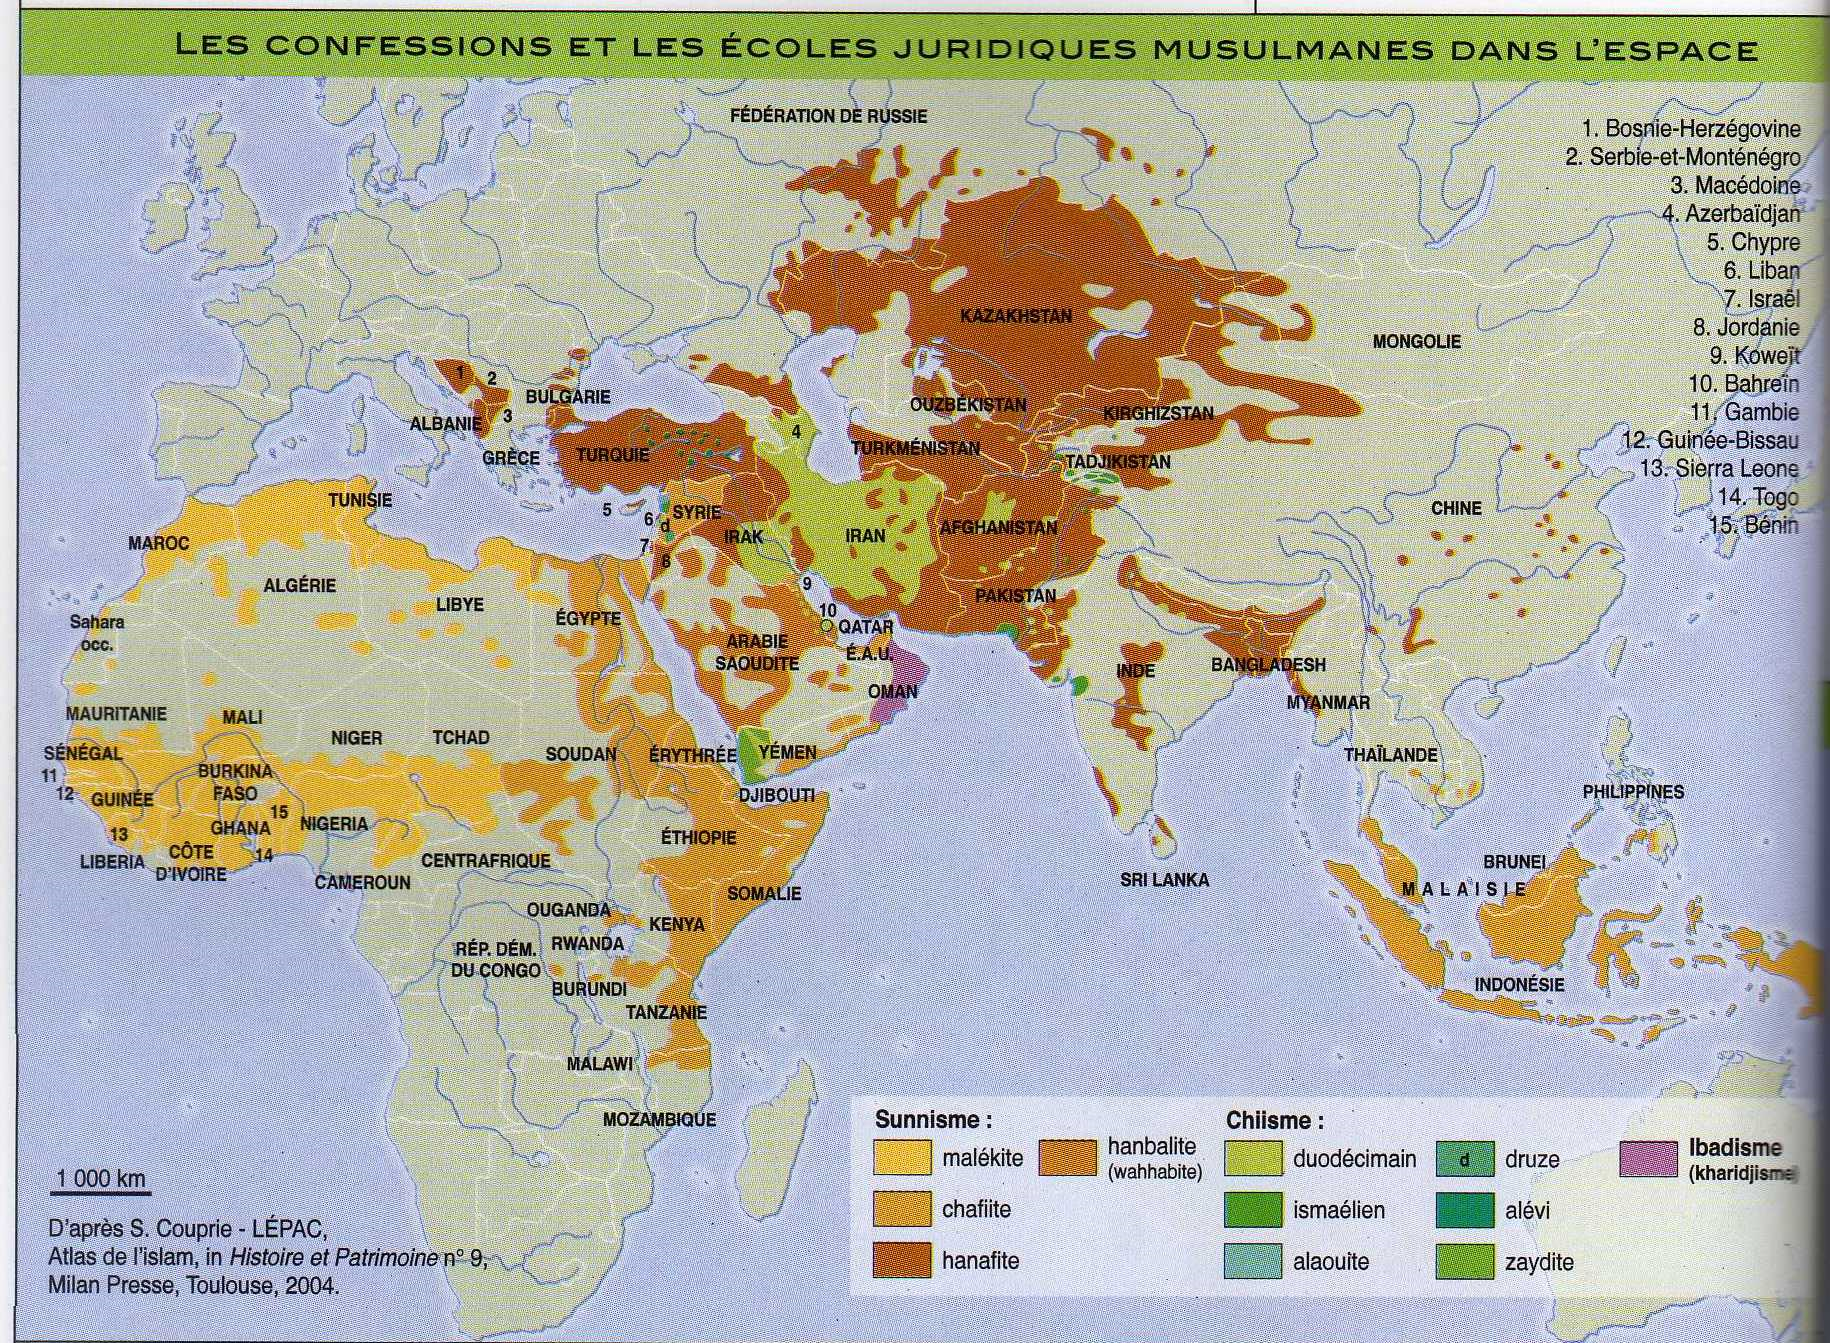
\includegraphics[width=\textwidth]{CourantsIslamContemporain/ImagesCourantsIslamContemporain/CarteSunnisme.png}
 
    \label{fig:my_label}
\end{figure}



\bi 
\item  malékisme : Afrique Nord et ouest.
\item Chafiite : Est de l'Afrique et surtout Egypte 
\item Hanafite : Turquie, asie Centrale, Inde. \textit{les empires turques}
\item Hanbalite : surtout Arabie Saoudite, transformé en \textit{Wahhabisme} au XX, avec une extension au dela de l'Arabie Saoudite en 1960.
\ei 


\subsection{Trois grands courants dans le sh'isme}


\begin{Synthesis}[divergence en Si'isme : les courants]
Des désaccords sur Qui est Imam et sur la \textit{nature de l'Imam}. Il peut être investi de pouvoirs divins.
\end{Synthesis}

\bi 
\item Les duodécimains (ils reconnaissent 12 imams) : les shi'ites Iraniens
\item les Ismaeliens ou septimains (7 imams, l'Aga Khan), Liban.
\item zaydites (5 imams) : Yemen. Au niveau de la doctrine, ils reconnaissent peu de pouvoirs divins aux Imams (proches des Sunnites de ce point de vue).
\ei 
Les Ibadites sont Khajidites. Les druzes et les Alaouites (Alevi en Turc) sont issus du shi'isme (en se proclamant le Maadi) mais ne sont pas considérés comme musulmans par les autres musulmans.  A ne pas confondre à la famille Alaouites au Maroc qui sont tout à fait sunnite (Alaouite veut dire descendant d'Ali). L'Iran reconnait les Alaouites comme shi'ites pour des raisons politiques. 

\subsection{diversité culturelle}
L'islam s'est acculturé aux cultures qu'il a rencontré.
\paragraph{Mosquée}
Le seul élément architectural à une mosquée est la qibla qui indique la Mecque : le Mihrab.

\bi
\item la mosquée bleue a été constituée sur le plan de Sainte Sophie
\item Mosquée de Djenné.
\item La mosquée de Lagos : représente un style baroque brésilien.
\item Xian
\item la grande mosquée de Paris : sur l'image d'une mosquée marocaine
\item Mosquée contemporaine de Créteil

\ei 

\paragraph{L'habit féminin} D'après le Hadith "on ne doit montrer que les mains et le visage". 

\bi
\item les danseuses de cours à Surakarta
\item la burqa, avec grillage sur les yeux, asie centrale et Afghanistan dans certains milieux
\item des vétements de couleur et le shadri, vêtement traditionnel en Asie centrale paysanne voile que l'on met différemment selon qu'on est seul, ...
\item en Afrique, habit d'abord ethnique et non religieux. 
\item En France, les jeunes : le bandeau pour tenir le foulard et le foulard coloré. et certaines ne portent pas le foulard
\ei 

\paragraph{Pourquoi une impression d'uniformisation} La mondialisation crée l'uniformisation et certains courants wahhabites incitent à l'uniformisation sur l'influence saoudite.

\subsection{Observer l'islam}

 
\newlength\q
\setlength\q{\dimexpr .5\textwidth -2\tabcolsep}

\begin{table}[h!]
\sidecaption{\textit{Observer l'Islam} Clifford Geerzt, il a été au Maroc et en Indonésie}
%\begin{tabular}{p[7cm]p[7cm]}
\noindent\begin{tabular}{p{\q}p{\q}}
\toprule
\textbf{Maroc}                                                     & \textbf{Indonésie}                                               \\ 
\midrule
Tribale                                                            & Paysanne                                                         \\
\textit{Audace}                                                    & \textit{Application}                                             \\
une culture préalable moins riche                                  & L'islam est arrivé sur une civilisation hindouiste et bouddhiste \\
Un islam de dévotion aux saints (en particulier le saint guerrier) , austérité morale, pouvoirs magiques, piété agressive & malléable, syncrétique  \\
Uniformisation, facteur de civilisation & diversification, multiforme\\

\bottomrule
\end{tabular}
\end{table}

\subsection{Bibliographie}

\begin{quote}
\textbf{Atlas}

*DUPONT, Anne-Laure \emph{Atlas de l'islam dans le monde}, nouv. éd.,
Autrement, Paris, 2014. GUIDERE, Mathieu \emph{Atlas des pays arabes. De
la révolution aux démocraties}, Autrement, Paris,

2012.
\end{quote}

\hypertarget{ouvrages}{%
\subsection{Ouvrages}\label{ouvrages}}

\begin{quote}
BURESI, Pascal \emph{Géo-histoire de l'islam}, Belin, Paris, 2005.

GEERTZ, Clifford \emph{Observer l'islam : changements religieux au Maroc
et en Indonésie}, La Découverte, Paris, 1992.

*MERVIN, Sabrina \emph{Histoire de l'Islam. Doctrines et Fondements},
nouv. éd., Flammarion, 2016.

DE PLANHOL, Xavier \emph{Les nations du prophète}, \emph{manuel
géographique de politique musulmane}, Fayard, Paris, 1993.
\end{quote}

\chapter{
Le soufisme ou la mystique en islam}


\section{Calligraphie}


\includegraphics[width=\textwidth]{Images/image013.jpg}


« Aux commencements de l'islam, il n'y a ni ascètes ni soufis.
L'ascétisme et la mystique musulmane vont se développer dans les
sociétés de convertis à partir du IX\textsuperscript{e}~siècle. C'est un
phénomène d'hybridation culturelle. Le soufisme est d'abord le fait de
maîtres isolés au IX\textsuperscript{e}~siècle, vivant du côté de
l'actuel Iran. À partir du XII\textsuperscript{e}~siècle se développent
les premières confréries, dont certaines sont encore vivantes
aujourd'hui. Dans l'islam, la mystique est aussi développée que dans le
christianisme, mais elle a été davantage combattue. D'abord par les
juristes, qui voyaient d'un mauvais œil ces croyants qui s'émancipaient
des règles sociales, puis par le wahhabisme, qui les a massacrés dans la
deuxième­ moitié du XVIII\textsuperscript{e}~siècle ».\sn{Jacqueline Chabbi}


« Dans cette calligraphie, j'ai recherché la stabilité mais aussi un
geste plus tendre. Certains y verront peut-être un personnage
agenouillé, en prière\ldots{} Pourquoi pas ? J'offre une image sur
laquelle je ne peux pas toujours mettre des mots. C'est à ceux qui
regardent d'interpréter mes images. Quand je peins, je prends toujours
en considération le blanc laissé par la trace. En calligraphie, un
principe dit :\emph{~``Le noir de votre calligraphie, c'est vous. Le
blanc de votre calligraphie, c'est vous aussi.''}~J'y pense souvent.
Dans les textes anciens, le soufi -- que l'on peut traduire par
``mystique'' -- doit travailler sur soi-même pour retrouver la lumière
intérieure. Il devient alors pur et peut arriver à rencontrer la
divinité. »\sn{Hassan Massoudy}


\section{Introduction}
\paragraph{ Qu'est-ce que le soufisme~?} Pour les soufis, il s'agit de la dimension
spirituelle et originelle de l'islam. Le mot originel est important~: il
signifie que le soufisme est connaturel à l'islam, qu'il est l'islam. Il
ne s'agit pas d'un développement ultérieur qui aurait eu lieu sous
l'influence du monachisme chrétien ou du šī`isme, mais de l'islam vécu
par Muḥammad et ses compagnons. Donc, pour les soufis, Muḥammad est un
soufi. Les salafs, les anciens, les compagnons de Muḥammad sont soufis.
On comprend que si al-Ġazālī \label{theol:AlGazali27} considère le soufisme comme la voie par
excellence pour aller à Dieu, il n'en demeure pas moins que sous sa
plume la référence aux salafs y est importante.
\mn{Le soufisme et Si'isme

\begin{itemize}
\item
  historiquement, plutôt dans l'islam sunnisme
\item
  dans le si'isme, c'est presque intégré tellement il est naturellement
  spirituel.

  \item
    Dans le cadre duodecimain strict, on ne prie pas les imams
  \item
    Mais en fait, il y a des «~sectes~» qui vont le prier, à commencer
    par le fait qu'on va considérer que c'est le «~l'imam caché~»

  \end{itemize}}
Pour autant, cette affirmation d'éminents soufis n'est pas partagée par
l'ensemble des penseurs de l'islam, et au cours de l'histoire, le
soufisme a pu faire l'objet de critiques, de contestations, de
réfutations plus ou moins virulentes. Certaines des pratiques soufies
ont pu être considérées comme hétérodoxes, innovatrices, non conformes à
l'islam des origines. Ce sont ces accusations récurrentes qui permettent
d'expliquer pourquoi on s'en prend aujourd'hui encore à des mosquées
soufies. 
\paragraph{Le wahhabisme est la matrice idéologique anti-soufie
contemporaine}. Comme nous l'avons vu, il est né en Arabie à partir du
18\textsuperscript{ème} siècle en contestant les confréries soufies
jugées non confirmes à l'islam. Aujourd'hui, l'État islamique de l'Irak
et du Levant, au lendemain de la conquête de Mossoul a distribué aux
habitants une charte comprenant 16 commandements~: à l'article 10, il
est écrit que toutes les manifestations publiques contraires à l'islam
sont interdites (article 10). En 2014, quatre sanctuaires sunnites et
soufis et six mosquées chiites ont été détruites dans la province de
Ninive, sous contrôle des insurgés. La destruction la plus spectaculaire
fut celle du tombeau du prophète Jonas -- Yunus en arabe -- qui a été
réduite à un amas de cailloux.

En Égypte, dans le Sinaï, en décembre 2016, un shaykh soufi et un de ses
disciples sont assassinés par le groupe de l'Etat islamique. Le 24
novembre 2017 l'attentat à la mosquée al-Rawdah de Bir al-Abed fait 305
morts -- à cette mosquée était attachée une \emph{zāwiya} -- édifice
religieux fréquenté par des soufis et des conscrits de l'armée. Cette
mosquée soufie appartient à l'ordre soufi des ǧarirites du nom d'Aïd Abū
Ǧarīr qui a fondé trois loges dans le Sinaï au 20\textsuperscript{ème}
siècle dont celle de Bir al-Abed\sn{Sur la sociologie religieuse
  du Sinaï, voir l'article d'Ismaïl Alexandrani~:
   \url{http://orientxxi.info/magazine/-genealogie-du-djihadisme-au-sinai,0687}}.

\vide{i--duxe9finir-le-soufisme}{%
\section{{Définir le soufisme
}}\label{i--duxe9finir-le-soufisme}}

En guise d'apéritif, écoutez la voix d'Henri Corbin (m. 1978),
philosophe et éminent orientaliste français, spécialiste surtout de
l'islam iranien et de la gnose chiite. \emph{Extrait d'un entretien avec
Bernard Maxime Latour en 1971}.

Définition complexe donc, «~tâche scabreuse~»\ldots{} essayons cependant
de le définir à partir de la manière dont les musulmans eux-mêmes
présentent le soufisme, le \emph{tasawwuf} en arabe.

Pour cela, je vous propose de lire un extrait du livre Traité de
Kalābāḏī, \emph{Kitāb al-ta`arruf li-maḏhab ahl al-tasawwuf} qui a été
traduit par Roger Deladrière\sn{~\textsc{Kalābāḏī}, \emph{Kitāb
  al-taʿarruf li-madhhab ahl al-taṣawwuf} {[}traduction française~:
  Traité de soufisme, Les Maîtres et les étapes, traduit de l'arabe et
  présenté par Roger Deladrière, Paris, Actes-Sud, Sinbad, 1981.}.
Kalābāḏī \label{theol:Kalabadi} est un auteur persan, mort aux environs de 990. Cet ouvrage
cherche à réconcilier le soufisme et l'orthodoxie. C'est un classique,
apprécié de tous. En son introduction, il consacre plusieurs pages à
cerner le sens de soufisme par l'étymologie. C'est un peu dense et
technique, mais tout à fait accessible. En ces derniers cours, ce long
extrait vous permet de prendre contact avec un texte fondamental en
islam et avoir la satisfaction d'y être à peu près à l'aise.
\begin{quote}
    

«~Certains ont soutenu que les soufis furent appelés de ce nom à cause
de la pureté (\emph{safā}') de l'intime de leur être et de l'absence de
souillure de leurs actes. Selon Bichr Ibn al-Hârith, «~le soufi est
celui dont le cœur est pur à l'intention de Dieu~». D'après un autre,
«~le soufi est celui dont le comportement est pur à l'égard de Dieu et
dont le charisme (\emph{karâma}) qui lui vient de Dieu -- que soient
proclamées Sa Puissance et Sa Majesté~! -- est pur~».
\end{quote}
Selon une autre explication, les soufis ont été appelés ainsi parce
qu'ils sont, devant Dieu, au premier rang (\emph{saff}), du fait que de
leurs aspirations (\emph{himam}) s'élèvent jusqu'à Lui, que leur cœur se
tourne avec empressement vers Lui, et que l'intime de leur être se tient
en arrêt devant Lui.

D'après certains, ils auraient été désignés du nom de soufis parce que
leurs caractéristiques sont proches de celles des «~hommes du banc~»
(\emph{ahl al-suffa}) qui vivaient à l'époque de l'Envoyé de Dieu -- que
Dieu prie sur lui et le salue !

Selon d'autres, ils furent nommés soufis parce qu'ils portaient un
vêtement de laine (\emph{sûf}).

Ceux qui rattachent leur nom au «~banc~» (\emph{suffa}) et à la
«~laine~» (\emph{sûf}) expriment ainsi l'apparence extérieure de leur
état spirituel. \paragraph{ Ce sont en effet des hommes qui ont délaissé ce bas
monde}, ont quitté leur demeure, ont fui leurs amis, parcourant les pays,
le ventre creux, dénudés, ne prenant des choses d'ici-bas que
l'indispensable pour avoir une tenue décente et calmer leur faim. Parce
qu'ils ont quitté leur demeure on les appelle aussi «~étrangers~»
(\emph{ghurabâ'}), et à cause de leurs nombreux voyages on les désigne
sous le nom de «~pèlerins~» (\emph{sayyâhûn}). Du fait de leurs
pérégrinations dans les régions désertiques et parce qu'ils prennent
refuge en cas de nécessité dans les cavernes, les autochtones les ont
surnommés «~les hommes des cavernes~» (\emph{chikaftiyya}) car le mot
«~\emph{chikaft}~» dans leur langue désigne une grotte ou caverne.

Les Syriens leur ont donné le nom de «~faméliques~» (\emph{jaw'iyya})
parce qu'ils prennent seulement comme nourriture ce qui maintient les
forces dont ils ont besoin, conformément à la parole du Prophète~:
\begin{quote}
"Des aliments qui maintiennent ses forces devraient suffire au fils
d'Adam".~     
\end{quote}
Sarî Saqatî les a décrits en ces termes~: 
\begin{quote}
    «~Ils mangent
comme des malades, ils dorment comme des gens qui font naufrage, et ils
parlent comme des hommes stupides.~»
\end{quote}

Du fait de leur renoncement à la propriété on les a appelés «~pauvres~».
On avait demandé à l'un d'eux ce qu'était le soufi, et il répondit~:
\begin{quote}
   «~Celui qui ne possède pas et n'est pas objet de possession.~» 
\end{quote}
voulant
dire par là qu'il n'était pas l'esclave des désirs. À la même question,
un autre déclara~: 
\begin{quote}
    «~Le soufi est celui qui ne possède rien et qui, si
jamais il vient à posséder quelque chose, le donne.~»
\end{quote}


À cause de leur vêtement et de leur aspect on leur a donné le nom de
soufis, car ils ne portent pas ce qui est doux au toucher et agréable à
regarder, ce qui serait flatter les passions de l'âme, mais uniquement
une tenue décente, se contentant d'un tissu au poil rugueux et d'une
laine grossière.

Tout cela était la condition des «~hommes du banc~», qui vivaient à
l'époque de l'Envoyé de Dieu. Ils étaient en effet «~étrangers~» et
«~pauvres~», des exilés qui avaient quitté leur demeure et leurs biens.
Abû Hurayra et Fadâla Ibn'Ubayd en firent la description suivante~:

\begin{quote}
   «~Ils tombaient de faim à tel point que les Arabes bédouins les
prenaient pour des fous.~» 
\end{quote}
 Ils étaient vêtus de laine, et, au dire de
certains, cela les faisaient transpirer tellement qu'ils exhalaient
l'odeur des moutons qui ont reçu la pluie. Ceci au point que 'Uyayna Ibn
Hisn dit au Prophète~: 
\begin{quote}
   «~L'odeur de ces gens m'incommode, ne
t'incommode-t-elle point toi aussi~?~» 
\end{quote}


La laine est d'ailleurs aussi le vêtement des prophètes (\emph{anbiyā'})
et la mise des saints. C'est ainsi que, selon la parole du Prophète
rapportée par Abû Mûsâ Ach'âri,
\begin{quote}
    «~ soixante-dix prophètes, pieds nus et
vêtus de manteaux de laine, sont passés par le rocher de Rawlâ, et ils
se rendaient au \emph{Temple Antique} (de la Mecque)~».
\end{quote} 

D'après Hasan
Basrî, «~Jésus -- que la paix soit sur lui -- se vêtait de crin, se
nourrissait des fruits des arbres, et passait la nuit là où il
s'arrêtait.~» Selon une autre tradition d'Abû Mûsâ, le Prophète se
vêtait de laine, prenait des ânes comme monture, et se rendait à
l'invitation des pauvres gens. Hasan Basrî disait encore qu'il avait
connu soixante-dix Compagnons ayant combattu à Badr qui ne se vêtaient
que de laine. Ceux qui se comportaient comme les «~hommes du banc~»,
selon ce que nous avons indiqué, ayant les mêmes vêtements et la même
tenue qu'eux, portèrent donc le nom de «~\emph{suffiyya}~» et du
«~\emph{sûfiyya}~» (soufis).

\paragraph{Quand on rattache leur nom à l'élite (\emph{safwa}) et au premier rang
(\emph{saff}), on exprime alors ce qui se rapporte à leur être intime et
à leur état intérieur}. Dieu, en effet, purifie le secret de l'âme et
illumine le cœur de celui qui quitte le monde, y renonce et s'en
détourne. Selon une parole du Prophète,

\begin{quote}
«~quand la lumière pénètre dans
le cœur, il se dilate et s'épanouit.~» On lui demanda «~quel en est donc
le signe, ô Envoyé de Dieu~?~»~; il répondit «~s'éloigner du monde
illusoire, se tourner vers le monde éternel, et se préparer à la mort
avant qu'elle ne survienne.~»    Ainsi le Prophète avait fait savoir que
Dieu illumine le cœur de celui qui s'éloigne de ce bas monde. Et quand
il questionna Hâritha sur la réalité profonde (\emph{haqîqa}) de sa foi
(\emph{imân}), celui-ci déclara~: «~J'ai détaché mon âme de ce monde,
assoiffé pendant le jour, en veillant la nuit, et ce fut comme si je
voyais se dresser le Trône de mon Seigneur, et comme si j'apercevais les
habitants du Paradis qui se rendaient visite et ceux de l'Enfer qui se
repoussaient.~» Selon ce récit, après qu'il se fut détaché du monde,
Dieu lui illumina le cœur, de sorte que ce qui lui était primitivement
caché lui était devenu visible. Le Prophète s'écria alors~: «~Quiconque
veut voir un serviteur dont Dieu a illuminé le cœur n'a qu'à regarder
Hâritha~!~» À cause de ces caractéristiques, de tels hommes ont été
appelés «~illuminés~» (\emph{nûriyya}). Elles étaient également celles
des «~hommes du banc~». Dieu a dit en effet~: «~Il y a là des hommes qui
aiment à se purifier~; et Dieu aime ceux qui se purifient~.~» Il s'agit
de se purifier extérieurement des souillures et de se purifier
intérieurement des pensées qui surgissent dans l'esprit et des idées qui
se meuvent dans la conscience. Dieu a dit~: «~Des hommes que nul négoce
et nul troc ne distraient de l'invocation (\emph{dhikr}) de Dieu.~»
\end{quote}
 

En outre, à cause de la pureté de leur être intime, leur intuition
(\emph{firâsa}) est juste. Selon une tradition du Prophète rapportée par
Abû Umâma Bâhilî~: «~Prenez garde à l'intuition du croyant, car il
regarde avec la lumière de Dieu~!~» Abû Bakr le Véridique avait
déclaré~: «~Mon cœur a reçu l'inspiration que l'enfant porté dans son
sein par Bint Khârija est une fille~»~; et il en fut comme il l'avait
annoncé. De même le Prophète a dit «~La Vérité parle par la bouche de
'Umar.~» Uways Qarâni, salué par Harim Ibn Hayyân, lui rendit ses
salutations en l'appelant par son nom, alors qu'il ne l'avait jamais vu
auparavant~; et il lui dit ensuite~: «~Mon âme a reconnu ton âme.~» «~Si
vous vous entretenez avec les «~hommes de la sincérité (\emph{sidq}),
dit Abû 'Abd'Allâh Antâki, soyez vous-mêmes sincères, car ils sont les
observateurs des cœurs~! Ils pénètrent dans l'intimité de votre âme et
décèlent vos intentions.~»

\paragraph{Quiconque possède de telles qualités~: limpidité de l'être profond,
pureté du cœur, lumière de l'âme, est «~au premier rang~»}, car elles
caractérisent les «~devançants~» (\emph{sâbiqûn}). Selon une tradition
du Prophète~: «~Soixante-dix mille membres de ma Communauté entreront au
Paradis sans Jugement », précisant ensuite «~pour les autres ou pour
eux-mêmes ils n'ont point de recours aux talismans ni aux
cautérisations, mais ils s'en remettent à leur Seigneur avec
confiance.~» À cause de la pureté de leur être intime, de l'ouverture de
leur âme, et de l'illumination de leur cœur, les connaissances qu'ils
tiennent de Dieu sont justes~; ils ne se réfèrent pas aux causes
secondes (\emph{asbâb}), confiants qu'ils sont en Dieu, s'en remettant à
Lui, et acceptant Son Décret (\emph{qadâ}).

Toutes ces qualités et toutes les significations de ces mots se trouvent
réunies dans les noms et les appellatifs désignant la «~communauté
spirituelle~» (\emph{qawm}). Les expressions en sont exactes, et leur
emploi en est facilement compréhensible. Même s'ils diffèrent en
apparence, leur sens est concordant.

\begin{Def}[soufi]
Si on le tire de \emph{safâ'}
(pureté) et \emph{safwa}(élite), le terme qui désigne ces hommes est
alors celui de \emph{safawiyya}. Si on le rapporte à \emph{saff} (rang)
ou \emph{suffa} (banc), ils sont des \emph{saffiyya} ou des
\emph{suffiyya}.
\end{Def}
 Il est possible, dans le premier cas, que la lettre
\emph{wâw} ait été placée avant la lettre \emph{fâ'}, ce qui donne bien
le mot \emph{sûfiyya}(soufis)~; et, dans le deuxième cas, ajouter le
\emph{wâw} à \emph{saffiyya} ou \emph{suffiyya} serait dû à l'usage
linguistique. Si, enfin, on a tiré le mot \emph{sûfiyya} du \emph{sûf}
(laine), il est parfaitement correct, et cette désignation est
linguistiquement juste.

 \paragraph{Ces termes expriment le renoncement et le détachement
de l'âme à l'égard de ce bas monde, le fait de quitter sa demeure et de
voyager sans cesse, de ne pas flatter les passions de l'âme, de purifier
sa conduite, de rendre limpide l'intime de son être, d'ouvrir son cœur,
et de se comporter en «~devançant~». } Ajoutons à cela ce que dit Bundâr
Ibn Husayn~: «~Le soufi est celui que Dieu a choisi pour lui-même et
qu'Il a traité avec affection (\emph{sâfâ}), le libérant de son âme
(égoïste) et lui épargnant dès lors tout effort et toute contrainte en
vue d'un motif personnel. Et le mot \emph{sûfiya~}= il a été traité avec
affection est (un verbe passif) du même type morphologique que
\emph{'ûfiya}~: il a été protégé, à savoir que c'est Dieu qui l'a
protégé, et \emph{kûfiya~}: il a été rétribué, par Dieu, ainsi que
\emph{jûziya~}: il a été récompensé, par Dieu. L'action de Dieu sur lui
est donc manifeste dans son nom même de \emph{sûfî}, et Dieu est seul à
s'occuper de lui.~»

Interrogé sur la définition du soufi, Abû 'Alî Rûdhabâri répondit~:
«~C'est celui qui a revêtu de laine (\emph{sûf}) sa pureté
(\emph{sâfâ}'), qui a fait goûter à ses désirs personnels la saveur de
la privation, et qui, ayant laissé ce bas monde derrière lui, a suivi la
voie de l'Élu (Mohammad).~»

La même question ayant été posée à Sahl Ibn'Abd Allâh Tustarî~: «C'est,
dit-il, celui qui est pur de tout ce qui trouble, qui est rempli de
méditation, qui s'est retiré des hommes pour se consacrer à Dieu, et
pour qui l'or et l'argile se valent.~»

On demanda à Abû-l-Hasan Nûrî ce qu'était le soufisme
(\emph{tasawwuf})~: «~C'est, répondit-il, délaisser tout ce qui flatte
l'âme.~»

Interrogé sur le même sujet, Junayd définit le soufisme~: «~ C'est
purifier son cœur de l'approbation des hommes, abandonner ses tendance
innées, maîtriser les dispositions de la nature humaine, écarter les
incitations égoïstes, fixer en soi les qualités spirituelles, s'attacher
à la connaissance des réalités immatérielles, utiliser ce qui est mieux
pour la vie éternelle, pratiquer le (devoir de) bon conseil envers la
Communauté tout entière, tenir envers Dieu l'engagement de rester fidèle
à la vérité, et suivre l'Envoyé dans (l'accomplissement de la foi).~»

Selon Yûsuf Ibn Husayn~: 
\begin{quote}
    «~Chaque Communauté a une élite, dépôt précieux
de Dieu qu'Il a caché à Ses créatures, et s'il y en a une dans cette
Communauté-ci, ce sont les soufis.~»
\end{quote}

Quelqu'un demanda à Sahl Ibn `Abd Allâh Tustarî~: «~Qui fréquenterai-je
parmi les différents groupes musulmans~?~» «~Tu n'as qu'à fréquenter les
soufis, répondit-il, car rien n'a à leurs yeux une importance exagérée
et ne saurait être totalement désapprouvé. Pour eux, tout acte peut être
interprété, et ils te trouveront des excuses en n'importe quelle
circonstance.~» La même question ayant été posée par Yûsuf Ibn Husayn à
Dhû-l-Nûn~:
\begin{quote}
«~Fréquente, dit-il, celui qui ne possède rien et qui ne désapprouvera
aucune situation dans laquelle tu pourras te trouver, qui ne changera
pas même si toi tu changes beaucoup, car plus tu changeras, plus tu
auras besoin de lui~!~»
\end{quote}
On rapporte également de Dhû-l-Nûn ceci~:
\begin{quote}
    
«~Au bord de la mer, en Syrie,
je vis, dit-il, une femme, et je lui demandai~: «~D'où viens-tu -- que
Dieu te fasse miséricorde~! -- ~?~» Elle me répondit~: «~D'auprès de
gens qui répugnent à reposer leur corps sur une couche, et qui prient
leur Seigneur avec crainte et désir.~» -- Et où vas-tu~? Insistai-je. --
Vers des hommes «~que nul négoce et nul troc ne distraient de
l'invocation de Dieu. -- Décris-les-moi~! Lui demandai-je. Elle se mit
alors à déclamer ces vers~:

\emph{Des hommes dont les préoccupations s'attachent à Dieu, et dont les
aspirations ne s'élèvent vers personne d'autre.}

\emph{Leur quête est celle de leur Maître et de leur Seigneur, et quelle
noble quête que celle de l'Unique, l'Impénétrable~!}

\emph{Ils ne se disputent rien de ce monde, ni rien de ce qui est
excellent, ni nourritures, ni plaisirs, ni progénitures, ni vêtements
somptueux et élégants, ni la joie reposante de rester au pays.}

\emph{Ils ne luttent qu'à la poursuite du lieu éternel dont chaque pas
les rapproche.}

\emph{Ils courent par les étangs et les vallées, et on les rencontre en
nombre sur les hauteurs.}
\end{quote}
\vide{ii--muxe9thode-spirituelle-du-soufisme}{%
\section{Méthode spirituelle du
soufisme}\label{ii--muxe9thode-spirituelle-du-soufisme}}

C'est un itinéraire spirituel qui vise à remonter vers l'être unique, à
quitter la dualité de l'homme, sa duplicité, en vue d'une unification.
Il s'agit d'abandonner la superficialité des choses pour entrer dans la
profondeur de l'intériorité et ne pas être réduit au monde des
apparences.

Dans son \emph{Essai sur le soufisme}, Martin Lings compare le monde à
une pépinière~: tout ce qui s'y trouve a été planté en vue d'être
transplanté ailleurs. La partie centrale de la pépinière est réservée à
des arbres nobles. Ils sont tous en pot et poussent, pas beaucoup, mais
un peu. Mais quand on regarde bien, un des arbres se distingue des
autres. Il est luxurieux, vigoureux, beau. Que s'est-il passé~? La cause
en est invisible. Pour autant, on la devine~: cet arbre a pris racine
dans la terre du jardin à travers le fond de son récipient. Que dit
cette image~? Les arbres sont des âmes et le soufisme est une méthode,
une voie pour prendre racine, pour passer à travers la porte étroite qui
est dans l'âme elle-même et qui débouche sur l'océan de la Divinité. Le
soufi sait qu'il est comme les autres hommes, il sait aussi qu'il est
prisonnier du monde des formes (les pots), mais il sait aussi qu'il est
appelé à la liberté qui l'emporte sur sa captivité.

Le soufisme doit donc permettre de s'enraciner dans l'océan de la
divinité, d'entrer dans la source de la divinité, dans
l'\emph{\underline{origine}} donc. Cette origine est divine,
transcendantale, c'est celle de l'Absolu, de l'Éternel.

\paragraph{Le soufisme est d'abord une méthode~; il est donc un anti-dogmatisme,}
mais il n'est pas sans dogmes. Il ne nie pas le credo musulman, au
contraire~; les soufis ont une profession de foi qu'ils énoncent. Mais
il s'agit de ne pas limiter Dieu à cette profession. Dans cette optique,
le mystique andalou Ibn `Arabī appelle à ne pas se limiter à un credo
particulier. Voici un extrait des \emph{Chatons de la sagesse.} Vous
reconnaîtrez peut-être la voix de Georges Claisse. Dans la suite du
cours, je reviendrai sur cette très grande figure du soufisme.

Voie spirituelle vers Dieu, le soufisme est donc la définition d'une
méthode afin d'atteindre la proximité de Dieu, mais plus encore chez
certains, une union, une unification.

\vide{limitation-du-prophuxe8te}{%
\subsection{L'imitation du
Prophète}\label{limitation-du-prophuxe8te}}

\begin{Def}[Sainteté, suġrā et kubrā]
Le soufisme comme voie initiatique conduisant à la «~proximité divine~»
(\emph{walāya})~distingue selon la sainteté «~mineure~» (\emph{suġrā}),
ouverte à tous les fidèles, et la sainteté «~majeure~» (\emph{kubrā}),
réservée à une élite. 
\end{Def}
Pour parvenir à cette sainteté, la plupart des
soufis invitent à l'imitation du Prophète dans la mesure où il est celui
qui a réalisé cette parfaite proximité. 
\begin{Def}[\emph{nubuwwa}]
prophétie
\end{Def}

Ils posent donc l'existence
d'une relation entre la \emph{walāya} et la \emph{nubuwwa}, la
prophétie, mais si al-Tirmidhī (m. 318/930) accorde à la \emph{walāya}
son autonomie par rapport à la nubuwwa, d'autres au contraire, affirme
qu'il n'est pas possible de s'approcher de Dieu sans la \emph{nubuwwa}. \sn{la question est donc la possibilité de l'usage de la Raison pour accéder à Dieu}

L'hagiographie du Prophète Muḥammad s'est aussi accompagnée d'une
spiritualisation de sa figure~: il est «~l'Homme universel~»
(\emph{al-insān al-kāmil}) qui demeure dans ceux qui l'imitent. Or, la
participation à la «~sainteté prophétique~» permet d'actualiser la
Révélation, autrement dit dans donner les clefs pour chaque époque. Il
s'ensuit un «~Muhammado-centrisme~» car c'est Muḥammad en tant que sceau
des Prophètes qu'il convient d'imiter, de suivre, et donc à qui il faut
obéir. On voit ici que le rapport à la Loi est loin d'être supprimé,
spiritualisé. Au contraire.

 
\subsection{Le souvenir
(\emph{ḏikr})} \label{le-souvenir-dikr}

Le souvenir (\emph{ḏikr}) est au fondement du soufisme.
\begin{Def}[{ḏikr}]
Souvenir,
rappel, invocation, il s'agit de revenir à Dieu, de sortir de l'amnésie
qui guette l'homme, de retrouver le moment où fut scellé le pacte
originel (\emph{mīṯāq}).
\end{Def}
  Cette invocation convient à tout lieu, elle est
la marque d'une adoration continuelle. Le \emph{ḏikr} permet de
retrouver et de vivre de la présence divine.

Le Coran invite à cette évocation, à ce souvenir~: «~Souvenez-vous de
moi et je me souviendrai de vous~» (S. 2, 152). De même, le \emph{ḥadīṯ}
invite à la pratique du \emph{ḏikr}.

Ainsi, par exemple~:

\begin{itemize}
\item
  «~`Les cœurs rouillent comme le fer' dit le Prophète à ses compagnons.
  `Et qu'est-ce qui les fait briller~?' demande l'un d'eux.
  `L'invocation de Dieu et la lecture du Coran'~».
\item
  «~Celui qui invoque son Seigneur et celui qui ne l'invoque pas sont
  comparables l'un à un vivant, l'autre à un mort~».
\end{itemize}

Concrètement, le \emph{ḏikr} consiste à invoquer les noms divins ou à
répéter la première partie de la formule de la \emph{šahāda}~: \emph{lā
ilāha illā Llāh}. Puis, il s'agit de répéter le mot Allāh seul, puis, la
dernière lettre de Allāh, le h\ldots{} dans un seul souffle.

Je vous propose d'écouter {une séance de
\emph{ḏikr}
\url{https://www.youtube.com/watch?v=Xq6bIVtCq14}}\emph{.} 
. Ici, les soufis chantent
ensemble la formule \emph{lā ilāha illā Llāh} sur laquelle se surajoute
une psalmodie. Le rythme s'accélère et indique une forme d'ivresse
spirituelle. Généralement, ces invocations s'accompagnent du balancement
de la tête de gauche à droite et du mouvement des bras.

\url{https://www.youtube.com/watch?v=9BaQunfXPpE}{Ici}, vous avez une
vidéo d'une séance de \emph{ḏikr} dans une confrérie.

\vide{luxe9coute-de-luxe9cho-du-verbe-divin-samux101}{%
\subsection{L'écoute de l'écho du verbe divin
(samā`)}\label{luxe9coute-de-luxe9cho-du-verbe-divin-samux101}}

\begin{Def}[{samā`}]
Le \emph{samā`}, tout comme le \emph{ḏikr} a pour objectif de
réactualiser le Pacte originel. Il s'agit d'écouter la musique comme un
écho de ce pacte scellé. 
\end{Def}
Par la musique, l'écoutant libère son âme pour
trouver Dieu. Il y a une quête d'extase~: c'est le \emph{tawāǧud}. La
fin recherchée n'est pas la musique, mais l'écoute, la musique n'étant
qu'un support pour entendre la parole divine. L'écoute est donc
éminemment spirituelle~mais l'usage de la musique peut être dévoyé et
tombé dans le divertissement. Le soufisme n'est pas en soi favorable à
l'écoute de la musique mais il ne refuse pas usage à des fins
spirituelles. Al-Ġazālī  \label{theol:AlGazali28} considère que le samā` n'est pas en soi licite
ou illicite, et que tout dépend de l'intention (\emph{niyya}) de
l'écoutant. Pour rendre compte de cette ambivalence, le soufi al-Šiblī
(m. 946), connu pour ses excentricités paradoxales, dit du \emph{samā`}
qu'il est 
\begin{quote}
    «~en apparence une source de trouble, mais qu'il recèle un
grand enseignement spirituel (
\TArabe{
السماع ظاهره فتنة، و باطنه عبرة
})
~».
\end{quote}

L'histoire du \emph{samā`} montre qu'il a été associé à la danse, et
qu'il a été aussi assimilé au \emph{ḏikr}.

Ultime remarque~: le \emph{samā`} est une voie, une méthode soufie, mais
il n'est pas reconnu par tous les soufis et bien des maîtres ont aussi
privilégié le silence absolu tels Ibn `Arabi ou les premiers maîtres
šāḏilis.

\vide{la-repentance-tawba}{%
\subsection{{La repentance
(\emph{tawba})}}\label{la-repentance-tawba}}

Le repentir consiste à regretter son péché. Les soufis insistent sur
l'importance des larmes.

Elles sont aussi pleines de signification~: la larme est la goutte qui
s'efface en s'évaporant, après avoir témoigné. Sa disparition est
littéralement une extinction (\emph{fanā'}). Elle est symbole
d'intercession et de transformation\sn{On retrouve chez les
  Aztèques ce symbolisme~: les larmes des enfants que l'on apporte au
  sacrifice étaient dites annonciatrices de la pluie à venir. De même
  les lamentations sont mises en relation avec la miséricorde divine et
  la descente de la manne céleste.}.

Dans le soufisme, les pleurs symbolisent la quête du soufi de vouloir
s'abreuver à la source divine elle-même, de faire descendre la grâce, de
réaliser ainsi la présence divine. Les larmes ne sont pas négatives,
mais elles sont signe d'une espérance, de la promesse d'une joie à
venir. Elles ne sont pas la manifestation d'une séparation d'avec Dieu,
mais surtout un appel à retrouver Dieu, à s'unir à lui.

\vide{la-retraite-spirituelle-ux1e2balwux101}{%
\subsection{{La retraite spirituelle
(\emph{ḫalwā})}}\label{la-retraite-spirituelle-ux1e2balwux101}}

La retraite spirituelle constituait à l'époque antique un «~exercice
spirituel~». Le texte apocryphe intitulé \emph{La théologie d'Aristote}
écrit très vraisemblablement en syriaque au VI\textsuperscript{ème}
siècle et qui est un commentaire (\emph{tafsīr}) de certains passages
des \emph{Ennéades} de Plotin\sn{Pierre Thiellet, «~Notes sur la
  Théologie d'Aristote~» dans Prophyre, \emph{La vie de Plotin}, II,
  Paris, Vrin, 2000, p. 625-638.}, donne pour définition de l'extase le
fait d'être seul avec son âme (\emph{khalawtu bi-nafsi})\sn{Plotin,
  \emph{Ennéades}, IV, 8, 1.}. Il exerça très probablement une influence
dans la théorisation de cette solitude spirituelle. La pratique de la
retraite dans le soufisme renvoie à celle du monachisme chrétien avec
les Pères du désert, où l'éloignement de la ville et de la société était
considéré comme un chemin vers Dieu et un des fondements de l'ascétisme
(\emph{zuhd}). Depuis la \emph{Risāla} d'Abū al-Qāsim al-Qušayrī
(986-1072), toutes les présentations du soufisme intègrent un chapitre
sur les retraites spirituelles, qu'elles soient permanentes ou
périodiques. On appelait ces retraites des «~quarantaines~»
(\emph{arba`īniyya}). Elles étaient comprises comme une \emph{imitatio
prophetae}, à la suite de la retraite de quarante jours de Moïse sur le
mont Sinaï ou de celle de David pour réparer sa faute ou encore bien sûr
de Muḥammad qui allait une fois par an se recueillir (\emph{tahannuṯ})
sur le Mont Ḥirā'\sn{Paul B. Fenton, «~La pratique de la retraite
  spirituelle~», dans Giuseppe Cecere, Mireille Loubet, Samuela Pagani,
  \emph{Les mystiques juives, chrétiennes et musulmanes dans l'Égypte
  médiévale (VII\textsuperscript{e}-XVI\textsuperscript{e} siècles).}
  Interculturalités et contextes historiques, Le Caire, IFAO, 2013, p.
  211-252.}. Vous vous souvenez, c'est pendant un temps de retraite
qu'il reçut la révélation du Coran.

Au livre seizième de l'\emph{Iḥyā'} sur la retraite et la vie retirée
(\emph{`uzla}), al-Ġazālī \label{theol:AlGazali29} indique l'existence d'un débat au sein de la
deuxième génération des musulmans~: certains recommandaient en effet
l'amitié, l'assistance entre les croyants, la fraternité, tandis que
d'autres soulignaient l'importance de l'isolement et de la retraite
spirituelle. «~Fuis les gens comme si tu fuyais le lion~»\sn{\textsc{Al-Ġazālī },
  \emph{Iḥyā' `ulūm al-dīn, op. cit.,} K. 16 (\emph{Kitāb ādāb
  al-`uzla}), B.1, p. 665 {[}V.4, p. 248{]}.} conseille Dawūd al-Ta'i.
On raconte aussi cette histoire à propos de Sahl Ibn al-Ṭustarī (m.
896), grand maître soufi~\sn{\emph{Ibid}., p.666 {[}V.4, p. 251-252{]}}.:
\begin{quote}
    
«~Alors qu'un homme s'avança et lui dit qu'il
voulait lui tenir compagnie, Sahl lui répondit~: `Et si l'un de nous
deux vient à mourir, qui sera le compagnon de l'autre~?' L'homme lui
dit~: `Dieu'. Sahl reprit la parole~: `Qu'il lui tienne donc dès à
présent compagnie'~»
\end{quote}

Mais cette approche spirituelle de la retraite et de la solitude dans la
prière et l'isolement a aussi ses détracteurs. En opposition, on
rapporte les paroles du Prophète Muḥammad~où l'on retrouve le bestiaire
du désert~:

\begin{quote}
«~Satan est un chacal pour l'homme. Comme le chacal il saisit du
troupeau la bête égarée qui s'en est éloignée. Prenez garde aux vallées
et restez attachés aux communautés, aux groupes et aux mosquées~».
\end{quote}

Plus rédhibitoire, ce propos du Prophète de l'islam~\sn{\emph{Ibid}, B.1, ḏ.1, p. 667 {[}V.4, p.
  253-254{]}.}: 
\begin{quote}
   «~celui qui se
sépare du groupe (\emph{ğamā`a}), ne serait-ce que d'un empan, ôte de
son cou l'attache de l'islam » ou encore «~celui qui se sépare du groupe
et meurt mourra en homme de l'époque de l'ignorance
(\emph{ğāhiliyya})~». 
\end{quote}

\paragraph{Quels sont les bienfaits attendus de l'isolement~?}
La retraite permet de se consacrer à l'adoration, à la méditation en se
mettant en confidences intimes (\emph{munāğāt}) avec Dieu, en
privilégiant donc l'intimité avec Dieu plutôt qu'avec une créature.

La retraite permet aussi de se débarrasser des péchés auxquels on
s'expose en fréquentant les gens~: la calomnie, la médisance, la
bigoterie, la duplicité, l'avidité, l'attachement au bas-monde.
Al-Ġazālī \label{theol:AlGazali30} indique que l'habitude des gens consiste à se rincer la bouche
avec l'honneur des gens. La fréquentation conduit à s'accorder avec eux
et à s'exposer à la colère de Dieu. Garder le silence revient à
s'associer à leur médisance car l'auditeur est un médisant. Les récuser,
c'est s'exposer à se faire détester et susciter médisance et calomnie
contre soi, donc la médisance en est redoublée\ldots{}\sn{\textsc{Al-Ġazālī },
  \emph{Iḥyā' `ulūm al-dīn}, \emph{op. cit.,} K. 16, B.2, p. 673 {[}V.4,
  p. 272{]}~}.

La fréquentation des gens nous fait poser des questions vides et
hypocrites. Ainsi quand on voit quelqu'un, on lui demande «~comment ça
va~?~», mais on n'accorde aucune importance à la réponse. L'intérêt que
l'on porte à l'autre dans cette question est faux. Autrement dit, la
fréquentation des gens nous pousse à la duplicité. Al-Ġazālī \label{theol:AlGazali11} voit dans
cette question une innovation blâmable.

Finalement, le critère qui permet de vérifier si la retraite est
\emph{ḥarām} ou \emph{ḥalāl} est celui du bien que l'on retire de
l'autre~de par son beau caractère : «~si tu trouves un convive
(\emph{ğalīs}) qui te rappelle l'image et la conduite de Dieu, alors
attache-toi à lui\ldots{} car c'est là le trésor de l'homme doué de
raison (\emph{ġanīmat al-`āqil})~et le dessein du croyant (\emph{ḍāllat
al-mu'min}) »\sn{\textsc{Al-Ġazālī }, \emph{Iḥyā' `ulūm
  al-dīn}, \emph{op. cit.,} K. 16, B.2, fa.2, p. 677 {[}V.4, p. 285{]}~}.

Troisième bienfait~: celui de l'esprit de querelle et du fanatisme. On
rapporte ce dit de Muḥammad~:
\begin{quote}
    «~Il y aura une époque où pour préserver
sa religion, il faudra fuir de village en village, du sommet d'une
montagne à un autre, d'une pierre à une autre, comme un renard qui
s'échappe. Ce jour-là arrivera quand on ne gagnera sa vie qu'en
commettant des péchés et en désobéissant à Dieu. Alors, à cette époque,
le célibat (\emph{`uzūba}) deviendra licite~»\sn{\textsc{Al-Ġazālī },
  \emph{Iḥyā' `ulūm al-dīn}, \emph{op. cit.,} K.16, B.2, fa.3, p. 677
  {[}V.4, p. 286{]}.}.
\end{quote}

Cependant, al-Ġazālī est le théoricien soufi du juste milieu. Et il
souligne combien vivre en dehors de la communauté peut être l'occasion
de s'enorgueillir. Ainsi, en est-il de cette histoire juive~:

\begin{quote}
«~Un sage {[}parmi les israélites{]} avait rédigé trois cent soixante
opuscules sur la sagesse, si bien qu'il en était venu à penser qu'il
avait été gratifié d'un degré élevé auprès de Dieu. Dieu révéla à son
prophète~: `Va lui dire qu'il a rempli la terre d'hypocrisie et que je
n'agrée en rien son hypocrisie'. Le sage abandonna alors
{[}l'écriture{]} et se retira dans un tunnel sous terre. Il se dit en
lui-même~: `À présent, j'ai atteint le contentement de mon Seigneur.
Mais Dieu révéla à son prophète la parole suivante~: `Dis-lui qu'il
n'obtiendra mon contentement qu'après avoir fréquenté les gens et
supporté leur nuisance'. Le sage quitta son refuge et entra dans les
marchés pour fréquenter les gens, s'asseoir avec eux, partager leurs
repas, déambuler dans les marchés. Dieu révéla alors à son prophète~:
`Maintenant, il a obtenu mon contentement~»\sn{\textsc{Al-Ġazālī },
  \emph{Iḥyā' `ulūm al-dīn}, \emph{op. cit.,} K. 16, B.2, p. 687 {[}V.4,
  p. 312{]}.}.
\end{quote}

Si le soufi doit se retirer dans une cellule en solitude, si c'est là
qu'il se souvient de Dieu, l'enjeu est de parvenir à un état permanent
de retraite intérieure. La démarche se retrouve chez Muḥammad.

Le šayḫ al-`Alawī, soufi algérien qui appartient à la branche
confrérique Šaḏiliya qui a pris naissance au 14\textsuperscript{ème}
siècle et qui met l'accent sur l'invocation du nom de Dieu, a fondé sa
propre confrérie. Sa méthode bien qu'elle s'inscrive pleinement dans
l'esprit de la Šaḏiliya, est aussi originale~:

\begin{quote}
«~La khalwah est une cellule dans laquelle je place le novice après
qu'il a juré de ne pas la quitter pendant quarante jours si besoin est.
Dans cet oratoire, il ne doit rien faire d'autre que répéter
continuellement le nom divin (Allâh) en prolongeant à chaque invocation
la syllabe âh jusqu'à ce qu'il soit à bout de souffle.\\
Préalablement, il doit avoir récité la \emph{shahâdah} (\emph{lâ ilâha
illa Llâh}, « il n'y a de Dieu que Dieu ») soixante-quinze mille fois.

Durant sa retraite, il jeûne rigoureusement tout le jour, ne rompant son
jeûne qu'entre le coucher du soleil et l'aube\ldots{} quelques foqarā'
(mystiques) obtiennent l'illumination soudaine au bout de quelques
minutes, d'autres seulement après plusieurs semaines. Je connais un
\emph{faqîr} qui a attendu huit mois. Chaque matin, il me disait: « Mon
cœur est encore trop dur », et il poursuivait sa ḫalwā. À la fin, ses
efforts furent récompensés. »\sn{Martin Lings, \emph{Un saint
  musulman}, p. 96.}
\end{quote}

\vide{station-maqam-et-uxe9tat-ux1e25ux101l-spirituel}{%
\subsection{{ Station (\emph{maqam}) et état
(\emph{ḥāl}) spirituel
}}\label{station-maqam-et-uxe9tat-ux1e25ux101l-spirituel}}

Il existe dans le soufisme une théorie des états et des stations
spirituelles qui dessinent le cheminement et la progression du soufi.
\begin{Def}[\emph{maqam} (station)]
représente dans l'itinéraire vers Dieu, un
degré de perfection spirituelle obtenu à la suite de l'effort personnel
du mystique.
\end{Def}

 Le \emph{ḥāl} (état) en revanche consiste en une
disposition que l'on ne doit qu'à Dieu: «~Les états, disait Al Qushayrī,
sont des dons, les stations sont des mérites~».
\begin{Def}[\emph{ḥāl}]
Le \emph{ḥāl} est fondamentalement un état passager, éphémère. Le but du
soufi est de transformer le \emph{ḥāl} en état permanent (\emph{maqām}).

\end{Def}
Il faut passer du conjoncturel au structurel. Ainsi, la crainte peut
saisir le croyant à la lecture d'un passage du coran, suite à la
rencontre avec un savant ou un soufi\ldots{} mais cette crainte
ressentie doit habiter le croyant au-delà d'une sensation. Le combat
consiste donc à rendre permanent le \emph{ḥāl}.

\vide{iii--grandes-figures-soufies}{%
\section{{Grandes figures soufies
}}\label{iii--grandes-figures-soufies}}

\vide{ux1e25asan-al-baux1e63rux12b-643-728}{%
\subsection{Ḥasan al-Baṣrī
(643-728)}\label{ux1e25asan-al-baux1e63rux12b-643-728}}

Il est, selon les historiens arabes, le premier soufi. Il semble
cependant avoir été plus ascète que mystique~: il recommandait le mépris
du monde, l'examen de conscience. Pour lui, les spirituels se
reconnaissent à leur désir de Dieu. Il faut savoir se taire~: car parler
rajoute quelque chose à l'absolue transcendance de Dieu et finit par
l'offenser.

Ḥasān al-Basrī n'emploie pas le mot \emph{ḥubb} (amour réciproque). Il
dit~: 
\begin{quote}
    comment je peux dire que Dieu a un amour pour moi~?
\end{quote}
 Il préfère
donc le mot \emph{`išq}~: c'est l'éros, le désir. Mais ce mot ne se
trouve pas dans le Coran. Et le théologien hanbalite al-Ansarī le
refuse. Il y voit une intrusion de la raison humaine. Un bel exemple de
pluralisme en islam sur la question de l'amour de Dieu.

À noter que si le salafisme-wahhabiste combat le soufisme, les
salafistes reconnaissent à Ḥasan al-Baṣrī une autorité en tant
que~transmetteur de nombreux \emph{ḥadīṯs}.

\vide{rux101bia-m.-185801}{%
\subsection{{Rābi`a (m. 185/801)
}{3.2 Rābi`a (m. 185/801) }}\label{rux101bia-m.-185801}}

Elle est la première femme mystique de l'islam, la première soufie, un
premier témoin avec Ḥasan al-Basrī. Elle est née 60 ans après la mort du
Prophète Muḥammad. Il y a deux dates pour sa mort, la première la fait
mourir au milieu du huitième siècle à 55 ans, la seconde à la fin du
huitième siècle à 90 ans. Elle a initié la science de l'amour \emph{`ilm
al-maḥabba.}

Rābi`a n'est pas un prénom, cela veut dire la quatrième~: son milieu
familial était très pauvre et comme elle est la quatrième à être née,
son père l'a appelée La Quatrième. On sait peu de choses sur sa vie de
jeune femme. Fut-elle flûtiste~? prostituée~? Certains biographes le
suggèrent donnant au personnage une plus grande renommée.

Dans l'histoire de la pensée, elle est citée par les grands théologiens.
Ainsi, par exemple, Ğāḥiẓ (m. 867) parle d'elle dans le \emph{Livre des
animaux}. Il rapporte le propos de Rābi`a alors qu'on lui offrait un
esclave pour la servir et elle s'y opposait~: «~J'aurais honte de
demander des biens de ce monde à Celui à qui ils appartiennent ; comment
dès lors les solliciterais-je de gens à qui ils n'appartiennent pas ?~».

Ǧāḥiẓ a souligné la qualité rhétorique du propos (il est spécialiste de
rhétorique) ; il y reconnaît en arabe une éloquence exceptionnelle, une
prouesse rhétorique, mais aussi
une preuve ontologique contre l'esclavage.

Un exemple très connu est celui des deux seaux d'eau~ et des charbons~:
Ici, vous allez entendre la voix de Salah Stétié, un écrivain libanais
qui a traduit dans un français remarquable ses plus beaux poèmes.


\subsection{Pour aller plus loin~: les femmes soufies}

Sulaymī consacre un petit opuscule intitulé \emph{Les femmes soufies},
seconde moitié du 10\textsuperscript{ème} siècle, après le traumatisme
de Ḥallāğ \\


Quelques paroles «~insolentes~»~ (l'expression et de Salah Stétié)

\emph{Sur le paradis}

«~Un jour on récitait devant elle ce verset du Coran~: `Ce jour-là, la
seule occupation des hôtes du paradis sera de se réjouir en compagnie de
leurs épouses, ils se tiendront sous des ombrages, accoudés sur des lits
d'apparat'. Elle dit~: `pauvres gens du paradis, les voilà bien occupés
de leurs femmes~!'~»

\emph{Sur le Prophète}~

«~Aimes-tu le prophète~? Certes je l'aime, mais l'amour du créateur m'a
détourné définitivement de l'amour de toute créature~»

\emph{Sur les deux amours}

\begin{quote}
Je t'aime de deux amours

Amour de mon bonheur et amour digne de toi

Quant à cet amour de mon bonheur

c'est que je m'occupe à ne penser qu'à toi seul

à l'exclusion de tout autre

Et quant à cet autre amour dont tu es digne

C'est mon désir

Que tes voiles tombent et que je te voie

Nulle gloire en moi en l'un en l'autre,

non mais louange à toi pour celui-ci comme pour celui-là\sn{Traduction
  Salah Statié, \emph{Rabi'a de feu et de larmes,} Fata Morgana, 2010.}.
\end{quote}

\emph{Sur le pardon}

«~On lui demande~: `J'ai commis de nombreux péchés, Dieu me
pardonnera-t-il si je me repens~?' Elle répond~: il faut que Dieu te
pardonne d'abord et ensuite tu te repentiras~».

\begin{quote}
Ma coupe, mon vin, mon hôte, sont trois,\\
Et moi que remplit l'amour : je suis la Rabi'a\\
Celui qui verse le vin fait circuler sans cesse\\
la coupe de la volupté et du luxe\\
Si de mes yeux je vois, je ne vois que pour Lui,\\
Si regardée je suis, je suis vue avec Lui.\\
O ! Toi qui me blâmes ! Sa beauté oui, je l'aime~!\\
et par Dieu, mes oreilles n'ont que faire de Ton blâme.\\
Que de nuits délirantes j'ai passées, feu, tourment,\\
et mes yeux se sont fait sources par mes larmes !\\
et aucune de mes larmes n'a pu remonter à sa source\\
mon union avec Lui n'a pas duré.\\
blessé, meurtri, mon œil plus jamais ne s'apaise
\end{quote}

\vide{al-hallux101ux11f-m.-309-922}{%
\subsection{al-Hallāğ (m. 309 /
922)}\label{al-hallux101ux11f-m.-309-922}}

C'est un personnage complexe dont l'évolution religieuse a fait couler
beaucoup d'encre. Louis Massignon lui a consacré sa thèse doctorale.
C'est un mystique musulman, crucifié, criant du haut de sa croix~: «~Je
suis Dieu~»\ldots{} expression de sa doctrine de l'unification
(\emph{ḥulūl}).

Son nom lui vient du métier de son père~qui était cardeur de coton. Ses
disciples l'appelaient \emph{al-Hallâj al-asrâr} c'est-à-dire le cardeur
des pensées secrètes. Il voulait dévoiler les «~secrets de l'union
divine~» (\emph{asrār al-tawḥīd})\sn{Pour sa biographie, je
  m'appuie notamment sur l'introduction de Stéphane Ruspoli : \emph{Le
  Message de Hallâj l'Expatrié}, Collection Patrimoine Islam, Paris,
  Cerf, 2006.}.

Quelles relations entretenait-il avec le calife Mu'tadid (892-902) puis
le calife Muqtadir (m. 932) qui le laissa exécuter~? Quels furent ses
contacts avec le christianisme~? Dans quelle mesure trouva-t-il dans la
figure du Christ et de sa Passion un modèle, alors même que l'islam
réfute la mort sur la Croix de Jésus~? Dans quelle mesure ses voyages au
Cachemire lui ont-ils permis de s'imprégner de la sagesse hindoue~?

Il passera une année entière de retraite à La Mecque, imitant ainsi les
retraites solitaires de Muhammad sur le mont Hira. C'est un prédicateur,
un enseignant. Pour lui, l'islam «~n'est pas seulement la soumission
passive~» devant Dieu, ni l'obéissance aux rites prescrits, mais une
doctrine du salut, de la connaissance, de l'amour~». Il était partisan
de la voie du blâme, et assumait ses provocations. Il disait~ainsi :
«~La mécréance et la foi se distinguent seulement par leur nom, mais en
réalité il n'y a pas de différence entre les deux~». En 902, suite à une
expérience spirituelle très forte, il a la révélation du Nom Suprême de
Dieu. Cette révélation fut à la base d'une profonde mutation. Il résume
sa quête en une formule~: «~Anâ al-Haqq~» - littéralement «~je suis le
Vrai~», je suis Dieu.

 
\paragraph{Ibn Atā}\label{ibn-atux101}

Il est dénoncé comme agitateur politique, accusé de comploter contre la
sûreté de l'État et de tenir des propos hérétiques, blasphématoires. Il
est arrêté en 913. Il comparaît devant le vizir Alî ibn `Îsâ qui le
jugea après interrogation «~complètement ignorant du Coran et des
sciences annexes, droit canonique (\emph{fiqh}), Tradition
(\emph{Sunna}), poésie et philosophie arabe~»\sn{Stéphane Ruspoli,
  \emph{op. cit}. p. 34.}. «~On croit rêver~»~! Ibn Atā convoqué au
tribunal déclara Hallāǧ innocent des charges dont on l'accusait et
déclara sa profession de foi totalement valide. Fou de rage, le ministre
le fit battre et Ibn Atā mourut une semaine plus tard.

Hallāǧ arrive au supplice. Il a 65 ans. Il récite encore quelques vers
du Dîwân. Il fait sa prière sous les yeux de ses compagnons en disant~:
«~Ne vous inquiétez pas de cette affaire, car je reviendrai parmi vous
après trente jours~». Il est crucifié. La forme de la crucifixion dans
sa forme musulmane vient des Perses sassanides qui la pratiquaient
couramment. Elle est plus violente, brutale, spectaculaire que la
crucifixion romaine. Sa prière avant de mourir est marquée par la
compassion et la résignation.

Son biographe Stéphane Ruspoli commente~: «~On aura appliqué à la lettre
contre un des plus grands saints musulmans qui lutta pacifiquement pour
la cause de l'islam et la gloire de Dieu, ce verset sombre du Qoran~:
«~Ceux qui combattent Dieu et son Envoyé, et qui sèment la corruption
sur la terre, leur rétribution sera d'être tués, ou crucifiés~; qu'on
leur tranche les mains et les pieds, ou bien qu'on les bannisse du
territoire. Ce sera leur sanction ici-bas, tandis qu'un grand châtiment
les attend dans l'autre monde~» (5, 33)~» (p.35).

Quelques extraits de ses poèmes

\emph{\textbf{Kâna li qablî ahwâ (p. 101)}}

\begin{quote}
\emph{J'ai abandonné aux gens leur usage et leur religion}

\emph{pour me dédier à ton amour, toi ma religion et mon usage.}
\end{quote}

\emph{\textbf{Al-`ayn tubsiru (p. 102)}}

L'œil aperçoit Celui qu'il aime et puis le perd de vue,

Mais le regard du cœur ne cesse jamais de le contempler.

Quand Il n'est pas avec moi, son souvenir m'accompagne,

et le cœur le voit toujours, bien qu'Il se dérobe à mon œil.

\emph{\textbf{Tala'at as-shams (p. 109).}}

\begin{quote}
Le soleil de Celui que j'aime s'est levé de nuit,

Il a brillé sans plus connaître de couchers.

Le soleil du jour se couche certes la nuit,

Mais le soleil des cœurs ne saurait se coucher.

Celui qui aime le Bien-Aimé vole vers Lui,

si grand est son désir d'aller à sa rencontre.
\end{quote}

\emph{\textbf{Li'l `ilm ahl (p. 128)}}

\begin{quote}
Je suis un orphelin, et pourtant j'ai un Père que j'invoque.

Mon cœur tant que je vis s'afflige de son absence.
\end{quote}

Remarquez qu'il s'adresse ici à Dieu avec le nom de Père.

\emph{\textbf{Anâ man ahwâ (p. 129)}}

\begin{quote}
Je suis devenu Celui que j'aime et Celui que j'aime est devenu moi

Nous sommes deux esprits habitant en un même corps.
\end{quote}

\emph{\textbf{Tafakkartu (p. 153)}}

\begin{quote}
j'ai longuement réfléchi aux diverses religions en tâchant de les
assimiler,

puis je les ai ramenées à un seul Fondement ayant maintes ramifications.

Ne demandez pas à un seul homme de s'en tenir à un culte déterminé,

car cela l'écarterait certainement du Fondement divin assuré.

Ce qu'il réclame, c'est un Fondement lui permettant d'élucider

les nobles idéaux et les hautes conceptions afin de les réaliser.
\end{quote}

\emph{Commentaire~}: Ici, l'universalisme religieux de Hallâj semble
accepter tous les cultes, sachant que tout vient de Dieu qu'il est la
sève, l'essence, le Fondement (\emph{al-asl}) qui se transmet aux
ramification de la foi (\emph{shu'ab al-îmân}).

\vide{ibn-arabux12b-m.-1240}{%
\subsection{Ibn `Arabī (m. 1240)}\label{ibn-arabux12b-m.-1240}}

C'est un maître soufi. Incontournable. Pour lui, la pensée de Hallāǧ
accuse une certaine dualité au moment de l'union qui se trouve résolue
dans l'unification. Sur ce point, Ibn `Arabī lui reproche d'avoir laissé
survivre cette dualité dans l'expérience de l'union. Pour lui, l'homme
n'est plus une négation pure qui montre et démontre la puissance de
l'affirmation de l'un, mais par son existence nécessaire, il est l'image
de son créateur, il le représente.

La création est le néant par essence. Elle est illusoire. Elle ne sera
jamais le réel éternel~: «~Tu prétends qu'un autre qu'Allah puisse jouir
de l'Existence~: c'est le nier, et tu es formellement coupable
d'idolâtrie~». (cf. Léo Schaya, \emph{La doctrine soufique}, p 30).

Dieu est au-delà de la dualité de l'être et du non-être. On ne peut pas
justifier l'existence de la dualité entre Lui et un autre que lui. Il
rejette la distinction entre cause et effet. Tout ce qu'il a créé est
une manifestation de lui.

Le maître a influencé des confréries (\emph{turuq}) notamment la
Ḫalwatiyya. Il représente la tradition savante du soufisme. Pourquoi~?

C'est complexe. Mais il existe des facteurs explicatifs. Ainsi, Ibn
`Arabī aurait prédit la victoire des Ottomans et la conquête de la
Syrie. Il s'ensuit que la dynastie lui a accordé un patronage.

Mais plus sérieusement, l'évolution du soufisme au
13\textsuperscript{ème} siècle, le développement des confréries ont créé
un appel d'air doctrinal. Les fondateurs de ces branches confrériques
que sont al-Jîlânî, al-Shâdhilî, al-Rifâ'ī, al-Badawi\ldots{} tracent
une voie, donnent une orientation spirituelle à leur postérité
initiatique. Mais il n'y a pas d'enseignement substantiel~: Ibn `Arabi
vient compléter ce vide\sn{Chodkiewicz, p. 36.}.

Son enseignement procède fondamentalement du Coran~: «~Tout ce dont nous
parlons dans nos séances procède du Coran et de ses
trésors~»\sn{Chodkiewicz, p. 40.}. Ainsi, il invite son disciple
de sa manière~:
\begin{quote}
«~Plonge dans l'océan du coran si ton souffle est assez puissant/ Et
sinon, borne-toi à l'étude des ouvrages qui en commentent le sens
apparent mais n'y plonge pas~! Tu y périrais car l'océan du Coran est
profond et si celui qui y plonge ne se limitait aux lieux les plus
proches du rivage il n'en reviendrait jamais vers les créatures. Les
prophètes et les héritiers-gardiens (\emph{al-waratha al-hafaza})
prennent ces lieux pour but par miséricorde pour l'univers. Quant à ceux
qui restent en arrêt (\emph{al-wāqīfūn}), qui sont parvenus au but mais
sont restés là sans jamais revenir, nul ne tire profit d'eux et ils ne
tirent profit de personne~: ils ont visé le centre de l'océan -- ou
plutôt c'est lui qui les a visés -- et ils ont plongé pour
l'éternité~»\sn{Chodkiewicz, p. 43.}.
    
\end{quote}

\textbf{On ne soulignera jamais assez l'importance de la lettre comme fondement
de l'interprétation.} Sans la lettre, pas d'interprétation, pas de sens
caché. Et l'accès à cette lettre est réservé à ceux qui ont du souffle.
Ils ne cherchent pas l'au-delà de la lettre ailleurs que dans la
lettre~!

À la question de savoir comment trouver Dieu, il prend l'exemple de
Moïse et de la révélation de Dieu dans le Buisson ardent~: Moïse était à
la recherche d'un feu (S. 20, 10). Tout besoin, toute quête de Dieu, se
manifeste, s'épiphanise sous la figure de son besoin. Mais, dit Ibn
`Arabī~: l'homme qui est dans le désert et a été abusé par un mirage,
qui finit par désespérer de tout, alors celui-là trouve vraiment
Dieu\sn{Chodkiewicz, p. 62.}. «~Dieu ne peut être trouvé que dans
l'absence des choses {[}c'est-à-dire des causes secondes{]} sur
lesquelles nous prenons appui~».

Sur les autres religions~: il dit qu'il faut traiter les livres des
autres religions à égalité.

Chaque croyance est à considérer car elle est aussi singulière que
chaque manifestation de Dieu. Dans son acte de foi, le cœur du croyant
répond au désir de Dieu de se manifester en lui.

Le «~Poème `La religion de l'amour'~»\sn{Ibn `Arabî,
  \emph{Turjumân al-ashwâq}, extrait du poème 11 avec commentaire du
  Cheikh al-Akbar -- qu'Allâh l'agrée~! Traduit par M. Gloton dans
  \emph{L'Interprète des désirs}, Albin Michel p. 147 et 155-158.}~:

\begin{quote}
\emph{Mon cœur est devenu capable}

\emph{D'accueillir toute forme.}

\emph{Il est pâturage pour gazelles}

\emph{Et abbaye pour moines~!}

\emph{~}

\emph{Il est un temple pour idoles}

\emph{Et la Ka'ba pour qui en fait le tour,}

\emph{Il est les tables de la Thora}

\emph{Et aussi les feuillets du Coran~!}

\emph{~}

\emph{La religion que je professe}

\emph{Est celle de l'Amour.}

\emph{Partout où ses montures se tournent}

\emph{L'amour est ma religion et ma foi.}
\end{quote}

\emph{La question de l'infinie miséricorde de Dieu~:}

Elle est au cœur de la théologie d'Ibn `Arabī~: il y a un verset
coranique (S. 7, 156)~: «~Et Ma miséricorde embrasse toute chose
(\emph{wa rahmatī wasi'at kulla shay'in}).

Ibn `Arabī dans les Futuhāt rapporte un dialogue entre Iblis et un
savant (Sahl al-Tustari (m. 896).
\begin{quote}
    «~La dernière chose qu'Iblis déclara à Sahl fut celle-ci~: Dieu a dit
`Ma miséricorde embrasse toute chose', ce qui est une affirmation de
portée générale. Or il ne t'échappe pas que je suis une de ces choses,
sans le moindre doute. Le mot `tout' implique l'universalité {[}de cet
énoncé{]} et le mot `chose' représente ce qu'il y a de plus indéterminé.
Sa Miséricorde m'embrasse donc~»~; À Sahl qui réplique `Je ne pensais
pas que ton ignorance irait jusqu'à ce point', Iblis répond~: `Je ne
pensais pas que tu en serais là~! Ne sais-tu pas, ô Sahl, que la
limitation (\emph{al-taqyīd}) est ton attribut et non le sien~?~». Ibn
`Arabî conclut le récit par cette remarque~: «~Je sus alors qu'Iblis
possédait une science incontestable et que, sur ce problème, c'est lui
qui avait été le maître de Sahl~»\sn{Chodkiewicz, p. 63-64.}.

\end{quote}

\vide{iv--le-soufisme-en-accusation}{%
\section{{Le soufisme en accusation
}}\label{iv--le-soufisme-en-accusation}}

\vide{les-critiques-uxe0-lencontre-du-soufisme}{%
\subsection{Les critiques à l'encontre du
soufisme}\label{les-critiques-uxe0-lencontre-du-soufisme}}


\paragraph{Bibliographie}

Frederick De Jong, Bernd Radtke, \emph{Islamic Mysticism Contested:
Thirteen Centuries of Controversies and Polemics} Leiden, Brill, 1999.

Vous trouverez ci-dessous la recension de l'ouvrage proposée par eric
Geoffroy et publiée dans \emph{Studia islamica}. \\


Un certain nombre de théories ou de concepts posent problème~: qu'en
est-il de l'amour et de la relation entre la créature et le créateur~?
Se pose aussi la question de l'inspiration, des visions des soufis. La
thématique de la lumière muhammadienne (\emph{nūr Muḥammad}) faisait de
lui Le prototype du mystique.

\paragraph{Les hanbalites rejetèrent les interprétations ésotériques du Coran.}

\paragraph{Pour autant, au départ, il n'y avait pas forcément d'incompatibilité.
} Certains mu`tazilites étaient aussi soufis, certains hanbalites étaient
soufis. Ce n'est que par la suite avec une forme d'irréconciliabilité
entre mu`tazilisme et sunnisme que les mu`tazilites critiquèrent les
soufis en tant qu'ils étaient des sunnites.

Ḏū' al-Nūn al-Miṣrī est un célèbre soufi qui fut emprisonné à Bagdad
pour avoir refusé le dogme du Coran créé. Mais il y avait aussi des
rivalités entre écoles mu`tazilites, des nuances. Ainsi, si les
iḫšīdiyya admettaient la possibilité des miracles (\emph{karāmāt}), ils
reconnaissaient que les miracles que l'on faisait porter aux soufis
étaient vus comme un danger possible pour le pouvoir. Souvent,
l'opposition au soufisme était plus sociale et politique que
religieusement fondée.

Les mutazilites dénoncèrent aussi le subjectivisme soufi. Ibn Taymiyya,
le maître hanbalite du 13\textsuperscript{ème} siècle a critiqué le
soufi Ibn `Arabi~et l'a taxé d'«~incarnationnisme~» (~\emph{hûlûl}~) et
de panthéisme. Au 19\textsuperscript{ème} siècle, Mohammed `Abdou, le
réformiste égyptien de la «~Nahdha~», lui-même très attiré par la voie
soufie au début de ses études, a affirmé que le soufisme a
«~\emph{efféminé l'Islam et a nourri la résignation des masses~».} Ibn
Badis, le théoricien algérien de la révolution islamique, s'est opposé à
la prétention de l'Amour pour Dieu et a dénoncé les états spirituels
(\emph{aḥwal}) qui confinaient selon lui au charlatanisme. Et le
philosophe tunisien des Lumières Abdelmajid Charfi, écrit dans son
fameux essai \emph{L'islam entre le message et l'histoire}~: le soufisme
«~est responsable d'avoir entretenu l'esprit de servilité, de fatalisme,
la croyance aux prodiges et miracles attribués aux
«~saints~»~»\sn{Abdelmajid Charfi, \emph{L'islam entre le message
  et l'histoire}, Paris, Albin Michel, 2004, p. 210.}.

De même, le philosophe iranien Soroush a mis en garde contre le
soufisme~:\sn{Alain Roussillon, \emph{La pensée islamique
  contemporaine}. Acteurs et enjeux, Paris, Téraèdre, 2005, p. 155.}.
\begin{quote}
    «~l'inconsistance théorique aussi bien que le danger pratique
de l'autoritarisme structurel qui entacherait la relation de maître à
disciple et qui ne pourrait déboucher que sur un système
anti-démocratique -- les Safavides et Khomeyni lui-même étaient
soufis~»
\end{quote}

Mais Abdelwahhab Meddeb disait aussi du soufisme qu'il est le visage le
plus aimable de l'islam\sn{\textsc{Meddeb}, «~Chemins de la
  connaissance~», France culture~:
  \url{http://www.youtube.com/watch?v=ooFDhYNwJPY}}. Et face au
déferlement de critiques, les maîtres soufis ont aussi pris la plume
afin de répondre à leurs contempteurs. Il en est ainsi du šayḫ algérien
Ahmad al-`Alawī (1874-1934) dans sa \emph{Lettre ouverte à ceux qui
critiquent le soufisme}\sn{Ahmad al-`Alawī, \emph{Qawl al-ma`rūf
  fī l-radd `alā man ankara l-tasawwuf}~: \emph{Lettre ouverte à ceux
  qui critiquent le soufisme,} traduction de l'arabe, notes et préface
  de M. Chabry, Introduction de J. Gonzalez, Paris, Entrelacs, 2011.}.

\vide{la-critique-dibn-arabux12b}{%
\subsection{{la critique d'Ibn `Arabī
}}\label{la-critique-dibn-arabux12b}}
\label{Theo:IbnArabi}
Un jour, alors que j'étais à la librairie \emph{tawḥīd} à Lyon, j'ai
aperçu un livre d'Ibn `Arabī. Le libraire me précisa~: «~c'est le seul.
C'est pas trop dans l'esprit de nos éditions. Lui, c'est un polythéiste
(\emph{sic})~».

Le wahhabisme est très hostile au soufisme et déjà dans les fatwas, `Abd
al-Wahhāb accusait les syriens de l'adorer (\emph{ya`budūna Ibn `Arabī~:
ils adorent Ibn `Arabī})\sn{Muḥammad `Abd al-Wahhāb,
  \emph{Maǧmū`at al-fatāwā wa-l-rasā'il wa-l-aǧwiba}, Beyrouth, 1987, p.
  46, cité par Michel Chodkiewicz, «~Le procès posthume d'Ibn `Arabī~»
  dans Frederick De Jong, Bernd Radtke, \emph{Islamic Mysticism
  Contested: Thirteen Centuries of Controversies and Polemics} Leiden,
  Brill, 1999, p. 93.}. La critique d'Ibn `Arabī est parfois assumée et
admise aujourd'hui au sein même des confréries soufies qui, soucieuses
d'orthodoxie, voient en Ibn `Arabī un «~étranger de l'islam~». Mais de
quoi s'agit-il~? Que lui reproche-t-on~? Si la controverse ne date pas
de son vivant, on doit d'abord à Ibn Taymiyya d'avoir écrit le
réquisitoire le plus virulent contre Ibn `Arabī. Un de ses ouvrages les
plus exhaustifs est \emph{Ḥaqīqat maḏhab al-ittiḥādiyyīn}, \emph{La
vérité de l'école des partisans de l'unification}.

Comme souvent, le propos y est nuancé, contrairement à ce que l'on a
véhiculé de lui et il déclare que si la doctrine d'Ibn `Arabī est du
\emph{kufr}, il est le plus proche de l'islam et ses propos sont souvent
excellents.

On trouve quatre condamnations :


  \paragraph{La doctrine de la \emph{waḥdat al-wuǧūd}}, l'unité de
  l'existence. C'est l'idée que l'être de Dieu est l'être de tous les
  êtres et que donc, l'être de Dieu est l'être des djins, des démons,
  des infidèles, des chiens et des porcs. À noter que ceux qui
  soutiennent cette doctrine refusent la doctrine de l'unification
  (\emph{ittiḥād}) qui suppose l'existence d'une dualité qu'ils
  rejettent. À remarquer que l'expression \emph{waḥdat al-wuǧūd} ne se
  trouve pas chez ibn `Arabī~!

La doctrine découle de l'interprétation du \emph{ḥadīṯ qudsī} (nous
avons déjà défini ce qu'est un \emph{ḥadīṯ qudsī})~:
\begin{quote}


« Mon serviteur ne s'approche de Moi par rien de plus excellent que ce
que Je lui ai mis à charge comme œuvres obligatoires. Et mon serviteur
ne cesse de s'approcher de Moi par des œuvres surérogatoires jusqu'à ce
que Je l'aime, et lorsque Je l'aime, Je suis son ouïe par laquelle il
entend, sa vue par laquelle il perçoit, sa main par laquelle il saisit,
et son pied avec lequel il marche. S'il me demande, Je lui accorderai
certainement ce qu'il demande, et s'il cherche refuge en Moi, Je lui
accorderai certainement Ma protection ».
\end{quote}

Pour Ibn `Arabī, il y a donc identification totale entre Dieu et son
serviteur. Mais c'est plus une identité qui n'est pas en devenir. Elle a
toujours existé, mais le serviteur (\emph{`abd}) n'en avait pas
conscience.

\paragraph{la doctrine de la \emph{waḥdat al-adyān~}:} elle consiste à ne
plus différencier l'\emph{imān} du \emph{širk} (la foi de
l'associationnisme, mais là ce devrait être assimilé, c'est juste pour
ceux dont la mémoire n'a plus 20 ans). Le diable lui-même est un lieu
théophanique, et il faudrait donc l'honorer.

\paragraph{la doctrine de la non-éternité des châtiments} des damnés~:
ils ne quitteront pas l'enfer, mais la miséricorde les enveloppera
aussi, elle qui «~embrasse toutes choses~» S.7, 156. C'est la version
musulmane de la doctrine de l'apocatastase (idée que tout sera
réconcilié, Dieu sauvera tout le monde). Elle est rejetée car elle
entraîne une diminution de la crainte de Dieu et ouvre la porte à toutes
les turpitudes.

\paragraph{l'hagiologie d'Ibn `Arabī}~: c'est la question de la
\emph{ḥaqīqa muḥammadiyya} et de son identification au \emph{qalam}, ou
la notion de sceau de la sainteté (\emph{ḫatm al-walāya}) qui
attenterait à la dignité du Prophète.



%\includegraphics{Images/image097.png}
\vide{ruxe9ponse-soufie}{%
\subsection{Réponse soufie}\label{ruxe9ponse-soufie}}

Je vous propose de lire la lettre du Cheikh Ahmad al-Alawī
(1874-1934)~intitulée «~Lettre ouverte à celui qui critique le
soufisme~».

\vide{v--les-ordres-confruxe9riques}{%
\section{Les ordres
confrériques}\label{v--les-ordres-confruxe9riques}}

Il y en a une cinquantaine dans le monde.

\begin{itemize}
\item
  \textit{La qādirīya} \label{Def:Soufiqādirīya}
Fondateur~: `Abd al-Qādir al-Ğīlānī (m. 1166)
Implantation~: dans tous les pays musulmans, du Maghreb à la Chine


\item
  \textit{La Naqchabandīya} \label{Def:SoufiNaqchabandiya}
Fondée au milieu du XIV° siècle
Implantation~: du Caucasse au Turkestan et à l'Inde
Elle a nourri le nationalisme kurde


\item
  \textit{La Šāḏilīya} \label{Def:Soufisadiliya}
Eric Geoffroy dit de la \emph{Šāḏiliyya} qu'elle est l'une des
«~voies-mères~» du soufisme. Elle est apparue entre la fin du
XII\textsuperscript{e} siècle et le XIV\textsuperscript{e} siècle.
D'origine maghrébine, elle s'est diffusée au XIII\textsuperscript{e}
siècle, à partir de l'Égypte, dans la majeure partie du monde musulman.
Son enseignement est dense et il s'appuie sur les écrits d'Ibn
\emph{`}Arabī.
\end{itemize}
Toute voie initiatique a pour but de mener ses adeptes vers la sainteté,
ou «~proximité divine~» (\emph{walâya})~; celle-ci est identifiée au
plus haut degré de la gnose par al-Shâdhilî. De façon schématique, les
premiers maîtres shâdhilis distinguent deux niveaux~: la sainteté
«~mineure~» (\emph{sughrâ}), ouverte au public large des fidèles, et la
sainteté «~majeure~» (\emph{kubrâ}), réservée à une élite spirituelle.
Mais le terme \emph{walâya}, tout comme celui de sainteté en français,
est un terme générique, un idéal qui implique une méthode pour y
parvenir.

Pour les Shâdhilis, la réponse est claire~: c'est dans l'imitation
intérieure du Prophète que se réalise la \emph{walâya}. Réapparaît ici
le débat millénaire sur les rapports entre \emph{walâya}et
\emph{nubuwwa}, la prophétie, débats qui ont partagé exotéristes et
ésotéristes de l'islam, mais aussi les milieux soufis. Autant les
maîtres shâdhilis initiaux se réclament du premier théoricien de la
sainteté en islam, al-Hakîm al-Tirmidhî (m. 318/930), autant ils s'en
éloignent lorsque celui-ci accorde à la \emph{walâya}une autonomie par
rapport à la \emph{nubuwwa}~: pour eux, la première est subordonnée à la
seconde, et puise sa substance même dans la Lumière muhammadienne
(\emph{al-nûr al-muhammadî}).

\begin{itemize}
\item
  \textit{La Bekt'āchīya}
Elle impose le célibat
De nombreux affiliés en Turquie et Albanie


\item
  \textit{La Tidjānīya}
Influente au Maghreb et dans l'Afrique occidentale


\item
  \textit{La Chattārīya}
Influente en Inde et Malaisie

\item
  \textit{La Rah'mānīya}
La plus influente confrérie algérienne.


\item
  \textit{La mawlāwīya} (derviches)
\end{itemize}

Il existe plusieurs ordres soufis, mais l'on peut distinguer deux grands
groupes de mystiques~: ceux qui se trouvent dans la station de l'ivresse
(\emph{sukr}) et ceux qui sont dans la station de la sobriété
(\emph{sahw}).

Les initiés ivres sont souvent les disciples d'Abū Yazīd Bistamī (m.
875)~: l'ivresse, c'est la perte de sens commun, de la maîtrise de soi.
L'âme est enivrée de la connaissance de Dieu, plongée dans la
contemplation de Dieu.

Pour le second groupe, l'ivresse n'est qu'un état transitoire. Elle est
le début de l'unicité, mais elle se caractérise par la sobriété, quand
il sait que le soi n'est qu'un miroir dans lequel se réfléchit l'Essence
divine.

\paragraph{Pour aller plus loin}

Martin \textsc{Lings}, \emph{Qu'est-ce que le soufisme~?} traduit de
l'anglais par Roger du Pasquier, Paris, Éditions du Seuil, 1977.

Eric \textsc{Geoffroy},
«~\url{http://www.facebook.com/topic.php?uid=21148739744\&topic=3226}{L'islamité
du soufisme et son apport à la spiritualité universelle}~» dans
\url{http://www.religioperennis.org/documents/geoffroy/islamitesoufisme.pdf}

Eric \textsc{Geoffroy}, \emph{Initiation au soufisme}, Coll. L'espace
intérieur, Paris, Fayard, 2003.

Alberto Fabio \textsc{Ambrosio}, \emph{Vie d'un derviche tourneur}.
Doctrine et rituels du soufisme au XVII\textsuperscript{e} siècle,
Paris, CNRS Edition, 2010, 1 vol., 406 pages.

Laleh \textsc{Bakhtiar}, \emph{Le soufisme}. Expressions de la quête
mystique, Paris, Seuil, 1977.

Christian \textsc{Bonaud}, \emph{Le soufisme al-taṣawwuf et la
spiritualité islamique}, Préface de

Michel Chodkiewicz, Maison Larose, IMA, 1991.

\textbf{Exercice pour la Validation}

À partir de la lettre du šaḫy Ahmad al-Alawī, identifierez les éléments
qui répondent aux critiques adressées aux soufis et à Ibn `Arabī tels
que nous les avons exposés.



\chapter{Les racines de la réforme : le
renouveau islamique des XVIIe-XVIIIe
siècles}
\mn{(24/01/2022)}

Un leçon sur les racines de cette diversité, et de tous ces courants au sein du monde Sunnisme. Tout cela part du désir de "\textit{Réforme}" qui part à un retour au source. Et cela peut donner des solutions très diverses, soit des lectures libérales ou des lectures fondamentalistes (un peu comme les évangéliques protestants).
Plutôt \textit{Renouveau} que \textit{Réforme}.

%------------------------------------------------
\section{La crise interne du monde musulman}
\subsection{Déclin des grands empires}

 
 \begin{Synthesis}[Date Symbolique]
 1798 : Napoléon en Egypte, date symbolique de la rencontre du monde musulman avec la modernité occidentale.
 \end{Synthesis}
 Cette lecture n'est pas fausse et va donner lieu au \textit{réformisme} mais c'est une lecture occidentalo-centrée.
 En réalité, cela a commencé plus tôt. Un désir né courant XVII et interne au monde musulman.
 
Les trois grands empires musulmans de l'époque rentrent en crise : 

\begin{table}[h!]
    \sidecaption{Les trois grands Empires musulmans}


%\newlength\q
\setlength\q{\dimexpr .25\textwidth -2\tabcolsep}
\footnotesize%
\noindent\begin{tabular}{p{\q}p{\q}p{\q}p{\q}}
\toprule
                & Fondation           & Apogée                            & Fin                                                                                \\
\midrule
Empire Safavide & 1501 (Ismaïl   1er) & Abbas Ier (1588-1629)             & 1736                                                                               \\
Empire Moghol   & 1526 (Babur)        & Akbar (1556-1605)                 &  1857 (existence symbolique après 1761)  \\
Empire Ottoman  & 1299 (Osman 1er)    & Soliman le Magnifique (1520-1566) & 1922                                        \\
\bottomrule
\end{tabular}


    \label{tab:my_label}
\end{table}
 
 
 
 \paragraph{Raisons économiques} Les portugais contournent l'Afrique et contournent les empires musulmans.  
 \paragraph{crises politiques} au sein de ces empires, trop grands. 
 \paragraph{Des voisins puissants} Ces Etats vont perdre des territoires face à des puissances qui ne sont pas musulmanes. L'empire Safavide est attaqué par les Ousbeks. L'Empire Moghol en XVIII siècle s'effondre devant l'empire Marathe (Hindou). L'empire Ottoman resiste mais décline depuis 1686 (siège de Vienne). 
 \begin{itemize}
     \item  {Affaiblissement des sultanats Indonésiens} face aux Hollandais. Java est annexé en 1800. 
  \item {En Chine} les musulmans Chinois (Hui) subissent des pressions des Manchous.
   \item  {Afrique} Les bambaras conquièrent Djenné, Tombouctou et Gao. Les portugais en Océanie. 
  \item {En Asie Centrale}, avancée des Russes (XIVII : Kazakstan et reste de l'Asie Centrale au XIX).
 \end{itemize}

 \paragraph{A la fin du XVI} 1591 : deuxième millénaire de l'Islam; sentiment millénariste. \mn{Calendrier lunaire, donc décalage}
 
 
 
\subsection{Problèmes doctrinaux et religieux}

\paragraph{Un raidissement des écoles juridiques au XVII}
Elles s'accusent les unes les autres de ne pas être juste, sentiment de division du monde sunnite.

\paragraph{Décadence du monde Soufi} On a tendance à considérer les soufis comme à la marge du monde musulman. Pourtant, elles ont joué un rôle social déterminant voire politique. Or, à l'époque, elles sont en crise.
\begin{itemize}
    \item {En faisant des Etats dans l'Etat} 
\item {Laxisme spirituel} Un soufi n'est plus tenu de suivre les prescriptions de l'Islam.
\item {Un rôle de plus en plus important du Sheykh}, le maitre spirituel de la Confrérie, qui transmet la \emph{Baraka}.
\item {Des pratiques spéctaculaire} Le fakirisme. le \emph{Dhikr}, rappel du nom de Dieu et l'on atteint l'Etat de transe, et vont marcher sur des braises. 

\end{itemize}



%------------------------------------------------
\section{L'aspiration au
  renouveau}
\subsection{Millénarisme}


 \begin{Def}[rapport au temps Involutif]
 L'Islam se tourne vers le passé, en Islam, les prophètes viennent toujours rappelés ce qui a été donné à l'origine. et le problème est que les hommes déforment le message transmis. Donc Dieu envoie de nouveaux prophètes pour restaurer le message originel. \textit{le temps corrompt.}
 
 \end{Def}
 vs Evolutif. 
 
 Ce qui fait que Mohammad est le dernier des prophètes, c'est que le message est transmis intact, pour la première fois, donc plus besoin de nouveaux prophètes. Autant, la \textit{pratique} peut se corrompre. 
 Un hadith dit : 
 \begin{quote}
     Slt un dixième de la pratique suffira pour sauver le monde.
 \end{quote}
 
 \begin{Def}[Moujaddid]
 de la racine JDD, nouveau, celui qui renouvelle l'Islam pour le mettre tel qu'il était à l'origine. 
 \end{Def}

 
 \begin{Def}[tajdid]
 Tajdid, le renouveau, qui doit venir régulièrement. Chaque siècle Dieu envoie un \textit{Moujaddid} selon un Hadith du Prophète.
 \end{Def}
 
 
 Il peut y en avoir plus mais à chaque siècle, il y a un grand moujaddid, savant, qui ne fait pas forcément au sein de la communauté. 
  \begin{Ex}
 Ghazali est considéré comme un Moujaddid
 \end{Ex}
 
 
 \subsection{Quelques grandes figures de la \textit{pre-Reforme}}
 

\paragraph{Ahamad Sirhindi} (Inde, 1564-1624) , essaye de rénover l'Islam et réforme une confrérie, la \emph{Naqshbandiyya} réformée (mujaddidi). 
\paragraph{Muhaddidi} Restaurer le monde musulman et restaurer l'Islam dans sa pureté originelle. Il va opposer 
\begin{itemize}
    \item le \emph{taqlid}, l'imitation (péjorative, servile, non réfléchie) et
    \item l'\emph{ijtihad}, l'effort d'interprétation du Coran et de la Sunna. Retourner aux sources scripturaires pour restrouver le sens authentique de l'Islam
    \item pour éliminer la \emph{bid'a}, très péjoratif, l'innovation
\end{itemize}  

On peut distinguer deux courants : un courant plus libéral et l'un plus fondamentaliste :
\begin{itemize}
    \item le rapport à la Tradition : fondamentaliste ne vont considérer que le Coran et la Sunna, en critiquant les élaborations savantes de l'Islam. 
    \item ce sur quoi va porter l'\emph{ijtihad}, soit limité sur les versets peu clairs du Coran, soit plus large pour le savant et les différentes sciences qui vont être convoquées pour l'ijtihad.
\end{itemize}


\paragraph{Muhammad 'Abd Al-Wahhab } 'Arabie, 1703-1792). Voir p. \pageref{Theol:AlWahhab}

\paragraph{Shah Wali Allah} (Inde, 1703-1762), \label{Theo:waliAllah} a eu les mêmes professeurs que Al-Wahhab ! et l'un des premiers à traduire le Coran dans une langue vernaculaire (en persan). Effort d'acculturation dans le contexte Moghol et Indou. 




 
%------------------------------------------------
\section{Les voies du renouveau} 
\subsection{Les confréries soufies}

La création de néo-confrérie
\begin{itemize}
    \item lutter contre un laxisme moral
    \item lutter contre le pouvoir du Sheykh.
    \item insister sur le côté social, en prenant en charge la société (vs gnosticime ?).
\end{itemize}
\mn{Soufi : \pageref{Def:SoufiNaqchabandiya}, \pageref{Def:Soufiqādirīya} }




\paragraph{Ahmad Al Tijani} (Algérie 1737, 1815). Et fonde la \emph{\textbf{tijaniyya}}, un groupe toujours très présent en Afrique du Nord. Normalement un Sheykh insiste sur la chaine d'initiation qui remonte au prophète. Lui, va être initié directement en rêve par le Prophète.

\paragraph{Abdurrauf al-Singkili} (Aceh, Indonésie, 1615-1693)

\paragraph{Abdelkarim al-Samman} (Soudan, 1718-1776) => sammaniyya

Au sénégal, aussi une confrérie de type réformée. 
\mn{A completer carte Carte moderne. Il y avait 24 confréries soufis en Arabie avant le Wahhabisme}




%---------------------------------------
\subsection{Les centres de pèlerinage : La Mecque et Médine}

La Mecque et Médine jouent un rôle essentiel, du fait du Hajj. Du fait de l'Empire Ottoman, il y a pacification des parcours du pélerinage, par ailleurs incités par l'Empire.
Et par ailleurs, des centres de formation s'implémentent à la Mecque.  On en profite pour étudier. Se croisent des savants de différentes origines.
Non seulement les centres d'étude mais aussi les confréries, avec leur Sheykh les plus importants s'installant à Médine ou la Mecque. Ils sont initiés à l'enseignement Moujaddidi et vont réformer la confrérie à laquelle ils appartiennent, selon un modèle qui se répète.




%------------------------------------------------
\section{Un aspect particulier : les jihads aux marges du monde   musulman} 


\begin{figure}[h!]
    \centering
        \sidecaption{Le « renouveau » des marges du monde musulman (XVIIIe-XIXe
siècle)  \emph{L'atlas de l'islam depuis 1500}, F. Robinson, Nathan, 1987  
Des petits Etats vont se créer sur des bases confrériques et dont la mission de faire le jihad.
}
 \includegraphics[width=\textwidth]{CourantsIslamContemporain/ImagesCourantsIslamContemporain/image1.jpeg}

    \label{fig:le-renouveau-des-marges-du-monde-musulman-xviiie-xixe-siuxe8cle}
\end{figure}


\subsection{Situation particulière des zones marginales}


Pourquoi on les retrouve aux marges du monde musulman ? Il y a un besoin de purification et l'islamisation par rapport à des populations hétérogènes. Mais aussi, parce que ces zones ne sont pas controlées par les grands empires musulmans qui ne tolèrent pas ces confréries.
Le jihad se porte d'abord sur les musulmans eux-mêmes, pour qu'ils deviennent musulmans puis contre les puissances extérieures ou non musulmanes qui controlent ces zones. 

\paragraph{Une structure Etatique} Le Sheykh est le chef, \emph{Commandeur des Croyants} - on fait référence aux premiers temps musulmans, on prête allégeance, et avec une approche puritaine, très forte pratique. \mn{Des analogiques avec DAESH, qui se réfèrent eux aussi aux temps de l'Islam}

\paragraph{Une accélération de l'Islamisation}


\subsection{Quelques exemples}

\paragraph{Spectre Temporel 1680-1920}{1680, Etat de Bondou} Afrique de l'Ouest jusqu'e l'Etat Mahdiste (Somalie) 1899-1920.

\paragraph{Chine - Ma Ming-hsin} Réveil religieux des communautés chinoises sous la pression des Manchous. Ma Ming-hsin (1719-1781) lorsqu'il est à la Mecque, il fonde une confrérie réformée, la \textit{Nouvelle Secte} et entre en opposition contre les autorités locales, qui appelle en soutien la dynastie Manchoue des Ming. Ming-Hsin est décapité. Il y aura d'autres révoltes plus tard, du Kan-Su et du Chen-Si (1862) et du Yunnan (1856)

\paragraph{Indonésie - Jajji Miskin} Le mouvement Padri à Sumatra (1803-1845). Après le Hajj, en 1803, il prend le contrôle de villages et va imposer sa vision de l'Islam, interdit les pratiques populaires et proclament le Jihad contre les autres villages et les pouvoirs. 1820 : les Hollandais reviennent dans la région et on a une transformation de ce mouvement contre un Jihad contre les Hollandais. Eliminé par les Hollandais.

\paragraph{Nigéria - Califat de Sokoto} Uthman da Fodio (1755-1817) issu d'une famille de savants musulmans, l'enseignement lui vient par la fraderyya\sn{revoir} et crée une communauté qui le reconnait comme \textit{commandeur des Croyants}, s'oppose aux pouvoirs locaux et va être défait par la Grande Bretagne.


\begin{Synthesis}
\begin{itemize}
Ce renouveau : 
    \item Avant la rencontre de l'Occident
    \item lié à des thèmes de crises internes
    \item des thématiques que l'on retrouvera : retourne aux sources scripturaires
    \item C'est assez fascinant de voir la circulation des idées, liée autour du \textit{Hajj}
\end{itemize}


\end{Synthesis}

%------------------------------------------------

 



 



\paragraph{Soufis du Badakhshân : un renouveau confrérique entre
l'Inde et l'Asie centrale}
\mn{Alexandre Papas, \emph{Cahiers d'Asie Centrale}, n° 11-12, 2004, p.
87-102 (extraits -- texte expurgé)}
 
 
\subparagraph{Éléments de biographie d'un soufi
badakhshânais} 
\mn{le Badakhshân est entre l'Afghanistan et le Tajikistan}
\begin{quote}
Mawlânâ Mîr Ghiyâs al-Dîn \label{Theo:MawlanaMirGhiyasAlDin} naît en 1117/1705-06 dans la petite localité
de Hisârak, située au cœur du district de la ville de Jirm. Le
grand-père de Mawlânâ a émigré du village de Dahbîd, non loin de
Samarcande, en direction du Badakhshân. La \emph{silsila}\sn{Génération} de la famille
remonte au Prophète et, sur dix générations, au frère d'un grand saint
Kubrawî et découvre une généalogie \textit{soufie}. C'est donc au sein d'une des
grandes familles \emph{muhâjir}\sn{Emigré, en référence aux premiers musulmans qui ont suivi le Prophète à Médine} de l'aristocratie religieuse du
Badakhshân que naît Ghiyâsî.

{[}\ldots{]}

C'est précisément pour l'Inde -- destination qui concurrence la
Transoxiane savante, en particulier Boukhara, surtout depuis le XVIe
siècle -- que part le jeune Ghiyâsî âgé de 14 ans en quête d'initiation \sn{soufi}.
Cet exil de l'adolescent fait l'objet de deux contes hagiographiques :
 

\begin{itemize}
\item
 
  Le futur shaykh de Ghiyâsî, Shâh Walî Allâh, qui a quitté Sirhind pour
  entreprendre un pèlerinage au mausolée de Bahâ' al-Dîn Naqshband\sn{le fondateur de la confrérie réformée Naqshandayyi} non
  loin de Boukhara, stationne au Badakhshân, à Jirm, chez le père même
  de Ghiyâsî. Le shaykh demande alors à ce dernier de lui amener ses
  enfants, mais perçoit par claire-vue qu'on lui dissimule le jeune
  Mawlânâ qui, en état de \emph{majzûb}\sn{Ils peuvent faire des choses indécentes} « ravi en Dieu », suscite la honte de
  sa famille. À sa vue le shaykh indien cite un vers de Ni'mat Allâh
  Walî Kirmânî. Et au jeune Ghiyâsî de prononcer miraculeusement le
  second vers du distique. Walî Allâh annonce alors qu'à son retour de
  Boukhara il prendra le jeune homme comme disciple et l'emmènera en
  Inde.
  
\item
 
  Dès l'âge de 9 ans Mawlânâ refuse les conseils de sa famille et se
  distingue des autres enfants. Plusieurs nuits, au cours de rêves, lui
  apparaît un homme illuminé qui lui enjoint de partir pour l'Inde où
  lui est promise la rencontre d'un grand saint soufi. Malgré le refus
  de ses parents qui souhaitent marier leur fils, Ghiyâsî parvient à
  quitter le Badakhshân quelques années plus tard. Parvenu à Lahore et
  après un nouveau rêve révélateur, il attend de nombreux jours au
  couvent de Khwâja Khwândamîr, un khalîfa de la Naqshbandiyya, jusqu'au
  jour où il rencontre Shâh Walî Allâh.
 
\end{itemize}

 
Restent les faits : après une formation classique en \emph{madrasa} à
Delhi où le novice rencontre ses premiers maîtres, il devient à Lahore
durant douze années le disciple d'un fameux maître Naqshbandî Mujaddidî.
Il interrompt une unique fois son initiation lorsque le shaykh lui
confie la mission de se rendre au Cachemire afin d'aller chercher un
homme qu'on prétend thaumaturge et que Walî Allâh souhaite convertir à
l'islam et initier à sa \emph{tarîqat}\sn{confrérie}. Au terme de ses douze années de
noviciat, le shaykh lui enjoint de retourner à sa terre natale pour
propager la confrérie. De retour au Badakhshân, Ghiyâsî âgé de trente
ans environ et qui a obtenu le rang de \emph{mawlawiyyat}\sn{maître}, fait office
d'enseignant à la \emph{madrasa} Jâmi'-i Islâmî du district de Jirm. Il
est ensuite convié à Fayz Âbâd à la cour de Sultân Shâh, laquelle abrite
des savants et des poètes venus d'Inde et d'Iran, dont certains
acquièrent grande réputation. C'est là que Ghiyâsî compose son œuvre
poétique et mystique. C'est également là, de son \emph{khânaqâh}\sn{couvent soufi, Ḵānqāh ou ḵānāqāh, fut d'abord un lieu destiné à abriter les spécialistes et savants religieux musulmans (‘ulamâ’), une sorte d'équivalent des couvents chrétiens. Ces établissements ont été ensuite réservés aux soufis.}, qu'il
dirige son enseignement, suivis par de nombreux disciples venus de
toutes les régions alentours. Le soufi badakhshânais devient aussi le
directeur spirituel de Sultân Shâh. Et lorsque ce dernier est capturé à
Qunduz par les ouzbeks du Qataghân en 1179/1765, le vieux maître
conseille durant trois ans le fils et suppléant du shah emprisonné, Mîr
Muhammad Shâh. D'un tel succès et d'une telle influence, Ghiyâsî
apparaît comme l'un des principaux promoteurs de la Mujaddidiyya dans le
Nord de l'Afghanistan.

{[}\ldots{]}
\end{quote}

\begin{Prop}
On retrouve des noms : Walî Allâh (cf p. \pageref{Theo:waliAllah}; l'importance du réseau confrérique; et rôle social (il devient le conseil du sultan).
\end{Prop}

\subparagraph{Savants et soufis au croisement du
Badakhshân}
Le Pamir est un sanctuaire pour les savants hétérodoxes ou bannis (cf Unwân banni d'Egypte du fait de sa lutte sociale).

\begin{quote}
Malgré les obstacles géographiques et en dépit des troubles politiques
qui affectent la fin du XVIII\textsuperscript{e} siècle, le Badakhshân
reçoit la visite de savants religieux qui, pour certains, décident de
s'y installer et interrompent définitivement leur voyage vers l'Inde ou
vers la Transoxiane. Il faut rappeler ici que le Pamir a, de façon
continue dans l'histoire, servi de sanctuaire à des individus frappés
d'ostracisme ou fuyant la répression dans leur région natale. Mais au cours du
XVIII\textsuperscript{e} siècle le sanctuaire se mue en lieu de
renaissance où fleurissent \emph{madrasa}\sn{lieu d'enseignement religieux} et couvent soufis. Le
\emph{Armaghân-i Badakhshân} mentionne le cas de deux étudiants de
Peshawar, Mîr Ahmad Mujaddidî dit `Izhâr' (m. 1259/1843) et son frère
Muhammad Anwar qui, à une date indéterminée durant le règne de Mîr
Muhammad Shâh, se rendent d'abord à Boukhara afin d'obtenir les
compétences du rang de \emph{`âlim}\sn{savant} et qui, lors de leur retour,
s'installent et officient au Badakhshân, pour le premier à Jirm, pour le
second à Bahârak.

Un autre cas de figure est celui, analogue à Ghiyâsî, de ces
badakhshânais qui partent se former aux sciences religieuses, et
éventuellement au soufisme, dans les grands centres de savoir du monde
musulman, proches ou lointains. De ce point de vue, le cas le plus
intéressant -- et malheureusement le plus douloureux faute
d'informations suffisantes et dans l'absence de vestiges de son œuvre --
est celui de Sayyid Abâ al-Hasan « `Unwân ». Né à Jirm en 1123/1711, il
quitte le Badakhshân pour Boukhara afin d'acquérir une formation
théologique. De là `Unwân se rend au pèlerinage de La Mecque et à
Médine, puis il s'installe durant 18 ans en Egypte, probablement au
Caire, où il poursuit son acquisition des sciences islamiques classiques
et commence à enseigner. Mais `Unwân ne se contente pas de dispenser un
enseignement religieux, il prend parti pour les classes populaires
égyptiennes et contre leur oppression par les propriétaires terriens.
C'est du moins la réputation qu'il gagne selon le \emph{Armaghân-i
Badakhshân}, et qui lui vaut d'être banni d'Egypte. `Unwân part alors
pour Istanbul, rejoint Boukhara et reprend son enseignement. `Unwân, qui
prône l'unité de la Communauté des Croyants (\emph{umma}), décide
d'aller prêcher la concorde (\emph{âshtî}) dans le Caucase, peut-être au
moment de l'activisme Naqshbandî de Shaykh Mansûr dans les années 1780.
Mais il renonce à son projet et entre dans une retraite spirituelle
jusqu'à sa mort en 1206/1791, sans être retourné au Badakhshân.
{[}\ldots{]}

\end{quote}

\begin{Prop}
 Dans le deuxième paragraphe, `Unwân se forme à la Mecque et Médine (rôle du pélerinage), rôle social en Egypte et pas seulement religieux. L'importance aussi de l'Unité, l'\textit{Umma}. 
\end{Prop}
 
\subsection{Liste des neo confréries}

\paragraph{Naqshbandiyya}: La Mecque, Damas, Yémen, Inde, Asie Centrale \label{Def:Naqshbandiyya}
                     => Caucase, Chine Occidentale + Orientale, Sumatra.

\paragraph{Qadiriyya}: Proche Orient, Irak, Inde, Asie centrale 
                    => Indonésie (Java, Aceh), Caucase, Afrique

\paragraph{Khalwatiyya}: Egypte => nombreuses branches en Afrique :

\begin{itemize}
    \item \textit{Tijaniya}: Algérie => Afrique de l’Ouest
    \item \textit{Sammaniyya}: Soudan
    \item \textit{Idrisiyya}: Maroc => Sanusiyya (Lybie), Sahiliyya (Somalie),
    \item \textit{Murghaniyya} (Erythrée)
\end{itemize}- 
 
%-----------------------------------------------
\subsection{bibliographie}

\begin{quote}


AZRA, Azyumardi \emph{The Origins of Islamic Reformism in Southeast
Asia}, Asian Studies Association of Australia/KITLV Press, Leiden, 2004.

PAPAS, Alexandre \emph{Soufisme et politique entre Chine, Tibet et
Turkestan}, J. Maisonneuve, Paris, 2005.

*ROBINSON, Francis \emph{Atlas de l'Islam depuis 1500}, Nathan, Paris,
1987 (dispo à la FELS)

*VOLL, John R. « Foundation for renewal and reform », in John L.
Esposito ed., \emph{Oxford History of Islam}, Oxford University Press,
1999, pp. 509-547.
\end{quote}
\chapter{Un fruit du « pré-réformisme » : le wahhabisme}
\mn{ \emph{(31/01/2022)}}



 
  \subsection{Muhammad Ibn al Wahhab
  (1702-1792)} 
  \label{Theol:AlWahhab}
    Formation et premières prédications
 
    L'alliance avec Ibn Se`ud
    
 
  \subsection{La doctrine wahhabite} 

 
  Nécessité du retour aux sources
 
  Une notion centrale : le \emph{tawhid} (unicité divine)
  
  La question du \emph{jihad}
 
 
  \subsection{Le devenir du wahhabisme} 
 
    Le wahhabisme et l'Etat saoudien
  
    Une étude de cas : le wahhabisme en Afrique de l'Ouest
    

 
\subsection{ {Glossaire}} 


\paragraph{Personnes} `Abd al --`Aziz Abu Bakr

al-Majmu`i al-Sindi

Ibn Taymiyya Muhammad Ibn Se`ud

\paragraph{Lieux}

al-Azhar al-Dir'iyah

al-Uyaynah (Najd). Basra

Hijaz Huraymila Jeddah Najd

\paragraph{Notions}

ashraf : \emph{descendants du Prophète}

da`wa \emph{: prédication}

fiqh : \emph{droit musulman}

hadith \emph{: fait ou dire du Prophète}

hijra : \emph{« exode »}

ijma\emph{` : consensus des ulamas}

ijtihad : \emph{effort d'interprétation}

kufr \emph{: incroyance /} 

kafir \emph{: infidèle, mécréant}

qiyas \emph{: raisonnement par analogie}

salat : \emph{prière rituelle} 

shirk : \emph{associationnisme} 

taqlid
\emph{: imitation (servile)} 

tawhid : \emph{unicité divine}

zakat :
\emph{aumône légale}


 
\subsection{Les trois Etats Saoudiens} 

 
  {\paragraph{1744 -1818}: une première expansion}
 
 
\emph{1744} alliance Ibn Se`ud /Ibn al-Wahhab
 
\emph{1786} conquête du Najd (`Abd-al-`Aziz)
 
\emph{1792} mort d'Ibn al-Wahhab
 
\emph{1806} conquête de La Mecque
 
\emph{1818} défaite devant les Ottomans
 

 
  {\paragraph{1821-1883}: petit Etat centré sur Riyad (Najd)}
 
  {\paragraph{1901- 2011} : le Royaume d'Arabie Saoudite}
 
 
\emph{1924} conquête de La Mecque. Abdelaziz Ibn Se`ud prend le titre de
roi.

\emph{1939} début de la production pétrolière \emph{1962} création de la
Ligue islamique \emph{1990} début de la guerre du Golfe.
 

 
\subsection{L'Arabie Saoudite et l'économie
pétrolière} 
 
\paragraph{ {Début de la
production}} 

\begin{quote}
1935: premier forage

1939: premier baril de pétrole

⇒ Cartel américain: l'ARAMCO
\end{quote}

 
\paragraph{{Nationalisation de la
production}}


1973: l'Etat s'approprie 25 \% des droits de l'ARAMCO (1974 : 60\%, 1980 : 100\%)


⇒ Saoudi ARAMCO: 95 \% de la production du pays.

 
\paragraph{Evolution du cours du
pétrole} 

\begin{quote}
1973: premier choc pétrolier (guerre de Kippour) =\textgreater{} de 4 à
15 \$/B

1981-1983: deuxième choc pétrolier (Révolution iranienne + guerre
Iran-Irak) =\textgreater{} 36 \$/B 2006-2008: troisième choc pétrolier
(guerre en Irak) =\textgreater142 \$/baril
\end{quote}

\paragraph{{Rente}}: 1973-2002 =\textgreater{} 200 000 milliards
de dollars au total

 %-----------------------------------------------------
\subsection{Extraits du \emph{Kitab at-tawid} (Livre de
l'unicité divine) de Muhammad Ibn Wahhab}
\mn{Traduction et édition établies en Arabie Saoudite}
\paragraph{{Chapitre 1} : \emph{Tawhid}}

\begin{quote}
\emph{Allah-ta`ala} a dit : « Je n'ai créé les djinns et les hommes que
pour qu'ils M'adorent (1 :56)\ldots Et très certainement nous avons
suscité dans chaque communauté un message pour leur dire d'adorer Dieu
et d'écarter le Rebelle (16 :36)\ldots Et voilà que ton Seigneur a
décrété que tu dois n'adorer que Lui et faire preuve de bonté envers tes
parents (17 :23)\ldots Adorez Dieu et ne lui donnez quelque associé que
ce soit (4 :36)\ldots Venez, je vais vous réciter ce que votre Seigneur
vous a interdit ; - ceci : Ne lui associez quoi que ce soit\ldots(6
:151-153) ». Ibn Mas`ud a dit : « Quiconque se propose de vérifier le
testament du Prophète Muhammad (SWA) -- un testament sur lequel le
Prophète a apposé son sceau, qu'il lise ces mots d'Allah : « Venez, je
vais vous réciter ce que votre Seigneur vous a interdit ; - ceci : Ne
lui associez quoi que ce soit\ldots Voilà ce qu'il enjoint » (6 :
151-153)

Mu`adh Ibn Jabal raconta : « Je montai derrière le Prophète (SAW) quand
il me dit : « Ô Mu`adh ! Sais-tu ce que les créatures d'Allah Lui
doivent et ce qui leur est dû ? » Je répondis : « Allah et son Prophète
savent mieux ». Il continua : « Ce que les créatures d'Allah Lui
doivent, c'est de ne jamais associer qui que ce soit avec Lui. Ce qui
leur est dû, c'est qu'il ne punira aucune personne qui ne Lui associe
pas un autre ». Je dis :

« Ô Prophète d'Allah, est-ce que je peux annoncer la bonne nouvelle aux
gens ? » Il répliqua : «Non ! Ne leur dis rien de peur qu'ils comptent
sur la promesse et manquent à leurs devoirs envers Lui». Ce hadith est
mentionné dans deux \emph{Sahihs}.
\end{quote}
D'autres points :


\begin{enumerate}

\item
  \begin{quote}
  La sagesse dans la création du djinn et de l'humanité.
  \end{quote}
\item
  \begin{quote}
  Le service à Allah consiste en le \emph{tawhid}. Car, à l'opposé du
  \emph{tawhid} se trouve l'aliénation d'Allah. (\ldots)
  \end{quote}
\item
  \begin{quote}
  La sagesse d'envoyer des prophètes. (\ldots)
  \end{quote}
\end{enumerate}
\paragraph{{Chapitre 2} : Les vertus du \emph{tawhid} et les
nombreux péchés qu'il expie}
\begin{quote}


\emph{Allah-ta`ala} dit : « Ceux qui ont cru et n'ont point revêtu de
prévarication leur foi\ldots{} » (6 : 82).

(\ldots) Abu Sa`id al Khudriyy rapporta que le Prophète d'Allah (SWA) a
dit : « Quand Musa {[}Moïse{]} demanda à Allah de lui enseigner une
prière qu'il puisse réciter à chaque fois qu'il pensait à Lui ou qu'il
L'évoquait, Allah répondit : « Dis, ô Musa, qu'il n'y a d'autre Dieu
qu'Allah. Musa dit : « Ô Seigneur, tous tes serviteurs prononcent ces
mots ». Allah dit : « Ô Musa, si les sept cieux et tout ce qu'ils
renferment, et les sept terres aussi, si tout cela était pesé contre
cette phrase : « Il n'y a d'autre Dieu qu'Allah », cette dernière
pèserait plus lourd ». Ibn Hibban rapporta cela également et al-Hakim
compléta sa version. Al-Tirmidhi enregistra, avec peu de rédaction, le
récit de Anas à l'effet qu'il entendit le Prophète d'Allah (SWA) dire :
« Allah dit : « Ô Homme ! Si tu venais à Moi avec tous les sacs du monde
remplis de tes péchés, mais avec le témoignage que tu n'associes rien à
Moi, Je viendrais à toi avec tous mes sacs remplis de miséricorde et de
pardon ! ».

    
\end{quote}
\paragraph{{Chapitre 4} : La crainte du \emph{shirk}}
\begin{quote}
Allah -- qu'Il soit loué et glorifié -- dit : « Non, Dieu ne pardonne
pas qu'on Lui donne quelque associé. En deçà, Il pardonne à qui il veut
» (4 : 48, 116)

(\ldots) Dans le hadith, nous lisons : « Ce que je crains le plus pour
vous, c'est le moindre \emph{shirk}. Quand on lui demanda ce que
c'était, le Prophète répondit : « l'hypocrisie ». Dans le Sahih
d'al-Bukhari, nous lisons que Ibn Mas`ud reporta : « Le Prophète d'Allah
(SWA) a dit : « Celui qui rencontre Allah le jour du Jugement sans Lui
avoir associé qui que ce soit ira au Paradis, et celui qui le rencontre
ayant fait le contraire sera consigné en Enfer ».
\end{quote}
\paragraph{{Chapitre 5} : L'appel à témoigner qu'il n'y a d'autre
Dieu qu'Allah}
\begin{quote}
\emph{Allah-ta`ala} a dit : « Dis (ô Muhammad) : `\,`Voici mon sentier,
j'appelle à Dieu'\,' » (12 :108)

Ibn `Abbas (RA) rapporta : « Quand le Prophète d'Allah (SAW) envoya
Mu'adh à al-Yaman, il lui recommanda : `\,`Quand tu rencontres des gens
du Livre, que ta première action soit de leur demander de témoigner
qu'il n'y a d'autre Dieu qu'Allah'\,' ». Selon un autre récit, «
\ldots{} de leur demander de réaliser l'unicité d'Allah. S'ils
t'obéissent, informe-les qu'Allah leur a imposé la \emph{salat} cinq
fois par jour. S'ils t'obéissent en cela, alors informe-les qu'Allah
leur a imposé le devoir de charité qui doit être perçue des riches pour
être distribué aux pauvres. S'ils t'obéissent en cela, ne touche pas à
leurs autres biens et occupe-toi de la plainte de

l'opprimé, car il n'y a aucun obstacle dans son accès à Allah ».
(Rapporté dans les \emph{Sahihs} d'al-Bukhari et de Muslim). (\ldots)
\end{quote}
\paragraph{{Chapitre 17} : L'intercession}
\begin{quote}
Allah -- qu'il soit loué et glorifié -- a dit : « Et par ceci (le
Qur'an), avertis ceux qui, n'ayant pour eux hors de Dieu, ni ami ni
intercesseur, craignent d'être rassemblés vers le Seigneur\ldots{} » (6
: 51). Dis : « A Dieu l'intercession tout entière\ldots{} » (39 : 44).
Qui peut intercéder auprès de Lui que par sa permission ?... (2 : 255).
Et combien d'anges dans les cieux ? Leur intercession ne met au large en
rien, sauf après que Dieu l'a permis, en faveur de qui il veut et qu'il
agrée » (53 : 26). (\ldots)

(\ldots) En tant que catégorie générale du Jour du Jugement en laquelle
les mécréants croient, l'intercession est rejetée par le Qur'an. Le
Prophète (SAW) nous informa qu'en ce jour « il sera amené devant Allah.
Il se prosternera lui-même et louera Allah, plutôt que de demander à
intercéder. Alors on lui dira : « Lève-toi ! Parle maintenant et tu
seras entendu ! Demande et il te sera donné ! Intercède et il te sera
accordé ! » (\ldots) L'intercession est donc là pour les croyants
sincères et candides. Elle n'est accordée que par la permission d'Allah
et n'appartient pas aux associationistes. (\ldots)
\end{quote}
\paragraph{{Chapitre 20} : Condamnation de celui qui invoque Dieu
auprès de la tombe du juste et, a fortiori, de celui qui invoque ce
dernier.}
\begin{quote}
Dans le \emph{Sahih}, A'ishah (RAA) rapporta : « Umm Salmah raconta au
Prophète d'Allah (SAW) qu'elle avait vue une église remplie d'images et
de statues en Abyssinie. Le Prophète dit : « Ceux-là sont les pires de
tous les hommes : lorsqu'un membre juste et vertueux de leur groupe
meurt, ils bâtissent une église sur sa tombe et y installent toutes
sortes d'images pour lui. Ils sont coupables de deux méfaits : celui
d'invoquer quelqu'un auprès d'une tombe et celui d'installer des images
». (\ldots)

Ainsi le Prophète interdit cette pratique et condamna celui qui la
suivait. Faire le \emph{salat} sur une tombe est également interdit,
même si aucune mosquée n'a été construite sur l'emplacement. Telle est
la signification de la déclaration suivante : « On craignait qu'elle ne
soit prise pour une mosquée ». Les Compagnons n'étaient pas supposés
construire une mosquée autour de la tombe du Prophète. Tout endroit
destiné au \emph{salat} ou tout endroit où le \emph{salat} est accompli,
est une mosquée. Tel l'a déclaré le Prophète (SAW) : « Toute la terre
est pour moi une mosquée, un endroit pur (pour accomplir le
\emph{salat}) ».
\end{quote}
\paragraph{{Chapitre 27} : Les motivations mondaines sont des
exemples de \emph{shirk}}
\begin{quote}
\emph{Allah ta'ala} a dit : « Qui aspire à la vie d'ici-bas et à ses
parures, nous leur solderons ce qu'ils y auront fait : ils ne subiront
pas de perte ! Voilà ceux qui, dans la vie dernière, n'ont pour partage
que le Feu : leurs réalisations d'ici-bas ont crevé ! Nulles sont leurs
œuvres ! (11 : 15-16).

Abu Hurayrah (RAA) rapporta ce hadith \emph{sahih} suivant : « Le
prophète d'Allah (SAW) a dit : `\,`Malheur à l'esclave du dinar !
Malheur à l'esclave du dirham ! Malheur à l'esclave du khamilah !
(\ldots)
\end{quote}
\paragraph{{Chapitre 38} : Obéir aux ulamas ou aux gouvernants
qui légitiment ce qui est interdit ou interdisent ce qui est légitime,
c'est les associer à Allah.}
\begin{quote}
Ibn `Abbas a dit : « Je vous dis que `\,`le Prophète d'Allah (SAW) a dit
ceci et vous dites que `Abu Bakr et `Umar ont dit quelque chose d'autre
?'\,' Le ciel va bientôt vous cracher des pierres sur la tête !! »

Ahmad ibn Hanbal a dit : « Très étranges, en effet, sont ceux qui,
sachant le véritable \emph{isnad} (d'un commandement du Prophète), se
tiennent quand même à l'opinion de Sufyan. Allah lui-même a dit : « Que
ceux donc qui s'opposent à son commandement prennent garde qu'une
tentation ne les atteigne, ou que ne les atteigne un châtiment
douloureux ». (24 : 63). Savez-vous ce que peut être une telle tentation
? C'est le \emph{shirk}. Car, désobéir au Prophète dans certains de ses
commandements, c'est pratiquement comme si on reniait son message et on
s'attirait le Feu.

\end{quote}


\section{bibliographie}

 

\begin{itemize}
\item
 
  IBN AL-WAHHAB, Muhammad \emph{L'unicité de Dieu}, al Qalam, Paris,
  2001.
 


 \item
MENORET, Pascal \emph{L'Énigme saoudienne. Les Saoudiens et le monde
1744-2003}, La Découverte, Paris, 2003.
\item
MIRAN, Marie ; RIALLAND, Maëlle « Dossier Wahhabisme », \emph{Islam et
sociétés au Sud du Sahara}, n°12, 1998, Paris.
\item
MOULINE, Nabil \emph{Les Clercs de l'islam. Autorité religieuse et
pouvoir politique en Arabie Saoudite
(XVIII\textsuperscript{e}-XXI\textsuperscript{e} siècles)}, Paris, PUF,
2011.
\item
  \emph{Histoire de l'Arabie
saoudite}, Paris, Flammarion, 2013.
\item
REDISSI Hamadi \emph{Une histoire du wahhabisme. Comment l'islam
sectaire est devenu l'islam}, Paris, Seuil, 2016.
 \end{itemize}

\part{Théologie Chrétienne des Religions}
\chapter{Introduction}

\mn{P. Xavier Gué, directeur ISTR, 2022, Théologie Chrétienne des Religions}

\bi 
\item Introduction générale
\item A. Une théologie prophétique et critique
\item B. Une théologie universelle et inclusive
\item C. Une théologie en dialogue et en chemin
\bi 
\item C-1 Le renouvellement du regard de l’Église sur le judaïsme
\item C-2 Nostra Aetate et l’approche dialogale
\item C.3 L’universalité de l’expérience religieuse
\item C.4 La religion comme médiation entre l’homme et le divin
\item C.5 Les religions comme des cultures
 \ei 
\ei 

\hypertarget{bibliographie-guxe9nuxe9rale}{%
\section{Bibliographie générale}\label{bibliographie-guxe9nuxe9rale}}

\begin{quote}
\emph{Reprise de la bibliographie d'Henri de la Hougue avec des
compléments. Une bibliographie complémentaire sera donnée avec le plan
de chaque séance.}

.
\end{quote}

\hypertarget{thuxe9ologie-chruxe9tienne-des-religions}{%
\section{Théologie chrétienne des
religions}\label{thuxe9ologie-chruxe9tienne-des-religions}}

\begin{quote}
AEBISCHER-CRETTOL Monique, \emph{Vers un œcuménisme interreligieux},
Cogitatio fidei n° 221, Cerf, Paris, 2001 (777 p.)

AVELINE Jean-Marc, \emph{L'enjeu christologique en théologie des
religions}, Cogitatio fidei n°227, Paris, 2003 (756p.)

BASSET Jean-Claude, \emph{Le dialogue interreligieux, histoire et
avenir,} Coll. Cogitatio Fidei n°197, Cerf, Paris, 1996 (503p.).

de BETHUNE Pierre-François, « Le dialogue des spiritualités », in
\emph{Chemins de dialogue} n°13 Marseille, 1999, pp.67-79.

BOESPFLUG François ET LABBE Yves (DIR) : \emph{Assise, 10 ans après},
Cerf, Paris, 1996 (302p)

BOUSQUET François et LA HOUGUE Henri de, \emph{Le dialogue
interreligieux, le christianisme face aux autres traditions}, DDB, Paris
2009 (224p.)

CAPERAN Louis, \emph{Le problème du salut des infidèles. Essai
historique,} Grand Séminaire, Toulouse, 1934 (616p.).

CAPERAN Louis, \emph{Le problème du salut des infidèles. Essai
théologique,} Grand Séminaire, Toulouse, 1934 (150p.).

COMMISSION THEOLOGIQUE INTERNATIONALE : \emph{Le Christianisme et les
religions}, Centurion/Cerf, Paris 1997 (99 p.)

CONGREGATION POUR LA DOCTRINE DE LA FOI: Déclaration « Dominus Iesus »
sur l'unicité et l'universalité salvifique de Jésus-Christ et de son
Eglise, in Documentation Catholique n° 2233, octobre 2000

COMEAU Geneviève, \emph{Grâce à l'autre, le pluralisme religieux, une
chance pour la foi}, Editions de l'Atelier, Paris, 2004 (159 p.)

COMEAU Geneviève, \emph{Le dialogue interreligieux}, Fidélité, 2008
(87p.)

CONSEIL PONTIFICAL POUR LE DIALOGUE INTERRELIGIEUX : \emph{Le dialogue
interreligieux dans l'enseignement officiel de l'Eglise catholique}
(1963-2005), Editions de Solesmes, Solesmes, 2006 (1700p.)

COURAU Thierry-Marie et VIVIER-MURESAN Anne-Sophie, \emph{Dialogue et
Conversion, mission impossible} ?, DDB, Paris, 2012 (245 p.)

DANIELOU Jean, \emph{Le mystère du salut des nations,} Seuil, Paris,
1946 (147p.)

DORE Joseph, « La présence du Christ dans les religions non chrétiennes
», in \emph{Chemins de dialogue} n°9, Marseille, 1997, pp. 13-50.

DOURNES Jacques, \emph{Dieu aime les païens,} Coll. Théologie n°54,
Aubier, Paris, 1963 (172p.).

DUPUIS Jacques, Jésus-Christ à la rencontre des religions, Coll. Jésus
et Jésus-Christ n°39, Desclée, Paris, 1989 (344 p.)

DUPUIS Jacques, \emph{Vers une théologie chrétienne du pluralisme
religieux}, Cogitatio fidei n°200, Cerf, Paris, 1999 (657p.)

FEDOU, M., \emph{Les religions selon la foi chrétienne}, Cerf, Paris,
1996 (123p.)

FEDOU Michel (dir.) \emph{Le Fils unique et ses frères, unicité du
Christ et pluralisme religieux}, Editions faculté jésuite de Paris, 2002
(164p.), notamment : « Le débat sur l'unicité du Christ : problématiques
actuelles et témoignages de la tradition », pp. 9-48

FITZGERALD Michael L., « L'expérience religieuse dans un contexte
pluraliste », in \emph{Pro Dialoguo} n°89, Rome, 1995, pp. 143-154.

FITZGERALD Michael L., « Toward a Christian Theology of Religious
Pluralism », in \emph{Pro Dialoguo} n°108, Rome, 2001, pp. 334-341.

FITZGERALD Michael L., « The Relevance of \emph{Nostra Aetate} in
Changed Times », in \emph{Islamochristiana} n°32, Rome, 2006, pp. 63-87.

GEFFRE Claude, \emph{De Babel à la Pentecôte, essais de théologie
interreligieuse}, Cogitatio fidei n° 247, cerf, Paris, 2006 (363p.)

GEFFRE Claude, \emph{Le christianisme comme religion de l'Evangile},
Cerf, Paris, 2012 (352p.) GUIBERT Vincent, \emph{A l'ombre de l'Esprit},
Parole et Silence, Paris, 2009 (380p.)

HICK John, \emph{God and the universe of Faiths,} Macmillan Press,
Houndmills, Basingstoke, Hampshire and London 1988 (201p.).

HICK John (Ed.), \emph{The Myth of Christian Uniqueness,} SCM Press LTD,
London, 1988 (227p.). LA HOUGUE Henri de, \emph{L'estime de la foi des
autres}, DDB, Paris, 2011 (361p.)

LA HOUGUE Henri de, "la distinction entre la foi des croyants et la
croyance dans les autres religions dans "Dominus Iesus", RSR
Janvier-mars 2011, Tome 99/1, pp. 105-123.

LA HOUGUE, H. (de), \emph{L'Église et la diversité des religions},
Paris, Salvator, 2020.

KÜNG Hans, « Pour une théologie œcuménique des religions », in
\emph{Concilium} n° 203, Paris, 1986, pp. 151-159

LEVRAT Jacques, \emph{Dynamique de la rencontre: Une approche
anthropologique du dialogue}, L'Harmattan, Paris, 1999 (206p.)

MAURIER Henri, \emph{Essai d'une théologie du paganisme}, Orante, Paris,
1965, (327p.)

O'LEARY Joseph S., \emph{La vérité chrétienne à l'âge du pluralisme
religieux,} Coll. Cogitatio Fidei n°181, Cerf, Paris, 1994 (330p.).

PANIKKAR Raimon, \emph{L'expérience de Dieu}, Albin Michel, Paris, 2002
(218p.) PANIKKAR Raimon, \emph{Le dialogue intrareligieux,}
Aubier-Montaigne, 1992 (175p.)

PISANI, E. (dir.), Maximum illud. \emph{Aux sources d'une nouvelle ère
missionnaire}, Paris, Cerf, 2020. PISANI, E., (dir.), \emph{Religions et
dialogues. 50 ans d'histoire de l'ISTR de Paris}, Paris, Cerf, 2020

PIVOT Maurice, \emph{Au pays de l'autre}, Editions de l'Atelier, paris,
2009, (191 p.)

PLOUX Jean-Marie, \emph{Le dialogue change-t-il la foi ?} Editions de
l'Atelier, Paris 2004 (207 p.)

RIGAL Jean, « La culture d'aujourd'hui invite-t-elle au relativisme
religieux ? » in \emph{Esprit et vie} n° 209, Mars 2009, pp. 19-29

SESBOÜE Bernard, \emph{Hors de l'Eglise pas de salut}, Desclée de
Brouwer, Paris, 2004 (395p.)

SMITH Wilfred C., \emph{Faith and Belief: the difference between Them,}
Oneworld, Oxford, 1998 (337p.).
\end{quote}

\hypertarget{contexte-musulman}{%
\section{Contexte musulman}\label{contexte-musulman}}

\begin{quote}
GAUDEUL Jean-Marie, \emph{Disputes ? Ou Rencontres ? L'islam et le
christianisme au fil des siècles, t.1 Survol historique ; t.2 Textes
témoins,} PISAI, Rome, 1998 (379p et 398p.).

GROUPE DE RECHERCHE ISLAMO-CHRETIEN (GRIC), \emph{Ces Écritures qui nous
questionnent : La Bible et le Coran}, Centurion, Paris 1987 (159p.).

LA HOUGUE Henri de et JAZARI MAMOEI Saeid, \emph{Dieu est-il l'auteur de
la Bible et du Coran}, Salvator, Paris 2016 (219p.)

RÖMER, T., CHABBI, J., \emph{Dieu de la Bible, Dieu du Coran}, Seuil,
Paris, 2020.

SALENSON christian, Christian de Chergé, pour une théologie de
l'espérance, Bayard Centurion, Paris, 2009 (253 p.)

VAN NISPEN TOT SEVENAER Christian, \emph{Chrétiens et musulmans, frères
devant Dieu ?} Editions de l'Atelier, Paris 2004 (189 p.) réédition 2008
\end{quote}

\hypertarget{contexte-des-religions-dasie}{%
\section{Contexte des religions
d'Asie}\label{contexte-des-religions-dasie}}

\begin{quote}
AMALADOSS Michaël, « Qui suis-je ? Un catholique hindou », in
\emph{Christus} n°86, Paris, 1975, pp. 159-171. AMALADOSS Michaël, «
Vivre dans un monde pluraliste », in \emph{Christus} n°150, Paris, 1991,
pp. 159-170.

FEDOU Michel, \emph{Regards asiatiques sur le Christ,} Coll. Jésus et
Jésus-Christ n°77, Desclée, Paris, 1998 (297p.).

GIRA Dennis ET SCHEUER Jacques (dir.), \emph{Vivre de plusieurs
religions, promesse ou illusion ?} Editions de l'Atelier, Paris 2000
(208 p.)

GIRA Dennis (et Fabrice MIDAL), \emph{Jésus Bouddha, quelle rencontre
possible ?,} Bayard, 2006 (191p.).
\end{quote}

\hypertarget{contexte-juif}{%
\section{Contexte juif}\label{contexte-juif}}

\begin{quote}
BUBER Martin, \emph{Deux types de foi, foi juive et foi chrétienne,}
Coll. Patrimoines Judaïsme, Cerf, Paris, 1991 (166p.).

COMEAU Geneviève, \emph{Juifs et chrétiens. le nouveau dialogue},
Editions de l'Atelier, Paris, 2001 (159p.)

\emph{COMMISSION BIBLIQUE PONTIFICALE} Le peuple juif et ses saintes
Écritures dans la Bible chrétienne, \emph{Cerf, Paris, 2001.}

THOMA Clemens, \emph{Théologie chrétienne du judaïsme,} Parole et
Silence, Paris, 2005 (271p.).
\end{quote}



\include{TheologieChrétienneReligions/IntroductionGenerale}
\include{TheologieChrétienneReligions/TheologieProphetique}

\part{Christologie, Culture dans l'histoire}
\chapter{Introduction}

\mn{Xavier Gué, 2022, Christologie, Culture dans
l’histoire 
Mardi de 17h à 19h les 18/01 ; 25/01 ; 1/02 ; 8/02 ; 15/02 ; 8/03 ; 15/03 ; 22/03 ; 29/03 ;
5/04 ; 12/04 ; 19/04.
 }
 
 \section{Plan}
 
 \begin{itemize}
     \item A. Prolégomènes I : déconstruction
     \item B. Prolégomènes II : une théorie de la tradition christologique.
     \item C. La christologie façonnée dans la tradition d’Israël : Les christologies du NT
     \item D. La christologie se définit dans le monde grec I (IIe
-IIIe s.)
     \item E. La christologie se définit dans le monde grec II (IVe
-Ve s.)
     \item F. La christologie se définit dans le monde gréco-romain III (Ve s.)
     \item G. La christologie médiévale et moderne façonnée par la « romanité »
     \item H. La christologie dans une culture moderne marquée par l’histoire
     \item I. La christologie anthropologique dans un monde moderne sécularisé
 \end{itemize}


\section{Validation du cours}
Merci de suivre les normes universitaires, voir le document joint : « Normes de présentations
de mémoires »
Vous avez deux possibilités pour valider le cours :
\paragraph{1. Travail à partir de l’ouvrage de M. SACHOT}\mn{\cite{Sachot:InventionChrist}}
M. SACHOT, L’invention du Christ. Genèse d’une religion, Paris, Odile Jacob, 2011
.
a) Choisir une partie de l’ouvrage
- Le mouvement chrétien, homélie du judaïsme, p.13-100
- Le mouvement chrétien, philosophie dans le monde hellénistique, p. 101-162
- Le christianisme, religion romaine, p.163-225.
b) En faire un résumé (5 pages)
c) Evaluation personnelle (2-3 pages)
\paragraph{2. Rédaction d’une dissertation de 8 pages}
Vous choisissez une question montrant comment la christologie est interrogée par une
culture/autre tradition religieuse. Vous travaillez en vous appuyant sur un article ou un autre
texte.
Votre sujet et le texte doivent être au préalable validés par le professeur.
Votre travail écrit doit être déposé sur l’ENT (espace dédié) et la date limite pour la
remise de votre travail est le 8 mai 2022

\paragraph{Alternative} regarder une approche christologique dans une culture, par exemple perse ou chinoise. 
%----------------------------------------------------------------------------------------------------------------------------------------------------------------------
\chapter{Prolégomènes I : déconstruction}

%----------------------------------------------------------------------------------------------------------------------------------------------------------------------
\section{Introduction générale}

%----------------------------------------------------------------------------------------------------------------------------------------------------------------------
\section{La Christologie commme un savoir sur le Christ}
\paragraph{Post-Modernité}
\begin{Def}[Post-modernité]
Contexte où les grands récits fondateurs ne sont plus opérants, créant des vérités partiels
\end{Def}
\mn{J.F. Lyotard, Lipovesky \textit{Les post-modernes se situent dans la perspective de surmonter le désenchantement du monde, après la désagrégation des repères culturels ou religieux, le relativisme des sciences, la crise de l'idée de progrès, l'humanité confrontée aux faillites écologiques, économiques et sociales, et l'échec patent des utopies révolutionnaires.}}

risque de relativisme


\paragraph{universalité vs contre-culture}. Soit on dit que le Christ est l'unique sauveur, on développe une contre-culture chrétienne, qui n'est plus en dialogue avec le monde, soit on vise l'universalité mais avec le risque de relativisme du Christ.


Bernard Sesboué  :
\begin{quote}
    Question de l'unicité du Christ. Jésus de Nazareth, unique médiateur.
    Ac 4,12
    Ces affirmations neo-testamentaires semblent refuser le dialogue avec les autres religions.
    Question théologique la plus forte du XX\textsuperscript{ème}
    \sn{Sesboué, Introduction à la Théologie, 2017, p. 202-203}
\end{quote}

\paragraph{Passer par l'histoire} reconnaître que la christologie s'est toujours construit dans un dialogue avec les cultures. A chaque génération, il nous faut reinterpréter notre foi, redire notre foi en Christ dans le contexte d'aujourd'hui.

\begin{Ex}[Consubstantiel]
peut être plus juste mais incompréhensible.
\end{Ex}

\paragraph{Jésus-Christ ne va pas de soi}, la christologie vient d'un dialogue.

\section{La christologie comme un savoir sur le Christ}

Culture comme langage, si une langue vit sans culture, elle meurt.

\subsection{Le traité du verbe incarné}
\paragraph{Le traité du verbe incarné} On enseignait non pas la christologie mais le traité du Verbe incarné. Le terme christologie est apparu au XX. On pensait que dès le début, l'identité de Jésus était bien définie. Avec les temps modernes, on redécouvre l'\textit{écart} entre Jésus et le Christ. Pour connaître qui est le Christ, il faut non seulement une catéchèse mais un dialogue, une contemplation. Historiquement, cela s'est aussi passé comme cela.

\paragraph{Historiquement, une approche d'en haut} Christologie descendante, partant de la vision de Dieu. Dès le début. Christologie johannique, épiphanique. On ne tient pas compte de l'histoire, l'histoire est le support de cette manifestation. Entre Jésus et Dieu, pas de discontinuité, Jésus est le Christ dès le début et il l'a révélé au monde.  

\paragraph{Le problème est que sa mort et sa résurrection n'ont rien à faire avec le Christ}. Son histoire ne nous dit pas qui il est puisque nous savons ce qu'il est dès le début. Or, on ne peut pas dire qui est un homme avant sa mort, \textit{du fait de sa liberté}. L'identité narrative \sn{Ricoeur, Temps et Récit. L'homme dit qu'il est à travers son récit.} 

\paragraph{Cette christologie va exploser avec la modernité}


%----------------------------------------------------------------------------------------------------------------------------------------------------------------------
\section{la prise de conscience entre Jésus historique et le Christ de la Foi}




\subsection{L’origine d’une conscience nouvelle}
\paragraph{Question récente} jusqu'au XVIII, on pensait que l'Evangile racontait l'histoire. On ne faisait pas de différence entre Jésus et le Christ. Or, Jésus-Christ est \textit{kerygme} et acte de foi.

\paragraph{On sépare le Christ des Evangiles} par rapport au christ des dogmes, puis le Christ des Evangiles du Jésus de l'histoire. Prise en compte de la distance. Ces questions sont récentes mais pas récentes-récentes. 
\bi 
\item au XVI : Lelio Sozzini (1525, 1562), le Sozzinialisme, mouvement qui remet en question la Trinité (et a donné ensuite le mouvement unitarien, Michel Servet\sn{\href{https://fr.wikipedia.org/wiki/Michel_Servet}{Notice Wikipedia de M. Servet}}, brulé par les Calvinistes à Genève). Dieu est unique. Tout un travail sur les sources scripturaires pour contrer ce mouvement.
\item Reimarus \sn{\href{https://fr.wikipedia.org/wiki/Hermann_Samuel_Reimarus}{Reimarus - notice Wiki}}. Une partie de ces oeuvres publiée par Lessing en 1778, un christ politique pour prendre le pouvoir, mais il est arrêté et crucifié. Les disciples continuent la lutte mais de façon spirituelle, en en faisant une religion. Reimarus part des \textit{contraduction de la foi}. 
\ei 

\subsection{La recherche historique sur la vie de Jésus au XIXe}
Pour répondre à ces questions, plusieurs périodes : 

\paragraph{LebensJesusForschung} Recherche qui va mobiliser beaucoup d'énergie. On va opposer deux approches, soit on rebâtit notre foi sur l'histoire (LebensJesuForschung),  cachée par les dogmes et les traditions, soit on part du Jésus de la Foi et c'est cela qui compte. Enlever la gangue théologique et mythique. Idée de la pêche : le vrai Jésus est au milieu et autour des couches, les disciples, l'Eglise, mon curé : il faut percer les différentes couches pour arriver au noyau. 

\paragraph{Théologie libérale} au sens de reprendre sa liberté au nom de la raison. Geert Theissen, p. 47. 
\begin{quote}
    
    un nimbe... qui le transfigure. 
\end{quote}
\begin{Ex}
on a un peu la même chose pour de Gaulle : tout le monde se réfère à lui, on en a fait un mythe. 
\end{Ex}

\paragraph{L'échec des vies de Jésus} Après avoir déconstruit, il faut reconstruire mais la difficulté et de ne pas projeter dans la reconstruction sa propre vision. 
\begin{Ex}[vision de F. Schleiermacher]
Jésus était tellement en lien avec Dieu qu'il vivait le Royaume de Dieu intérieurement, qu'il a transmis à ces disciples.
\end{Ex}

\paragraph{Réaction : idée religieuse} ou christologique du sauveur. Approche idéaliste. Jésus  ne fait qu'incarner un idéal qu'il nous faut incarner à notre tour. 
\begin{Ex}[E Kant]
L'homme agréable à Dieu qui a mis en action la morale universelle. Maintenant qu'on connait la morale, on n'a plus besoin du Christ. On le détache de son histoire. 
\end{Ex}
David Strauss et au XX, R. Bultmann, développent ceci, mais avec le risque de l'idéologie. 


\subsection{La « deuxième quête » : de 1953 à 1985}

\paragraph{Une troisième periode} On ne peut pas s'arrêter au Kerygme, il faut montrer le lien entre le Christ de la Foi et le Christ historique. La grande figure est Käsemann (1953-1985). Il ne s'agit pas de faire une biographie historique mais de s'assurer du passage du Jésus de l'histoire au Christ de la Foi. On développe une méthode pour valider ce qui est authentique.

\paragraph{Les critères d'historicité}
\begin{Prop}[Les critères de validité]
Différents critères ont été développés : 
\bi
\item Critère d'embarras. 
\item Critère de discontinuité, ce qui n'est pas enseigné dans le judaisme de son époque ni les premières communautés 
\item Critère d'attestation multiple 
\ei 
\end{Prop}




\subparagraph{critère d'embarras}\sn{D'après PAGOLA, J. A, \emph{Jésus. Approche historique}, Paris 2013,
510-511.}
Les faits, les comportements ou les paroles de Jésus, qu'il aurait été
difficile aux chrétiens d'inventer postérieurement, car cela leur aurait
créé des difficultés, jouissent d'une grande crédibilité historique. On
observe à l'occasion comment ce matériel « embarrassant » est atténué,
voire supprimé au fur et à mesure de la transmission. \textit{Ex : Jean-Baptiste. Comment Jésus a pu se faire baptiser par Jean ?}, \textit{l'arrivée imminente du Royaume de Dieu}

\subparagraph{critère de discontinuité}
On peut raisonnablement attribuer à Jésus les actes et les paroles qui
ne peuvent dériver du judaïsme de son époque ni de l'Église primitive.
Ce critère est particulièrement utile pour connaître ce qu'il y a de
plus original et de plus irréductible dans son message et dans ses
comportements, mais il ne couvre pas tout. Il serait absurde de
l'utiliser de manière absolue et exclusive, car nous serions confrontés
à un Jésus « irréel », réduit au minimum, artificiellement isolé de son
peuple et déconnecté du mouvement auquel il a donné naissance.: \textit{Abba pour s'adresser à Dieu, repas avec des publicains et des pécheurs, }
\subparagraph{critère d'attestation multiple}
Les actes et les paroles de Jésus jouissent d'une plus grande
crédibilité historique lorsqu'ils ont été conservés dans plus d'une
source littéraire indépendante (par ex. dans Marc, la source Q, Jean,
Paul) ; et sous plus d'une forme littéraire (aphorismes, paraboles,
récits de guérison). Mais une tradition peut être authentique même si
elle n'est recueillie que par une seul source (Mc 14,36 : invocation
araméenne Abba). : quand on a une référence en Marc, Q et Jean, Paul. et sous plus d'une forme littéraire : Jésus au Temple, guérison, Annonce du Royaume. 
\subparagraph{critère de cohérence}
Après avoir réuni un ensemble de matériaux en conformité avec les
critères précédents, il est possible de retenir d'autres faits ou
paroles de Jésus s'ils s'intègrent dans la « base de données » déjà
établie, car ils ont de grandes chances d'être historiques.

Ce critère concerne également, la cohérence de la condamnation de Jésus
: « en regard de l'issue violente à laquelle aboutit la carrière de
Jésus, les paroles et les actes qui permettent d'expliquer
l'exaspération contre lui, son procès et sa crucifixion, acquièrent un
fort coefficient de probabilité historique » \sn{(Durand, 48 qui reprend J.
Meier, II, 15).}

\subparagraph{critères secondaires}

On peut citer d'autres critères secondaire qui n'offrent pas les mêmes
garanties que les précédents : des vestiges d'expressions araméennes,
des sémitismes (qui pourraient provenir de chrétiens juifs) ; une «
couleur local » palestinienne (qui peut aussi refléter le contexte d'un
groupe de chrétiens palestiniens) un récit marqué de détails concrets et
vivants (critère insuffisant).




\paragraph{Christologie fondamentale} ou christologie d'en bas. On part du Jésus de l'histoire et comment notre Foi est fondée sur Jésus. Dans la vie de Jésus, il y a une \textit{christologie cachée}. La discontinuité entre Jésus et le Christ annoncé par les apôtres n'est pas totale. 
\begin{Ex}
Jésus par exemple parlait avec autorité. Sa résurrection confirme son autorité. 
\end{Ex}

Certes, certains aspects étaient cachés mais sont révélés par la résurrection.


\subsection{La « Third Quest » de 1985 à aujourd’hui}
\paragraph{Limites de l'approche} En cherchant la discontinuité, on risque d'opposer le Christ à un judaisme légaliste et finalement deshumanisée \sn{cf Marguerat. Un crypto-anti judaisme.}

\paragraph{un troisième moment : redécouvrir le contexte juif} à partir des années 1985. Senders (1977) dans le monde anglosaxon, insiste sur l'enracinement de Jésus au sein même de la Foi juive. Pas un débat contre le judaisme mais un débat au sein du Judaisme.  A cela, s'ajoute un antijudaisme latent \sn{\textit{The Aryan Jesus: Christian Theologians and the Bible in Nazi Germany}
Susannah Heschel}
1905 : Wellhausen 
\begin{quote}
    Jésus n'est pas un chrétien mais un juif.
\end{quote}
Cette phrase résonne comme un coup de tonnerre. 
Dans les années 80, on redécouvre le judaisme de Jésus. 


%----------------------------------------------------------------------------------------------------------------------------------------------------------------------

 \section{L’interprétation vivante que fait Jésus de sa propre tradition religieuse}
\subsection{Jésus, un homme dont la vie est commandée par sa foi au Dieu d’Israël}

\paragraph{Un exemple, Geert Theissen} écrit une thèse : 
\begin{quote}
« Jésus historique vivait dans un mythe. Il attendait l'irruption du
règne de Dieu et se présentait lui- même comme le représentant de ce
règne de Dieu {[}\ldots{]} Il historicisait par là un mythe du temps de
la fin. Une attente qui se référait à un temps incertain de l'avenir
(proche) se changeait alors dans une expérience actuelle dans
l'histoire. L'unité liant ensemble mythe et histoire commençait donc
déjà chez le Jésus historique » (Theissen, 49).
\end{quote}

\begin{Def}[mythe]
Dieu intervient dans l'histoire.
\end{Def}

\subsection{Le mythe dans la prédication du Jésus historique : l’annonce du règne de Dieu}
\begin{quote}
    

« La prédication de Jésus contient dans son noyau un mythe : un mythe du
temps de la fin qui est pour le monde un temps déterminant où Dieu
s'imposera contre toutes les autres puissances surnaturelles, Satan et
les démons, pour transformer la situation actuelle instable qui est
celle du malheur en une situation de salut » (Theissen, 51).
\end{quote}

\begin{quote}
    « ce mythe n'est rien d'autre que du monothéisme juif conséquent : à la
fin Dieu sera le Dieu un et unique, à côté duquel il n'y aura plus
d'autres puissances susceptibles de limiter sa seigneurie -- et il
réalisera enfin son salut en Israël et dans la création tout entière.
L'annonce du règne de Dieu est une dramatisation mythique du premier
commandement, avec cette différence simplement que l'exode hors de
l'Egypte a été relayé par l'exode hors de la situation oppressante du
présent et la référence au règne de Dieu qui fait irruption » (Theissen,
51).
\end{quote}


\begin{quote}
    « L'avenir mythique est présent dans l'activité de Jésus d'une triple
manière : Il est présent par \emph{la victoire sur le mal}. Jésus
interprète ses exorcismes comme le fait que le règne de Dieu l'emporte
contre Satan et ses puissances (Mt 12,28). Satan est déjà tombé du ciel
(Lc 10,12). Il s'agit incontestablement de deux affirmations mythiques,
mais elle sont mises en rapport avec des expériences historiques et
concrètes : ici avec des exorcismes et les guérisons. L'avenir mythique
est présent en outre comme \emph{l'accomplissement du passé}. Ce que les
générations avaient attendu avec impatience advient maintenant en
présence de témoins oculaires (Mt 13,16s. : « en vérité, je vous le dis,
beaucoup de prophètes et de justes ont souhaité voir ce que vous voyez
et ne l'ont pas vu, entendre ce que vous entendez et ne l'ont pas
entendu ! »). Le temps est accompli, le règne de Dieu est devenu proche
(Mc 1,14s.). Enfin, l'avenir mythique est présent dans le temps présent
comme \emph{un germe caché}. Le règne de Dieu est `au milieu de vous'
(ou `en vous') (Lc 17,20s.). Il s'impose comme une semence qui `se
développe' rapidement, on ne sait comment, jusqu'à la moisson (Mc
4,26-29) » (Theissen, 52-53).
\end{quote}


Quelques éléments : 
\begin{itemize}

\item Comprendre Jésus dans sa Foi au Dieu d'Israël. Jésus vivait dans un \textit{mythe}, celui de l'Apocalypse juive : il attendait le Règne de Dieu et se comprend dans ce Règne de Dieu, avenir proche.  Jésus concrétisait ce mythe. (Texte 49).Jésus n'a pas voulu une nouvelle religion, c'est une revitalisation du Judaisme, il a vécu radicalement sa Foi au Dieu d'Israël. 
\item Jésus annonce le \textit{Règne de Dieu}. Dimension mythique (intervention de Dieu), d'un monde de malheur en monde de Salut. A la fin, le Dieu sera... Dramatisation mythique du premier commandement. 
\item Une deuxième métaphore, l'image de Dieu comme Père. On remarque que Dieu annonce le Règne de Dieu mais pas comme d'un Roi mais d'un Père. "Notre Père, que ton Règne vienne". 
\item Dans l'AT, Règne de Dieu associé à la victoire sur les paiens. Mais chez Jésus, règne de Dieu est là \textit{sans que les paiens soient vaincus} : "coexistence possible entre Pilate et le Règne"; un afflux de tous les paiens. Seul l'ennemi, c'est Satan. \textsc{Une démilitarisation}.
 
\end{itemize}

\subsection{La transformation « historique » du mythe}



\begin{quote}
    « Chez Jésus, le règne de Dieu est déjà présent de façon cachée, sans
que les païens aient été vaincus. Le règne de Dieu et la domination des
Romains peuvent coexister un certain temps dans le temps présent. C'est
pourquoi la fusion des temps du présent et de l'avenir signifie
davantage qu'un changement dans la forme. Cela est confirmé par
l'attente qui porte sur le futur : pour le futur également, aucune
victoire sur les païens n'est attendue, mais un afflux de tous les
païens (\ldots) venus de tous les points cardinaux. (\ldots) Seuls Satan
et ses démons sont vaincus par le règne de Dieu (Mt 11,28par) »
(Theissen, 55)
\end{quote}

\begin{quote}
    « Le bouleversement par lequel s'inaugure le règne de Dieu est un
bouleversement au niveau métaphysique -- la fin de la domination des
démons -- et un bouleversement à l'intérieur du peuple : c'est aux
pauvres (Mt 5,3), aux enfants (Mc 10,14) qu'appartient le royaume de
Dieu ; les publicains et les prostituées y entreront avant les pieux (Mt
21,32). (\ldots) Il s'agit bien plutôt d'une `démilitarisation' »
(Theissen, 55).
\end{quote}



\begin{Synthesis}[Vision de Theissen]
Jésus vit dans la Foi d'un Dieu unique du judaisme, avec à la fin la victoire de Dieu. Tension entre l'histoire d'Israël et que Dieu intervient dans l'histoire (mythique). Ses conflits avec ses contemporains se situaient au sein du Judaisme. 
historisation du mythe de Règne de Dieu. Expérience concrète. Parabole : image d'une réalité mythique pas encore présente. 
\textbf{Jésus va devenir un mythe}
\end{Synthesis}

\subsection{Mythe et autocompréhension de Jésus}

\begin{quote}
   « C'est à travers les moyens de sa religion seulement que Jésus pouvait
exprimer le rôle qu'il s'attribuait à lui-même (\ldots) Ce qui est
déterminant pour l'autocompréhension de Jésus, ce n'est pas tel ou tel
titre, mais l' `historicisation' du mythe du temps de la fin dans
l'ensemble de son activité. Elle entoura sa personne \emph{d'un éclat
surnaturel}. Elle lui conféra un rôle déterminant dans le drame entre
Dieu et l'homme dans le temps présent : il faisait du règne de Dieu une
expérience historique dans le  présent : des expériences concrètes du présent devenant une présence
mythique réelle du règne de Dieu, tandis que des paraboles et des
actions symboliques, devenaient les images d'une réalité mythique qui
n'était pas (encore) présente » (Theissen, 72-73). 
\end{quote}

\begin{quote}
  « Cet éclat surnaturel -- généré par un mythe dans lequel vivaient Jésus
et ses disciples -- était la cause de ce charisme par lequel Jésus
fascinait ses adeptes et irritait ses adversaires » (Theissen, 72).
Theissen considère donc Jésus comme un charismatique juif revivifiant la
tradition juive. « Sa prédication était rigoureusement monothéiste »
(Theissen, 72).  
\end{quote}

 \begin{Synthesis}
Processus historique de la Christologie : un processus qui conduit à la vérité. Penser la manière dont on fait ce processus. La théorie de la Tradition et de la transmission théologique. 
La Théologie Chrétienne de la religion a existé avant que le terme existe, comment ce regard, plutôt négatif, a pu évoluer, avec une critique interne. 
\end{Synthesis}
Nous verrons que la première culture où Jésus a été annoncé est la culture juive.


%----------------------------------------------------------------------------------------------------------------------------------------------------------------------

 \section{Conclusion}
\subsection{En résumé : une plus grande prise en compte de la judaïté de Jésus}

%----------------------------------------------------------------------------------------------------------------------------------------------------------------------

\section{Eléments bibliographiques :}

BERNARD, D., \emph{Les disciples juifs de Jésus du Ier siècle à Mahomet.
Recherches sur le mouvement ébionite}, Paris 2017.

DETTWILER, A. (éd.), \emph{Jésus de Nazareth. Études contemporaines},
Genève 2017.

EHRMAN, B. D., \emph{Jésus avant les évangiles. Comment les premiers
chrétiens se sont rappelé, ont transformé et inventé leurs histoires du
Sauveur}, tr. par J.-P. PRÊVOST, Paris 2017.

GOWLER, D., \emph{Petite histoire de la recherche du Jésus de
l'Histoire}, Paris 2009.

HURTADO, L. W., \emph{Le Seigneur Jésus Christ. La dévotion envers Jésus
aux premiers temps du christianisme}, Paris 2009.

MARGUERAT, D., \emph{Vie et destin de Jésus de Nazareth}, Paris, Seuil,
2019.

MEIER, J. P., \emph{Un certain juif. Jésus. Les données de l'histoire}.
I, \emph{Les sources, les origines, les dates}. II, \emph{La parole et
les gestes}. III, \emph{Attachements, affrontements, ruptures}. IV,
\emph{La loi et l'amour}, Paris 2004-2009.

MIMOUNI, S. C., \emph{Le judaïsme ancien et les origines du
christianisme}, Paris 2017. PAGOLA, J. A., \emph{Jésus. Approche
historique}, Paris 2013.

THEISSEN, G., \emph{La religion des premiers chrétiens}, tr. par J.
HOFFMANN, Paris -- Genève 2002.

 
 


%--------------------------------------------------------------------------------------------------------------
\section{Annexes}

\subsection{De Jésus à la christologie : reconstruction historique}
 
 
\emph{Le contexte historique et
culturel} : Le monde et la religion juifs (et païens) en Galilée,
Samarie et Judée
$$\downarrow$$
\emph{Les éléments historiques
concernant la vie de Jésus} : Jésus né en 4 avant JC (Jean-Baptiste,
prédication du Royaume et guérisons)
$$\downarrow$$
\emph{Les éléments historiques
concernant la mort de Jésus} (en avril 29) : Jésus est crucifié sous
Ponce Pilate. Causes ?
 
$$\downarrow$$

 
\paragraph{{[}résurrection{]} : un événement qui échappe à l'histoire tout
en changeant l'histoire. Mais c'est à la lumière de la résurrection que
la christologie est vraiment
née.} 
$$\downarrow$$


 
\emph{Expérience de quelques
disciples} : Jésus est vivant. En quoi consiste cette expérience ?
Apparition (évangiles), vision (Paul), prise de conscience et foi ?
$$\downarrow$$
\emph{Les disciples de Jésus commencent à annoncer publiquement que
Jésus est ressuscité} : C'est un fait historique.
$$\downarrow$$
\emph{Histoire des traditions}
: des traditions orales sur l'histoire et le destin de Jésus circulent
dans l'Empire.
 $$\downarrow$$
\emph{La rédaction des écrits autour de Jésus (par des juifs)} : de 50 à
150 environ. On pense que les évangiles ont été rédigés entre 60 (Marc)
et 90 (Jean) donc par la deuxième génération voire la troisième des
disciples. Mais il y a d'autres écrits dits « évangiles ».
$$\downarrow$$


Le christianisme tend à se distinguer du judaïsme (moitié du IIe siècle
?)
 
$$\downarrow$$

\emph{Canon des Ecritures} (IIIe s.) : on distingue clairement les
écrits canoniques des écrits dits apocryphes.
 
 

\hypertarget{christologies-et-cultures-dans-lhistoire-2-proluxe9gomuxe8nes-ii}{%
\chapter{Prolégomène II : Théorie de la tradition christologique}\label{christologies-et-cultures-dans-lhistoire-2-proluxe9gomuxe8nes-ii}}





\hypertarget{eluxe9ments-bibliographiques}{%
\section{Eléments bibliographiques}\label{eluxe9ments-bibliographiques}}


ALETTI, J.-N., \emph{Jésus-Christ fait-il l'unité du NT ?}

ALETTI, J.-N., « Mystère » dans Dictionnaire critique de théologie.
CONCILE VATICAN II, \emph{Constitution dogmatique} Dei Verbum.

GUARDINI, R., \emph{L'essence du christianisme}.

PANNENBERG, W., \emph{Esquisse d'une christologie}, Paris, Cerf,
1993\textsuperscript{2}. VINCENT DE LERINS, \emph{Comminotorium}.

ZUMSTEIN, J., \emph{L'évangile selon st Jean}.


%-----------------------------------------------------------------------------------------------------

\section{Introduction} 




  On ne peut pas éluder la question Christologique de la façon dont on a été amené à poser la question : \textit{herméneutique}
%-----------------------------------------------------------------------------------------------------
  \section{Une théorie de la tradition christologique}
  

    \subsection{Qu'entend-t-on par théorie de la tradition christologique ?}
    

\paragraph{Tradition au sens de transmission} 
\begin{Def}[Tradition Christologique]
  Transmet ou on annonce le Christ en présentant dans un contexte particulier Jésus le Christ.
\end{Def}
Le Christ est toujours transmis.
\begin{Def}[Théorie]
  Rechercher les règles, les lois.
\end{Def}
  
  \paragraph{Quelle est la logique ?} Il n'y a évidemment pas de questions si on postule qu'il n'y a pas d'évolution. Mais si cette annonce est \textit{dialogale}, elle va évoluer.
  
  \paragraph{A partir de l'histoire de la Christologie} Quelles sont les Lois qui sous-tendent cette histoire.
    
    \subparagraph{Phase fondamentale ou originelle} Phase où l'on va réfléchir au Christ à la suite de sa mort et sa Résurrection, dans le contexte de son époque (Judée, I er siècle).
    
    \subparagraph{Phases ultérieures} Faut il répéter les mêmes choses ou réintérpéter ? Comment penser la façon dont ces christologies ultérieures ont concilier la phase fondamentale (le NT) et la culture de l'époque ?

\subsection{Une théorie classique du développement théologique}

On a progressivement penser les choses.
    
      
      \paragraph{la théorie d'un développement homogène}
      
      \subparagraph{Vincent de Lérins} Depuis le XVI, on a redécouvert un texte de Vincent de Lérins (V) \sn{Vincent de Lérins, \textit{Commonitorium}} : développement organique des vérités de la Foi, toujours dans le même sens. Il développe un moyen de voir comment fonctionne les vérités de Foi par rapport aux nouveautés, hérétiques :  \emph{Quod ab omnibus, quod ubique, quod semper ?} (par tous, partout, toujours) : universalité, antiquité, unanimité. 
      
      \begin{quote}
          «  Ce  progrès  constitue  vraiment  pour  la  foi  un  progrès  et  non  une  altération  ;  le  propre  du progrès  étant  que  chaque  chose  s’accroît  en  demeurant  elle-même,  le  propre  de  l’altération qu’une  chose  se  transforme  en  une  autre.  Donc  que  croissent  et  que  progressent  largement l’intelligence,  la  science,  la  sagesse  (…)  mais  à  condition    que  ce  soit  exactement  selon  leur nature  particulière,  c’est-à-dire  dans  le  même  dogme,  dans  le  même  sens,  dans  la  même pensée.  Qu’il  en  soit  de  la  religion  des  âmes  comme  du  développement  des  corps.  Ceux-ci déploient  et  étendent  leurs  proportions  avec  les  années,  et  pourtant  ils  restent  constamment  les mêmes  (…)  Rien  de  nouveau  n’apparaît  chez  l’homme  âgé  qui  aurparavant  déjà  n’ait  été caché  dans  l’enfant»  (Vincent  de  Lérins,  Commonitorium, ch. 23).   
      \end{quote}
      \subparagraph{des critères difficiles} Ces critères sont compliqués à appliquer en pratique, mais cela donne des directions. 
      \begin{Ex}[Immaculée Conception]
        pas toujours cru, comme Thomas d'Aquin.
      \end{Ex}
  
      \subparagraph{Développement homogène} Existe-t-il un progrès du dogme ? Progrès et non une altération ? progrès : chaque chose progresse en \textit{demeurant elle-même} : le progrès est organique. Une altération : on change de nature. Progrès : dans le même dogme, dans le même sens.
      
      \subparagraph{Maurice Blondel (XX) } on passe de l'implicite vécu à l'explicite connu. Toutes les vérités de Foi, elles sont vécus avant d'être connus. 
      
      \subparagraph{Dei Verbum : modèle subjectivo-ecclésiale} DV8 : On utilise le mot "prise de conscience" plutot que progrès organique. Dans le contexte optimiste des 30 glorieuses..
      \begin{quote}
Cette Tradition qui vient des Apôtres progresse dans l’Église [12], sous l’assistance du Saint-Esprit ; en effet, la perception des réalités aussi bien que des paroles transmises s’accroît, soit par la contemplation et l’étude des croyants qui les méditent en leur cœur (cf. Lc 2, 19.51), soit par l’intelligence intérieure qu’ils éprouvent des réalités spirituelles, soit par la prédication de ceux qui, avec la succession épiscopale, ont reçu un charisme certain de vérité. Ainsi l’Église, tandis que les siècles s’écoulent, tend constamment vers la plénitude de la divine vérité, jusqu’à ce que soient accomplies en elle les paroles de Dieu.
      \end{quote}
 
    
      
      \paragraph{les limites d'une telle théorie}
      
    \subparagraph{Monde clos}      On est toujours dans un cercle clos, sans véritable dialogue avec le Monde. \textit{Autoréférencés}. Tout progrès n'est que le développement de ce qui est en germe. Est-ce suffisant de penser comme cela ?
    
    \subparagraph{Une approche qui garde sa pertinence en soulignant l'aspect définitif de la Révélation en Christ} On avait une approche théorique, de \textit{déduire les choses}, descendantes, déductives et descendantes. 
    \begin{Ex}
      En latin, et on l'applique au chinois même s'il n'y a pas de terme de Dieu en chinois.
  
    \end{Ex} 
    
    
    \subparagraph{Urs von Balthasar} Il éclaire des aspects tout à fait nouveau de la vérité infinie. Des choses nouvelles peuvent apparaître. 
    
    
    \subsection{Introduire une dimension dialogale dans la théorie du
    développement organique}
    
    Il faut rééquilibrer l'approche.
    \paragraph{Ecart entre l'annonce du Christ et l'histoire de Jésus} Cet écart n'est il pas le modèle de tous les écarts d'application du Christ dans une nouvelle culture. 
    Il nous faut recevoir d'une nouvelle manière le Christ; une christologie. 
    La représentation que nous avons du Christ doit mourir pour renaître à de nouvelles représentations. Toujours une continuité mais purifiée. 
  
  \paragraph{Difficulté à transmettre le Christ sans transmettre la culture} On a souvent transmis la culture occidentale en transmettant l'Evangile. Deux contre-exemples intéressants : 
  \begin{itemize}
      \item \textsc{Matteo Ricci} face à une culture Chinoise beaucoup plus sophistiquée, Matteo Ricci décide de s'acculturer
      \item l'intérêt de regarder les \textit{hérésies} (cf Arianisme et Barbares) pour voir si le discours sur le Christ doit s'adapter, en revenant au mystère du Christ.
  \end{itemize}
  
  \paragraph{Revenir au mystère du Christ}
%-----------------------------------------------------------------------------------------------------
  \section{Le mystère du Christ }

A l'origine de la Christologie, il y a \textit{l'expérience du Christ comme mystère}, dans le sens Paulinien, la venue salvifique de Dieu, sa Révélation : 

  
  \begin{Def}[mystère]
  le mystère n'est pas ce qui nous est caché, mais Dieu se révèle comme mystère, c'est à dire dans sa dimension paradoxale, quelque chose qui nous saisit et pas quelque chose que nous pouvons saisir.
  \end{Def}
   \begin{quote}
       Le mystère en christianisme est un fait qui relève de l'histoire du salut. Le Nouveau Testament, et particulièrement saint Paul, emploie le terme "mystère de Dieu" (Col 2, 2) pour parler de "toute l'histoire sainte, depuis la venue du Christ ici-bas jusqu'à sa Parousie. L’Évangile est la \textit{révélation} de ce mystère [...]". Le mystère, dans la foi chrétienne, n'est pas ce qu'on ne peut comprendre, mais ce qu'on n'a jamais fini de comprendre, et qui ne peut être compris de façon ultime que dans la foi. \sn{Wikipedia}
   \end{quote}
    
\subsection{L'expérience de la résurrection de Jésus}
    
    \paragraph{Jésus est le Juste} celui qui est ajusté au Père
    
    \paragraph{Eschatologie} Pas une action divine parmi d'autres, une action eschatologique (définitive) qui met en jésus un terme à l'histoire. "on célèbre la fin du monde chaque année à Pâques." 
    \paragraph{Règne de Dieu} Le jour du Ywhw, sachant l'attente apocalyptique juive. Désormais le Règne de Dieu est advenu. Alors, si Dieu est maitre de l'histoire, alors l'histoire dit qui il est. Et la Résurrection de Jésus d'entre les morts, nous dit qui Dieu est : 
  \begin{quote}
    Rm  10,9  :  «  Si  tes  lèvres  confessent  que  Jésus  est  Seigneur  (divinité)  et  si  ton  cœur  croit  que Dieu l’a  ressuscité  des  morts, tu seras  sauvé».   
    
    Jn 14,9  :  «  Qui  me  voit, voit  le  Père  »   
    
    Jn 10,30  :  «  Le  Père  et  moi  nous  sommes  un  » 
\end{quote}
    
    \begin{Prop}[Unité de Jésus]
    Le révélateur ne peut pas être différent au Révélé, d'où Jésus est un avec son Père
    \end{Prop}
    Dieu n'a pas seulement ressuscité un homme, il s'est révélé par cet acte : \textit{auto-révélation de Dieu}. Si Dieu se révélait par un intermédiaire, on n'aurait pas une connaissance de Dieu mais de son intermédiaire.
    \paragraph{Jésus est Seigneur} Affirmation de l'unité du Christ et de Dieu.
    
    \begin{Def}[intermédiaire et médiateur]
    Un intermédiaire, n'est ni Dieu ni homme
    Un médiateur, est Dieu et homme.
    \end{Def}
    Pour Arius, le Christ est un intermédiaire mais pas un médiateur.
        Le Christ est un avec Dieu et un avec l'humanité.
    
\subsection{L'expérience de l'unité de cet homme crucifié, Jésus, avec Dieu}
    
    \paragraph{Résurrection} On pense souvent uniquement à ce qu'il arrive à Jésus : réveil, se mettre debout. Mais il y a aussi une possibilité d'être nouvelle pour le Christ.
    \begin{quote}
        «  Dans  la  résurrection  de  Jésus,  une  nouvelle  possibilité  d’être  homme  a  été  atteinte,  une possibilité  qui  intéresse  tous  les  hommes  et  ouvre  un  avenir,  un  avenir  d’un  genre  nouveau pour  les  hommes  (…)  Ou  bien  la  résurrection  du  Christ  est  un  événement  universel  ou  elle n’est  pas, nous  dit  Paul  »  \sn{Ratzinger, \textit{ Jésus  de  Nazareth}**, 278}.   
    \end{quote}
   Si cela ne nous concerne pas, tant mieux pour lui mais pour nous ? Expérience de Paul que le Christ est uni à tous les hommes dans cette expérience. 
   \begin{quote}
       1  Co  15,16.20  :  «  Car  si  les  morts  ne  ressuscitent  pas,  le  Christ  non  plus  n’est  pas ressuscité… Mais  non,  le  Christ  est  ressuscité  d’entre  les  morts,  prémices  de  ceux  qui  se  sont endormis  ». 
   \end{quote}
    

\paragraph{Le maillon : les disciples} qui commencent historiquement à témoigner que le Christ est ressuscité. 


\subsection{L'expérience de l'unité dynamique de cet homme, Jésus, avec
    tous les hommes}
    

\paragraph{Unité} entre le Christ et Dieu est attestée. Mais l'Unité entre le Christ et tous les hommes, une expérience dynamique, marquée par l'histoire. \textit{Tout homme est enclos en lui}. Un évènement collectif attendu (la Ressurection des morts) se manifeste en un seul individu, le Christ. Comment le penser ? Les temps sont accomplis, proximité du Royaume en Jésus-Christ, plus besoin de se marier... et les années passent. 

\paragraph{Le salut est universel} et nous avons à l'annoncer. pas à rendre le salut universel. 

\paragraph{Repas avec ses disciples}, figure de la communion avec tous les hommes. 
Lc 24, 31
Jn 21
1 Co 15 "pour la multitude"

\paragraph{Toute l'humanité rentre dans la vie divine} 1Co15, 45 : "dernier Adam". Jésus devient le \textit{type } de l'humanité. Adam annonçait l'humanité nouvelle qui est le Christ, premier né de toute créature (Col 1,15),  
  
 \begin{quote}
     «  Par  son  incarnation,  le  Fils  de  Dieu  s’est  en  quelque  sorte  uni  lui-même  à  tout  homme  »  (GS 22, 2). 
 \end{quote}
 
 Idée de cette union de toute l'humanité, non pas par force. Cette proximité s'exprime sous le forme de l\textit{alliance}, de tout homme avec Dieu, \textit{inclusion } de tout homme.
    
\subsection{Le mystère du Christ comme mystère du salut}
    
    \paragraph{Expérience d'un double lien}, lien entre le Christ avec Dieu, et lien entre le Christ et tout homme. Le lien \textit{salvifique} de Jésus.
    La Résurrection fait voir de façon fulgurante ce lien qui nous sauve, et c'est ainsi que le Royaume de Dieu vient. Les disciples font cette expérience de la Résurrection, originale et vont l'essayer de l'exprimer : "il se fait voir".
    Cette expérience s'impose aux témoins. 
    
    On ne comprendrait pas la mission des disciples non pas par l'ordre de Jésus (de toutes les nations, faites des disciples), pourquoi il y a ce mandat ? la réalité, c'est que Jésus est proche de tous les hommes. \textsc{Cette Union avec le monde est présente dès la Résurrection et avant la rencontre}. Christ est ressuscité : on n'a pas à les convaincre, le Christ est déjà présent dans leur vie. Les disciples avaient trouvé la perle, ils ont été bousculés, témoins de l'évènement.
    
    \begin{quote}
            «  Puisque  le  Christ  est  mort  pour  tous  et  que  la  vocation  dernière  de  l’homme  est  réellement unique,  à  savoir  divine,  nous  devons  tenir  que  l’Esprit-Saint  offre  à  tous  (…)  la  possibilité d’être  associé  au mystère  pascal  »  (GS  22,5). 
    \end{quote}

     
  
    
\subsection{Le mystère du Christ et la règle de foi christologique
    (matrice)}
    
  
     \paragraph{Jésus est le Médiateur}, vraiment uni à Dieu et à tous les hommes. La bonne nouvelle, c'est qu'en étant en communion avec Dieu, nous recevions la vie, et la vie en plénitude. Dans les lettres de Paul, le mystère dans Col et Eph est équivalent à la bonne nouvelle
     
     \begin{quote}
         «  En  Col  et  Ep,  lettres  plus  tardives,  sans  supprimer  le  mot  ‘Evangile’  de  son  vocabulaire, Paul  lui  adjoint  un  autre  vocable,  celui  de  ‘mystère’,  pour  décrire  le  contenu  de  son  annonce  : ‘Priez  aussi  pour  moi,  afin  qu’il  me  soit  donné  d’ouvrir  la  bouche  pour,  avec  assurance,  faire connaître  le  mystère  de  l’Evangile’  (Ep  6,19).  S’il  ne  s’étend  pas  davantage  sur  le  sens  de cette  expression,  c’est  parce  qu’il  a  plus  longuement  parlé  ‘du  mystère’  dans  les  chapitres précédents  (Ep  2-3),  en  soulignant  ses  dimensions  christologique  et  ecclésiologique.  Ce  qui vient  d’être  dit  sur  Ep  vaut  a  fortiori  pour  Col,  où  la  composante  christologique  du  mystère  est 2 Christologies  et  cultures  dans  l’histoire  ISTR  2021-2022 3 dominante  [voir  Col  1,24  –  2,5],  et  qu’on  peut  résumer  ainsi  :  Christ  parmi  les  nations  (Col 1,27) \sn{J.-N. Aletti,  Jésus-Christ  fait-il  l’unité  du NT  ?  p. 31}. 
     \end{quote}
    
     
     \paragraph{Unité Salvifique de Dieu} parce qu'il est Un avec Dieu et \textit{un avec tous les hommes}
     
     \paragraph{Reconnaissance paradoxale du Christ ressuscité} à la fois dans sa corporeité et dans sa liberté.
     \begin{quote}
         Mystérieuse existence du ressuscité; ... corporeité (il mange du poisson), montrant son union avec nous, et sa profonde liberté \sn{REVOIR J. Ratzinger, Jésus de Nazareth}
     \end{quote}

    \paragraph{La théologie n'est pas à son service} La question de la transmission du mystère du Christ se pose donc, alors que le mystère est doublement paradoxal, comment éviter que le mystère s'affadisse. 
    
    
    
%-----------------------------------------------------------------------------------------------------
\section{La christologie : transmettre le mystère du Christ pour faire croire en Christ} 

  Si le Christ nous sauve, être avec lui nous permet d'être en communion avec lui, comment transmettre ?
  
  \paragraph{Nous ne l'avons pas vécu, expérimenté} 
  
    
    
\subsection{A l'origine de la christologie : de l'évidence à
    l'in-évidence}
    
  
  \paragraph{De l'évidence à l'in-évidence} A l'origine de la Christologie, c'est évident. mais la parousie se fait attendre. Quand les premiers disciples ont dû s'adapter. 1 Th 4, 13-18 \sn{Thessalonicien : premier récit du NT}
  \begin{quote}
     1  Th  4,13-18  :  «  Nous  ne  voulons  pas,  frère,  vous  laisser  dans  l’ignorance  au  sujet  des  morts, afin  que  vous  ne  soyez  pas  dans  la  tristesse  comme  les  autres,  qui  n’ont  pas  d’espérance.  Si  en effet  nous  croyons  que  Jésus  est  mort  et  qu’il  est  ressuscité,  de  même  aussi  ceux  qui  sont morts,  Dieu,  à  cause  de  ce  Jésus,  à  Jésus  les  réunira.  Voici  ce  que  nous  vous  disons,  d’après une  parole  du  Seigneur  :  nous,  les  vivants,  qui  seront  restés  jusqu’à  la  venue  du  Seigneur, nous  ne  devancerons  pas  du  tout  ceux  qui  sont  morts….Réconfortez-vous  donc  les  uns  les autres  par cet  enseignement  »   
  \end{quote}
  Par la suite, il faudra se rendre à l'évidence, le Seigneur n'est pas venu. On élabora le récit Christologique, pour aider les générations suivantes à attendre la Parousie, moins kerygmatique et plus pédagogique. Pourquoi on a mis par écrit uniquement au bout d'une génération ?
  
  \paragraph{La conclusion de l'Ev. de Jn} est exemplaire. Jn 20, 30-31
  
  \begin{quote}
      Jn  20,30-31  :  «  Jésus  a  opéré,  sous  les  yeux  de  ses  disciples  bien  d’autres  signes  qui  ne  sont pas  rapportés  dans  ce  livre.  Ceux-ci  l’ont  été  pour  que  vous  croyiez  que  Jésus  est  le  Christ,  le Fils  de  Dieu, et  pour que, en croyant, vous  ayez  la  vie  en son nom  ». 
  \end{quote}
    
    
    \paragraph{On passe du voir à la Foi / Croire}
    Ainsi, lorque le disciple arrive au tombeau : 
    \begin{quote}
        Jn 20,8  :  «  il  \textbf{vit}  et  crut  »   
    \end{quote}
    En revanche, St. Thomas n'a pas vu, il passe au \textit{croire} : 
    \begin{quote}
            Jn 20,29  :  «  Parce  que  tu m’as  vu, tu as  cru  ;  bienheureux ceux qui, sans  avoir vu, ont  cru  »   
    \end{quote}
    Zumstein, c'est l'expérience du tombeau vide pour les premiers disciples, doit être mis en récit pour les futurs croyants. Un discours a besoin d'être implémenté pour ceux qui n'ont pas vu. Elle rend évident ce qui n'était pas évident : \textsc{La christologie nait d'un éloignement}. Ainsi, la conversion de Paul : 
   \begin{quote}
       Ac  26,13.15-16  :  «  Vers  midi,  je  vis,  ô  roi,  venant  du  ciel  et  plus  éclatante  que  le  soleil  qui resplendit  (…)  Le  Seigneur  dit  :  ‘Je  suis  Jésus,  que  tu  persécutes.  Mais  relève-toi  et  tiens-toi debout.  Car  voici  pourquoi  je  te  suis  apparu  :  pour  t’établir  serviteur  et  témoin  de  la  \emph{vision dans  laquelle  tu viens  de  me  voir}  ». 
   \end{quote}
    Mais après cela ne va plus s'imposer, écluse.
    
\subsection{La double tâche de la christologie}

\paragraph{la première interprétation est l'interprétation elle-même} pour les premiers chrétiens. 

\paragraph{mais ensuite il faudra renouveler cette interprétation}
  \begin{quote}
      «  Dieu,  qui  parla  jadis,  ne  cesse  de  converser  avec  l’Epouse  de  son  Fils  bien-aimé,  et  l’Esprit Saint,  retentit  dans  l’Église  et,  par  l’Église,  dans  le  monde,  introduit  les  croyants  dans  la  vérité tout  entière  »  (DV  8). 
  \end{quote}



    \begin{Synthesis}
    On transmet un contenu et aussi la manière dont on interpréte le contenu : c'est la tache de la théologie
    \end{Synthesis}
    
%-----------------------------------------------------------------------------------------------------
  \section{Penser la logique de la tradition
  christologique}

  Nous avons sans cesse à ce que cette Parole du Christ soit reçue. 
  
  
  
    
    \subsection{Principe dialogal et principe introspectif de la christologie}
    
  La théorie de la tradition christologie s'appuie sur un double principe \textsc{en tension} : 
  \begin{itemize}
     
      \item un principe introspectif.   Ce mystère a été donné une fois pour toute. Contempler cet événement et s'en nourrir. Nous n'avons pas à attendre une autre révélation.
       \item un principe dialogal. C'est d'abord un mystère, donc ce n'est pas un objet connu. il s'agit sans cesse de le redécouvrir. Pas uniquement un problème de \textit{traduction} mais le mystère du Christ s'éclaire des rencontres avec les autres cultures et traduction. C'est aussi prendre au sérieux le fait que Dieu continue à parler (Dei Verbum 8).
       \begin{quote}
    « Dieu, qui parla jadis, ne cesse de converser avec l'Epouse de son Fils
bien-aimé, et l'Esprit- Saint, retentit dans l'Église et, par l'Église,
dans le monde, introduit les croyants dans la vérité tout entière » (DV
8).
\end{quote}
Le dialogue atteste le fait que le Christ est concret pour tout homme et toute culture : \textit{il est universel} et cela doit se vérifier dans sa capacité à s'assumer dans différentes cultures. 
  \end{itemize}

\begin{Synthesis}[principe dialogal]
Le Christ est pour tout les hommes. Mais pour que cela se manifeste, il faut que le Christ se fasse proche de l'homme dans sa culture et histoire : un indien, africain : sa langue mais aussi sa vision du monde. A la différence des droits de l'homme qui sont un peu abstraits, il doit être concret et nous parler.
\end{Synthesis}
    
    
    Ce n'est pas facile de tenir les deux principes : il y a une prise de risque à chaque fois qu'on annonce à une nouvelle culture.
    \begin{itemize}
        \item soit on s'abime dans une culture, et on fait de la christologie "ethnique"
        \item soit on reste "abstrait".
    \end{itemize}
    
    
    \begin{Synthesis}
    le Christ est totalement inculturé mais aussi libre de chaque culture et fidèle à Jésus-Christ.
    Les grandes affirmations théologiques ne font pas système mais portent une tension paradoxale en elles.
    \end{Synthesis}

    
    \subsection{Les deux phases de la tradition christologique}
    

    
      
      \paragraph{La première phase : le NT}
      
      on est passé du Christ pascal au kerygme du NT. Ce passage scripturaire est normative. Elle est une règle pour nous car sans ce canon, pas d'accès au Christ.
      Et pourtant : 
      \begin{quote}
          Et pour vous qui suis-je ?
      \end{quote}
    
    Cela prend du temps de découvrir qui est le Christ (cf secret messianique)
      
      \paragraph{La seconde phase : l'histoire des christologies}
      
      Si en 70 ans du NT, on trouve plusieurs christologies,  comment ne pas concevoir que la transmission de l'annonce du Christ prenne des formes variées, toujours fidèles au Christ mais inculturées.
      Elles ne partent plus de l'expérience du Christ mort et résuscité, mais elles se nourrissent : 
      \begin{itemize}
          \item des représentations du Christ passées, qui doivent "mourir" et "ressuscité"
          \item et l'Esprit Saint qui agit dans les cultures et le temps.
      \end{itemize}
      Ce dialogue se répète quand le Christ est annoncé dans d'autres visions du monde. 
    
  
    
    \subsection{Plan du cours}
    
  



%-----------------------------------------------------------------------------------------------------
\section{Textes} 


\begin{quote}
    « Cette Tradition qui vient des apôtres se poursuit dans l'Église, sous
l'assistance du Saint- Esprit : en effet, la perception des choses aussi
bien que des paroles transmises s'accroît, soit par la contemplation et
l'étude des croyants qui les méditent en leur cœur (\ldots), soit par
l'intelligence intérieure qu'ils éprouvent des choses spirituelles, soit
par la prédication de ceux qui, avec la succession épiscopale, reçurent
un charisme certain de vérité. Ainsi l'Église, tandis que les siècles
s'écoulent, tend constamment vers la plénitude de la divine vérité,
jusqu'à ce que soient accomplies en elle les paroles de Dieu » (DV 8).
\end{quote}

\begin{quote}
    Rm 10,9 : « Si tes lèvres confessent que Jésus est Seigneur (divinité)
et si ton cœur croit que Dieu l'a ressuscité des morts, tu seras sauvé
».
\end{quote}

\begin{quote}
    Jn 14,9 : « Qui me voit, voit le Père »

Jn 10,30 : « Le Père et moi nous sommes un »
\end{quote}



\begin{quote}
    1 Co 15,16.20 : « Car si les morts ne ressuscitent pas, le Christ non
plus n'est pas ressuscité\ldots Mais non, le Christ est ressuscité
d'entre les morts, prémices de ceux qui se sont endormis ».
\end{quote}

\begin{quote}
    « Par son incarnation, le Fils de Dieu s'est en quelque sorte uni
lui-même à tout homme » (GS 22, 2).
\end{quote}

\begin{quote}
    « Puisque le Christ est mort pour tous et que la vocation dernière de
l'homme est réellement unique, à savoir divine, nous devons tenir que
l'Esprit-Saint offre à tous (\ldots) la possibilité d'être associé au
mystère pascal » (GS 22,5).
\end{quote}

\begin{quote}
    « En Col et Ep, lettres plus tardives, sans supprimer le mot `Evangile'
de son vocabulaire, Paul lui adjoint un autre vocable, celui de
`mystère', pour décrire le contenu de son annonce : `Priez aussi pour
moi, afin qu'il me soit donné d'ouvrir la bouche pour, avec assurance,
faire connaître le mystère de l'Evangile' (Ep 6,19). S'il ne s'étend pas
davantage sur le sens de cette expression, c'est parce qu'il a plus
longuement parlé `du mystère' dans les chapitres précédents (Ep 2-3), en
soulignant ses dimensions christologique et ecclésiologique. Ce qui
vient d'être dit sur Ep vaut a fortiori pour Col, où la composante
christologique du mystère est
dominante {[}voir Col 1,24 -- 2,5{]}, et qu'on peut résumer ainsi :
Christ parmi les nations (Col 1,27) \sn{J.-N. Aletti, \emph{Jésus-Christ
fait-il l'unité du NT ?} p. 31.}
\end{quote}

\begin{quote}
   1 Th 4,13-18 : « Nous ne voulons pas, frère, vous laisser dans
l'ignorance au sujet des morts, afin que vous ne soyez pas dans la
tristesse comme les autres, qui n'ont pas d'espérance. Si en effet nous
croyons que Jésus est mort et qu'il est ressuscité, de même aussi ceux
qui sont morts, Dieu, à cause de ce Jésus, à Jésus les réunira. Voici ce
que nous vous disons, d'après une parole du Seigneur : nous, les
vivants, qui seront restés jusqu'à la venue du Seigneur, nous ne
devancerons pas du tout ceux qui sont morts\ldots.Réconfortez-vous donc
les uns les autres par cet enseignement » 
\end{quote}

\begin{quote}
    Jn 20,30-31 : « Jésus a opéré, sous les yeux de ses disciples bien
d'autres signes qui ne sont pas rapportés dans ce livre. Ceux-ci l'ont
été pour que vous croyiez que Jésus est le Christ, le Fils de Dieu, et
pour que, en croyant, vous ayez la vie en son nom ».

Jn 20,8 : « il vit et crut »

Jn 20,29 : « Parce que tu m'as vu, tu as cru ; bienheureux ceux qui,
sans avoir vu, ont cru »
\end{quote}



\begin{quote}
   Ac 26,13.15-16 : « Vers midi, je vis, ô roi, venant du ciel et plus
éclatante que le soleil qui resplendit (\ldots) Le Seigneur dit : `Je
suis Jésus, que tu persécutes. Mais relève-toi et tiens-toi debout. Car
voici pourquoi je te suis apparu : pour t'établir serviteur et témoin de
la vision dans laquelle tu viens de me voir ». 
\end{quote}





 


\backmatter
\chapter{Liste des théologiens}

\section{Grands théologiens Musulmans}


\subsection{al-Ġazālī}

le joyau d'al-Ġazālī~: \emph{Le Tabernacle des Lumières}, traduit
par Deladrière, Paris, Seuil, texte très dense et très profond aux
implications nombreuses.
\cpageref{theol:AlGazali1,theol:AlGazali4,theol:AlGazali5,theol:AlGazali6,theol:AlGazali7,theol:AlGazali9,theol:AlGazali10,theol:AlGazali11,theol:AlGazali13,theol:AlGazali14,theol:AlGazali16,theol:AlGazali17,theol:AlGazali18,theol:AlGazali19,theol:AlGazali20,theol:AlGazali21,theol:AlGazali22,theol:AlGazali23,theol:AlGazali24}
\pageref{theol:AlGazali29}
\pageref{theol:AlGazali2}
\pageref{theol:AlGazali3}
\pageref{theol:AlGazali8}
%\pageref{theol:AlGazali31}
\pageref{theol:AlGazali25}
%theol:AlGazali31,theol:AlGazali32,theol:AlGazali33,theol:AlGazali34,theol:AlGazali35,theol:AlGazali36,theol:AlGazali37,theol:AlGazali38} 
%\label{theol:AlGazali1}
\section{Ibn Taymiyya}


 

C'est le très grand penseur (controversé) du 13\textsuperscript{ème}
siècle. Un certain nombre de ses ouvrages ont été traduits (souvent mal,
je sélectionne les meilleures traductions).


\emph{La lettre de Palmyre} traite de deux questions théologiques~: les
attributs divins et la prédestination~!

\includegraphics[width=1.27534in,height=1.63243in]{Images/image26.png}

-~Ibn Taymiyya, \emph{Réponse Raisonnable aux Chretiens ?} édité,
traduit et commenté par Laurent Basanese, sj., Ifpo, 2011.

-~Ibn Taymiyya, \emph{Musique et danse selon Ibn Taymiyya}: Le livre du
\emph{Samâ°} et de la danse (\emph{Kitâb al-Samâ° wa l-Raq.s}), Paris,
Vrin, 2000.

-~Ibn Taymiyya, \emph{Pourquoi les savants divergent,} Al-Hadith
éditions, 2012


Voir p. \pageref{ibn-taymiyya}.

\section{Autres théologiens classiques}
\paragraph{Ibn Hanbal}

\pageref{Theol:IbnHanbal1}

\paragraph{Ibn Salah}
Ibn Salah
\pageref{Ibnsalah1}

\paragraph{Ibn Khaldūn}
Le penseur andalou Ibn Khaldūn \pageref{theol:IbnKhaldun} 

\paragraph{Ibn Qutayba}
Ibn Qutayba -- si ce nom ne vous est pas encore familier, cela devrait
faire `tilt' car nous l'avons rencontré au début de cette leçon. Il a
écrit un Traité sur comment rendre compte et comprendre les divergences
dans le \emph{ḥadīṯ.} A-t-il été traduit en français~? La réponse est en
note 3 --
\pageref{Theol:IbnQutayba1}

\paragraph{Kalābāḏī}
  est un auteur persan, mort aux environs de 990. Cet ouvrage
cherche à réconcilier le soufisme et l'orthodoxie. 
\pageref{theol:Kalabadi}


\paragraph{ʿAlī Ṭanṭāwī} \label{theo:AliAlTawani}
{Ali Al tantawi est originaire d'une
famille de lettrés égyptiens qui a émigré à Damas à la fin du XIXème
siècle.


Il s'est opposé à l'impérialisme occidental dans les pays
arabes et, en particulier, à la présence de la France comme mandataire
en Syrie et celle de l'Angleterre en Irak. Après l'indépendance de la
Syrie, en 1947, ses positions contre le communisme, qu'il considère
incompatible avec l'Islam lui valent d'être menacé dans son propre pays.
En 1963, il quitte la Syrie pour l'Arabie Saoudite et devient
enseignant.
Extrêmement populaire dans son pays d'adoption, il a
présenté des programmes à la radio et à la télévision pendant un quart
de
siècle.}


\subsection{Ibn Toumart}
\label{IbnToumart}
\mn{E.B., « Ibn Toumart », in 23 | Hiempsal – Icosium, Aix-en-Provence, Edisud (« Volumes »,
no 23) , 2000 \href{http://
encyclopedieberbere.revues.org/1629}{revue}}


Ibn Toumart est la personnalité religieuse et politique la plus marquante du Maghreb au
XIIe siècle. Fondateur du mouvement almohade*, il devait préparer la revanche des Sanhadja
montagnards contre l’empire déjà vacillant des Almoravides. Bien que ses disciples aient
manipulé sans vergogne sa généalogie pour le rattacher à la descendance du Prophète et en
faire, donc, un chérif, il est sûr qu’Ibn Toumart était issu d’une tribu du Sous, celle des Hergha,
appartenant au groupe montagnard des Maçmouda.
 L’un de ses premiers disciples, le pieux el Baïdaq, se fit son chroniqueur et grâce à son
récit, souvent dithyrambique, il est possible de saisir l’évolution spirituelle de celui qui
devait mériter le titre de Mahdi Almohade et le qualificatif d’Impeccable. Célèbre dès son
adolescence, pour son zèle religieux et son érudition qui lui avait fait donner le surnom d’asufu
(le tison, le flambeau, en berbère), Ibn Toumart quitta un beau jour son village d’Igliz et
ses montagnes pour compléter, en Orient, sa connaissance de l’islam et jeter les bases d’une
réforme radicale.
 Son séjour en Espagne n’est pas assuré, mais demeurent des concordances étroites entre
les textes d’Ibn Hazm et ses propres propositions. En revanche, sa présence à Bagdad est
pleinement confirmée, alors que son passage à Damas est peut-être légendaire et les entretiens
qu’on lui prête avec Ghazali certainement inventés.
 Dix ans après son départ d’Igliz, Ibn Toumart entreprend un long voyage de retour au Maghreb,
au cours duquel il multiplie les étapes, passant par Alexandrie, Tripoli, Mahdia, Tunis,
Constantine et Béjaia. Sa condamnation des moeurs citadines relâchées provoque souvent des
échauffourées. A Béjaia, ses violences verbales déclenchent la fureur populaire contre lui. Le
sultan hammadite, qui l’avait d’abord bien accueilli, lança ses sicaires à sa poursuite, mais Ibn
Toumart trouva refuge dans la tribu voisine, celle des Beni Urigol, dans le village de Melala.
\paragraph{
La doctrine almohade}
 Ibn Toumart y élabore sa doctrine et réunit ses premiers disciples. Le plus cher à son coeur,
celui qu’il considère comme l’homme providentiel qui doit lui succéder, est Abd el Moumen,
le fils d’un potier de Nédroma (Algérie occidentale). El Baïdaq nous a laissé le récit émouvant
de la désignation du futur calife. Le réformateur proclama un soir en prenant sa main : “La
mission sur laquelle repose la vie de la religion ne triomphera que par Abd el Moumen ben Ali,
le flambeau des Almohades.” Celui-ci, en pleurant, dit avec humilité : “Ô Maître, je n’étais
nullement qualifié pour ce rôle, je ne suis qu’un homme qui cherche ce qui pourra effacer ses
péchés.” – “Ce qui te purifiera de tes péchés, répondit Ibn Toumart, ce sera précisément le rôle
que tu joueras dans la réforme de ce monde.”
 Une conversation avec deux pèlerins de l’Atlas qui passaient par Bougie est l’occasion du
départ des premiers Almohades vers le Maghreb el Aqsa. La petite troupe, d’une dizaine de
personnes, gagne Marrakech non sans avoir semé la bonne parole et causé quelques troubles
dans les villes traversées : Tlemcen, Oujda, Taza, Fès, où Ibn Toumart se fait remarquer par
le saccage des magasins des marchands de musique, contre lesquels il semble avoir eu une
aversion certaine. Il réitère à Marrakech, brisant à coups de bâton instruments de musique
et jarres de vin, pourchassant sous les huées la soeur de l’émir almoravide, qui chevauchait
dévoilée dans les rues de la capitale.
 Après la prise de Tin Mel (1123), il se proclame Mahdi et, de retour dans les tribus Masmouda,
ses frères de race, il organise solidement la communauté almohade avec un soin et une
connaissance des hommes qui font de ce clerc un grand homme d’État. Il crée un véritable
État montagnard, solidement organisé, disposant d’une armée fanatisée chargée de répandre
la doctrine almohade jusqu’en Ifriqiya et en Espagne.

Nous retrouvons dans cette réforme la même tendance innée vers le rigorisme moral et la
simplicité doctrinale que nous ont révélés tous les schismes et hérésies nés en Berbérie à travers
les siècles.
Dans la condamnation absolue des richesses de ce monde et de ses frivolités, c’est la voix
d’Ibn Toumart qui tonne, mais elle fait écho à celle, non moins véhémente, de Tertullien. La
lente marche des Berbères vers le Dieu unique semble ici se parachever dans la proclamation
de l’Unicité absolue de Dieu, dont Ibn Toumart rejette jusqu’aux adjectifs (le Puissant,
le Miséricordieux, le Victorieux) que lui dorment les musulmans, parce qu’ils risquent de
faire apparaître comme divisible la puissance divine. La conséquence inévitable de la toutepuissance
de Dieu ainsi comprise est la prédestination de tous les êtres créés : chacun doit
attendre dans la soumission totale ce qui lui a été assigné de toute éternité.
Cette forme de l’islam ne peut qu’être fanatique, elle ne supporte ni relâchement des moeurs,
ni relativisme dans le dogme, ni présence d’Infidèles.
11 Ces données concordaient trop bien avec l’intransigeance fondamentale des Berbères pour ne
pas aboutir : aussi, sous Abd el Moumen, le raz de marée almohade balaya le Maghreb de
toute impureté. C’est alors, semble-t-il, que disparurent les dernières communautés chrétiennes
autochtones.
\paragraph{L’État almohade}
Respectueux des traditions tribales des Berbères du Haut Atlas, Ibn Toumart organisa son
gouvernement en établissant une hiérarchie entre différents conseils imités des assemblées
tribales. Au sommet siège le Conseil des Dix, qui sont les premiers et les plus fidèles
compagnons (Abd el-Moumen*, Abou Hafs Omar*, El Bachir...). Au-dessous du Conseil
des Dix, le Conseil des Cinquante est composé de contribules d’Ibn Toumart, des Hergha et
d’autres Maçmouda de Tin Mel ou des Hintata. Les différentes tribus de la montagne étaient
ainsi représentées dans ce Conseil dont les pouvoirs étaient restreints.
Toute la société almohade était strictement hiérarchisée. A l’intérieur des groupements
ethniques apparaissait une autre hiérarchie, fondée sur les fonctions exercées, depuis celles
des compagnons les plus proches jusqu’à celles confiées aux abid (serviteurs noirs). Au
sommet de la pyramide, le Mahdi tenait solidement les rênes d’un pouvoir absolu. Cette
domination reposait sur une logique implacable : tout Almohade suspecté de tiédeur risquait
l’élimination : ainsi lors de la “journée du tri” plusieurs milliers d’almohades “infidèles” furent
massacrés. C’est par de telles actions qu’Ibn Toumart réussit à construire l’État almohade et à
assurer la naissance de la nouvelle dynastie moumenide. Seuls le prestige et la volonté d’Ibn
Toumart réussirent à faire admettre Abd el-Moumen comme le successeur désigné du Mahdi.
Encore fut-il nécessaire de cacher la mort de celui-ci pendant plus de deux ans avant de faire
reconnaître le nouveau souverain par les Cheikhs almohades.
\paragraph{références}
voir p. \cpageref{theol:IbnTumart1}

\section{Théologiens modernes}
\subsection{Tarik Ramadan}
 \begin{itemize}
  \item Paradoxe de Tarik Ramadan~: dire que le radicalisme vient de
    l'occident. Et ensuite, valoriser le communitarisme pour refuser les
    coutumes locales et en particulier celles de la laicité.
  \end{itemize}
  
Voir réflexion sur le moratoire.

%-------------------------------------------------
\section{Théologiens pronant un retour à l'Islam pur}
\label{theol:SayyidQutb}
\paragraph{Sayyid Qutb}
Sayyid Qutb (arabe :\TArabe{ سيد قطب,} Sayyid Quṭb), né le 9 octobre 1906, dans le sud de l'Égypte, et exécuté par pendaison le 29 août 1966 au Caire, est un poète, essayiste et critique littéraire égyptien, puis un militant musulman membre des Frères musulmans. Il entrera en rupture avec ces derniers à la suite du développement d'une idéologie islamiste radicale, le \textbf{qutbisme}.


Les idées de Sayyid Qutb se résument schématiquement ainsi :
\begin{itemize}
    \item 
L'islam est en crise. Les millions de gens qui se réclament de l'islam n'en comprennent en réalité pas grand-chose, ils ne sont pas de vrais musulmans. Qutb prononce donc une condamnation très forte de la société égyptienne contemporaine.
  \item 
Un retour aux vraies valeurs de l'islam est nécessaire. Malheureusement les masses populaires manipulées par le nassérisme sont incapables de s’en sortir. Il appartient donc à une élite de guider les masses en jouant le même rôle que celui des compagnons du prophète de l'islam; cette élite qu'il appellera dans plus d'un ouvrage "\textit{annawâte assoulba}" (littéralement "le noyau dur"). Le but est de réislamiser la société.
  \item 
L'islam apporte une solution complète à tous les problèmes, politiques, économiques, sociaux. En revanche, les influences occidentales sont dangereuses et nuisibles. Il dénie le qualificatif de « civilisation » (notamment dans son livre Mushkilât al-hadâra : Problèmes de la civilisation) aux blocs de l'est (socialiste) et de l'ouest (capitaliste), qu'il renvoie dos à dos comme représentant deux faces d'une même entité qu'il qualifie de \textit{Jahiliya} (ignorance). Ce terme, qui renvoie à la période précédant l'islam durant laquelle l'Arabie était polythéiste et ignorante donc du vrai Dieu, a une forte connotation négative dans l'imaginaire musulman.
  \item 
L'idée d'une « lutte contre les Juifs » fut aussi présente dans la pensée de Sayyid Qutb, qui écrivit au début des années 1950 l'opuscule \textit{Notre combat contre les Juifs}. Dans son commentaire de la sourate 5, Sayyid Qutb réaffirmera l’accusation : « Depuis les premiers jours de l’islam, le monde musulman a toujours dû affronter des problèmes issus de complots juifs. (…) Leurs intrigues ont continué jusqu’à aujourd’hui et ils continuent à en ourdir de nouvelles. » 
\end{itemize}

%--------------------------------------------------
\section{Théologiens libéraux}

\paragraph{Mohammed Arkoun}
Savant à la pensée profonde, Mohammed Arkoun (1928-2010) était également un intellectuel engagé. Son analyse serrée des processus à l’œuvre dans l’islam d’hier était indissociable de ses appels répétés à une réforme des sociétés islamiques contemporaines. Il n’a cessé de porter ce message dans les divers colloques où il était convié, y compris là où l’on ne s’attendrait guère à croiser un islamologue : à un congrès de psychanalystes lacaniens, dans des conférences sur la condition féminine…
Il a choisi de consacrer les dernières années de sa vie à retravailler les textes issus de ces rencontres. Traitant de la nécessité de la réforme, voire de la « subversion » de l’islam, de l’ouverture lacanienne à la parole et à la « raison émergente », de la condition féminine en islam ou encore du rapprochement entre sunnites et shî‘ites, ils montrent combien la pensée de Mohammed Arkoun est plus que jamais féconde pour penser notre époque.
Voir  \cpageref{theol:Arkoun1,theol:Arkoun2} 
\label{theol:Arkoun3}

\paragraph{Rachid Benzine}.
Islamologue et historien, Rachid Benzine s’est intéressé à ces questions après sa rencontre avec le prêtre catholique Christian Delorme à Lyon et a beaucoup travaillé avec des théologiens protestants.



\section{Islamologues}

\subsection{Louis Massignon}


L’islamologue Massignon s’est avant tout situé dans la grande lignée des études sur l’Islam orthodoxe, son premier souci étant de démontrer que l’Islam a une dimension mystique et que c’est l’Islam sunnite essentiellement qui se prête à cette dimension. Mais que ce soit à travers son thème de recherche principal, Ḥallāğ, ou dans le reste de son œuvre, dans ses cours au Collège de France et à l’École des Hautes Études, dans ses incessants déplacements en Iran, en Syrie, au Liban, il s’est heurté au šī‘isme à tous les carrefours.

  \paragraph{Mansur al-Ḥallāğ pour Massignon} figure du Christ de l'Islam.

  Dieu demande à toutes les créatures devant l'homme. Une créature
  refuse. Traditionnellement, c'est considéré comme un refus
  d'obeissance de l'ange (c'est de la boue puante~»). Pour al Hallaj
  c'est uniquement devant Dieu et c'est une épreuve de Dieu, c'était
  révélé à l'ange ce qu'est Dieu. Dieu est dans l'homme.
  \url{https://www.youtube.com/watch?v=Let1X-8zsXU\&t=1428s}
  C'est à cause de cette divinisation qu'il sera condamné, hétérodoxe.

\paragraph{Pierre Lory}
\label{Theol:PierreLory}
Un des grands connaisseurs de Qušayrī est
Pierre Lory.

Même en dehors des cercles salafistes, nombreux sont aujourd'hui les
musulmans~

\begin{cite}
« qui voudraient que le Coran soit un discours unique,
et qui se méfient des interprétations différentes les unes des autres
»,~
\end{cite}
\emph{}déplore~{{Pierre
Lory}}. Cet islamologue a contribué au récent site {{Coran 12-21}}
Internet~\url{https://coran12-21.org/fr/} , qui
présente différentes versions du Coran, dans trois langues différentes.

Pour lui, comme pour d'autres spécialistes, considérer le Coran comme un
tout dogmatique et intouchable est non seulement dangereux, mais aussi
erroné.

\paragraph{Abdessamad
Belhaj}
\begin{cite}
« La lecture littérale est en elle-même une
interprétation, puisqu'elle est fondée sur la prémisse que les propos du
Coran sont généralisables et peuvent faire fi des circonstances
particulières »,~
\end{cite}
remarque
l'islamologue~{\underline{Abdessamad
Belhaj}}, chercheur au Centre interdisciplinaire d'études de l'islam
dans le monde contemporain de l'Université catholique de Louvain.

\subsection{Autres Islamologues - IDEO}
\paragraph{Emmanuel Pisani}
Frère dominicain et islamologue, Emmanuel Pisani est directeur de l’Institut de Science et Théologie des religions (ISTR) à l’Institut catholique de Paris.

\paragraph{Adrien Candiard}



\section{Matériel d'Etude}\label{matuxe9riel}

\url{https://www.onelittleangel.com/livres/sacres/le-saint-coran.asp}

\url{https://coran.oumma.com/sourate/20} . Conseillé par Emmanuel
Pisani.

\url{https://www.lexilogos.com/clavier/arabe_latin.htm}

\url{https://referenceworks.brillonline.com/browse/encyclopedie-de-l-islam}

\url{https://www.lexilogos.com/coran.htm} : lexilogos y compris mot à
mot




\section{Notes diverses à repositionner}







Important de connaître un auteur pour avoir un avis objectif.





\begin{itemize}
\
  
\item
  Est-ce que j'utilise la raison, l'analogie, la coutume locale~? c'est
  cela les différences.
\item
  Si la coutume est la laicité, je dois en tenir compte pour mon avis.

  \begin{itemize}
  \item
    Le shavinisme qui intègre le ur, la coutume,
  \item
    le hanafisme, aussi~
  \item
    la où on le ferait moins, c'est le hanbalisme.
  \end{itemize}
\end{itemize}



  Pour quitter l'Islam, la peine est celle de la Loi locale. En France,
  si on définit l'islam comme une loi, on dit son aversion. Tout le
  chapitre sur la loi, «~islam = loi~», est un schématisme redoutable.
  Ce n'est pas qu'un texte législatif. Malheureusement, il y a tout un
  courant dans l'Islam qui encourage cette lecture caricaturale. Dans
  les pays occidentaux, on peut combattre avec les idées l'islam
  radical.
  
  
  \subsection{Islam compliqué}


Rachid Benzime

Islam, compliqué à lire le coran sans clé herméneutique

Passé colonial~en France~:

champ sémantique~: passer d'un champ indigène, à immigré, à ~musulman.
La religion devient le marqueur identitaire.

Pisani~:

Compliqué l'islam~; islam~: complexe

Edgar Morin~: c'est quoi la complexité d'un fait social. Si complexe,
reponse complexe

Ici, les arrières pensées~: on croit connaitre de l'islam alors que ce
n'est qu'une réalité.

Les musulmans comme «~citadelles assiégées~»

Difficile pour les musulmans de voir une certaine réalité car l'islam
quelque chose de beau.

«~un terroriste qui se dit musulman, on n'a pas le droit de lui dire
qu'il n'est pas musulman~»

Derrida~: «~il faut bien séparer l'Islam de l'Islam~».

Accepter que l'islam est pluriel, alors que l'islam est vécu par les
personnes comme unique.

Pisani~:

Macron~: l'islam est en crise.

Ce n'est pas possible pour les musulmans~: «~l'islam ne peut pas être en
crise~» - méta religieux.

Mohammed Arkoun~: le fait islamique. Dieu est absent.

Trop de représentations dans le champ «~Islam~». Mot trop chargé.

What is Islma.

\section{Le Coran peut-il être interprété ?}

 

Considéré par la plupart des musulmans comme un livre « incréé », et
donc parfois intouchable, le Coran a fait l'objet, au Moyen Âge, d'une
tradition de commentaires d'une grande profusion. 

\begin{itemize}
\item
  Mélinée Le Priol,~
\end{itemize}


Plusieurs anecdotes transmises par la tradition islamique montrent un
croyant venant consulter le prophète Mohammed sur le sens de tel ou tel
verset.

\subsection{Pourquoi l'interprétation du Coran est-elle un sujet sensible
?}

Synonyme de « récitation »,~\emph{Al Qur'an}~(en français le Coran)
contient, selon la tradition islamique, la révélation reçue par le
prophète de l'islam Mohammed, entre 610 et 632. L'ange Gabriel lui
aurait dicté les versets tels quels, et ceux-ci auraient été mis par
écrit une vingtaine d'années après la mort du Prophète, qui n'aurait
fait que les réciter à ses compagnons. Malgré son statut bien connu
de~\href{https://www.la-croix.com/Religion/Islam/Comprendre-Coran-2016-06-10-1200767802}{\underline{livre
« incréé »}}, le Coran a été abondamment étudié et commenté.

\emph{« Le courant littéraliste, qui considère que le Coran se suffit à
lui-même, que ses ambiguïtés sont voulues par Dieu et que l'interpréter
est source d'égarements, a toujours existé, mais il a longtemps été très
marginal en islam »,}~rappelle l'historien Mohammad
Ali Amir-Moezzi 
 . C'est depuis une cinquantaine d'années, avec
l'essor du salafisme, que cette conception a gagné du terrain,
valorisant essentiellement l'apprentissage par cœur.
 
 

\subsection{ Quelle est l'histoire du commentaire coranique ?}

Plusieurs anecdotes transmises par la tradition islamique montrent un
croyant venant consulter le prophète Mohammed sur le sens de tel ou tel
verset. Il faut dire que le texte coranique est un corpus
particulièrement ardu, au contenu souvent allusif, parfois
contradictoire. Non content d'entremêler des thèmes et registres
différents, il n'a pas été agencé selon l'ordre chronologique de la
révélation.

 
D'où la nécessité de l'interpréter. Riche de plusieurs milliers de
volumes, le commentaire du Coran a connu son âge d'or du
VIII\textsuperscript{e}~au XII\textsuperscript{e}~siècle.\emph{~« Les
grands courants de pensée islamiques se sont tous développés à partir de
la même interrogation : comment comprendre l'écriture sainte
?,~}explique Mohammad Ali Amir-Moezzi.\emph{~­L'islam a hérité de cette
culture exégétique des milieux bibliques au sein desquels il s'est
développé. »}

Les commentateurs ne pouvaient toutefois pas interpréter le Coran à leur
guise. On dénombre trois méthodes principales : la traditionnelle avait
essentiellement recours aux sources scripturaires (le Coran et les
hadiths) et à des analyses sur la langue arabe et la culture tribale ;
la rationnelle faisait appel à la logique et à la pensée spéculative, la
logique aristotélicienne ; et la mystique reposait sur une~\emph{«
illumination »}.

 

\emph{« Une posture postmoderne veut que le Coran soit dorénavant ouvert
à toute interprétation,~}s'inquiète Abdessamad Belhaj.\emph{~Mais cela
ne doit pas être une excuse pour ne pas explorer l'intelligence interne
du texte lui-même. »}~Le lecteur contemporain du Coran doit tout de même
recouvrer son~\emph{« autonomie »,}~reconnaît-il toutefois, regrettant
que l'abondante littérature produite dans les siècles passés ait pu
être~\emph{« sacralisée »}.

\subsection{► Comment renouveler l'interprétation du Coran au
XXI\textsuperscript{e}~siècle ?}

Si la~\emph{« quasi-totalité »}~des commentaires du Coran se font,
encore aujourd'hui, dans le registre traditionnel,~\emph{« on sent
depuis trois décennies les frémissements d'une nouvelle exégèse, qui
recourt davantage aux méthodes académiques occidentales »,~}observe
Mohammad Ali Amir-Moezzi. Non confessante, cette islamologie née dans le
monde occidental commence à trouver un écho dans des pays musulmans
comme l'Iran, la Tunisie ou la Turquie.

 

Pour ces chercheurs, l'enjeu est de ne plus seulement étudier le Coran à
partir des sources musulmanes datant d'au moins un siècle et demi après
la mort de Mohammed, mais de recourir aussi aux sources non musulmanes
(notamment juives et chrétiennes) du contexte religieux de l'Antiquité
tardive au sein duquel le Coran a émergé. Longtemps restées cloisonnées,
ces deux approches -- confessante et scientifique -- pourraient bientôt
se réconcilier.

Islam, pourquoi cette sévérité avec les autres croyants et les
incroyants ?

\emph{Explication~}

« Mécréants », « infidèles » : les terroristes islamistes s'en sont pris
violemment, ces dernières années, à tous ceux qu'ils jugent hors de
l'islam « authentique ». Une intolérance fondée sur une lecture
littérale du Coran. 

\begin{itemize}
\item
  Mélinée Le Priol,~
\item
  le~28/01/2021 à 13:04~
\item
  Modifié le~28/01/2021 à 13:12
\end{itemize}

Lecture en 3 min.

\includegraphics[width=6.3in,height=4.20208in]{media/image4.jpeg}

Selon la théologie musulmane, l'islam est la religion originelle de
l'humanité.VICTOR MOUSSA - STOCK.ADOBE.COM

\subsection{► Que dit la tradition ?}

Selon la théologie musulmane, l'islam est la religion originelle de
l'humanité.~\emph{« Tout homme est né musulman »,}~dit un hadith
attribué
au~\href{https://www.la-croix.com/sacralite-prophete-lislam-2020-11-06-1101123195}{\underline{prophète
Mohammed}}. L'homme est né pour adorer Dieu : certes, il a reçu une
dignité plus haute que les autres créatures, mais celle-ci est
conditionnée à sa soumission au Dieu unique. Plus un homme applique la
loi divine (\emph{charia}), plus il devient humain. Quant au « mécréant
» (\emph{kâfir}), qui refuse de suivre la charia, il se situe en quelque
sorte à un degré inférieur d'humanité.

Cette sévérité envers les non-musulmans s'appuie sur la lecture du texte
coranique qui s'est imposée à partir du IX\textsuperscript{e}~siècle,
lors de la transformation de l'islam en un empire soucieux de se
légitimer. Confortée par des hadiths rédigés à cette époque, elle
dépeint une vérité unique et non négociable. Elle insiste sur les
versets du Coran particulièrement virulents envers les polythéistes,
païens ou idolâtres, qualifiés d'\emph{« associateurs
»}~(\emph{mouchrikoun}) car ils « associent » à Dieu d'autres divinités.

Quant aux athées,~\emph{« ils appartiennent, selon la théologie
musulmane, à une catégorie de mécréance encore inférieure aux
polythéistes, aux juifs et aux chrétiens »,~}explique l'islamologue
Abdessamad Belhaj, chercheur au Centre interdisciplinaire d'études de
l'islam dans le monde contemporain de l'Université catholique de
Louvain. Même si des institutions comme le Haut Conseil des oulémas du
Maroc ou la Maison de la fatwa en Égypte considèrent que les apostats ne
peuvent plus être condamnés à mort, cette peine reste appliquée dans une
dizaine de pays, comme l'Afghanistan ou
la~\href{https://www.la-croix.com/Monde/Afrique/prisons-Mauritanie-calvaire-dun-apostat-2019-09-30-1201051050}{\underline{Mauritanie}}.

\subsection{ Pourquoi juifs et chrétiens bénéficient-ils d'un statut
spécifique ?}

Selon la tradition musulmane, chrétiens et juifs font l'objet d'un
traitement différent des autres non-musulmans : ils bénéficient dans le
droit islamique d'une protection juridique particulière (\emph{dhimma})
toutefois accompagnée d'injonctions humiliantes, comme l'interdiction de
monter à cheval ou de construire des lieux de culte dépassant ceux des
musulmans.
 

\emph{« Le Coran est très ambivalent au sujet des ``gens du Livre''
»,~}rappelle
l'historien~\href{https://www.la-croix.com/Culture/Livres-et-idees/historiens-decryptent-Coran-avant-lislam-2019-11-27-1201063090}{\underline{Guillaume
Dye}}, professeur à l'Université libre de Bruxelles (1). Selon la
sourate 5, juifs et chrétiens ne doivent pas être pris pour~\emph{«
alliés »~}(5, 51) mais, quelques versets plus loin, on lit qu'ils ne
seront~\emph{« point affligés »~}(5, 69). Les chrétiens se voient
reprocher de nier l'unicité de Dieu mais du respect est exprimé pour les
prêtres et les moines, qui~\emph{« ne s'enflent pas d'orgueil ».}

Selon une théologie dite de la falsification (\emph{tahrif}), les juifs
et les chrétiens ont altéré le message transmis par leurs prophètes
respectifs (Moïse, Jésus), message qui n'était autre que l'islam. Le
Coran, lui, corrige cette déviation en transmettant fidèlement le
message révélé à un ultime prophète, Mohammed. À Médine, celui-ci aurait
signé une~\emph{« Constitution »~}disposant que les juifs, notamment,
pouvaient pratiquer leur religion en sécurité, mais ces relations se
sont rapidement détériorées.

\subsection{► Quelles pistes pour une « théologie du pluralisme » ?}

Les attentats visant des « mécréants » en terrasse à Paris, les
persécutions contre les Yézidis ou les chrétiens en Irak, sont autant de
conséquences d'une lecture littéraliste du Coran encouragée par l'essor
du salafisme saoudien à partir des années 1970. D'autres lectures ont
pourtant existé dès les premiers siècles de l'islam. Contrairement à la
doctrine sunnite traditionnelle, l'exégèse rationaliste a par exemple
conclu très tôt à une~\emph{« égalité entre tous les êtres humains, tous
étant dotés de la même raison les rendant aptes à comprendre la parole
de Dieu »,~}rappelle l'islamologue Pierre Lory, directeur d'études à
l'École pratique des hautes études (EPHE).

Pour Abdessamad Belhaj, tout l'enjeu est aujourd'hui de refonder le
rapport à l'altérité sur la base de l'éthique, et de\emph{~« mettre
l'homme au cœur de la théologie »}. Pour cela, certaines valeurs
présentes dans l'islam gagneraient à être redécouvertes, comme celles du
soin, du don et du service à l'humanité, longtemps éclipsées selon lui
par l'autorité et la loyauté à la communauté musulmane ou à la tribu.

(1) Il a codirigé avec Mohammad Ali Amir-Moezzi, Le Coran des
historiens, 2019, Éd. du Cerf, 3~408~p., 89~€.

Faudra-t-il sauver les salafistes ?

Le gouvernement français a voulu lancer en octobre 2019 une offensive
contre l'islamisme et les courants radicaux, rapidement relayée par un
emballement médiatique qui a échappé à tout contrôle. Or, l'ennemi
désigné n'a nullement été identifié selon des termes juridiques, pas
plus que ses torts. On lui reproche sa piété rigoureuse, son voile, sa
pratique du jeûne de Ramadan, sa barbe fournie, son refus de toucher les
femmes, ce qui le rapproche dangereusement de n'importe quel fidèle
conservateur.

L'offensive vise donc une manière de concevoir la piété musulmane, et
nullement une qualification criminelle ou une atteinte à l'ordre public.
C'est dire que nous sommes confrontés à un « délit de sale gueule »,
lequel échappe à la tradition juridique républicaine, délit qui est
indiscernable, sans limite, extensible, mais politiquement pratique
auprès d'une opinion chauffée à blanc par les attentats et
l'immigration.

\subsection{Un engagement d'abord religieux}

Si l'islamiste ainsi décrit ressemble évidemment
au~\href{https://www.la-croix.com/Religion/Islam/Quest-salafisme-2018-10-14-1200975866}{\underline{salafiste}},
c'est oublier un peu vite que l'écrasante majorité des~\emph{salafi~}--
ceux qui sont attachés au modèle des « anciens » (les~\emph{salaf}),
c'est-à-dire les compagnons du Prophète -- se veulent quiétistes : leur
mode d'action est la prédication et l'action missionnaire
(la~\emph{da`wa}). Le salafiste souhaite d'abord vivre un islam épuré et
intégriste -- au sens d'intégral -- dans le cadre de sa famille et de sa
communauté.

Ce mouvement est distinct d'un engagement politique, de sorte que les
salafistes sont rarement liés aux Frères musulmans, qui eux forment un
mouvement politique. Si la matrice religieuse et idéologique du
salafisme imprègne les mentalités djihadistes, elle ne se confond pas
avec celles-ci, ni dans la pensée, ni dans les faits. La radicalisation
concerne donc à des degrés différents et sous des formes incomparables
les sympathisants du salafisme et les partisans du djihadisme de Daech.
Les premiers ont un engagement d'abord religieux, tandis que les autres
sont mus à la fois par la volonté de puissance, des facteurs politiques,
sociaux et religieux.

\subsection{L'autodidacte de l'islam présente plus de risques que le
salafiste}

L'hostilité des salafistes envers les courants djihadistes a été prouvée
à de nombreuses reprises par des déclarations publiques et surtout en
fournissant du renseignement de qualité auprès des services de police.
Le meilleur ennemi du terroriste est souvent le~\emph{salafi}, et
l'autodidacte de l'islam présente plus de risques que le salafiste.

En outre, le salafisme n'a pas été désavoué par les représentants du
culte musulman pour la simple raison que ce courant n'est pas une
idéologie : il faudrait donc lui enlever son~\emph{isme}~final et
l'appeler, selon la tradition religieuse, la~\emph{salafiya~}; il s'agit
d'un vieux courant légitime de l'islam, qui a fourni des générations
d'imams et de lettrés attachés au sens littéral du Coran et de la Sunna.

\subsection{Un « écosystème » étroit mais rassurant}

Il est évident que le salafisme représente une alternative culturelle et
sociale au modèle français, modèle égalitaire, inclusif, ouvert (au
moins en théorie). Les quelques salafi que j'ai connus -- des convertis
à 25 ou 30 \% d'entre eux -- vivaient dans un étroit triangle
géographique. Parce qu'ils souhaitent faire les cinq prières à leur
heure, sans les décaler, et ce dans une salle de prière, ils sont
contraints de vivre et de travailler non loin d'une mosquée. Ils passent
ainsi de leur habitation au lieu de travail et à la salle de prière,
lesquels se situent nécessairement dans un « écosystème » étroit mais
rassurant. Ils ne peuvent guère être exigeants sur le plan
professionnel.

\includegraphics[width=1.97917in,height=1.40972in]{media/image6.jpeg}

\href{https://www.la-croix.com/Religion/Le-Coran-peut-etre-interprete-2021-01-25-1201136852}{Le
Coran peut-il être interprété ?}

Le salafisme, qui représente au moins 40 000 individus, est socialement
dangereux car il impose l'auto-ségrégation, le refus des contacts avec «
ceux qui n'en sont pas ». C'est la raison pour laquelle les spécialistes
des questions de sécurité se refusent à les impliquer dans la lutte
contre le djihadisme. Salafistes et terroristes participeraient à une
même matrice intellectuelle, celle du bien contre le mal, une sorte de
vision sectaire du monde. La différence vient du rapport à la violence :
assumé chez les djihadistes, rejeté chez les salafistes. Leur
fondamentalisme présente l'avantage d'une certaine forme de morale : à
Sartrouville les quartiers salafisés ont vu s'effondrer la toxicomanie
et la délinquance, avec le soutien de la mairie.

\subsection{Confondre l'approche culturelle avec la lutte contre le
terrorisme}

Ces courants ne peuvent être incriminés sur le plan sécuritaire. On
confond donc l'approche culturelle avec la lutte contre le terrorisme. À
moins de changer tout le droit européen, la première doit être menée par
l'éducation, la philosophie, la raison, le débat ; quant à la seconde
elle doit s'appuyer sur le droit et sur des qualifications pénales, et
non sur de vagues impressions de « radicalisation », notion qui n'a
toujours pas été appréhendée de façon rigoureuse en termes sociologiques
et psychologiques.

Comme la guerre d'Algérie nous l'enseigne, une telle manière de
concevoir l'action politique va aboutir à l'effet inverse de celui
recherché : le renforcement de la méfiance collective, le repli
communautaire du côté musulman, l'action violente du côté des « anti »,
et, finalement, la fragmentation sociale et l'insécurité.

\subsection{Islam : les fumées de la radicalisation}

Olivier Hanne, médiéviste (université de Poitiers), chercheur en
islamologie, estime qu'il est très difficile de définir le parcours type
d'une personne radicalisée. Le dernier de trois articles consacrés à
l'islam en France. 
 

Qui parle d'islam aujourd'hui pense aussitôt à la radicalisation. En
2015, on estimait entre 8 000 et 10 000 le nombre de Français
radicalisés. Leurs profils sont si variés qu'il est difficile de donner
des catégories fixes : les mineurs représentent 25 \% des cas, les
femmes 27 \%, les personnes signalées sont plutôt jeunes (entre 16 et 30
ans), leur niveau scolaire est généralement faible, même si l'on
rencontre des diplômés.

La plupart travaillent. Internet représente pour tous ces individus un
passage obligé, même s'il se concrétise différemment : terrain initial
de la radicalisation, facteur de renforcement ou vecteur unique de
l'expression radicale, le partage des contenus djihadistes sur Internet
n'a pas du tout la même fonction chez une adolescente connectée, un
salafiste convaincu et un combattant expérimenté déjà parti en Syrie.

\subsection{Les autorités font feu de tout bois}

De toute évidence, l'attraction pour la radicalité religieuse n'est pas
nécessairement liée à un phénomène de rupture sociale. Les failles de la
société contemporaine (éclatement des familles, déclin des autorités et
des idéologies, chômage, ghettoïsation) créent un terreau facilitateur,
mais nullement déterminant. La frustration individuelle alimente le
recours à des convictions extrêmes, voire le passage à l'acte
terroriste, mais n'est qu'un facteur parmi tant d'autres.

Les autorités font feu de tout bois pour tenter de faire face à une
radicalisation multiforme. En avril 2015, le premier ministre français,
Manuel Valls, annonçait l'ouverture d'une dizaine de centres de
prévention de la radicalisation, dont la plupart furent un échec. Des
sites Internet officiels sont créés et proposent des fiches techniques
contre la radicalisation et le terrorisme, dont le contenu est souvent
simple, voire binaire. Ainsi sur le site
français~\emph{stop-djihadisme.gouv.fr}, un bandeau intitulé «
Radicalisation djihadiste, les premiers signes qui peuvent alerter »
énonce pêle-mêle : « ils se méfient des anciens amis qu'ils considèrent
maintenant comme des impurs » ; « ils changent brutalement leurs
habitudes alimentaires » ; « ils arrêtent d'écouter de la musique car
elle les détourne de leur mission » ; « ils ne regardent plus la
télévision et ne vont plus au cinéma ». Autant de signes extérieurs qui
se rapprochent de l'adolescente anorexique\ldots{} L'efficacité de ces
dispositifs a d'ailleurs été très contestée dès 2015.

\subsection{L'État, tenté d'être omniprésent}

Toute l'entreprise de déradicalisation définit en creux le modèle
positif occidental : monde de loisirs, de consommation, d'épanouissement
personnel et professionnel. Le vocabulaire de la radicalisation masque
le rejet de ce modèle culturel. Et les pouvoirs publics d'hésiter à
appeler leur objectif par son vrai nom : le reconditionnement mental.

Le danger de la déradicalisation se situe dans l'élargissement des
intrusions de l'État : en voulant réinsérer, l'État pénètre dans
l'intimité des individus afin de redéfinir le religieux et lui redonner
une place acceptable. Or, l'État a-t-il compétence pour définir ce
qu'est l'islam, le « bon » islam ? Ne sachant cerner la menace, l'État
est tenté d'être omniprésent, sans en avoir la capacité légale. La
déradicalisation pourrait relever de la posture intellectuelle.

Le problème vient sans doute des hésitations du vocabulaire. Car,
après-tout, qu'est-ce que la radicalisation ? Au
XIX\textsuperscript{e}~le mot anglais~\emph{radical}~était employé pour
désigner les partis politiques britanniques exigeant une réforme
démocratique libérale. Transféré tel quel en France, on l'appliqua aux
partis de gauche, laïques et libéraux qui voulaient réformer la société.

\subsection{Réactions épidermiques}

Le verbe « radicaliser » fut employé régulièrement dans les années
1960-1970 dans une acception politique avec l'idée de « devenir plus
intransigeant, se durcir » ou « plus extrême ». Le premier sens était
donc politique et pas nécessairement négatif. Se déradicaliser était un
synonyme pour « se compromettre ». Appliqué à l'islamisme, le verbe
impose une redéfinition complète des termes : à partir de quand
juge-t-on l'islam intransigeant ou extrême ? par rapport à quelle norme
? à quelle moyenne ?

Les réactions épidermiques qui ont suivi le meurtre de l'enseignant de
Conflans-Sainte-Honorine en octobre 2020 sont tristement révélatrices :
les imams doivent s'exprimer ! les musulmans doivent désavouer le
terrorisme et faire allégeance à la France ! Mais quand ils le font,
c'est encore insuffisant, déloyal et mensonger. Le gouvernement proposa
même qu'ils prient pour la République au cours de la prière collective
du vendredi. Nos références sur la question religieuse restent
tragiquement celles de la Révolution française : comme il y eut les «
prêtres jureurs », adhérant à la loi, contre les « prêtres réfractaires
», obstinés dans leur obéissance à Rome, de la même façon il nous faut
des « imams jureurs », intimement républicains. L'État se retrouve donc
juge des reins et des cœurs.

%\bibliography{Theo}
%\bibliographystyle{siam}
\printbibliography

\listoftheorems[ignoreall,show={Def}]
Les courants contemporains de l’islam Glossaire général

\mn{Vérifier les termes}

bid‘a : innovation ; pratique « déviante ».

da‘wa : invitation ; prédication – appel à la conversion (dans les deux sens).

fasiq : pécheur ; mauvais musulman.

fiqh : compréhension ; corpus du droit musulman.

fitna: discorde, querelle ; conflit interne au monde musulman.

hadith : récit d’un dire ou faire du Prophète, rapporté par ses compagnons.

hajj : pèlerinage annuel à La Mecque.

hijra (héjire) : « exode » - départ de Mahomet pour Médine (622).

‘ibadat : culte ; partie du droit traitant du culte.

ijma‘ : consensus ; consensus des ulama sur un point de droit.

ijtihad : effort ; effort d’interprétation du Coran.

imam : chef suprême de la communauté musulmane ; successeur du Prophète, utilisé communément par les chiites pour Ali et ses descendants.

islah : réforme.

isnad : chaîne ; chaîne de transmission des hadiths.

jihad : lutte ; soit intérieure, contre ses propres faiblesses ; soit extérieure, contre les ennemis de la communauté musulmane.

ka‘aba : monument cubique noir situé au centre de la grande mosquée de La Mecque ; selon les musulmans, désigne l’emplacement du premier autel élevé par Abraham pour le Dieu unique. Point vers lequel se dirigent les musulmans pour prier.

kafir : infidèle, mécréant

khalifa (calife) : successeur, représentant ; successeur du Prophète et chef de la communauté musulmane (sunnisme).

madrasa : école ; lieu où est assuré la transmission du savoir religieux.

mihrab : niche indiquant la direction de La Mecque dans une mosquée.
 
mu‘amalat : relations ; partie du droit traitant des relations humaines.

qibla : orientation de la prière rituelle (salat), correspondant à la direction de La Mecque.

qiyas : raisonnement par analogie (domaine du droit)

salat : prière rituelle.

seyyed : prince, chef ; descendant du Prophète par Hossein ou Hassan, fils d’Ali.

shari‘a : sentier, voie ; loi divine.

sheykh (cheykh) : vieil homme ; chef d’une tribu ; chef religieux ; personne à la tête d’une congrégation soufie, ayant la capacité de guider ses disciples.

shirk : associationnisme : fait d’adorer d’autres êtres en dehors de Dieu.

shura : principe de consultation soufi : mystique musulman sourate : chapitre du Coran
sunna : coutume ; pratiques du Prophète et de la première communauté musulmane, faisant autorité pour guider le mode de vie des croyants et déterminer la loi religieuse.

tafsir : commentaire du Coran.

tajdid : renouveau (=>mujaddidi : qui renouvelle)

taqlid : imitation ; imitation stérile des anciens (par opposition à l’ijtihad).

tariqa : voie : confrérie soufie.

tawhid : unicité (divine). Dogme fondamental de l’islam.

ulama (oulémas) : terme collectif pour désigner les lettrés musulmans.

umma : peuple ou communauté ; communauté islamique dans son ensemble.

waqf : bien immobilier ou foncier dit « de-main-morte », dépendant des institutions religieuses.

zakat : aumône rituelle, obligatoire pour les croyants.

%\listoftheorems


\end{document}